\documentclass[11pt,openright,fleqn]{book}
\usepackage{alltt,varioref,xspace,amsmath,amssymb,wasysym,manfnt,longtable,latexsym,makeidx,eurosym}
\usepackage{index,lettrine,fancyhdr,float,floatflt}
\usepackage[final]{graphicx}
\usepackage{type1cm,eso-pic,color}
\usepackage{textcomp}
\usepackage{bussproofs}
\usepackage{enumerate}
\usepackage{geometry}           % See geometry.pdf to learn the layout options. There are lots.
\geometry{letterpaper}          % ... or a4paper or a5paper or ... 
\usepackage[intoc]{nomencl}
\usepackage{prog}
%\usepackage{cropmark}
\usepackage{nap}
\usepackage[pdftex=true,letterpaper=true,backref=page,hyperindex=true,pagebackref=true,linktocpage=true,colorlinks=true,linkcolor=blue]{hyperref}
\usepackage[nottoc,notlot]{tocbibind}
\usepackage[titles]{tocloft}
\usepackage{shadow,boxedminipage}
%\usepackage[perpage,flushmargin]{footmisc}
\usepackage{lineno}

%\DeclareGraphicsRule{.tif}{png}{.png}{`convert #1 `dirname #1`/`basename #1 .tif`.png}
%\DeclareGraphicsRule{.gif}{png}{.png}{`convert #1 `dirname #1`/`basename #1 .gif`.png}

\newcommand{\starVersion}{101}

% used in the various syntax diagrams
\newcommand{\arrow}{{\rm ::=}}
\newcommand{\arrowplus}{{\rm ::+}}
\newcommand{\choice}{\ensuremath{\vert}}
\newcommand{\plus}{\ensuremath{^{\geq1}}}
\newcommand{\plustwo}{\ensuremath{^{\geq2}}}
\newcommand{\sequence}[1]{\ensuremath{\,\q{#1}\cdots\q{#1}\,}}
\newcommand{\seq}[1]{\ensuremath{\q{#1}\ldots\q{#1}}}
\newcommand{\btwn}{\tlda\tlda}
\newcommand{\cons}{\q{;;}}
\newcommand{\ntDef}[1]{\hypertarget{#1}{\emph{#1}}}
\newcommand{\ntRef}[1]{\protect{\hyperlink{#1}{\rm\emph{#1}}}}

% grammar rule macros
\newcommand{\grule}{\q{->}\xspace}
\newcommand{\gapp}{\q{\%\%}\xspace}

% Function specification
\newenvironment{spec}[0]{\begin{alltt}\hrule\vspace*{0.75ex}}{\vspace*{0.75ex}\hrule\end{alltt}}


\newcommand{\Sr}{{Star}\xspace}
\newcommand{\SrTitle}{\Sr Language Definition}


\title{\Huge \SrTitle}
\author{Francis G. McCabe}
\date{}

\makeindex
\makenomenclature

\begin{document}

\floatstyle{ruled}
\floatname{program}{Program}
\newfloat{program}{hbt}{lop}[chapter]

\frontmatter
\thispagestyle{empty}

\fancyhf{} % delete current setting for header and footer

\definecolor{skyBlue}{HTML}{2EA4FF}

\begin{flushleft}

\vspace*{\stretch{1}}
\begin{center}
\begin{minipage}{4.2in}
\color{skyBlue}{\textbf{\Huge\SrTitle}}
\Large%
\flushright{\textbf{\color{skyBlue}Version \starVersion}}
\end{minipage}
\end{center}

\vspace*{\stretch{1}}
\end{flushleft}

\newpage{}
{{
\parindent=0in
\parskip=1ex

\thispagestyle{fancy}
\fancyhf{} % delete current setting for header and footer
\newcommand{\tstamp}{\today}   
\newcommand{\Draft}{\sc draft}

\copyright{} 2015 Francis McCabe.
\vspace*{1ex}

Permission is granted to copy, distribute and/or modify this document
under the terms of the GNU Free Documentation License, Version 1.3
or any later version published by the Free Software Foundation;
with no Invariant Sections, no Front-Cover Texts, and no Back-Cover Texts.
A copy of the license is included in Appendix~\vref{gnufdl}.

The software described in this reference is licensed under the terms of the
GNU Lesser General Public License as published by the Free Software Foundation; either version 2.1 of the License, or (at your option) any later version. This license is included in Appendix~\vref{lgpl2.1}.

\textsc{Documentation is provided ``as is'' and all express or implied conditions, representations and warranties, including any implied warranty of merchantability, fitness for a particular purpose or non-infringement, are disclaimed, except to the extent that such disclaimers are held to be legally invalid.}
}
\newpage{}

\pagestyle{fancy}
\renewcommand{\chaptermark}[1]{\markboth{\thechapter\ #1}{}} \renewcommand{\sectionmark}[1]{\markright{\thesection\ #1}}
\fancyhf{} % delete current setting for header and footer

\newcommand{\redLine}{{\color{starviewRed}%
  \hrule width\headwidth height\headrulewidth \vskip-\headrulewidth}}
\newcommand{\blueLine}{{\color{skyBlue}%
  \hrule width\headwidth height\headrulewidth \vskip-\headrulewidth}}


\fancyhead[LE,RO]{\bfseries}
\fancyhead[LO]{\bfseries\rightmark}
\fancyhead[RE]{\bfseries\leftmark}


\renewcommand{\headrulewidth}{0.5pt}
\renewcommand{\headrule}{{\blueLine}}

\renewcommand{\footrulewidth}{0.5pt}
\renewcommand{\footrule}{{\color{skyBlue}%
  \vskip-\footruleskip\vskip-\footrulewidth
\hrule width\headwidth height\footrulewidth\vskip\footruleskip}}
\addtolength{\headheight}{15pt} % make space for the rule


\rfoot[\thepage]{Starview Inc.}
\lfoot[\SrTitle]{\thepage}

\fancypagestyle{plain}{
% 
\fancyhead{} % get rid of headers on plain pages 
\renewcommand{\headrulewidth}{0pt} % and the line
} 
%\pagestyle{headings}

\renewcommand{\chaptermark}[1]{\markboth{\thechapter. #1}{}} 

\makeatletter
\renewcommand{\@pnumwidth}{2.5em}
\renewcommand{\@tocrmarg}{2.7em}
\makeatother

\markboth{Contents}{Contents}

\tableofcontents
\clearpage

\markboth{List of Programs}{List of Programs}
\listof{program}{List of Programs}
\markboth{}{}
\clearpage
\markboth{List of Figures}{List of Figures}
\listof{figure}{List of Figures}
\markboth{}{}
\clearpage
%\markboth{List of Examples}{List of Examples}
%\addcontentsline{toc}{chapter}{List of Examples}
%\listof{example}{List of Examples}
%\markboth{}{}
%\cleardoublepage

%\includeonly{io}
\listoftables
\markboth{}{}

\mainmatter
\nolinenumbers
%!TEX root = reference.tex
\chapter{Introduction}
\label{Introduction}

\Sr is a high-level symbolic programming language oriented to the needs of large-scale high performance processing in modern parallel and distributed computing environments.

\Sr is a `functional-first' language -- in that functions and other programs are first class values. However, it is explicitly not a `pure' language: it has support for updatable variables and structures. However, its bias is definitely in favor of functional programming and in order to get the best value from programming in \Sr, such side-effecting features should be used sparingly.

\Sr is strongly, statically, typed. What this means is that all programs and all values have a single type that is determined by a combination of type inference and explicit type annotations.

While this definitely increases the initial burden of the programmer; we believe that correctness of programs is a long-term productivity gain -- especially for large programs developed by teams of programmers.

The type language is very rich; including polymorphic types, type constraints and higher-rank and higher kinded types. Furthermore, except in cases where higher-ranked types are required, type inference is used extensively to reduce the burden of `type bureaucracy' on programmers.

\Sr is extensible; there are many mechanisms designed to allow extensions to the language to be designed simply and effectively. Using such techniques can significantly ease the burden of writing applications.

\section{About this Reference}
This reference is the language definition of the \Sr language. It is intended to be thorough and as precise as possible in the features discussed. However, where appropriate, we give simple examples as illustrative background to the specification itself.

\subsection{Syntax Rules}
\index{grammar notation}
\index{bnf grammars}

Throughout this document we introduce many syntactic features of the language. We use a variant of traditional BNF grammars to do this. The meta-grammar can be described using itself; as shown in Figure~\vref{metaGrammar}.

\begin{figure}[htbp]
\begin{eqnarray*}
\emph{MetaGrammar}& \arrow& \emph{Production}\sequence{\,}\emph{Production}\\
\emph{Production} &\arrow& \emph{NonTerminal}\ \q{::=}\ \emph{Body}\\
\emph{Production} &\arrowplus&\emph{NonTerminal}\ \q{::+}\ \emph{Body}\\
\emph{Body} &\arrow& \emph{Quoted}\,\choice\,\emph{NonTerminal}\,\choice\,\emph{Choice}\, \choice\,\emph{Optional}\,\choice\,\emph{Sequence}\,\choice\,( \emph{Body} )\\
\emph{Quoted} &\arrow &\q{Characters}\\
\emph{NonTerminal} &\arrow&\emph{Identifier}\\
\emph{Choice}& \arrow &\emph{Body}\sequence{|}\emph{Body}\\
\emph{Optional} &\arrow &\q{[} \emph{Body} \q{]}\\
\emph{Sequence}&\arrow&\emph{Body}\sequence{\rm[\emph{op}]}\emph{Body}\ \choice\,\emph{Body}\sequence{\rm[\emph{op}]}\emph{Body}\plus
\end{eqnarray*}
\caption{Meta-Grammar Used in this Reference}\label{metaGrammar}
\end{figure}

Some grammar combinations are worth explaining as they occur quite frequently and may not be `standard' in BNF-style grammars. For example the rules for actions contain:
\begin{eqnarray*}
\emph{Action}& \arrow&\q{\{}\, \emph{Action}\sequence{;}\emph{Action}\, \q{\}}
\end{eqnarray*}
This grammar rule defines an \emph{Action} as a possibly empty sequence of \emph{Action}s separated by semi-colons and enclosed in braces -- i.e., the classic definition of a block. 

The rule:
\begin{eqnarray*}
\emph{Decimal}& \arrow&\emph{Digit}\sequence{}\emph{Digit}\plus
\end{eqnarray*}
denotes a definition in which there must be at least one occurrence of a \emph{Digit}; in this case there is also no separator between the \emph{Digit}s.

Occasionally, where a non-terminal is not conveniently captured in a single production, later sections will \emph{add} to the definition of the non-terminal. This is signaled with a \arrowplus{} production, as in:
\begin{eqnarray*}
\emph{Expression}&\arrowplus&\emph{ListLiteral}
\end{eqnarray*}
which signals that, in addition to previously defined expressions, a \emph{ListLiteral} is also an \emph{Expression}.

\subsection{Typographical Conventions}
\index{typographical conventions}
Any text on a programming language often has a significant number of examples of programs and program fragments. In this reference, we show these using a \q{typewriter}-like font, often broken out in a display form:
\begin{alltt}
\ldots
P has type integer;
\ldots
\end{alltt}
We use the \q{\ldots} ellipsis to explicitly indicate a fragment of a program that is embedded in a context.
\index{ellipsis}
\index{...}

Occasionally, we have to show a somewhat generic fragment of a program where you, the programmer, are expected to put your own text in. We highlight such areas using an \q{\emph{italicized typewriter}} font:
\begin{alltt}
fn \emph{Args} => \emph{Expr}
\end{alltt}
This kind of notation is intended to suggest that \q{\emph{Args}} and \q{\emph{Expr}} are a kind of \emph{meta-variable} which are intended to be replaced by specific text.

\begin{aside}
Some parts of the text require more careful reading, or represent comments about potential implications of the main text. These notes are highlighted the way this note is, with a \dbend{} symbol.\footnote{Notes which are not really part of the main exposition, but still represent nuggets of wisdom are relegated to footnotes.}
\end{aside}
\begin{aside}
\begin{aside}
Occasionally, there are areas where the programmer may accidentally `trip over' some feature of the language. It seems necessary to mark these with a double \dbend{}\dbend{} symbol.
\end{aside}
\end{aside}
%!TEX root = reference.tex
\chapter{Types}
\label{types}
\index{type system}
\Sr is a strongly, statically, typed language. That means that all values and all variables must have a unique well-defined type that is determinable by inspecting the text of the program -- effectively at `compile time'.

The type system of \Sr consists of a method for declaring new types, for annotating variables (and by extension programs) with their types and a system of verifying the type consistency of programs.

\section{What is a Type?}
A \ntRef{Type} is an expression that denotes a set of values. 
\begin{aside}
Although a type is an expression, type expressions should not be confused with normal expressions. Types generally play no part in evaluation.
\end{aside}
Viewed as sets, types have some particular properties: no value may be a member of more than one type set; all values are members of exactly one type set.

A \ntRef{TypeDefinition} introduces a new type and defines what values belong to the type. A \ntRef{TypeAnnotation} is an assertion that a particular expression has a certain type.

For many simple cases, a type is denoted by an identifier. For example, the type identifier \q{string} denotes the set of all strings. More explicitly, a value has type \q{string} iff\footnote{The term `iff' means `if and only if'.} it belongs to the set denoted by the symbol \q{string}.

Many value-sets are effectively infinite in size: the size of the set of \q{string}s is essentially unbounded; as is the set of \q{integer} values.

In addition to sets of values denoted by identifiers; there are other kinds of value sets that have more complex type expressions. For example, the set of \emph{function values} is denoted not by a single type expression but a \emph{schema} of type expressions -- each taking a form such as:
\begin{alltt}
(t\sub1\sequence{,}t\subn)=>t
\end{alltt}
For example, the type expression
\begin{alltt}
(integer)=>string
\end{alltt}
denotes the set of functions that take an \q{integer} as an argument and produce a \q{string} value. Like the set of all integers, this set is also infinite in size.

The language for denoting types is quite expressive. It is possible to have types that are parameterized; that is they are composed from other type expressions. It is also possible to have types that are not explicitly named but are defined by constraints.

A simple example of a parameterized type is the \q{cons} type: a \q{cons} type expression always involves the mention of another type -- the type of elements of the list. The type expression
\begin{alltt}
cons of string
\end{alltt}
denotes the type expression associated with lists whose elements are all string values. Other examples of \q{cons} type include lists of integers:
\begin{alltt}
cons of integer
\end{alltt}
and even lists of lists of string valued functions:
\begin{alltt}
cons of cons of ((integer)=>string)
\end{alltt}
\noindent\begin{aside}
Technically, the \q{cons} symbol in:
\begin{alltt}
cons of integer
\end{alltt}
\index{type function}
is a \ntRef{TypeConstructor}: it takes a type as an argument and returns another type as result.
\end{aside}
Often it is convenient to be able to `talk' about types without being specific about the type itself; for this purpose we use \ntRef{TypeVariable}s.

There are two ways in which a type variable is distinguished: either by an explicit quantifier (\ntRef{UniversalType} or \ntRef{ExistentialType}) or by prefixing a \q{\pcent{}} in front of the identifier. The type expression:
\begin{alltt}
cons of \pcent{}t
\end{alltt}
denotes a list type of some unspecified element type.

\begin{aside}
The value set associated with this type expression is a little more difficult to visualize than the set of lists of integers (say). \q{cons of \pcent{}t} denotes a set of list values; but without more information \emph{we cannot say} what the complete values look like -- it is dependent on the meaning of the type variable \q{\pcent{}t}.
\end{aside}

\begin{aside}
In order to properly understand the interpretation of a type variable one must understand how the type variable is 'bound'. In general, there are three possibilities: the type variable may be identified with (equal to) another type; the type variable may be bound by a universal quantifier or by an existential quantifier.

A universally quantified type (see Section~\vref{universalType}) denotes a type that allows all possible instantiations for the type variable. For example, function types often involve universal types. A universally typed function is expected to work `for all values' of the type variable -- which, in turn, means that the function definition can make no assumptions about the actual type.

Existentially quantified types (see Section~\vref{existentialType}) are  used to denote \emph{abstract types}; i.e., the existential quantifier signals that there is a type that should be treated as an opaque `black box'.
\end{aside}

\begin{aside}
It is not required to annotate a type variable with a leading \q{\pcent{}}. If an identifier is identified as a type variable by virtue of the fact that it is bound by an explicit quantifier then the leading \q{\pcent{}} is not required.

However, for exposition purposes, especially where it is not clear what the binding of a type variable may be, we will use an explicit \q{\pcent{}} to identify type variables.
\end{aside}

\subsubsection{Type Safety}
The connection between the argument type of a \q{cons} type expression and the actual elements of lists is denoted by a \emph{type inference rule}. Type inference rules are rules for relating expressions and statements in the language to the types associated with that statement. For example, the rule:
\begin{prooftree}
\AxiomC{\typeprd{E}{El\sub1}{T}\sequence{\ }\typeprd{E}{El\subn}{T}}
\UnaryInfC{\typeprd{E}{\q{cons of [}El\sub1\sequence{,}El\subn\q{]}}{\q{cons of }T}}
\end{prooftree}
says that if the expressions \emph{El\sub1} through \emph{El\subn} all have type \emph{T}, then the list expression
\begin{alltt}
cons of [\emph{El\sub1}\sequence{,}\emph{El\subn}]
\end{alltt}
has type \q{cons of} T. This is the formal way of stating that all elements of a list must have the same type.

The general form of a type inference rule that is determining a type (sometimes called a type judgment) is:
\begin{prooftree}
\AxiomC{\mbox{\emph{Condition}}}
\UnaryInfC{\typeprd{E}{X}{T}}
\end{prooftree}
This should be read as
\begin{quote}
If \emph{Condition} is satisfied, then we can infer from the context \emph{E} that \emph{X} has type \emph{T}
\end{quote}
where the symbol \tinfers{} can be read as `type implication'. In general, the type of an expression depends on the context that it is found. 

\paragraph{Type Annotations}
In most cases it is not necessary to explicitly declare the type of a variable. However, it is good practice to declare explicitly the types of programs; especially within \ntRef{ThetaEnvironment}s.

For example, a generic function \q{consLength} that takes a \q{cons} list and returns an integer would have the declaration:
\begin{lstlisting}
consLength has type 
  for all t such that (cons of t)=>integer
\end{lstlisting}
This is an example of a universally quantified type -- see Section~\vref{universalType} for more details.

\paragraph{Kind Annotations}
\label{kindAnnotation}
Just as values have types, and the language system arranges to ensure that types are preserved, so types have \emph{kinds}. A \ntRef{Kind} is a `kind of type'.

\begin{aside}
Type \ntRef{Kind}s allow the language to keep track of the expected arity of a type: i.e., how many type arguments the type expected.
\end{aside}

\section{Type Expressions}
\label{typeExpressions}
\index{forms of types}
\index{type expressions}

Figure~\vref{typeFig} illustrates the top-levels of the different kinds of type expressions that the \Sr programmer will encounter.

\begin{figure}[htbp]
\begin{eqnarray*}
\ntDef{Type}&\arrow&\ntRef{TypeExpression}\\
&\choice&\ntRef{TypeVariable}\ \choice\ \ntRef{ReferenceType}\\
&\choice&\ntRef{TupleType}\\
&\choice&\ntRef{RecordType}\\
&\choice&\ntRef{FunctionType}\ \choice\ \ntRef{PatternType}\ \choice\ \ntRef{ConstructorType}\\
&\choice&\ntRef{UniversalType}\ \choice\ \ntRef{ExistentialType}\\
&\choice&\ntRef{Type}\ \q{where}\ \ntRef{TypeConstraint}\\
&\choice&\q{(}\ \ntRef{Type}\ \q{)}\\
&\choice&\ntRef{EncapsulatedType}
\end{eqnarray*}
\caption{Types of Types}
\label{typeFig}
\end{figure}

There are two main kinds of type expressions -- so-called \emph{structural} type expressions and \emph{named} type expression. A structural type expression encodes by convention the permitted \emph{forms} of values of that type. By contrast, a named type expression is defined via some form of \ntRef{TypeDefinition}.

A classic example of a structural type expression is the function type. A function type expression defines both the types of the arguments and result type of the function. But, more importantly, it signals that the value is a function.

A good example of a named type is the standard \q{integer} type. The word \q{integer} does not signal by itself that the allowable operations on integer values include arithmetic, comparison and so on. That information must come from additional statements and declarations. 

One of the other differences between structural and named type expressions is that the latter may be used to denote \emph{recursive} types, whereas the former cannot.

\begin{aside}
A recursive type is one whose values may contain elements that are themselves of the same type. For example, in a \q{tree} type: the nodes of the tree are typically themselves trees.
\end{aside}

\subsection{Type Expressions}
\label{typeNames}
\index{type}

\begin{figure}[htbp]
\begin{eqnarray*}
\ntDef{TypeExpression}&\arrow&\ntRef{TypeConstructor}\ \q{of}\,\ntRef{TypeArgument}\\
&\choice&\ntRef{Identifier}\\
\ntDef{TypeArgument}&\arrow&\ntRef{Type}\\
&\choice&\q{(}\,\ntRef{Type}\sequence{,}\ntRef{Type}\q{)}\\
\ntDef{TypeConstructor}&\arrow&\ntRef{Identifier}\\
&\choice&\ntRef{TypeVar}
\end{eqnarray*}
\caption{Type Expressions}
\label{typeExpressionFig}
\end{figure}

A \ntRef{TypeExpression} is a term that identifies a class of values by name. The name may or may not have \ntRef{TypeArgument}s -- in which case, the type is said to be \emph{parameterized}.
\index{type!parameterized}
\index{parameterized types}

\subsubsection{Simple Types}
\label{simpleType}
\index{type!simple}
A simple type is \ntRef{TypeExpression} with no type arguments. Some simple types are pre-defined, Table~\vref{predefinedTypes} gives a table of such types.
\index{standard!simple types}

\begin{table}[h]
\begin{center}
\caption{Standard Pre-defined Types\label{predefinedTypes}}
\begin{tabular}{|ll|}
\hline
Type&Description\\
\hline
\tt boolean&used for logical values and conditions\\
\tt float&type of floating point numbers\\
\tt integer&type of 32-bit integer values\\
\tt long&type of 64-bit integer values\\
\tt decimal&type of decimal values\\
\tt string&type of string values\\
\tt quoted&type of abstract syntax\\
\tt astLocation&type of location marker\\
\tt exception&type of exception token\\
\hline
\end{tabular}
\end{center}
\end{table}

\subsubsection{Parameterized Types}
\label{parameterizedType}
\index{type!parameterized}
\index{parameterized type}

A parameterized \ntRef{TypeExpression} consists of a \ntRef{TypeConstructor} applied to one of more \ntRef{Type} arguments. For example, the standard \q{cons} type constructor has one type argument -- the type of elements of the \q{cons}.

Where a parameterized type has one type argument, the argument may be written without parentheses.
\begin{aside}
Excepting if the argument type is itself a tuple; in which case two parentheses will be needed.
\end{aside}
If the type name has two or more arguments, then the type arguments are enclosed in parentheses and separated by commas.

A parameterized type has a \emph{type arity} -- the number of type arguments it expects. This is defined when the type itself is defined. It is an error to write a type expression involving an incorrect number of type arguments.

Parameterized types may be defined using a \ntRef{TypeDefinition} statement.

\subsubsection{Variable Type Constructors}
\label{variableConstructor}
\index{type!variable constructor}
\index{type constructor expression}

A type expression of the form:
\begin{lstlisting}[mathescape=true]
%c of (%t$\sub1\sequence{,}$%t$\subn$)
\end{lstlisting}
denotes a rather special form of type: a type constructor expression. Like other parameterized type expressions, this expression does not denote a single type; but a set of types. For example, the type expression:
\begin{lstlisting}
%c of integer
\end{lstlisting}
denotes a type `something of \q{integer}'.

A subsequent constraint on \q{\pcent{}c} may cause it to be bound to the \ntRef{TypeConstructor} \q{cons} (say), in which case the type expression becomes ground to the parameterized type expression `\q{cons of integer}'.

Such type expressions are of most use in certain forms of \ntRef{Contract} where the contract is about a certain form of parameterized type.

\begin{aside}
Unlike parameterized type expressions, it is not possible to `define' a variable type constructor type. I.e., while we can define the \q{cons} type (see above) with a \ntRef{TypeDefinition} statement, we cannot define the type \q{\pcent{}c of integer} with an analogous statement.
\end{aside}

\begin{aside}
A variable constructor is equivalent to a regular type variable with a \ntRef{HasKind} constraint. I.e., 
\begin{lstlisting}[mathescape=true]
%c of (%t$\sub1\sequence{,}$%t$\subn$)
\end{lstlisting}
is equivalent to:
\begin{lstlisting}[mathescape=true]
%c of (%t$\sub1\sequence{,}$%t$\subn$) where %c has kind type of (type$\sequence{,}$type)
\end{lstlisting}
A \q{\pcent{}c} appearing on its own is assumed to have unknown arity, compatible with
\begin{lstlisting}
c where c has kind type
\end{lstlisting}
in cases where the type variable \q{c} is explicitly bound by a quantifier.
This is described more fully in Section~\vref{hasKindConstraint}.
\end{aside}

\subsection{Tuple Types}
\label{tupleType}
A tuple type is a tuple of types; written as a sequence of type expressions enclosed in parentheses.

\begin{figure}[htbp]
\begin{eqnarray*}
\ntDef{TupleType}&\arrow&\q{()}\\
&\choice&\q{((}\ntRef{Type}\q{))}\\
&\choice&\q{(}\ntRef{Type}\sequence{,}\ntRef{Type}\,\q{)}\plustwo
\end{eqnarray*}
\caption{Tuple Type}
\label{tupleTypeFig}
\end{figure}

A tuple type denotes a fixed grouping of elements. Each element of the tuple may have a different type.

There are two special cases in \ntRef{TupleType}s: the empty tuple and the singleton tuple type.

\subsubsection{Empty Tuple}
\index{tuple!empty tuple type}
The empty tuple type:
\begin{lstlisting}
()
\end{lstlisting}
refers to the empty tuple. It is useful primarily for writing function types where the function has no arguments:
\begin{lstlisting}
()=>string
\end{lstlisting}
When used as the return type of a function, the \q{()} type denotes a void result:
\begin{lstlisting}
(integer)=>()
\end{lstlisting}
\begin{aside}
The \q{()} type -- sometimes referred to as the \emph{unit type} -- is also used to denote the return type of some actions.
\end{aside}

\subsubsection{Singleton Tuple}
\index{tuple!singleton tuple type}

A singleton tuple must be written with two parentheses. This is to disambiguate such terms from simple expression parentheses. A type expression of the form:
\begin{lstlisting}
(integer)
\end{lstlisting}
is equivalent to just the \q{integer} type; whereas 
\begin{lstlisting}
((integer))
\end{lstlisting}
denotes the single element tuple type whose element type is \q{integer}.

\subsection{Record Type}
\label{recordType}
A \ntRef{RecordType} is a type expression that denotes a named association of fields and types. A record type is written as a sequence of type annotations enclosed in braces.

\begin{figure}[htbp]
\begin{eqnarray*}
\ntDef{RecordType}&\arrow&\q{\{}\,\ntRef{Annotation}\sequence{;}\ntRef{Annotation}\ \q{\}}\\
\ntDef{TypeEquality}&\arrow&\q{type}\ \ntRef{Identifier}\ \q{=}\ \ntRef{Type}
\end{eqnarray*}
\caption{Record Type}
\label{recordTypeFig}
\end{figure}

Record types are used as the type of anonymous records (see Section~\vref{anonRecord}). They are also the basis of other features of the type language -- including the \ntRef{ConstructorType} and \ntRef{Contract}s.

Two record types are equivalent if their elements are pair-wise equivalent. Note that the \emph{order} of elements is not important. For example, given the types:
\begin{lstlisting}
{a has type string ; b has type integer }
\end{lstlisting}
and
\begin{lstlisting}
{b has type integer ; a has type %t }
\end{lstlisting}
these types unify, provided that \q{\pcent{}t} is unifiable with \q{string}.

\begin{aside}
\begin{aside}
All user-defined types -- i.e., types defined by an \ntRef{AlgebraicType} definition -- have a \ntRef{RecordType} interface associated with them. This, as is detailed in Section~\vref{algebraicInterface}, defines a type for all of the fields in any of the constructors for the type. In turn, this permits a \ntRef{RecordAccess} expression to apply to a user-defined type as well as a \ntRef{RecordType}.
\end{aside}
\end{aside}

\subsection{Function Type}
\label{functionType}
\index{function type}
\index{type!function}
A function type denotes a function value. It takes the form of a possibly empty sequence of argument types -- denoting the types of the arguments to the function -- enclosed in parentheses; followed by the result type of the function. Figure~\vref{functionTypeFig} highlights the form of the function type.

\begin{figure}[htbp]
\begin{eqnarray*}
\ntDef{FunctionType}&\arrow&\q{(}\,\ntRef{Type}\sequence{,}\ntRef{Type}\ \q{) =>}\ \ntRef{Type}
\end{eqnarray*}
\caption{Function Type}
\label{functionTypeFig}
\end{figure}

For example, a function of two arguments -- an \q{integer} and a \q{string} that returns a list of \q{string}s has a type that takes the form:
\begin{lstlisting}
(integer,string) => cons of string
\end{lstlisting}

\subsubsection{Procedure Type}
\label{procedureType}
\index{procedure type}
\index{type!procedure}

A procedure is an abstraction of an action. I.e., a procedure is a function that does not return a value but is executed purely for its side effect(s). This is expressed in the form of procedure types, which take the form of a function type that returns an empty tuple:
\begin{lstlisting}[mathescape=true]
($\ntRef{Type}\sub1\sequence{,}\ntRef{Type}\subn$)=>()
\end{lstlisting}

For example, a procedure that takes \q{string} and \q{integer} arguments would have the type signature:
\begin{lstlisting}
(string,integer)=>()
\end{lstlisting}
And the type:
\begin{lstlisting}
()=>()
\end{lstlisting}
denotes the type of a procedure that takes no arguments.


\subsection{Pattern Abstraction Type}
A \ntRef{PatternAbstraction} is an abstraction of a pattern. Pattern abstractions allow patterns to be treated as first class values -- i.e., passed in as arguments to programs and bound to variables -- and they may be applied in contexts where patterns are valid.

The form of a pattern abstraction type is defined in Figure~\vref{patternAbTypeFig}.
\begin{figure}[htbp]
\begin{eqnarray*}
\ntDef{PatternType}&\arrow&\q{(}\,\ntRef{Type}\sequence{,}\ntRef{Type}\ \q{) <= }\ntRef{Type}
\end{eqnarray*}
\caption{Pattern Type}
\label{patternAbTypeFig}
\end{figure}

Pattern abstractions match a pattern, and `extract' values from that pattern; values that, in turn, may be matched against where the pattern abstraction is applied.
For example, a \ntRef{PatternAbstraction} that matches \q{string}s that are intended to denote \q{integer} literals, and extracts such an \q{integer} would have the type
\begin{lstlisting}
(integer) <= string
\end{lstlisting}

\subsection{Constructor Type}
\label{constructorType}
\index{constructor type}
\index{type!constructor}

A constructor is a special function that is introduced in an \ntRef{AlgebraicType} definition.
\begin{aside}
Constructors are special because they can be viewed simultaneously as a function and as a pattern. Hence the form of the constructor reflects that bidirectionality.
\end{aside}
The form of a constructor type is given in Figure~\vref{constructorTypeFig}.

\begin{figure}[htbp]
\begin{eqnarray*}
\ntDef{ConstructorType}&\arrow&\ntRef{Type}\ \q{<=>}\ \ntRef{Type}
\end{eqnarray*}
\caption{Constructor Type}
\label{constructorTypeFig}
\end{figure}
The left hand side of a constructor type should either be a \ntRef{TupleType} or an \ntRef{RecordType} -- depending on whether the denoted constructor is a labeled tuple constructor or a record constructor.
\begin{aside}
\ntRef{ConstructorType}s are most used in the context of the signatures of \emph{abstract data types}: where a type and its constructors are `exported' from a record.
\end{aside}

\subsection{Reference Type}
\label{referenceType}
\index{reference type}
\index{type!ref@\q{ref}}
A re-assignable variable is given a \q{ref}erence type.

\begin{figure}[H]
\begin{eqnarray*}
\ntDef{ReferenceType}&\arrow&\q{ref}\ \ntRef{Type}
\end{eqnarray*}
\caption{Reference Type}
\label{referenceTypeFig}
\end{figure}

Reference types allow the programmer to distinguish re-assignable variables from other values; in particular they allow one to distinguish between binding to the \emph{value} of a re-assignable variable or to its \emph{name}.

\begin{aside}
The latter is not as common, but is important to support abstractions involving re-assignable variables.
\end{aside}

\subsection{Type Variables}
\label{typeVariable}
\index{type!variable}

A type variable is a variable which may be bound to a type. Depending on whether the scope of a type variable is explicitly determined or implicitly determined, type variables may be written as regular identifiers or as identifiers prefixed by a \q{\pcent{}} or \q{\pcent{}\pcent{}} mark.

\begin{figure}[htbp]
\begin{eqnarray*}
\ntDef{TypeVariable}&\arrow&\q{\pcent{}}\,\ntRef{Identifier}\\
&\choice&\ntRef{Identifier}
\end{eqnarray*}
\caption{Type Variables}
\label{typeVariableFig}
\end{figure}

\subsubsection{Type Variable Kind}
Type variables are associated with a \ntRef{Kind} -- which constrains the kinds (sic) of types that the type variables may be bound to. For example, a \ntRef{Kind} of \q{type} implies that the type variable may be bound to any valid type -- but may not be bound to a \ntRef{TypeConstructor}.

A type variable introduced using the \q{\pcent{}} notation has an implicit \ntRef{Kind} of \q{type}.

\begin{aside}
The different kinds of type variable may not be mixed: it is not permissible to bind a type variable to a \ntRef{TypeConstructor}, and vice versa.

For example, given:
\begin{lstlisting}
type cons of t is nil or cons(t, cons of t);
\end{lstlisting}
A type variable \q{\pcent{}s} may be bound to a type expression such as \q{cons of string}.
\end{aside}

\subsubsection{Scope of Type Variables}
\label{typeVarScope}
\index{type!variable!scope}

All type variables have a scope which generally follows the scoping rules for normal variables.

There are two particular cases that are important: type variables introduced via \ntRef{TypeDefinition}s and those introduced via explicitly quantified type expressions.

A variable introduced in the head of an \ntRef{AlgebraicType} definition, or in the head of a \ntRef{Contract} definition are in scope throughout the definition or contract respectively.

\subsection{Universal Types}
\label{universalType}
\index{types!universally quantified}
\index{universally quantified type}
\index{for all@\q{for all}}
A universal type denotes a type that is valid for all substitutions of a type variable.

\begin{figure}[htbp]
\begin{eqnarray*}
\ntDef{UniversalType}&\arrow&\q{for all}\ \ntRef{TypeVariable}\sequence{,}\ntRef{TypeVariable}\ \q{such that}\ \ntRef{Type}
\end{eqnarray*}
\caption{Universal Type Expression}
\label{universalTypeFig}
\end{figure}
In most situations, it is not necessary to explicitly annotate a type as universal. For example, universal types are automatically inferred for function definitions when they are determined to be parameterized.

One case where explicit universal quantification is necessary is when a function or other program element requires a function argument which is itself parameterized,\footnote{This can happen if function-valued argument to a function is going to be used in different situations within the function then that argument needs to explicitly marked as universal.} then the argument type must be explicitly marked as universal -- the type system cannot infer such usages. 

For example, the  \q{dblFilter} function in Program~\vref{dblFilter} applies a \q{map} function in two different situations -- one for each element of each pair in the input list.
\begin{program}
\begin{lstlisting}
dblFilter has type for all u,v such that 
     (for all t such that (t)=>t, cons of ((u,v)))=>cons of ((u,v))
fun dblFilter(M,cons of []) is cons of []
 |  dblFilter(M,cons of [(A,B),..L]) is
      cons of [(M(A),M(B)),..dblFilter(M,L)]
\end{lstlisting}
\caption{A \q{double} filter}\label{dblFilter}
\end{program}
Without the explicit type annotation for \q{M}, type inference will infer that the type of \q{A} is the same as the type of \q{B} because \q{M} is applied to both.

It is important to note that any actual function argument supplied to \q{dblFilter} will itself have to be generic -- i.e., its type will also be universally quantified.

\begin{aside}
It not not necessary to use the \q{\pcent{}} prefix for type variables that are explicitly bound by a quantifier.
\end{aside}


\subsection{Existential Types}
\label{existentialType}
\index{types!existentially quantified}
\index{existentially quantified type}
\index{exists\q{exists}}
An existential type denotes an \emph{abstract} type.

\begin{figure}[htbp]
\begin{eqnarray*}
\ntDef{ExistentialType}&\arrow&\q{exists}\ \ntRef{TypeVariable}\sequence{,}\ntRef{TypeVariable}\ \q{such that}\ \ntRef{Type}
\end{eqnarray*}
\caption{Existential Type Expression}
\label{existentialTypeFig}
\end{figure}

An existentially quantified type denotes a type within which there is an \emph{abstract type}: i.e., the type exists but the expression is not explicit about which type. 

Existential types are most often used in the type signatures of abstract data types. For example, the term in the statement:
\begin{lstlisting}
def R is {
  type integer counts as el;
  fun op(X,Y) is X+Y
}
\end{lstlisting}
has type:
\begin{lstlisting}
exists el such that { el has kind type; op has type (el,el)=>el }
\end{lstlisting}

\begin{aside}
Note that the fact that within the record the type \q{el} is identified as \q{integer} does not escape the record itself. Externally, the existence of the type is known but not what it is.

It is permissible to refer to the type within the record by a dot reference.
\end{aside}

\begin{aside}
Existentially quantified types are generally not inferred for variables: i.e., if a variable has an existential type then that must be explicitly annotated.

Existential types are inferred, however, for \ntRef{Record}s that contain a \ntRef{TypeDefinition} statement.
\end{aside}

\subsubsection{Encapsulated Types}
\label{encapsulatedType}
\index{encapsulated type}
\index{type!encapsulated in record}
\index{existential type}
\index{heterogenous types}
An \ntRef{EncapsulatedType} is a reference to a type that is embedded within a record.

\begin{figure}[htbp]
\begin{eqnarray*}
\ntDef{EncapsulatedType}&\arrow&\ntRef{Identifier}\sequence{\q{.}}\ntRef{Identifier}
\end{eqnarray*}
\caption{Encapsulated Type}
\label{encapsulatedTypeFig}
\end{figure}

As noted in Section~\vref{existentialType}, record literals may have types embedded within them. Such a record type is existentially quantified.

It is possible to access the type embedded within such a record -- albeit with some restrictions:
\begin{itemize}
\item The form of an \ntRef{EncapsulatedType} reference is limited to terms of the form:
\begin{lstlisting}
R.t
\end{lstlisting}
where \q{R} is a \ntRef{Variable} whose type interface contains the type \q{t}.

More generally, an \ntRef{EncapsulatedType} reference may involve a sequence of field names where each intermediate field name refers to a sub-record:
\begin{lstlisting}
R.f1.f2.t
\end{lstlisting}
\item The `value' of an encapsulated type is strictly opaque: it is assumed to be different to all other types. Which means that effectively \emph{only} the other fields of the record variable \q{R} contain functions and values that can be used in conjunction.
\end{itemize}

For example, consider the \q{group} type defined in Program~\vref{groupExample}.

\begin{program}
\begin{lstlisting}
type group is group{
  el has kind type where equality over el
  
  zero has type el
  op has type (el,el)=>el
  inv has type (el)=>el
}
\end{lstlisting}
\caption{The \q{group} Type}
\label{groupExample}
\end{program}

\begin{aside}
A \q{group} literal is analogous to a mathematical group: a set which is closed under a binary operation and whose elements have an inverse.

The contents of a \q{group} literal contain the definitions of the elements, the binary operation, the zero element and the inverse function.
\end{aside}
\begin{aside}
The qualification of the \q{el} type that it supports \q{equality} allows convenient access to equality of group elements. Without such a qualification, equality would not be possible for programs using \q{group} values.
\end{aside}

\begin{aside}
An additional requirement for a group is that its operation is associative. Such a property cannot be expressed in terms of type constraints.
\end{aside}

A \q{group} literal that implements the group for \q{integer}s is shown in Program~\vref{integerGroup}.
\begin{program}
\begin{lstlisting}
def IG is group{
  type integer counts as el
  def zero is 0
  def op is (+)
  fun inv(X) is -X
}
\end{lstlisting}
\caption{The \q{integer} \q{group} Record}
\label{integerGroup}
\end{program}
The \q{IG} value contains the elements of a group value. We can, for example, access the \q{zero} of \q{IG} using the statement:
\begin{lstlisting}
def IZ is IG.zero
\end{lstlisting}
If we wanted to explicitly declare the type of \q{IZ}, then we could use:
\begin{lstlisting}
IZ has type IG.el
\end{lstlisting}
This asserts that \q{IZ}'s type is whatever the encapsulated type within \q{IG} is.

It is possible to construct functions over \q{group}s that refer to encapsulated types. For example, the \q{invertGroup} function in Program~\vref{invertGroupProgram} constructs a new group by `inverting' the operation.

\begin{program}
\begin{lstlisting}
invertGroup has type (group)=>group
fun invertGroup(G) is group{
  type G.el counts as el
  def zero is G.zero
  fun op(X,Y) is G.op(G.inv(X),G.inv(Y))
  fun inv(X) is G.inv(X)
}
\end{lstlisting}
\caption{A \q{group} Inverting Function}
\label{invertGroupProgram}
\end{program}

\section{Type Constraints}
\label{typeConstraints}
\index{type!constraints}

A \ntRef{TypeConstraint} is a constraint on a \ntRef{Type}; usually implying a constraint on the possible binding of a \ntRef{TypeVariable}. 
\begin{aside}
Even though they primarily affect \ntRef{TypeVariable}s, \ntRef{TypeConstraint}s are attached `on the end' of the type expression that references the constraint.
\end{aside}
Generally, a \ntRef{TypeConstraint} on a \ntRef{TypeVariable} restricts in some sense the possible bindings for that type variable. For example, a \ntRef{Contract} refers to a named collection of functions and a \ntRef{TypeVariable} constrained by a \ntRef{ContractConstraint} means that any concrete instantiation of the \ntRef{TypeVariable} must be to a \ntRef{Type} that \q{implement}s the \ntRef{Contract}.

Similarly, a \ntRef{FieldConstraint} constrains the \ntRef{TypeVariable} so that any binding must be to a \ntRef{Type} that has the named field in its definition.

For example, using \q{arithmetic} as a constraint allows us to say `the type can be anything that implements a form of arithmetic'. The type expression:
\begin{lstlisting}
%t where arithmetic over %t
\end{lstlisting}
denotes this kind of constrained type.

\begin{aside}
\begin{aside}
It is possible to view a type variable binding itself as a form of constraint: if we bind the type variable \q{\pcent{}t} to the type \q{integer} then we are constraining the type \q{\pcent{}t} to be equal to \q{integer}.
\end{aside}\end{aside}

\begin{figure}[htbp]
\begin{eqnarray*}
\ntDef{TypeConstraint}&\arrow&\ntRef{ContractConstraint}\\
&\choice&\ntRef{FieldConstraint}\\
&\choice&\ntRef{InstanceConstraint}\\
&\choice&\ntRef{HasKindConstraint}\\
&\choice&\ntRef{TupleConstraint}\\
&\choice&\ntRef{TypeConstraint}\ \q{and}\ \ntRef{TypeConstraint}
\end{eqnarray*}
\caption{Type Constraints}
\label{typeConstraintFig}
\end{figure}

A type expression of the form:
\begin{lstlisting}
(%t)=>%t where comparable over %t and arithmetic over %t
\end{lstlisting}
denotes a unary function type for any type that implements both the \q{comparable} and the \q{arithmetic} contracts (see Sections~\vref{comparisonPredicates} and \vref{arithmeticContract}).

\begin{aside}
In many cases type inference will automatically result in constraints being added to type expressions. 
\end{aside}

It is possible mix different forms of \ntRef{TypeConstraint}; for example, if a \ntRef{TypeVariable} must be bound to a type that implements the \q{comparable} contract as well as having the \q{integer}-typed \q{ident} attribute, the type expression:
\begin{lstlisting}
comparable over %t and %t implements { ident has type integer }
\end{lstlisting}
captures this.

\begin{aside}
If a constrained type variable is unified with another type variable, then the constraints of the two variables are merged. It may be that such a merging of constraints is not possible; in such a case, the unification will fail.
\end{aside}

\subsection{Contract Constraints}
\label{contractContraint}
\index{type!constraints!contract}
\index{contract constraint}
A \ntRef{ContractConstraint} is a requirement on a \ntRef{Type} -- or tuple of \ntRef{Type}s -- that whatever type it is, that there must exist an \q{implementation} of the \ntRef{Contract} for the \ntRef{Type} (see Section~\vref{contracts}).

For example, the type constraint expression:
\begin{lstlisting}
comparable over %t
\end{lstlisting}
means that the type variable \q{\pcent{}t} may only unify with concrete types that implement the \q{comparable} contract.
\begin{aside}
If \q{\pcent{}t} is unified with another type variable, then the constraints on both type variables are \emph{merged}.
\end{aside}

\begin{aside}
Since only named types may implement \ntRef{Contract}s, it is also not permissible to unify the constrained variable with an structural type -- such as a function type.
\end{aside}

\begin{figure}[htbp]
\begin{eqnarray*}
\ntDef{ContractConstraint}&\arrow&\ntRef{Identifier}\ \q{over}\ \ntRef{TypeArgument}\ [\,\q{determines}\ \ntRef{TypeArgument}\,]
\end{eqnarray*}
\caption{Contract Constraint}
\label{contractConstraintFig}
\end{figure}

It is possible for \ntRef{ContractConstraint}s to reference more than one type. For example, the standard \q{coercion} contract (see Program~\vref{typeCoercionContractFig}) references two types. A \q{coercion} \ntRef{ContractConstraint} will therefore look like:
\begin{lstlisting}[mathescape=true]
coercion over ($\emph{srcType}$, $\emph{dstType}$)
\end{lstlisting}
where \q{\emph{srcType}} represents the `source' type of the coercion and \q{\emph{dstType}} represents the `destination' type.

If the \q{determines} clause is used, then the \ntRef{Contract} being referenced must have a \emph{functional dependency}
\index{functional dependency}
associated with it.
\begin{aside}
Conversely, if a \ntRef{Contract} has a functional dependency, then any constraint referring to it must also have a \q{determines} clause.
\end{aside}
The \q{determines} clause identifies which type(s) are `dependent' on the type argument(s) of the \ntRef{Contract}. (See Section~\vref{ContractFunctionalDependency}).

\subsection{Field Constraints}
\label{attributeConstraint}
\index{type!field}
\index{type!constraints!field}

A \emph{FieldConstraint} is a requirement on a variable that whatever type it is, it should have particular attributes of particular types defined for it.

\begin{figure}[H]
\begin{eqnarray*}
\ntDef{FieldConstraint}&\arrow&\ntRef{Type}\ \q{implements}\ \{\ntRef{TypeAnnotation}\sequence{;}\ntRef{Annotation}\}
\end{eqnarray*}
\caption{Field Constraint}
\label{attributeConstraintFig}
\end{figure}

For example, in
\begin{lstlisting}
%r implements { alpha has type string; beta has type long }
\end{lstlisting}
if \q{\pcent{}r} is unified against a concrete type then that type's \ntRef{RecordType} interface (see Section~\vref{algebraicInterface}) must contain both of \q{alpha} and \q{beta}. In addition, the fields must be of the right types.

\begin{aside}
It is also possible to require that an \ntRef{EncapsulatedType} exists. For example, the constraint:
\begin{lstlisting}
s implements { elem has kind type }
\end{lstlisting}
requires that any actual binding for type \q{s} must include the embedded type \q{elem}.
\end{aside}

\subsection{Instance Constraint}
\label{instanceConstraint}
\index{type!constraints!instance}
An \ntRef{InstanceConstraint} is a requirement on a variable that any instantiation of the variable is an `instance of' a type -- typically that is a universally quantified type.

\begin{figure}[htbp]
\begin{eqnarray*}
\ntDef{InstanceConstraint}&\arrow&\ntRef{TypeVar}\ \q{instance of}\ \ntRef{Type}
\end{eqnarray*}
\caption{Instance Type Constraint}
\label{instanceConstraintFig}
\end{figure}

For example, in 
\begin{lstlisting}
%r instance of (for all t such that (t)=>t)
\end{lstlisting}
we establish a constraint on \q{\pcent{}r} that any binding of \q{\pcent{}r} must be some specialization of the function type:
\begin{lstlisting}
for all t such that (t)=>t
\end{lstlisting}
Note that this would permit, for example, \q{\pcent{}r} to be bound to the \q{integer} function type:
\begin{lstlisting}
(integer)=>integer
\end{lstlisting}
because this type is an instance of the \ntRef{UniversalType}.

\begin{aside}
\ntRef{InstanceConstraint}s typically arise from type inference itself; rather than being deliberately written by the programmer. 
\end{aside}


\subsection{Has Kind Constraint}
\label{hasKindConstraint}
\index{type!constraints!has kind}
An \ntRef{HasKindConstraint} is a requirement on a variable that any instantiation of the variable `has the right kind'.

The kind of a type refers to whether the type is a regular type or a type constructor. It also encodes the expected number of type arguments -- in the case that the variable should be bound to a type constructor.

\begin{figure}[htbp]
\begin{eqnarray*}
\ntDef{HasKindConstraint}&\arrow&\ntRef{TypeVar}\ \q{has kind}\ \ntRef{Kind}
\end{eqnarray*}
\caption{Has Kind Type Constraint}
\label{hasKindConstraintFig}
\end{figure}

For example, in 
\begin{lstlisting}
%c has kind type
\end{lstlisting}
we establish a constraint on \q{\pcent{}c} that any binding of \q{\pcent{}c} must be a \ntRef{Type} (in particular, it may not be bound to a type constructor.

The constraint:
\begin{lstlisting}
%d has kind type of (type,type)
\end{lstlisting}
establishes the constraint that \q{\pcent{}d} must be bound to a type constructor (\emph{not} a \ntRef{Type}) or arity two. Given this constraint, it would not be legal to bind \q{\pcent{}d} to the standard type constructor \q{cons} (say) -- because \q{cons} is a type constructor of one argument.

\subsection{Tuple Constraint}
\label{tupleConstraint}
\index{type!constraints!tuple}

A \emph{TupleConstraint} is a requirement on a variable that it is a tuple type.

\begin{figure}[htbp]
\begin{eqnarray*}
\ntDef{TupleConstraint}&\arrow&\ntRef{Type}\ \q{is tuple}
\end{eqnarray*}
\caption{Tuple Type Constraint}
\label{tupleConstraintFig}
\end{figure}

For example, in
\begin{lstlisting}
%r is tuple
\end{lstlisting}
if \q{\pcent{}r} is unified against a concrete type then that type must be a \ntRef{TupleType}.

\section{Type Annotations}
\label{typeAnnotation}
An \ntRef{Annotation} is a statement that declares a variable to have a certain \ntRef{Type} or a \ntRef{Type} to have a certain \ntRef{Kind}.

For example, 
\begin{lstlisting}
alpha has type for all t such that (t)=>string
\end{lstlisting}
is a \ntRef{TypeAnnotation}, whereas
\begin{lstlisting}
el has kind type
\end{lstlisting}
is a \ntRef{KindAnnotation}.

\begin{figure}[htbp]
\begin{eqnarray*}
\ntDef{Annotation}&\arrow&\ntRef{TypeAnnotation}\ \choice\ \ntRef{KindAnnotation}\\
\ntDef{TypeAnnotation}&\arrow&\ntRef{Identifier}\ \q{has}\ \q{type}\ \ntRef{Type}\\
\ntDef{KindAnnotation}&\arrow&\ntRef{Identifier}\ \q{has}\ \q{kind}\ \ntRef{Kind}\ [\,\q{where}\ \ntRef{TypeConstraint}\,]\\
\ntDef{Kind}&\arrow&\q{type}\\
&\choice&\q{type of type}\\
&\choice&\q{type of (type}\sequence{,}\q{type)}
\end{eqnarray*}
\caption{Type Annotations}
\label{typeAnnotationFig}
\end{figure}


\section{Type Definitions}
\label{typeDefinitions}
\index{type!definition}
A type definition is a statement that introduces a new type into the current scope. There are two forms of type definition statement: the \ntRef{TypeAlias} definition and the \ntRef{AlgebraicType} definition. In addition, the \ntRef{TypeWitness} is used to `declare' a type.
\begin{figure}[htbp]
\begin{eqnarray*}
\ntDef{TypeDefinition}&\arrow&\ntRef{TypeAlias}\ \choice\ \ntRef{AlgebraicType}\ \choice\ \ntRef{TypeWitness}
\end{eqnarray*}
\caption{Type Definition Statements}
\label{typeDefinitionFig}
\end{figure}

\subsection{Type Alias}
\label{typeAlias}
\index{type!alias} 
A type alias is a statement that introduces a new type name by mapping it to an existing type expression.
\begin{figure}[htbp]
\begin{eqnarray*}
\ntDef{TypeAlias}&\arrow&\q{type}\ \ntRef{TypeSpec}\ \q{is}\ \q{alias}\ \q{of}\ \ntRef{Type}
\end{eqnarray*}
\caption{Type Alias Definition Statement}
\label{typeAliasDefinitionFig}
\end{figure}

\begin{aside}
Type aliases may be parameterized -- in the sense that the type being defined may be parameterized and that the definiens may also be parameterized.

Note that the any type variables on the right hand side of a \ntRef{TypeAlias} statement must also have been mentioned on the left hand side.
\end{aside}

For example, the statement:
\begin{lstlisting}
type time is alias of integer
\end{lstlisting}
declares a new type that is an alias for \q{time} -- i.e., that it is actually equivalent to the \q{integer} type.
\begin{aside}
Type aliases allow the programmer to signal that a particular type is being used in a special way. In addition, during program development, type aliases are useful to provide markers for types that will be elaborated further with a regular algebraic definition.
\end{aside}
\begin{aside}
Type aliases have no run-time presence. In fact, they may be viewed as a simple form of type macro -- type expressions that match the left hand side are replaced by the type expression on the right hand side. However, type aliases have some definite constraints: a type alias may not be, directly or indirectly, recursive.
\end{aside}

\subsection{Algebraic Type Definitions}
\label{algebraicTypeDefinitions}
An algebraic type definition is a statement that introduces a new type; it also defines the possible values associated with the type.

As illustrated in Figure~\vref{algebraicDefinitionFig}, an algebraic type definition introduces the new type and defines one or more \ntRef{Constructor}s -- separated by the \q{or} keyword.

A \ntRef{Constructor} is a specification of a value of a type; i.e., constructors `paint a picture' of the shape of potential values of the type.

There are three kinds of \ntRef{Constructor}: enumerated symbols, labeled tuple constructors and labeled record constructors.

\begin{figure}[htbp]
\begin{eqnarray*}
\ntDef{AlgebraicType}&\arrow&\q{type}\ \ntRef{TypeSpec}\ \q{is}\,\ntRef{Constructor}\,\sequence{or}\,\ntRef{Constructor}\\
\ntDef{TypeSpec}&\arrow&\ntRef{Identifier}\ [\,\q{of}\ \ntRef{TypeArgSpec}\,]\\
\ntDef{TypeArgSpec}&\arrow&\ntRef{TypeVariable}\\
&\choice&\q{(}\,\ntRef{TypeVariable}\sequence{,}\ntRef{TypeVariable}\q{)}\\
&\choice&\ntRef{TypeArgSpec}\ \q{where}\ \ntRef{TypeConstraint}\\
\ntDef{Constructor}&\arrow&\ntRef{EnumeratedSymbol}\\
&\choice&\ntRef{LabeledTuple}\\
&\choice&\ntRef{RecordConstructor}
\end{eqnarray*}
\caption{Algebraic Type Definition Statement}
\label{algebraicDefinitionFig}
\end{figure}

\begin{aside}
Most standard built-in types have type-specific constructors. For example, lists have a list notation, \q{dictionary}s have a dictionary notation and so on. Such constructors may not be defined using the algebraic type definition notation -- for example, the constructors for the \q{integer} type are denoted by the normal decimal notation for integers.
\end{aside}

\begin{aside}
As elaborated below, each `arm' of an algebraic type definition defines a value or set of values that belong to the type. There is a slightly more formal way of expressing this: an algebraic type definition induces a set of free functions. 

\begin{aside}
\index{constructor!bijection}
Free functions are technically bijections -- they are one-to-one -- i.e., they have inverses. In programming languages, free functions are used as data structuring tools; but mathematically they are functions.
\end{aside}

For example, the type definition:
\begin{lstlisting}
type person is someone(string,integer) 
            or noone
\end{lstlisting}
induces the constructor functions:
\begin{lstlisting}
someone has type (string,integer) <=> person;
\end{lstlisting}
and
\begin{lstlisting}
noone has type ()<=>person;
\end{lstlisting}
The complete set of constructor functions introduced within an algebraic type definition is complete: i.e., they define all the possible values of the type.
\end{aside}

\begin{aside}
A given label, whether it is used as an \ntRef{EnumeratedSymbol}, the label of a \ntRef{LabeledType} or a \ntRef{LabeledRecord} can be defined only once. I.e., it is not permitted to `share' constructor labels across different types.
\end{aside}

\subsubsection{Enumerated Symbol}
\label{enumSymbol}
\index{constructor!enumerated symbol}
\index{enumerated symbol}
\index{type!enumerated}
An enumerated symbol is written as an identifier. The fact that an identifier has been mentioned in a type definition is sufficient to `mark' it as a value -- and not as a variable for example.
\begin{figure}[htbp]
\begin{eqnarray*}
\ntDef{EnumeratedSymbol}&\arrow&\ntRef{Identifier}
\end{eqnarray*}
\caption{Enumerated Symbols}
\label{enumSymbolFig}
\end{figure}

The standard type \q{boolean} is defined in terms of two enumerated symbols: \q{true} and \q{false}:
\begin{lstlisting}
type boolean is true or false
\end{lstlisting}

\begin{aside}
An enumerated symbol must be unique across all types within the scope of the type definition.
\end{aside}

\paragraph{Type Safety}
An enumerated symbol occurring within a type definition has the defined type:
\begin{prooftree}
\AxiomC{$E\tinfers{}\q{type}\ T\ \q{is}\ \ldots\,\q{or}\,\emph{Ident}\ \q{or}\,\ldots$}
\UnaryInfC{\typeprd{E}{\emph{Ident}}{T}}
\end{prooftree}

\subsubsection{Labeled Tuple Constructor}
\label{conFun}
\index{constructor!positional constructor}
\index{positional constructor}
\index{type!positional constructor}
A labeled tuple expression or pattern is written in the style of a function call. The specification of the labeled tuple uses \emph{types} in argument positions to denote the type of the corresponding argument.

\begin{figure}[htbp]
\begin{eqnarray*}
\ntDef{LabeledTuple}&\arrow&\ntRef{Identifier}\q{(}\ntRef{Type}\sequence{,}\ntRef{Type}\,\q{)}
\end{eqnarray*}
\caption{Labeled Tuple Specifier}
\label{positionalConFig}
\end{figure}

For example, a type definition for wrapping return values with an error code could have a definition:
\begin{lstlisting}
type returnType of t is error(string) or ok(t)
\end{lstlisting}
A function returning a value of type \q{returnType} would either return \q{ok(\emph{value})} or \q{error("\emph{message}")}, where the message explained the error.

Labeled tuples are well suited to situations where the number of arguments is limited and fairly obvious.

\begin{aside}
Any type variables that are referred to within a \ntRef{LabeledTuple} constructor must either be bound by explicit quantifiers or must appear in the head of the \ntRef{AlgebraicType} definition itself.
\end{aside}

\paragraph{Type Safety}
A labeled tuple occurring within a type definition is equivalent to a constructor function definition, whose type is given by:
\begin{prooftree}
\AxiomC{$E\tinfers{}\q{type}\ T\ \q{is}\ \ldots\,\q{or}\,\emph{F}\q{(}\emph{T\sub1}\sequence{,}\emph{T\subn}\q{)}\ \q{or}\,\ldots$}
\UnaryInfC{\typeprd{E}{\emph{F}}{\q{(}\emph{T\sub1}\sequence{,}\emph{T\subn}\q{)<=>}T}}
\end{prooftree}

\subsubsection{Record Constructor}
\label{aggCon}
\index{constructor!record constructor}
\index{record constructor}
\index{type!record constructor}
Labeled records denote constructors whose elements are addressed by name rather than by argument position. A labeled record specification consists of a collection type annotations (see Figure~\vref{typeAnnotationFig}), separated by semicolons. In addition, the record specification may include \emph{default} values for some (or all) of the attributes of the record.

\begin{figure}[htbp]
\begin{eqnarray*}
\ntDef{RecordConstructor}&\arrow&\ntRef{Identifier}\q{\{}\,\ntRef{ElementType}\ \sequence{;}\ntRef{ElementType}\ \q{\}}\\
\ntDef{ElementType}&\arrow&\ntRef{Annotation}\\
&\choice&\ntRef{Identifier}\ \q{default}\ \q{is}\ \ntRef{Expression}\\
&\choice&\ntRef{Identifier}\ \q{default}\ \q{:=}\ \ntRef{Expression}\\
&\choice&\q{fun}\ \ntRef{Identifier}\q{(}\ntRef{Variable}\sequence{,}\ntRef{Variable}\q{)}\,\q{default}\,\q{is}\,\ntRef{Expression}
%&\choice&\q{assert}\ \ntRef{Condition}
\end{eqnarray*}
\caption{Labeled Record Constructor}
\label{aggregateConFig}
\end{figure}
If there is more than one record constructor for a type then any attributes that they have in common must have the same type associated with them. For example, the type definition for a two-three tree structure is illustrated in Program~\vref{twoThree}.
\begin{program}
\begin{lstlisting}
type twoThree of s is 
  three{ left has type twoThree of s; 
         label has type s;
         right has type twoThree of s
       }
  or two{ left has type twoThree of s; 
         right has type twoThree of s
       }
  or empty;
\end{lstlisting}
\caption{A \q{twoThree} tree type}\label{twoThree}
\end{program}
The \q{left} and \q{right} attributes in the two constructors are required to have the same type because they are shared by the two records.
\begin{aside}
Notice how the type annotations for the \q{left} and \q{right} sub-tree uses the same type identifier as in the definition itself. This marks \q{twoThree} as a \emph{recursive} type.
\end{aside}

\paragraph{Type Safety}
As with labeled tuples, a labeled record occurring in a type definition is effectively a definition of a constructor function:
\begin{prooftree}
\AxiomC{$E\tinfers{}\q{type}\ T\ \q{is}\ \ldots\,\q{or}\,\emph{F}\q{\{}A\sub1\ \q{has type}\ \emph{T\sub1}\sequence{;} A\subn\ \q{has type}\ \emph{T\subn}\q{\}}\ \q{or}\,\ldots$}
\UnaryInfC{\typeprd{E}{\emph{F}}{\q{\{}A\sub1\ \q{has type}\ \emph{T\sub1}\sequence{;} A\subn\ \q{has type}\ \emph{T\subn}\q{\}<=>}T}}
\end{prooftree}

\paragraph{Default Values}
\label{defaultValues}
\index{type!record constructor!default values}
\index{default values!record constructor}

It is permitted to associate a default value with a field of an record constructor. A default value is simply an expression for an attribute that is used should a particular record literal expression (see Section~\vref{recordLiteral}) not contain a value for that field.

For example, for convenience, we might add \q{default} annotations in the \q{twoThree} type defined above, resulting in the type definition in Program~\vref{twoThreeDef}.
\begin{program}
\begin{lstlisting}
type twoThree of s is
  three{ left has type twoThree of s;
         left default is empty;
         label has type s;
         right has type twoThree of s;
         right default is empty;
       }
  or two{ left has type twoThree of s; 
         left default is empty;
         right has type twoThree of s;
         right default is empty;
       }
  or empty;
\end{lstlisting}
\caption{A \q{twoThree} tree type with defaults}\label{twoThreeDef}
\end{program}

\begin{aside}
\index{expressions!default}
\index{variable!scope}
A default value expression for an attribute is evaluated in the scope that is valid for the type definition itself. The default value expression may reference variables that are in scope at the point of type definition. The default value expression may also reference \emph{other} fields of the record constructor -- as though they were variables -- provided that they themselves do not have \q{default}s associated with them.

For example, in this definition of \q{Person}:
\begin{lstlisting}
type Person is someone{
  name has type string;
  dob has type date;
  age has type ()=>float;
  fun age() default is now()-dob;
}
\end{lstlisting}
there is a \q{default} definition of the \q{age} field that is used if a given \q{someone} record literal does not mention a value for \q{age}. This \q{default} definition makes use of the \q{dob} field as though it were a free variable of the \q{age} function.
\end{aside}

\subparagraph{Defaults of \q{ref} Fields}
\index{expressions!default!assignable field}
\index{ref field@\q{ref} field!default value}
To declare a \q{default} value for a \q{ref} field, the form:
\begin{lstlisting}[mathescape=true]
$\ntRef{Identifier}$ default := $\ntRef{Expression}$
\end{lstlisting}
should be used. For example, in the type:
\begin{lstlisting}
type account is account{
  balance has type ref long;
  balance default := 0L
}
\end{lstlisting}
the \q{balance} field is a \q{ref} field, and its default value is \q{0L}.

\subsubsection{Type Variables and Safe Algebraic Type Definitions}
\index{type variables in an algebraic type definition}
\index{constructor type variables}
For an \ntRef{AlgebraicType} definition to be safe requires a constraint on type variables within the definition. In particular, it is not permitted to `introduce' a type variable in any of the constructors in the definition. 

\begin{aside}
Specifically, any unbound type variables mentioned in a type definition must also occur within the \ntRef{TypeSpec}.
\end{aside}

For example, the type definition:
\begin{lstlisting}
type opaque is op(%t)
\end{lstlisting}
is not valid because the type variable \q{\pcent{}t} mentioned in the \q{op} constructor is not mentioned in the \ntRef{TypeSpec}.

\begin{aside}
The reason for this is that type safety cannot be guaranteed for such constructors. For example, consider the invalid function:
\begin{lstlisting}
fun badOp(op(23)) is false;
\end{lstlisting}
The type signature for \q{badOp} is 
\begin{lstlisting}
badOp has type (opaque)=>boolean
\end{lstlisting}
and, according to type inference rules, an expression such as:
\begin{lstlisting}
badOp(op("alpha"))
\end{lstlisting}
would be type safe. However, this expression will lead to a run-time failure when the integer 23 is compared against the string \q{"alpha"}.
\end{aside}

\begin{aside}
Note that the converse case, where a type variable is mentioned in the \ntRef{TypeSpec} is not mentioned in a constructor defined within the type definition is perfectly valid.
\end{aside}

It \emph{is} possible to have type variables mentioned in a constructor that are not defined in the \ntRef{TypeSpec}. The constraint is that such type variables must be closed by quantification.

For example, the type definition:
\begin{lstlisting}
type univ is univ(for all t such that t)
\end{lstlisting}
is a legally valid \ntRef{AlgebraicType} definition; albeit one that is quite restricted. Locally quantified types are commonly associated with function types:
\begin{lstlisting}
type uniFun is uniFun(for all t such that (t,t)=>t)
\end{lstlisting}

\subsection{Automatic Synthesis of Contract Implementations}
\index{automatically synthesizing implementations}
\index{implementing contracts@\q{implementing} contracts}

In some cases, the `regular' implementation of a contract by be predicted by examining the algebraic type definition itself. The \Sr compiler automatically generates implementations of the \q{equality} and the \q{pPrint} contracts, for example, by inspecting the type definition itself.

A programmer may extend this system of atomically implementing contracts by implementing a special macro whose name is of the form \q{implement\_\q{name}}. A type definition that is marked:
\begin{lstlisting}[mathescape=true]
type person is some{
  name has type string;
} or noOne 
  implementing $\ntRef{Identifier}$
\end{lstlisting}
will result in the macro \q{implement\_\q{name}} being invoked on the type definition. 

This is used, for example, to allow coercion between types and the standard \q{quoted} type to be synthesized, instead of being constructed manually.

\subsection{Algebraic Interface Record}
\label{algebraicInterface}
An \ntRef{AlgebraicType} definition induces an interface that is composed of all the fields in any of the \ntRef{RecordConstructor}s that are defined within the definition.

This interface -- which takes the form of a \ntRef{RecordType} -- contains a \ntRef{Annotation} for every \ntRef{Annotation} that is present in a \ntRef{RecordConstructor}.

For example, the interface for the \q{account} type above consists of:
\begin{lstlisting}
{
  balance has type ref long;
}
\end{lstlisting}

This interface is used when determining the type soundness of a \ntRef{RecordAccess} expression.
\begin{aside}
The condition noted above that two fields of the same name in two \ntRef{RecordConstructor}s of the same \ntRef{AlgebraicType} must have the same type can be formalized by declaring that the interface of an \ntRef{Algebraic} type must be well formed (which is only possible if there is only a single \ntRef{Annotation} for a given field).
\end{aside}

\subsection{Type Witness Definition}
\label{countsAs}

A \ntRef{TypeWitness} definition declares that a given type exists. It is used to assert that a given existential type exists.

\begin{figure}[htbp]
\begin{eqnarray*}
\ntDef{TypeWitness}&\arrow&\q{type}\ \ntRef{Type}\ \q{counts as}\ \ntRef{Identifier}
\end{eqnarray*}
\caption{Type Witness Statement}
\label{typeCountsAsFig}
\end{figure}

For example, in the expression:
\begin{lstlisting}
group{
  type integer counts as elem;
  fun inv(X) is -X;
  fun op(X,Y) is X+Y;
  def zero is 0;
}
\end{lstlisting}
the statement:
\begin{lstlisting}
type integer counts as elem
\end{lstlisting}
asserts that the type \q{integer} is a witness for the existentially quantified type \q{elem}.
\begin{aside}
\ntRef{TypeWitness} statements are inherently internal statements: the witness type itself is not exposed by the record that contains the \ntRef{TypeWitness} statement.
\end{aside}

\section{Contracts}
\label{contracts}
\index{type!contracts}
A contract is a specification of a set of functions and action procedures that form a coherent collection of functionality. Associated with a \ntRef{Contract} are one or more \ntRef{Type}s -- the contract is said to be `over' those types.

\subsection{Contract Definition}
\label{ContractDefinition}
\index{type!contracts!definition}

A contract definition is a statement that defines the functions and action procedures associated with a contract. As can be seen in Figure~\vref{ContractFig}, a contract statement associates a contract name -- together with a set of type variables -- with a set of \ntRef{TypeAnnotation}s that define the elements of the contract. Within the \ntRef{Contract} statement, a \ntRef{TypeAnnotation} may refer to the type(s) in the contract head.

\begin{figure}[htbp]
\begin{eqnarray*}
\ntDef{Contract}&\arrow&\q{contract}\ \ntRef{ContractSpec}\ \q{is}\\
&&\q{\{}\,\ntRef{ElementType}\sequence{;}\ntRef{ElementType}\,\q{\}}\\
\ntDef{ContractSpec}&\arrow&\ntRef{Identifier}\ \q{over}\ \ntRef{TypeArgSpec}\ [\,\q{determines}\ \ntRef{TypeArgSpec}\ ]
\end{eqnarray*}
\caption{Contract Statement}
\label{ContractFig}
\end{figure}

For example, the contract that underlies type coercion (see Section~\vref{typeCoercionExpression}) is:
\begin{lstlisting}
contract coercion over (s,t) is {
  coerce has type (s)=>t
}
\end{lstlisting}

\index{default values!contract}
A contract statement may also include \emph{defaults} for the names defined in the contract. If a given contract implementation does not give an implementation for a name that has a default associated for it, then the default is used.

\begin{aside}
Default specifications may use variables that are in scope at the point of the contract specification.\footnote{This is generally not the same scope as where a contract implementation is given.}
\end{aside}

\begin{aside}
An important usage pattern for contracts is to represent \emph{abstract types}. An abstract type is one defined by its contract rather than one defined by an explicit type definition.

For example, the \q{arithmetic} contract in Program~\vref{arithmeticContractProg} defines a set of arithmetic functions. However, it can also be interpreted as a definition of an abstract type of arithmetic values -- the values that implement the \q{arithmetic} contract.
\end{aside}

\subsubsection{Functional Dependencies}
\label{ContractFunctionalDependency}
\index{type!contracts!functional dependencies}
\index{functional dependencies in contracts}
\index{determines@\q{determines}}

For certain forms of contract, it may be that the type parameters may not all be independent of each other. For example, consider the standard \q{iterable} contract (defined in Program~\vref{iterateContractProg}) which reads:
\begin{lstlisting}
contract iterable over coll determines el is {
  iterate has type 
    for all r such that 
      (coll,(el,IterState of r)=>IterState of r,IterState of r) => 
        IterState of r;
}
\end{lstlisting}
The intention of the \q{iterable} contract is to support processing collections of elements in a sequential manner. The type parameter \q{coll} identifies the collection to be iterated over; and the type parameter \q{el} identifies the type of each element.

However, the collection's type uniquely determines the type of each element: the element type is not independent of the collection. For example, to iterate over a \q{cons of \pcent{}t}, each element will be of type \q{\pcent{}t}; and to iterate over a \q{string} each element will be a \q{char} (even though the \q{string} type does not mention \q{char}).

Using a \q{determines} clause in a \q{contract} -- and in corresponding contract \q{implementation} statements -- allows the contract designer to signal this relationship.

\subsection{Contract Implementation}
\label{ContractImplementation}
\index{type!contracts!implementation}

A contract implementation is a specification of how a contract may be implemented for a specific type combination.

\begin{figure}[htbp]
\begin{eqnarray*}
\ntDef{Implementation}&\arrow&\q{implementation}\ \ntRef{ContractSpec}\ [\,\q{default}\,]\ \q{is}\ \ntRef{Expression}
\end{eqnarray*}
\caption{Contract Implementation Statement}
\label{ContractImplementationFig}
\end{figure}
The \ntRef{Type}s mentioned in \ntRef{ContractSpec} must be either \ntRef{TypeExpression}s or, in the case of a \q{default} implementation, \ntRef{TypeVariable}s.
\begin{aside}
In particular, it is not permitted to define an \q{implementation} of a contract for \ntRef{FunctionType}s, \ntRef{PatternType}s, nor for \ntRef{UniversalType}s or \ntRef{ExistentialType}s.
\begin{aside}
It is permissible, however, to implement \ntRef{Contract}s for \ntRef{TupleType}s and \ntRef{RecordType}s.
\end{aside}
\end{aside}

The body of a contract \q{implementation} must be an expression that gives a definition for each of the elements of the \q{contract} specification.

\begin{aside}
A \q{contract} implementation may either take the form of a regular \ntRef{AnonymousRecord} or an anonymous \ntRef{ThetaRecord}.
\end{aside}

Usually, the implementation of a \q{contract} is fairly straightforward. Program~\vref{consSize}, for example, gives the implementation of the standard \q{sizeable} contract for the \q{cons} type.

\begin{program}
\begin{lstlisting}
implementation sizeable over cons of \pcent{}e is {
  fun size(nil) is 0
   |  size(cons(_,T)) is size(T)+1
  fun isEmpty(nil) is true
   |  isEmpty(_) default is false
}
\end{lstlisting}
\caption{Implementation of \q{sizeable} for \q{cons} values\label{consSize}}
\end{program}

\subsubsection{Implementing Contracts with Functional Dependencies}
\label{implContractFunctionalDependency}
\index{type!contracts!functional dependencies}

Implementing a contract which has a functional dependency is exactly analogous to implementing a regular contract. The dependent type(s) must be identified in the \q{implementation} statement. For example, the initial part of the implementation of the \q{arithmetic} contract between \q{integer}s and \q{float}s is:
\begin{lstlisting}[mathescape=true]
implementation arithmetic over (integer,float) determines float is {
  fun integer(L) + float(R) is float(__integer_float(L),R)
  $\ldots$
\end{lstlisting}
Note that this implementation implies that whenever an integer value is involved with a floating point value, the result will always be floating point.

\subsubsection{Default Contract Implementation}
\label{defaultImplementation}
\index{default implementation of contracts}
\index{type!contracts!implementation!default}
\index{default@\q{default}}

A \q{default} implementation for a contract denotes an implementation to use for a contract when there is no known implementation. This can occur in two common situations: where a contract function is used that references a type that does not have an implementation for the contract, and where there is no type information.

\begin{aside}
It is strongly recommended that the \q{default} implementation is generic; i.e., that the definition of the individual functions are generic. The contract type should be denoted by a variable and all the contract functions should be generic.

For example, the implementation statement:
\begin{lstlisting}
implementation equality over %t default is {
  fun L=R is __equal(L,R)
}
\end{lstlisting}
uses a generic internal definition of \q{\_\_equal}.
\end{aside}

As noted above, a \q{default} implementation is only used in restricted circumstances:
\begin{description}
\item[No available implementation] If a contract is referenced for a type that does not implement the contract then the \q{default} implementation will be used. 

For example, given a contract:
\begin{lstlisting}
contract foo over t is {
  bar has type (t)=>boolean;
}
\end{lstlisting}
and the functional expression:
\begin{lstlisting}
bar("fred")
\end{lstlisting}
then, if \q{foo} is not implemented for \q{string}s then the \q{default} implementation will be used for this expression. Of course, if there is no \q{default} implementation then a compile error will be flagged.
\item[Variable type]
In a few circumstances a reference may be made to a contract involving no known types. For example, in the condition:
\begin{lstlisting}
def XX is nil=nil
\end{lstlisting}
there is a hidden type variable associated with the enumerated symbol \q{nil}. 
\begin{aside}
The symbol \q{nil} is from the standard definition of \q{cons}:
\begin{lstlisting}
type cons of t is nil or cons(t,cons of t)
\end{lstlisting}
\end{aside}
Since the type of \q{nil} is `under-constrained' -- i.e., the type of \q{nil} as an expression involves a type variable that is not constrained at all by the \q{nil} symbol -- even if \q{equality} is implemented for many types there is no way of knowing which implementation to use in this situation. In this case, a \q{default} implementation will be used if provided.
\end{description}


\subsubsection{Recursive Contract Implementations}

More complex contract implementations may require the use of auxiliary function definitions; and hence may involve the use of \q{let} or \q{using} expressions.

For example, Program~\vref{consCompare} implements the \q{comparable} contract for \q{cons} values.
\begin{program}
\begin{lstlisting}
implementation comparable over cons of t where
      comparable over t and equality over t
  is{
    fun X < Y is consLess(X,Y)
    fun X =< Y is consLessEq(X,Y)
    fun X > Y is consLess(Y,X)
    fun X >= Y is consLessEq(Y,X)
  } using {
    consLess has type for all t such that
      (cons of t,cons of t)=>boolean
    fun consLess([],[_ ,.. _]) is true
     |  consLess([X,..L1],[X,..L2]) is consLess(L1,L2)
     |  consLess([X,.._], [Y,.._]) where X<Y is true
     |  consLess(_,_) default is false
    
    consLessEq has type for all t such that
      (cons of t,cons of t)=>boolean
    fun consLessEq([],_) is true
     |  consLessEq([X,..L1],[Y,..L2]) where X=<Y is
          consLessEq(L1,L2)
     |  consLessEq(_,_) default is false
  }
\end{lstlisting}
\caption{Implementation of \q{comparable} for \q{cons} values\label{consCompare}}
\end{program}


\begin{aside}
The implementation of \q{comparable} for \q{cons} types is based on a requirement that the individual elements of lists must also be compared. Hence the clause
\begin{lstlisting}
cons of t where comparable over t and equality over t
\end{lstlisting}
in the head of the \q{contract} \q{implementation} statement in Program~\vref{consCompare}. The primary job of the definition of \q{<} within Program~\vref{consCompare} is to show how \q{cons} values may be compared. Our definition of inequality for \q{cons} values assumes that:
\begin{enumerate}[a.]
\item empty lists are less than any non-empty list;
\item one non-empty list is less than another if the first element is less than the first element of the second; and finally
\item if the first elements of the two lists are identical then we consider the tails of each list.
\end{enumerate}
\begin{aside}
The curious reader may wonder why we introduce a new name \q{consLessEq} in order to define \q{=<} (and, by extension \q{consLess} for \q{<} etc.). The reason for this has to do with limitations on type inference in the context of recursive programs: within the equations that define a function, any \emph{use} of the function symbol must represent a recursive use. For example, in the equation:
\begin{lstlisting}
fun consLessEq([X,..L1],[Y,..L2]) where X=<Y is
      consLessEq(L1,L2);
\end{lstlisting}
the occurrence of \q{consLessEq} in the right hand side of the equation represents a recursive call to the function (\q{consLessEq}) being defined.

However, if we tried to define \q{=<} without the use of the auxiliary name we would get two occurrences of \q{=<} which really represent different functions:
\begin{lstlisting}
fun cons of [X,..L1] =< cons of [Y,..L2] where X=<Y is L1 =< L2
\end{lstlisting}
However, the two occurrences of \q{=<} refer to \emph{different} kinds of use: one is as a `normal' overloaded occurrence of \q{=<} and once as a recursive call to the function being defined.

Normally, outside of the definition of the function, it is permitted to allow a given function to be used in different uses -- always assuming that the types are consistent. However, within the definition of a function, all occurrences of the function symbol must refer to the same function.

In the case of the \q{=<} equation above, the type inference system would not be able to distinguish a recursive call from a call to a different overloaded function of the same name; and would assume that both uses of \q{=<} are intended to be part of the definition. This, in turn, would result in a type error being generated.

In summary, when defining an overloaded function like \q{=<}, we have to introduce an auxiliary function to `carry' the recursion.
\end{aside}
\end{aside}

In defining the implementation of a contract, each of the variables that are part of the contract must either be defined or have a default definition within the \q{contract} specification itself.

\subsection{Resolving Overloaded Definitions}
\label{overloading}
\index{type!contracts!resolving}
\index{overloading}
\index{resolving overloaded definitions}

When a program refers to a contract-defined function -- i.e., a variable that is declared within a \q{contract} -- then that reference must be \emph{resolved} to an actual program before the program can be said to be executable.

For example, consider the expression:
\begin{lstlisting}
A+3
\end{lstlisting}
The \q{(+)} function is part of the \q{arithmetic} contract (see Section~\vref{arithmeticContract}) which means that we need to resolve the call to \q{(+)} to an actual implemented function.

The type signature for \q{(+)} is:
\begin{lstlisting}
for all t such that (t,t)=>t where arithmetic over t
\end{lstlisting}
where the constraint
\begin{lstlisting}
arithmetic over t
\end{lstlisting}
is satisfied for any \q{t} for which there is an \q{implementation} of \q{arithmetic}. 

In this case we know, because \q{3} is an \q{integer} that the type of \q{A} must also be \q{integer} -- as is the type of the whole expression. So, the actual constraint after taking type inference into account is:
\begin{lstlisting}
arithmetic over integer
\end{lstlisting}
which \emph{is} satisfied because there is a standard implementation of \q{arithmetic} for \q{integer}.

Implementations can be viewed as functions whose value is a record of all the elements of the defined contract. For example, the implementation function of \q{arithmetic} over \q{integer} has a definition that is similar to:
\begin{lstlisting}[mathescape=true]
fun arithmetic#integer() is arithmetic{
    fun X+Y is _integer_plus(X,Y);
    $\ldots$
  }
\end{lstlisting}

Resolving the expression \q{A+3} is achieved by replacing the abstract function \q{(+)} with an actual function:
\begin{lstlisting}
arithmetic#integer().+(A,3)
\end{lstlisting}

In some cases, there is not sufficient information about the types of variables to fully resolve the appropriate definition to use. In this case, it must be true that the type(s) involved must be variable and that they `surface' to a point where the type variable(s) are generalized.

Consider the function:
\begin{lstlisting}
fun addSq(X,Y) is X+Y*Y
\end{lstlisting}

The type of \q{X} and \q{Y} are not completely known, and are denoted by the same type variable (\q{t}) say; \q{t} is, however, a constrained type that is bound by the scope of the \q{addSq} function itself. In fact, the type signature of \q{addSq} reflects this:
\begin{lstlisting}
for all t such that (t,t)=>t where arithmetic over t
\end{lstlisting}
The \q{arithmetic} contract requirement has surfaced to the same level where the type variable \q{t} is bound.

In general, where an overloaded name is used, there are two permitted possibilities: the type constraints implied by the overloaded name are subsumed by an explicit type equality or the type variable is bound in some \ntRef{ThetaEnvironment}.

\begin{aside}
The third possibility: where the constrained type is a type variable but is not bound by a \ntRef{ThetaEnvironment} is an error -- an unresolved overloaded identifier error.
\end{aside}

There is not enough information here to `fix' an actual implementation to use within the definition of \q{addSq}; and so we resolve by rewriting the \q{addSq} function to take an additional argument -- the \q{arithmetic} dictionary represented by the variable \q{D}:
\begin{lstlisting}
fun addSq#(D) is let{
  fun addSq'(X,Y) is D.+(X,D.*(Y,Y));
} in addSq'
\end{lstlisting}
In addition (sic), we will have to also resolve all \emph{calls} to \q{addSq} as well. A call to \q{addSq} such as:
\begin{lstlisting}
addSq(A,3)
\end{lstlisting}
will be rewritten to:
\begin{lstlisting}
addSq#(arithmetic#integer())(A,3)
\end{lstlisting}
because we know from the presence of the literal integer that \q{addSq} is being used with \q{integer} arguments.

Resolving for contract implementations `pushes out' from expressions such as \q{A+3} outward until all references to contracts have been resolved by explicit implementations.
\begin{aside}
It is an error for the top-level of a program to contain unresolved references to contracts.
\end{aside}

The formal rules for satisfying (and hence resolving) contract constraints are shown in Section~\vref{overloading}.


\subsection{Standard Contracts}
\label{standardContracts}
\index{type!contracts!standard}
\index{standard!contracts}

The language defines a few contracts as standard. These cover, for example, the concepts of \q{equality}, \q{comparable}, and \q{sizeable} entities and the \q{arithmetic} operations. These contracts are integral to the semantics of the language.

\begin{longtable}[hbtp]{|lll|}
\caption{Standard Contracts}\label{standardContractTable}\\ 
\hline
Contract&Description&\\
\hline
\endhead
\hline
\multicolumn{3}{r}{{\emph{\small Continued on next page}}}
\endfoot
\hline
\endlastfoot
\tt equality over \pcent{}t&Definition of equality&See page~\pageref{equalityPredicates}\\
\tt comparable over \pcent{}t&Definition of comparability&See page~\pageref{comparisonPredicates}\\
\tt arithmetic over \pcent{}t&Basic arithmetic&See page~\pageref{arithmeticContract}\\
\tt math over \pcent{}t&Misc math functions&See page~\pageref{mathContract}\\
\tt trig over \pcent{}t&Trigonometry functions&See page~\pageref{trigContract}\\
\tt bitstring over \pcent{}t&Bitwise functions&See page~\pageref{bitString}\\
\tt sizeable over \pcent{}t&Definition of \q{size} and \q{empty}&See page~\pageref{sizeableContract}\\
\tt sequence over \pcent{}t&Sequences of values&See page~\pageref{sequenceContract}\\
\tt indexable over \pcent{}t&Random access&See page~\pageref{indexableContract}\\
\tt iterable over \pcent{}t&Iteration over collections&See page~\pageref{iterableContract}\\
\tt coercion over (\pcent{}s,\pcent{}t)&Coerce between types&See page~\pageref{typeCoercionContract}\\
\tt speech over \pcent{}a&Actor speech actions&See page~\pageref{speechContract}\\
\tt pPrint over \pcent{}t&Pretty Print Display&See page~\pageref{pPrintContract}\\
\tt computation over \pcent{}\pcent{}c&Computation Expressions&See page~\pageref{computationContractProg}\\
\tt execution over \pcent{}\pcent{}c&Computation Expressions&See page~\pageref{executionContractProg}\\
\end{longtable}

\section{Type System}
\label{typeSystem}
\index{type!system}

The type system consists of a language of type expressions and a set of rules for showing consistency between types and programs. 

The foundation of these rules are the rules that relate one type to another; and the primary relationship involved here is subsumption.

In addition there are rules for determining when various constraints are satisfied and there are rules that relate specific expressions to types.

\subsection{Type Subsumption}
\label{typeSubsumption}

The type system is based on the concept of type \emph{subsumption}. One type subsumes another if either it is already equivalent under some substitution or it is `more general' than the other.
\begin{aside}
The intuition is that if a function expects a certain kind of argument then either a value of exactly that type or one that is more general may be supplied.
\end{aside}

We express this formally in terms of a subsumption relation \subsume:
\[
T\sub1\subsume{}T\sub2
\]
is read as
\begin{quote}
$T\sub1$ subsumes, or is more general than, $T\sub2$.
\end{quote}
In general, type checking takes place in a certain context. For subsumption, this context defines available implementations of contracts as well as recording the types of variables. Furthermore, subsumption is likely to lead to the instantiation of type variables. Hence, in general, the predicate that we establish takes the form:
\[\entail{E,\theta\sub{in}}{T\sub1\subsume{}T\sub2}\leadsto\theta\sub{out}\]
where \ensuremath{\theta} 
takes the form \ensuremath{\{x\sub1/t\sub1\sequence{,}x\subn/t\subn}\} 
and defines a substitution of types t\subi{} for type variables x\subi{} where a given variable occurs at most once in the left hand side of a $x\subi/t\subi$ pair.

\begin{aside}
We do not take account of constraints at this time.
\end{aside}

\subsubsection{Subsumption of Basic Types}

\begin{itemize}
\item One \ntRef{TypeExpression} subsumes another if they have the same arity, and if their type constructors and type arguments pairwise subsume:
\begin{prooftree}
\AxiomC{\entail{E,\theta\sub0}{t\sub1\subsume u\sub1\leadsto\theta\sub1}\sequence{\ }\entail{E,\theta\sub{n-1}}{t\subn\subsume u\subn\leadsto\theta\subn}}
\AxiomC{\entail{E,\theta\subn}{C\sub1\subsume C\sub2\leadsto\theta}}
\BinaryInfC{\entail{E,\theta\sub0}{C\sub1\ \q{of}\ (t\sub1\sequence{,}t\subn)\ \subsume\ C\sub2\ \q{of}\ (u\sub1\sequence{,}u\subn)\leadsto\theta}}
\end{prooftree}
where $t\subi$ and $u\subi$ are \ntRef{Type} expressions  and $C\sub1$ and $C\sub2$ are \ntRef{TypeConstructor}s.

\item If a type variable $v$ is already in the unifier then we look it up:
\begin{prooftree}
\AxiomC{\ensuremath{v/t\sub1\in\theta\subi}}
\AxiomC{\entail{E,\theta\subi}{t\sub1\subsume{}t\sub2\leadsto\theta\sub{o}}}
\BinaryInfC{\entail{E,\theta\subi}{v\subsume{}t\sub2\leadsto\theta\sub{o}}}
\end{prooftree}

\begin{prooftree}
\AxiomC{\ensuremath{v/t\sub2\in\theta\subi}}
\AxiomC{\entail{E,\theta\subi}{t\sub1\subsume{}t\sub2\leadsto\theta\sub{o}}}
\BinaryInfC{\entail{E,\theta\subi}{t\sub1\subsume{}v\leadsto\theta\sub{o}}}
\end{prooftree}

\item A type variable $v$ may be inserted into the unifier:
\begin{prooftree}
\AxiomC{\ensuremath{v/t\notin\theta\subi}}
\AxiomC{\ensuremath{v\notin{}t\sub2}}
\BinaryInfC{\entail{E,\theta}{v\subsume{}t\sub2\leadsto\theta\cup\{v/t\sub2\}}}
\end{prooftree}
where the condition \ensuremath{v\notin{}t} means that $v$ does not occur free in type $t$.
\begin{prooftree}
\AxiomC{\ensuremath{v/t\notin\theta\subi}}
\AxiomC{\ensuremath{v\notin{}t\sub1}}
\BinaryInfC{\entail{E,\theta}{t\sub1\subsume{}v\leadsto\theta\cup\{v/t\sub1\}}}
\end{prooftree}

\end{itemize}

\subsubsection{Subsumption of Tuples and Records}
\begin{itemize}

\item One \ntRef{TupleType} subsumes another if they are of the same length and each of their successive elements pairwise subsume.
\begin{prooftree}
\AxiomC{\entail{E,\theta\sub0}{t\sub1\subsume u\sub1\leadsto\theta\sub1}\sequence{\quad}\entail{E,\theta\sub{n-1}}{t\subn\subsume u\subn\leadsto\theta\subn}}
\UnaryInfC{\entail{E,\theta\sub0}{(t\sub1\sequence{,}t\subn)\ \subsume\ (u\sub1\sequence{,}u\subn)\leadsto\theta\subn}}
\end{prooftree}
where $t\subi$ and $u\subi$ are types.


\item One \ntRef{RecordType} subsumes another if every element of the first pairwise subsumes a corresponding element of the second. For the purposes of this exposition we assume that neither type contains any encapsulated types: this case is dealt with below under existential quantification.


\begin{prooftree}
\AxiomC{\entail{E,\theta\sub0}{t\sub0\subsume u\sub1\leadsto\theta\sub1}\sequence{\quad}\entail{E,\theta\sub{n-1}}{t\subn\subsume{} u\subn\leadsto\theta\subn}}
\UnaryInfC{\entail{E,\theta\sub0}{\q{\{}f\sub1=t\sub1\sequence{;}f\subn=t\subn\q{\}}\ \subsume\ \q{\{}f\sub1=u\sub1\sequence{;}f\subn=u\subn\q{;..\}}\leadsto\theta\subn}}
\end{prooftree}
where the $f\subi$ are distinct labels of fields and the trailing \q{;..} is intended to signify that there may be additional elements that are not considered.

\end{itemize}

\subsubsection{Subsumption of Function Types}

The rules for subsumption for function types introduces the concept of \emph{contravariance}.

\begin{itemize}

\item A function type $F\sub1$ subsumes $F\sub2$ if the result types subsume and the argument types contra-subsume:

\begin{prooftree}
\AxiomC{\entail{E,\theta\subi}{r\sub1\subsume{}r\sub2\leadsto\theta\sub0}}
\AxiomC{\entail{E,\theta\sub0}{a\sub2\subsume{}a\sub1\leadsto\theta\sub{o}}}
\BinaryInfC{\entail{E,\theta\subi}{a\sub1\q{=>}r\sub1\subsume{}a\sub2\q{=>}r\sub2\leadsto\theta\sub{o}}}
\end{prooftree}

The subsumption relation is inverted for the argument types of the two function types. This reflects the intuition that for one function type to subsume another its result type must subsume the latter but the argument type of the latter should subsume (be more general than) the former.
\begin{aside}
Without contravariance it becomes difficult and awkward to combine functions together. 
\end{aside}

\item The subsumption relation for pattern types is similar to that for function types:
\begin{prooftree}
\AxiomC{\entail{E,\theta\subi}{r\sub1\subsume{}r\sub2\leadsto\theta\sub0}}
\AxiomC{\entail{E,\theta\sub0}{a\sub2\subsume{}a\sub1\leadsto\theta\sub{o}}}
\BinaryInfC{\entail{E,\theta\subi}{r\sub1\q{<=}a\sub1\subsume{}r\sub2\q{<=}a\sub2\leadsto\theta\sub{o}}}
\end{prooftree}

\item Subsumption for constructor types requires equivalence rather than subsumption. This is because a constructor may be used both as a pattern and as a function. We use the \equivt{} to denote this. We do not need to introduce a completely new definition for \equivt{}, instead we can define it in terms of \subsume:

\begin{prooftree}
\AxiomC{\entail{E,\theta\subi}{t\sub1\subsume{}t\sub2\leadsto\theta\sub0}}
\AxiomC{\entail{E,\theta\sub0}{t\sub2\subsume{}t\sub1\leadsto\theta\sub{o}}}
\BinaryInfC{\entail{E,\theta\subi}{t\sub1\equivt{}t\sub2\leadsto\theta\sub{o}}}
\end{prooftree}

Given this definition of \equivt{}, we can define subsumption for constructor types:
\begin{prooftree}
\AxiomC{\entail{E,\theta\subi}{r\sub1\equivt{}r\sub2\leadsto\theta\sub0}}
\AxiomC{\entail{E,\theta\sub0}{a\sub2\equivt{}a\sub1\leadsto\theta\sub{o}}}
\BinaryInfC{\entail{E,\theta\subi}{r\sub1\q{<=>}a\sub1\subsume{}r\sub2\q{<=>}a\sub2\leadsto\theta\sub{o}}}
\end{prooftree}

Clearly, this definition is symmetric wrt the two constructor types, and we can also establish:
\begin{prooftree}
\AxiomC{\entail{E,\theta\subi}{r\sub1\equivt{}r\sub2\leadsto\theta\sub0}}
\AxiomC{\entail{E,\theta\sub0}{a\sub2\equivt{}a\sub1\leadsto\theta\sub{o}}}
\BinaryInfC{\entail{E,\theta\subi}{r\sub2\q{<=>}a\sub2\subsume{}r\sub1\q{<=>}a\sub1\leadsto\theta\sub{o}}}
\end{prooftree}

\end{itemize}

\subsubsection{Subsumption of Quantified Types}
Subsumption of quantified types must take into account the implied semantics of the quantifiers: a \ntRef{UniversalType} is less general than its bound type and so on.

For simplicity of presentation we assume that all quantified types have been alpha-renamed so that no two quantified terms have the same bound variable.

\begin{itemize}
\item Any type subsumes its universally quantified variant if its subsumes a `refreshed' variant of the latter:

\begin{prooftree}
\AxiomC{\entail{E,\theta\subi}{t\sub1\subsume{}t'\sub2\leadsto\theta\sub{o}}}
\AxiomC{\ensuremath{t'\sub2=t\sub2[x/x']}}
\BinaryInfC{\entail{E,\theta\subi}{t\sub1\subsume\q{for all x such that }t\sub2\leadsto\theta\sub{o}}}
\end{prooftree}
where $x'$ is a variable not occurring elsewhere and $t[x/u]$ refers to the result of replacing occurrences of $x$ in $t$ with $u$.


\item A universally quantified type subsumes a type if the bound type of the former subsumes the latter without binding the bound variable.

\begin{prooftree}
\AxiomC{\entail{E,\theta\subi}{t\sub1\subsume{}t\sub2\leadsto\theta\sub{o}}}
\AxiomC{\ensuremath{x/t\notin\theta\sub{o}}}
\BinaryInfC{\entail{E,\theta\subi}{\q{for all x such that }t\sub1\subsume{}t\sub2\leadsto\theta\sub{o}}}
\end{prooftree}

\item An existentially quantified type subsumes a type if a `refreshed' variant of the 
former subsumes the latter:

\begin{prooftree}
\AxiomC{\entail{E,\theta\subi}{t'\sub1\subsume{}t\sub2\leadsto\theta\sub{o}}}
\AxiomC{\ensuremath{t'\sub1=t\sub1[x/x']}}
\BinaryInfC{\entail{E,\theta\subi}{\q{exists x such that }t\sub1\subsume{}t\sub2\leadsto\theta\sub{o}}}
\end{prooftree}

\item A type subsumes its existentially quantified variant if 
the former subsumes the bound type of the latter without affecting the bound variable.

\begin{prooftree}
\AxiomC{\entail{E,\theta\subi}{t\sub1\subsume{}t\sub2\leadsto\theta\sub{o}}}
\AxiomC{\ensuremath{x/t\notin\theta\sub{o}}}
\BinaryInfC{\entail{E,\theta\subi}{t\sub1\subsume{}\q{exists x such that }t\sub2\leadsto\theta\sub{o}}}
\end{prooftree}

\end{itemize}


%\subsection{Satisfying Constraints}
%
%\subsubsection{Satisfying Contract Constraints}
%\label{satisfyingContracts}
%\index{contract constraint!satisfiability}
%\index{satisfiability!contract constraint}
%\index{resolving contract constraints}
%
%A \ntRef{ContractConstraint} of the form:
%\begin{lstlisting}[mathescape=true]
%\emph{Contract} over (\emph{Type\sub1}\sequence{,}\emph{Type\subn}) \ldots
%\end{lstlisting}
%or
%\begin{alltt}
%\emph{Contract} over (\emph{Type\sub1}\sequence{,}\emph{Type\subn}) determines (\emph{Type\sub{n+1}}\sequence{,}\emph{Type\sub{n+m}}) \ldots
%\end{alltt}
%\index{determines@\q{determines}}
%is satisfiable if all of \emph{Type\sub1} through \emph{Type\subn} are \ntRef{TypeExpression}s and there is an \q{implementation} for the types denoted. I.e., the constraint is satisfiable if there is a statement of the form:
%\begin{alltt}
%implementation \emph{Contract} over (\emph{T\sub1}\sequence{,}\emph{T\subn}) \ldots
%\end{alltt}
%or
%\begin{alltt}
%implementation \emph{Contract} over (\emph{T\sub1}\sequence{,}\emph{T\subn}) determines (\emph{T\sub{n+1}}\sequence{,}\emph{T\sub{n+m}}) \ldots
%\end{alltt}
%respectively; where \emph{Type\subi} unifies with \emph{T\subi} for each $i$.
%
%\begin{aside}
%The determined types (\emph{T\sub{n+1}}\sequence{,}\emph{T\sub{n+m}}) take part in the satisfiability of a contract; but they do not determine the applicability of a contract implementation. I.e. only the types mentioned before the \q{determines} clause actually affect the selection of the implementation.
%
%The intuition is that there is a dependency between the determined types and the main types: they are not independent.
%\end{aside}
%
%A \q{default} implementation of the form:
%\begin{alltt}
%implementation \emph{Contract} over (\emph{V\sub1}\sequence{,}\emph{V\subn}) default is \ldots
%\end{alltt}
%or, for contracts with functional dependencies, if it takes the form:
%\begin{alltt}
%implementation \emph{Contract} over (\emph{V\sub1}\sequence{,}\emph{V\subn})
%         determines (\emph{V\sub{n+1}}\sequence{,}\emph{V\sub{n+m}}) default is \ldots
%\end{alltt}
%where all of \q{\emph{V\subi}} are \ntRef{TypeVariable}s satisfies the \ntRef{ContractConstraint} for \q{\emph{Contract}} if \emph{Type\subi} unify with \emph{V\subi}.
%
%\begin{aside}
%A \ntRef{ContractConstraint} that has a \q{determines} clause can only be satisfied by an \q{implementation} that also has a matching \q{determines} clause. Conversely, a \ntRef{ContractConstraint} that does not have a \q{determines} clause can only be satisfied by implementations that also do not have a \q{determines} clause.
%\end{aside}
%
%\begin{aside}
%This unification may induce other constraints, including constraints that require resolution of contracts.
%\end{aside}
%
%It is an error if there are more than one non-\q{default} candidates for satisfying a contract constraint. It is also an error if there are no candidates to satisfy the constraint.
%
%\begin{aside}
%One of the less obvious requirements in satisfying contract constraints is that the contract constraint must already be partially determined. In particular, the 'top-level' of the types in the constraint must be known -- unless the \q{default} implementation is used.
%\end{aside}
%
%\subsubsection{Consistency of Contract Constraints}
%A \ntRef{TypeVariable} may not be constrained by inconsistent type constraints.
%
%Two \ntRef{ContractConstraint}s are consistent if either they are about different contracts, or if they are about the same contract the corresponding contract types are unifiable. In the latter case, the determined types (if present) must also unify.
%
%\subsubsection{Satisfying Attribute Constraints}
%An \ntRef{FieldConstraint} takes the form:
%\begin{alltt}
%\ntRef{Type} implements \{ \ntRef{Identifier}\sub1 has type \ntRef{Type}\sub1\sequence{;}\ntRef{Identifier}\subn has type \ntRef{Type}\subn \}
%\end{alltt}
%An \ntRef{FieldConstraint} is satisfiable if the left-hand \ntRef{Type} is an \ntRef{AlgebraicType} whose definition is such that for each \ntRef{Identifier}\subi{} has a \ntRef{LabeledRecord} that includes a \ntRef{TypeAnnotation} for the \ntRef{Identifier} and whose corresponding type also unifies with \ntRef{Type}\subi.
%
%\subsubsection{Consistency of Attribute Constraints}
%Two \ntRef{FieldConstraint}s are consistent if either they are about different fields, or if they are about the same fields then corresponding field types must be unifiable.
%
%A \ntRef{TypeVariable} can be constrained by any number of \ntRef{FieldConstraint}s -- provided that they are consistent with each other. Similarly, a \ntRef{TypeVariable} can be constrained by combinations of \ntRef{ContractConstraint}s and \ntRef{FieldConstraint}s.

%\subsection{Type Inference}
%\label{typeConstraints}
%\index{type!constraints}
%A type inference constraint is a predicate relating elements of the program and any type expressions; the general form of which is:
%\begin{prooftree}
%\AxiomC{\mbox{\emph{Condition}}}
%\UnaryInfC{\typeprd{E}{X}{T}}
%\end{prooftree}
%This should be read as
%\begin{quote}
%If \emph{Condition} is satisfied, then we can infer from the context \emph{E} that \emph{X} has type \emph{T}
%\end{quote}
%where the symbol \tinfers{} can be read as `type implication'. In general, the type of an expression depends on the context that it is found. The context of a type expression can be defined as a set of \emph{bindings} of names to values. Mostly these values are types -- the types of the names involved. But the environment also contains type definitions -- where the binding is from a name to a type.
%
%For example, the rule that determines if a function application is type-safe, and what resulting type of the expression is, is:
%\begin{prooftree}
%\AxiomC{\typeprd{E}{F}{\q{(}t\sub1,\ldots,t\subn\q{)}\q{=>}}\emph{R}}
%\AxiomC{\typeprd{E}{\q{(}a\sub1,\ldots,a\subn\q{)}}{\q{(}t\sub1,\ldots,t\subn\q{)}}}
%\BinaryInfC{\typeprd{E}{F\q{(}a\sub1,\ldots,a\subn\q{)}}{R}}
%\end{prooftree}
%This type rule implicitly calls for the unification of the type associated with the function and the types associated with the arguments to the function.
%
%The type rule for a variable bears some explanation:
%\begin{prooftree}
%\AxiomC{$X:T\in{}E$}
%\UnaryInfC{\typeprd{E}{X}{\rm{refresh}(T)}}
%\end{prooftree}
%This can be read as
%\begin{quote}
%if the variable \emph{X} has type \emph{T} in the environment \emph{E}, then the type of an \emph{occurrence} of the variable is refresh(T).
%\end{quote}
%\index{refreshing type variables}
%\index{type!variable!refreshing}
%\index{renaming type variables}
%\index{variable!type of}
%refresh(T) is the result of rewriting a universally quantified types with a new type with new type variables. For example, the type
%\begin{alltt}
%cons of \pcent{}t
%\end{alltt}
%is better understood as being
%\begin{alltt}
%for all \pcent{}t such that cons of \pcent{}t\footnote{See Section \vref{universalType}.}
%\end{alltt}
%and refreshing this type means stripping the quantifier and replacing all occurrences of \q{\pcent{}t} with a new variable:
%\begin{alltt}
%\emph{refresh}(for all \pcent{}t such that cons of \pcent{}t) = cons of \pcent{}t2341
%\end{alltt}
%where \q{\pcent{}t2341} is a `new' type variable that does not occur anywhere else.
%\begin{aside}
%This procedure of refreshing a universally quantified type is equivalent to the logical operation of \emph{variable renaming}. In this process, type variables are replaced with new type variables that do not occur elsewhere. In addition, the universal quantifiers within a logical formula are moved to the outermost left-hand side of the formula.
%\end{aside}

%\subsection{Type Generalization}
%\label{typeGeneralization}
%\index{type!generalization}
%\index{generalized types}
%The complement of refreshing types is type \emph{generalization}. Like refreshing, generalizing a type involves moving type quantifiers; in this case, quantifiers are moved inward rather than outward.
%
%\index{theta environment}
%In a \ntRef{ThetaEnvironment}, definitions of programs -- functions, procedures and patterns -- involve a combination of inferring types based on the forms of the expressions and patterns and type generalization.
%
%For example, the rules of type inference will give a function expression such as:
%\begin{alltt}
%(function(X) is X)
%\end{alltt}
%a type assignment of:
%\begin{alltt}
%(\pcent{}t)=>\pcent{}t
%\end{alltt}
%
%However, if a variable (\q{f}) within a \ntRef{ThetaEnvironment} is bound to such a value then the variable is given the type:
%\begin{alltt}
%for all \pcent{}t such that (\pcent{}t)=>\pcent{}t
%\end{alltt}
%\begin{aside}
%This assumes that the type variable \q{\pcent{}t} is not referenced by any expression in the containing scope.
%
%It also assumes that the variable is not a re-assignable variable -- which in any case has a non-program type: a \q{ref} function type rather than a function type.
%\end{aside}
%This is justified by the possibility of safely re-using the \q{f} function. For example, suppose that the \ntRef{ThetaEnvironment} also contains other definitions that reference \q{f}:
%\begin{alltt}
%foo(X) is f(X)+1;
%\ldots
%bar(A) is f(A)++"a"
%\end{alltt}
%The function \q{f} is used twice, but with different types for its argument; in one case \q{f} is used with an \q{integer} argument, in the other it is used with a \q{string} argument. It is safe to do so because the defining equation for \q{f} does not rely on the actual type of its argument. 
%
%The formal description of this involves several steps:
%\begin{enumerate}
%\item A program definition -- such as a function definition -- of the form:
%\begin{alltt}
%f(\emph{Ptn\sub1}\sequence{,}\emph{Ptn\subn}) is \emph{Exp}
%\end{alltt}
%is equivalent to the variable definition:
%\begin{alltt}
%f is (function(\emph{Ptn\sub1}\sequence{,}\emph{Ptn\subn}) is \emph{Exp})
%\end{alltt}
%I.e., in what follows, we are only concerned with variable definitions whose type is a program type.\footnote{A function may be defined by multiple equations. This does not materially alter this analysis.}
%
%\item For such a variable definition, type safety requires that the value has a program type. For brevity we deal with the function case only, but this analysis applies to all program definitions.
%
%\item
%The defined variable is given a quantified type according to the type inference rule:
%\begin{prooftree}
%\AxiomC{\typeprd{E}{Ex}{T\sub{Ex}}}
%\AxiomC{(\,\q{f}\,,\ \q{for all \pcent{}t\subi{} such that }\emph{T\sub{Ex}}\,)$\in\ $E}
%\BinaryInfC{\typesafe{E}{\q{f is }Ex}}
%\end{prooftree}
%where \q{\pcent{}t\subi} is the subset of the type variables occurring in $T\sub{Ex}$ that do not occur otherwise in \emph{E}.
%\end{enumerate}
%
%\begin{aside}
%Logically, generalization is valid for \emph{any} type. However, the generalization rule is only applied to programmatic types -- such as function types, procedure types and pattern types.
%
%The reason is that these elements are inherently re-usable and their values do not `carry stateful information'.
%\end{aside}
%
%\begin{aside}
%Generalization of types is not applied to certain kinds of definition within a \ntRef{ThetaEnvironment}. In particular, it is not applied to re-assignable variables and it is not applied to \ntRef{MemoFunction} defined variables.
%
%In the case of \ntRef{MemoFunction}s, their execute-once semantics is not consistent with the re-usability assumption behind type generalization.
%\end{aside}


%!TEX root = reference.tex
\chapter{Variables}
\label{variables}

\index{variable}
\index{expressions!variable}

A \ntRef{Variable} is a placeholder that denotes a value. Variables may be used to denote many kinds of values -- arithmetic values, complex data structures and programs.

\begin{figure}[htbp]
\begin{eqnarray*}
\ntDef{Variable}&\arrow&\ntRef{Identifier}
\end{eqnarray*}
\vskip-1.5ex\caption{Variables}\label{variableFig}
\end{figure}

\begin{aside}
Any given variable has a single type associated with it and may only be bound to values of that type.\footnote{We sometimes informally refer to a variable being `bound' to a value X (say). This means that the value associated with the variable is X.}
\end{aside}

Variables have a `scope' -- a syntactic range over which they are defined. Variables can be said to be `free' in a given scope -- including functions that they are referenced within.

Variables can be classified into `single-assignment' variables (variables that denote values and are therefore not reassignable) and `re-assignable' variables. The latter have a different type signature that signals the re-assignable property.

\section{Variable Declaration}
\label{VariableDeclaration}
\index{variable!declaration of}

A \ntRef{VariableDeclaration} is a \ntRef{Definition} or an \ntRef{Action} that explicitly denotes the declaration of a variable. \ntRef{VariableDeclaration}s may appear in \ntRef{ThetaEnvironment}s and \ntRef{Action}s.
\begin{figure}[htbp]
\begin{eqnarray*}
\ntDef{VariableDeclaration}&\arrow&\q{def}\,\ntRef{Pattern}\ \q{is}\ \ntRef{Expression}\\
&\choice&\q{var}\ \ntRef{Identifier}\ \q{:=}\ \ntRef{Expression}
\end{eqnarray*}
\caption{Variable Declaration}\label{variableDeclarationFig}
\end{figure}

\index{single assignment variable}
The left-hand side of a single assignment declaration may be a \emph{Pattern}. This permits multiple variables to be declared in a single statement. This, in turn, facilitates the handling of functions that return more than one value.

For example, assuming that \q{split} partitions a \q{list} into a front half and a back half, returning both in a 2-tuple, the declaration:
\begin{lstlisting}
def (L,R) is split(Lst)
\end{lstlisting}
will bind the variables \q{L} and \q{R} to the front and back halves respectively.

\index{reassignable variable}
A re-assignable variable is declared using the form:
\begin{lstlisting}[mathescape=true]
var $\ntRef{Variable}$ := $\ntRef{Expression}$
\end{lstlisting}

\begin{aside}
Unlike single assignment variable declarations, the re-assignable variable declaration is restricted to defining individual variables.
\end{aside}

\begin{aside}
It is not possible to declare a variable without also giving it a value.
\end{aside}

\subsection{Variable Scope}
\label{scope}
\hypertarget{Scope}{}
\index{scope!variables, of}
\index{variable scope}

In general, the scope of a variable extends to include the entire context in which it is declared. In the case of a variable declaration in a \ntRef{ThetaEnvironment}, the scope includes the entire \ntRef{ThetaEnvironment} and any associated bound element. In the case of an \ntRef{ActionBlock} the scope extends from the action following the declaration through to the end of the enclosing \ntRef{ActionBlock}.

The precise rules for the scope of a variable are slightly complex but result in a natural interpretation for the scopes of variables:

\begin{itemize}
\index{pattern}
\item Variables that are defined in patterns are limited to the element that is `naturally' associated with that pattern:
\begin{itemize}
\item Variables declared in the head pattern of an equation or other rule are scoped to that equation or rule.
\index{conditional expression}
\index{expressions!conditional}
\index{loop!for@\q{for}}
\item If a pattern governs a conditional expression or statement, variables declared in the pattern extend to the `then' part of the conditional but not to any `else' part.
\item If a pattern governs a \q{for} loop, or a \q{while} loop, then variables declared in the pattern extend to the body of the loop. (See Section~\vref{forLoop} and Section~\vref{whileLoop}).
\end{itemize}
\item Variables that are defined in a \ntRef{Condition} are bound by the scope of the \ntRef{Condition}.
\item Variables that are declared in a \ntRef{ThetaEnvironment} extend to all the  definitions in the \ntRef{ThetaEnvironment} and to any bound expression or action.
\begin{aside}
In particular, variables defined within a \ntRef{ThetaEnvironment} may be \emph{mutually recursive}.
\begin{aside}
Note that it is \emph{not} permissible for a non-program variable to be involved in a mutually recursive group of variables. I.e., if a group of mutually recursive of variables occurs in a \ntRef{ThetaEnvironment} then all the variables must be bound to functions or other program elements.
\end{aside}
\end{aside}
\item Variables that are \q{import}ed into a package body from another package extend to the entire body of the importing \q{package}.
\item Variables that are declared in an \ntRef{ActionBlock} extend from the end of their \ntRef{VarDeclaration} to the end of the block that they are defined in. The scope of a variable does not include its \ntRef{VarDeclaration}.

It is not permitted for a variable to be declared more than once in a given action block.
\end{itemize}

\subsection{Scope Hiding}
\label{scopeHiding}
\index{scope!hiding}
\index{variable scope,hiding}
It is not permitted to define a variable with the same name as another variable that is already in scope. This applies to variables declared in patterns as well as variables declared in \ntRef{ThetaEnvironment}s.

For example, the function:
\begin{lstlisting}
fun hider(X) is let{
  def X is 1;
} in X
\end{lstlisting}
is \emph{not} permitted because there would be two \q{X} variables with overlapping scope.
\begin{aside}
The reason for this rule is that scope hiding can be extremely confusing. The meaning of \q{X} in the \q{hider} function is very likely to be misunderstood by programmers and by others reading the program. There could be long distances between a local declaration of a variable and the same variable occurring in an outer scope.
\end{aside}

\section{Re-assignable Variables}
\label{reassignableVars}

\index{variable!re-assignable}
Re-assignable variables serve two primary roles within programs: to hold and represent state and to facilitate several classes of algorithms that rely on the manipulation of temporary state in order to compute a result.

In order to facilitate program combinations -- including procedural abstraction involving re-assignable variables -- there are additional differences between re-assignable variables and single-assignment variables.

\subsection{The \q{ref} Type}
\label{refType}
\index{ref type@\q{ref} type}
\index{type!ref@\q{ref}}
Re-assignable variables have a distinguished type compared to single-valued variables. The type of a re-assignable variable takes the form:
\begin{lstlisting}[mathescape=true]
ref $\ntRef{Type}$
\end{lstlisting}
rather than simply \ntRef{Type}. For example, given the declaration:
\begin{lstlisting}
var Ix := 0
\end{lstlisting}
the variable \q{Ix} has type \q{ref integer}; whereas the declaration:
\begin{lstlisting}
def Jx is 0
\end{lstlisting}
results in the variable \q{Jx} having type \q{integer}.

In addition to the different type, there are two operators that are associated with re-assignable variables: \q{ref} and \q{!} (pronounced \emph{shriek}). The former is used in situations where a variable's name is intended to mean the variable itself -- rather than its value. The latter is the converse: where an expression denotes a reference value that must be `dereferenced'.

\subsection{Re-assignable Variables in Expressions}
\label{referRef}
\index{referring to re-assignable variables!in expressions}
There are two modes of referring to re-assignable variables\footnote{Here we automatically include local variables, theta variables and record fields in this discussion.} in expressions: to access the value of the variable and to access the variable itself. The primary reason for the latter may be to assign to the variable, or to permit a later assignment.

By default, an undecorated occurrence of a variable denotes access to the variable's value. Thus, given a variable declaration:
\begin{lstlisting}
var Cx := 0
\end{lstlisting}
then the reference to \q{Cx} in the expression:
\begin{lstlisting}
Cx+3
\end{lstlisting}
is understood to refer to the value of the variable:
\begin{lstlisting}
!Cx+3
\end{lstlisting}
This is formalized in the inference rule:
\begin{prooftree}
\AxiomC{\typeprd{E}{V}{\q{ref }T}}
\UnaryInfC{\typeprd{E}{V}{T}}
\end{prooftree}

If an expression is prefixed by the \q{ref} operator then this value interpretation is suppressed. I.e., if the expression has a \q{ref}erence type, then prefixing the expression with a \q{ref} suppresses this default `dereferencing' semantics:

\begin{prooftree}
\AxiomC{\typeprd{E}{V}{\q{ref }T}}
\UnaryInfC{\typeprd{E}{\q{ref }V}{\q{ref }T}}
\end{prooftree}

In the case that it is necessary to manually dereference an expression, the \q{!} operator may be used to achieve that:
\begin{prooftree}
\AxiomC{\typeprd{E}{Ex}{\q{ref }T}}
\UnaryInfC{\typeprd{E}{\q{!}Ex}{T}}
\end{prooftree}

\subsection{Re-assignable Variables in Patterns}
\label{reVarInPattern}
\index{referring to re-assignable variables!in patterns}
Patterns are used to introduce variables as well as to denote an implicit equality test. The semantics of re-assignable variables in patterns mirrors that of expressions: an undecorated reference to a re-assignable variable\footnote{It must be the case that there is a prior declaration or introduction of the variable that denotes it as re-assignable.} it understood to refer to the value of the variable.

A pattern of the form:
\begin{lstlisting}[mathescape=true]
ref $\ntRef{Identifier}$
\end{lstlisting}
is understood to refer to the introduction of a re-assignable variable.

For example, the procedure definition head:
\begin{lstlisting}
prc assign(ref X,V) do X:=V
\end{lstlisting}
introduces the variable \q{X} as a re-assignable variable. 
\begin{aside}
When used in patterns of procedures (or other program rules), \q{ref}erence arguments \emph{must} be accompanied by \q{ref} expressions when the procedure is called. Thus, the \q{assign} procedure can be called only by explicitly \q{ref}erring to a variable:
\begin{lstlisting}
assign(ref X,34)
\end{lstlisting}
\begin{aside}
This example shows that it is straightforward to abstract over assignment when designing procedures.
\end{aside}
\end{aside}
The type of a \q{ref} pattern is also a \q{ref} type:
\begin{prooftree}
\AxiomC{\typeprd{E}{V}{T}}
\UnaryInfC{\typeprd{E}{\q{ref }V}{\q{ref }T}}
\end{prooftree}
\begin{aside}
The type of the \q{assign} procedure above is:
\begin{lstlisting}
for all t such that (ref t,t)=>()
\end{lstlisting}
\end{aside}

\section{Variable Assignment}
\label{variableAssignment}
\index{assignment to variables}
\index{variables!assignment to}

Assignment is an action that replaces the value of a re-assignable variable with another value. The variable being re-assigned must have a \q{ref} type -- there is no `implicit' assignability of a variable or field.

Assignment is defined in Section~\vref{assignment}.

\subsection{Modifying Fields of Records}
\label{fieldModify}
Assignability of variables does \emph{not} automatically imply that the value of the variable is itself modifiable. Thus, given a variable declaration such as:
\begin{lstlisting}
var P := someone{ name="fred"; age=23 }
\end{lstlisting}
the assignment:
\begin{lstlisting}
P.age := 24
\end{lstlisting}
is not valid -- because, while we can assign a new value to \q{P}, that does not confer an ability to modify the value that \q{P} has.

However, by marking a \emph{field} of a record type as a \q{ref} type, then we \emph{can} change that field of the record. Thus, for example, if the type of \q{person} were:
\begin{lstlisting}
type person is person{
  name has type string;
  age has type ref integer;
}
\end{lstlisting}
then the assignment:
\begin{lstlisting}
P.age := 24
\end{lstlisting}
is valid.
\begin{aside}
Note that one may change a suitably declared field of a record even when the variable 'holding' the record it not itself re-assignable.
\begin{lstlisting}
P is someone{ name="fred"; age := 23 }
\end{lstlisting}
I.e., re-assignability depends only on whether the target is re-assignable.
\end{aside}




%!TEX root = reference.tex
\chapter{Expressions}
\label{expressions}

An expression is a form that denotes a \emph{value}. Evaluation is the computational process of realizing the denoted value.  
\begin{figure}[htbp]
\begin{eqnarray*}
\ntDef{Expression}&\arrow&\ntRef{Variable}\\
&\choice&\ntRef{ScalarLiteral}\\
&\choice&\ntRef{AlgebraicConstructor}\\
&\choice&\ntRef{ApplicativeExpression}\\
&\choice&\ntRef{ConditionalExpression}\\
&\choice&\ntRef{CaseExpression}\\
&\choice&\ntRef{Condition}\\
&\choice&\ntRef{LetExpression}\\
&\choice&\ntRef{ValueExpression}\\
&\choice&\ntRef{AnonymousFunction}\\
&\choice&\ntRef{MemoFunction}\\
&\choice&\ntRef{TypedExpression}\\
&\choice&\ntRef{QuotedExpression}
\end{eqnarray*}
\caption{Expression}
\label{expressionFig}
\end{figure}

\begin{aside}
This chapter does not cover all forms of expression. Other chapters that address particular forms of expression include Chapter~\vref{variables} (variables), Chapter~\vref{lists} (list expressions), Chapter~\vref{strings} (string expressions) and Chapter~\vref{actors} (actors).
\end{aside}

\section{Variables in Expressions}
\label{varExpression}
\index{variable}
A variable as an expression is simply an occurrence of the variable's identifier (see Figure~\vref{variableFig}).

\subsubsection{Type Safety}
The type associated with a variable expression is derived from the type recorded for the variable in the environment.
\begin{prooftree}
\AxiomC{\q{( v},T\sub{v}\ \q{)}$\in\ $E}
\UnaryInfC{\typeprd{E}{\q{v}}{T\sub{v}'}}
\end{prooftree}
where \q{T\sub{v}'} is derived from \q{T\sub{v}} by means of \emph{refreshing}. I.e., if \q{T\sub{v}} takes the form:
\begin{lstlisting}[mathescape=true]
for all t$\subi{}$ such that T
\end{lstlisting}
then \q{T\sub{v}'} is \q{T} with all occurrences of type variable \q{t\subi} replaced with new type variables.


\section{Scalar Literal Expressions}
\label{scalarExpression}

There are three forms of scalar literal expression: numeric literals, string literals and enumerated symbols.

\begin{figure}[htbp]
\begin{eqnarray*}
\ntDef{ScalarLiteral}&\arrow&\ntRef{Integer}\\
&\choice&\ntRef{Long}\\
&\choice&\ntRef{Float}\\
&\choice&\ntRef{Decimal}\\
&\choice&\ntRef{String}\\
&\choice&\ntRef{EnumeratedSymbol}
\end{eqnarray*}
\caption{Scalar Literals}
\label{scalarExpressionFig}
\end{figure}

\subsection{32-bit Integer Literals}
\label{integerType}
\index{type!integer@\q{integer}}

The \q{integer} type is used to denote integral values in the range -2147483648..2147483647. In addition to the `normal' integers, there is a special denoted value -- \q{nonInteger} -- that denotes an invalid integer.

Integers may be written in a variety of styles (see Section~\vref{numericLiteral}; the most common form is the simple \ntRef{Decimal} notation.

\begin{figure}[htbp]
\begin{eqnarray*}
\ntDef{Integer}&\arrow&\ntRef{IntegerLiteral}\\
&\choice&\ntRef{Hexadecimal}\\
&\choice&\ntRef{CharacterCode}
\end{eqnarray*}
\caption{Integer Literals}
\label{integerExpressionFig}
\end{figure}

\noindent
The \q{integer} type is a so-called boxed type. Underlying the \q{integer} type is the raw type that denotes numeric value itself. 
\index{type!integer@\q{integer}!raw}

The \q{integer} type can be defined using:
\begin{lstlisting}
type integer is integer(integer_)
\end{lstlisting}
where \q{integer\_} type is the raw type used internally to denote the machine representation of a 32-bit integer.
\label{rawInteger}
\begin{aside}
A raw \q{integer\_} is written with a trailing underscore:
\begin{lstlisting}
34_
\end{lstlisting}
In general, for an integer literal:
\begin{lstlisting}
34
\end{lstlisting}
is equivalent to the expression:
\begin{lstlisting}
integer(34_)
\end{lstlisting}
\end{aside}

\subsubsection{Largest and Smallest \q{integer}s}
The \q{largeSmall} contract is implemented for \q{integer}s. This contract (see Section~\vref{largeSmall}) defines the largest and the smallest \q{integer}s; its implementation is equivalent to
\begin{lstlisting}
implementation largeSmall over integer is {
  def largest is integer(0x7fffffff_);
  def smallest is integer(0x80000000_);
}
\end{lstlisting}

\subsection{64 bit Integer Literals}
\label{longType}
\index{type!long@\q{long}}

The \q{long} type is used to denote integral values in the range $-2^{63} \mbox{ to } 2^{63}-1$\footnote{I.e., -9223372036854775808..{}9223372036854775807}. 

\begin{figure}[htbp]
\begin{eqnarray*}
\ntDef{Long}&\arrow&\ntRef{Decimal}\,\q{L}\\
&\choice&\ntRef{Hexadecimal}\,\q{L}
\end{eqnarray*}
\caption{Long Literals}
\label{longExpressionFig}
\end{figure}

As with \q{integer}s, the \q{long} type is a boxed type; is is defined equivalently to:
\begin{lstlisting}
type long is long(long_)
\end{lstlisting}
The \q{long\_} type is a raw type used internally that denotes the machine representation of a 64-bit integer. Raw \q{long\_} literals may be written using the underscore suffix (after the long indicator):
\begin{lstlisting}
45l_
\end{lstlisting}

\begin{aside}
There is no automatic conversion between \q{integer} values and \q{long} values. The \ntRef{TypeCoercion} expression may be used to convert between them. If \q{X} is an \q{integer} variable, then
\begin{lstlisting}
X as long
\end{lstlisting}
may be used to convert its value to \q{long}.
\begin{aside}
Where converting from \q{integer} to \q{long} does not lose any precision, the same cannot be said for other conversions.
\end{aside}
\end{aside}

\subsubsection{Largest and Smallest \q{long}s}
The \q{largeSmall} contract is implemented for \q{long}s. This contract (see Section~\vref{largeSmall}) defines the largest and the smallest \q{long} integers; its implementation is equivalent to
\begin{lstlisting}
implementation largeSmall over long is {
  def largest is long(0x7fffffffffffffffL_)
  def smallest is long(0x8000000000000000L_)
}
\end{lstlisting}


\subsection{Floating Point Literals}
\label{floatType}
\index{type!float@\q{float}}

The \q{float} type is used to represent fractional values. Floating point numbers are represented as IEEE double precision -- i.e., 64 bit.

\begin{figure}[H]
\begin{eqnarray*}
\ntDef{Float}&\arrow&\ntRef{FloatingPoint}
\end{eqnarray*}
\caption{Floating Point Literals}
\label{floatExpressionFig}
\end{figure}

\subsubsection{Largest and Smallest \q{float}s}
The \q{largeSmall} contract is implemented for \q{float}ing point numbers. Its implementation is equivalent to
\begin{lstlisting}
implementation largeSmall over float is {
  def largest is __bits_float(0x7fefffffffffffffL_)
  def smallest is __bits_float(0x1L_)
}
\end{lstlisting}

where \q{\_\_bits\_float} is a special function that allows a 64 bit bit string to represent a floating point number (the bit string \emph{is} the bit representation of the floating point number).

\subsection{Decimal Number Literals}
\label{decimalype}
\index{type!decimal@\q{decimal}}

The \q{decimal} point type is used to denote arbitrary precision decimal fractional values. 

\begin{figure}[htbp]
\begin{eqnarray*}
\ntDef{DecimalNumber}&\arrow&\ntRef{Decimal}
\end{eqnarray*}
\caption{Decimal Literals}
\label{decimalExpressionFig}
\end{figure}

The \q{decimal} type is defined equivalently to:
\begin{lstlisting}
type decimal is decimal(decimal_)
\end{lstlisting}
where \q{nonDecimal} is used to denote non-legal decimal values.

\begin{aside}
\q{decimal} numbers are based on a decimal representation. This means that \q{decimal} numbers can represent certain fractional values exactly which \q{float} numbers cannot.

However, \q{decimal} computation is often substantially more expensive than \q{float}ing point computation.
\end{aside}

\subsection{String Literals}
\label{stringType}
\index{type!string@\q{string}}

The \q{string} type is used to denote string values.

\begin{figure}[htbp]
\begin{eqnarray*}
\ntDef{String}&\arrow&\ntRef{StringLiteral}
\end{eqnarray*}
\caption{String Expression}\label{stringInterpolationFig}
\end{figure}

The \q{string} type is defined equivalently to:
\begin{lstlisting}
type string is string(string_)
\end{lstlisting}
The simplest form of \q{string} literal is a sequence of characters enclosed in double-quotes -- see Section~\vref{string}.

In addition, quoted strings may include \emph{interpolation} expressions -- which are embedded expressions whose values are interpolated into the actual string value.

\subsection{String Interpolation}
\label{StringInterpolation}
\index{string!interpolation}
String interpolation refers to the embedding of variables and expressions in string literals. The actual string value of an interpolated \q{string} literal requires the evaluation of those variables and expressions.

For example, given a variable \q{X} with the value 24, then:
\begin{lstlisting}
"this has the value of X: $X"
"$(X*X) people saw this"
\end{lstlisting}
would have values:
\begin{lstlisting}[mathescape=true]
"this has the value of X: 24" ${\rm and}$ "576 people saw this"
\end{lstlisting}
respectively.

There are two modes of string interpolation: the dollar form corresponds to \q{display}ing a value and the hash form corresponds to \emph{coercing} a value to a \q{string} value (see Section~\vref{typeCoercionExpression}). The former produces a string which is intended to be parseable as the original value. It is also the form that is universally supported by all non-programmatic types.

\begin{aside}
If a \q{string} interpolation expression itself contains a string, the various quoting mechanisms for strings apply to that string also. I.e., it is not necessary to `double-quote' strings within \q{string} interpolation expressions.

For example, the \q{string} expression in:
\begin{lstlisting}
logMsg(info,"The price of cheese is $(priceOf("cheese"))");
\end{lstlisting}
works as expected: the argument to the \q{priceOf} function is the string literal \q{"cheese"}. An even more nested example is:
\begin{lstlisting}
logMsg(info,"The price of $P is $(priceOf("SKU$P"))");
\end{lstlisting}
In this example, we have a \q{string} interpolation expression embedded within another \q{string} interpolation expression.
\end{aside}

An \ntRef{Interpolation} expression may be followed by a \ntRef{FormattingSpec}. If present, then this specification is used to guide how values are formatted.

For example, the value of
\begin{lstlisting}
"--\$(120345567):999,999,999,999;--"
\end{lstlisting}
is the string:
\begin{lstlisting}
"--120,345,567--"
\end{lstlisting}
Detailed formatting is controlled by the \q{format} contract -- see Section~\vref{formatContract} -- which in turn means that different types of expression will have type appropriate ways of specifying the formatting.

\subsubsection{Semantics of String Interpolation}

String variable interpolation expressions may refer to variables that are in scope at the location of the string literal itself.

The meaning of a string interpolation is slightly different for the two forms of interpolation. An expression of the form:
\begin{lstlisting}[escapechar=|]
"|\emph{prefix}|$(|\emph{Exp}|)|\emph{suffix}|"
\end{lstlisting}
is interpreted as:
\begin{lstlisting}[mathescape=true]
"$\emph{prefix}$"++display($\emph{Exp}$)++"$\emph{suffix}$"
\end{lstlisting}
whereas the expression:
\begin{lstlisting}[mathescape=true]
"$\emph{prefix}$\#($\emph{Exp}$)$\emph{suffix}$"
\end{lstlisting}
is interpreted as being equivalent to:
\begin{lstlisting}[mathescape=true]
"$\emph{prefix}$"++($\emph{Exp}$ as string)++"$\emph{suffix}$"
\end{lstlisting}

\begin{aside}
The difference between \q{display} and \q{as} becomes most obviously apparent with \q{string}s themselves. Assuming that the variable \q{L} is bound to the \q{string} \q{"hello"}, the value of 
\begin{lstlisting}
"alpha#(L)beta"
\end{lstlisting}
is the string
\begin{lstlisting}
"alphahellobeta"
\end{lstlisting}
whereas the value of 
\begin{lstlisting}
"alpha$(L)beta"
\end{lstlisting}
is
\begin{lstlisting}
"alpha\"hello\"beta"
\end{lstlisting}
But in general, there may be many differences between the two forms of displayed value. 
\end{aside}

If a \ntRef{FormattingSpec} is present, then the translation takes that into account also. For example, the expression:
\begin{lstlisting}[escapechar=|]
"|\emph{prefix}|$(|\emph{Exp}|):|\emph{Format}|;|\emph{suffix}|"
\end{lstlisting}
is equivalent to the expression:
\begin{lstlisting}[mathescape=true]
"$\emph{prefix}$"++_format($\emph{Exp}$,$\emph{Format}$)++"$\emph{suffix}$"
\end{lstlisting}
where \q{\_format} is part of the \q{format} contract -- see Section~\vref{formatContract}.

\begin{aside}
Note that this translation is the same for either the \q{\$} or \q{\#} interpolation form.
\end{aside}


\subsection{Enumerated Symbols}
\label{enumeratedSymbol}
\index{expression!enumerated symbol}
\index{enumerated symbol}
Enumerated symbols are written using regular identifiers (see Figure~\vref{enumSymbolFig}). Such a symbol must first have been declared within a type definition statement -- see Section~\vref{enumSymbol} -- which also determines the type of the symbol.

For example, the \q{boolean} type definition has two \ntRef{EnumeratedSymbol}s in its definition: \q{true} and \q{false}. Thus
\begin{lstlisting}
true
\end{lstlisting}
is an expression consisting of an \ntRef{EnumeratedSymbol} from the definition:
\begin{lstlisting}
type boolean is true or false;
\end{lstlisting}

\section{Algebraic Constructor Expressions}
\label{algebraicConstructors}

The \ntRef{AlgebraicConstructor} expressions are those that refer to constructors that are defined in \ntRef{AlgebraicType} definitions -- \emph{or those that arise from standard type schemas such as tuples and anonymous records}.

There are two primary forms of \ntRef{AlgebraicConstructor}s: positional \ntRef{ConstructorLiteral} terms and \ntRef{RecordLiteral} terms.

Records allow their fields to be addressed individually.

\begin{figure}[htbp]
\begin{eqnarray*}
\ntDef{AlgebraicConstructor}&\arrow&\ntRef{EnumeratedSymbol}\\
&\choice&\ntRef{ConstructorLiteral}\\
&\choice&\ntRef{TupleLiteral}\\
&\choice&\ntRef{RecordLiteral}\\
&\choice&\ntRef{AnonymousRecord}\\
&\choice&\ntRef{RecordAccess}\\
&\choice&\ntRef{SequenceExpression}
\end{eqnarray*}
\caption{Algebraic Constructor Expressions}
\label{algebraicExpressionFig}
\end{figure}


\subsection{Enumerated Symbol}
\label{enumeratedSymbol}
\index{expression!enumerated symbol}
\index{enumerated symbol literal}
\ntRef{EnumeratedSymbol}s denote symbolic values. In particular, it refers to symbols that are introduced in an algebraic \ntRef{TypeDefinition}.
\begin{figure}[htbp]
\begin{eqnarray*}
\ntDef{EnumeratedSymbol}&\arrow&\ntRef{Identifier}
\end{eqnarray*}
\caption{Enumerated Symbol Expression}
\label{enumeratedSymbolFig}
\end{figure}
Enumerated symbols have no internal structure; they are often used to define enumerations or for sentinels. For example, the \ntRef{Boolean} standard type can be defined 
\begin{lstlisting}
type boolean is false or true
\end{lstlisting}
and the standard cons-list type uses \q{nil} to mark the empty list:
\begin{lstlisting}
type cons of t is cons(t,cons of t) or nil
\end{lstlisting}

\subsection{Constructor Literals}
\label{positionalConstructor}
\index{expression!positional constructor}
\index{positional constructor literal}
\ntRef{ConstructorLiteral} expressions denote data constructor values. In particular, it refers to constructors that are introduced in an algebraic \ntRef{TypeDefinition}.
\begin{figure}[htbp]
\begin{eqnarray*}
\ntDef{ConstructorLiteral}&\arrow&\ntRef{Identifier}\q{(}\,\ntRef{Expression}\,\q{,}\ldots\q{,}\,\ntRef{Expression}\,\q{)}
\end{eqnarray*}
\caption{Constructor Literal Expression}
\label{positionalConstructorFig}
\end{figure}
This definition also determines the valid types of the arguments to the constructor. For example, the type definition:
\begin{lstlisting}
type address is noWhere or someWhere(string,integer,string)
\end{lstlisting}
defines \q{someWhere} as the identifier of a \ntRef{ConstructorLiteral} and any instance must have exactly three arguments: a \q{string}, an \q{integer} and a \q{string}.

\paragraph{Accessing Elements of a Constructor Literal}
\index{positional constructor literal!accessing elements}
The only way that elements of a \ntRef{ConstructorLiteral} can be \emph{accessed} is via a pattern match -- see Section~\vref{posConPattern}. For example, given the definition of \q{address} above, we can `unpack' its argument using a pattern such as in
\begin{lstlisting}
fun city(someWhere(City,_,_)) is City
\end{lstlisting}

\subsection{Tuples}
\label{TupleTerms}
\index{expressions!tuple}
\index{tuples}
\index{informal combinations of elements}
A tuple consists of a sequence of expressions separated by commas and enclosed in parentheses. In effect, a tuple is a \ntRef{ConstructorLiteral} where the \ntRef{Identifier} is omitted -- and is automatically generated.

\begin{figure}[htbp]
\begin{eqnarray*}
\ntDef{TupleLiteral}&\arrow&\q{()}\\
&\choice&\q{((}\,\ntRef{Expression}\,\q{))}\\
&\choice&\q{(}\,\ntRef{Expression}\,\sequence{,}\,\ntRef{Expression}\,\q{)}\plustwo
\end{eqnarray*}
\caption{Tuple Literal Expression}
\label{tupleLiteralFig}
\end{figure}

Tuples allow a straightforward of the `casual' grouping of values together without requiring a specific type definition of a data structure.
\begin{aside}
Unlike \ntRef{ConstructorLiteral}s, tuples \emph{cannot} be defined using a \ntRef{TypeDefinition}. Instead, the tuple types form a \emph{type schema}.
\begin{aside}
Not a single type, because each arity of anonymous tuple type denotes a different type. However, all tuples are related by their tuple-ness.
\end{aside}
\end{aside}

In that tuples can be used to group elements together, they are somewhat similar to arrays. However, unlike arrays, each element of a tuple may be of a different type, and also unlike arrays, tuple elements may not be accessed via an indexing operation: tuples can only be `unwrapped' by some form of pattern matching.

For example, if the \q{split} function splits a list into a front half and back half, it may be used in a statement of the form:
\begin{lstlisting}
def (F,B) is split(L)
\end{lstlisting}
which has the effect of unpacking the result of the \q{split} function call and binding the variables \q{F} and \q{B} to the front half and back half of the list \q{L}. 


The tuple notation is unremarkable except for two cases: the single element tuple and the zero element tuple.


\subsubsection{Zero-ary Tuples}
\label{zeroTuple}
\index{tuple!zero-ary}
Zero-element tuples \emph{are} permitted. A zero-element tuple, which is written
\begin{lstlisting}
()
\end{lstlisting}
is essentially a symbol.

\subsubsection{Singleton Tuples}
\index{single element tuples}
\index{tuples!single element}
Some special handling is required to represent tuples of one element.

The principal issue is the potential ambiguity between a tuple with one element and a normal operator override expression.

For example,
\begin{lstlisting}
(a+b)*c
\end{lstlisting}
is such a case: the inner term \q{(a+b)} is not intended to denote a tuple but simply the sum of \q{a} and \q{b}.

A singleton tuple \emph{may} be written; by doubly parenthesizing it. An expression of the form:
\begin{lstlisting}
((34))
\end{lstlisting}
denotes a singleton tuple with the integer 34 in it.

\begin{aside}
Fortunately, singleton tuples are not often required in programs. 
\end{aside}

\subsection{Record Literals}
\label{recordLiteral}
\index{expressions!record literal}
\index{record literal}
A record literal is a collection of values identified by name.

Like \ntRef{ConstructorLiteral}s, the \ntRef{RecordLiteral} must have been defined with a \ntRef{TypeDefinition} statement. This also constrains the types of the expressions associated with the fields.


\begin{figure}[H]
\begin{eqnarray*}
\ntDef{RecordLiteral}&\arrow&\ntRef{Record}\ \choice\,\ntRef{ThetaRecord}\\
\ntDef{Record}&\arrow&\ntRef{Expression}\q{\{}\,\ntRef{RecordElement}\sequence{;}\ntRef{RecordElement}\,\q{\}}\\
\ntDef{RecordElement}&\arrow&\ntRef{Identifier}\ \q{=}\ \ntRef{Expression}\\
&\choice&\ntRef{Identifier}\ \q{:=}\ \ntRef{Expression}\\
&\choice&\q{type}\ \ntRef{Identifier}\ \q{=}\ \ntRef{Type}
\end{eqnarray*}
\caption{Record Literal Expression}\label{recordLiteralFig}
\end{figure}


There are two variants of the \ntRef{RecordLiteral}: the \ntRef{Record} form and the \ntRef{ThetaRecord} form. This section focuses on the former.

For example, given the type definition:
\begin{lstlisting}
type employee is emp{
  name has type string;
  hireDate has type date;
  salary has type ref integer;
  dept has type ref string;
}
\end{lstlisting}
A literal \q{emp} value will look like:
\begin{lstlisting}
def E is emp{
  name = "Fred Nice";
  hireDate = today();
  salary := 23000;
  dept := "mail"
}
\end{lstlisting}
\begin{aside}
Fields whose type is a \q{ref}erence type -- see Section~\vref{referenceType} -- are defined within the record using the \q{:=} operator. All other fields are defined using the \q{=} operator.
\end{aside}

For any given \ntRef{RecordLiteral} \emph{all} the fields of the record must be associated with a value. This value is either explicitly given or can be supplied by a \q{default} declaration within the type definition itself.

Fields within a \ntRef{RecordLiteral} are identified by name; and may be written in any order.

\subsection{Anonymous Records}
\label{anonRecord}
\index{expression!anonymous records}
\index{anonymous records}

An anonymous record is one which does not have an explicit label.
\begin{figure}[htbp]
\begin{eqnarray*}
\ntDef{AnonymousRecord}&\arrow&\q{\{}\,\ntRef{RecordElement}\,\q{;}\ldots\q{;}\,\ntRef{RecordElement}\,\q{\}}\\
&\choice&\q{\{}\,\ntRef{Definition}\sequence{;}\ntRef{Definition}\,\q{\}}
\end{eqnarray*}
\caption{Anonymous Record Literal Expression}\label{anonRecordLiteralFig}
\end{figure}

For example, an anonymous record consisting of a \q{name} and an \q{address} may be written:
\begin{lstlisting}
{name="Fred; address="1 Main St"}
\end{lstlisting}
Anonymous records have, as their type, a \ntRef{RecordType} (see Section~\vref{recordType}). The type of this record would be represented by:
\begin{lstlisting}
{ name has type string; address has type string}
\end{lstlisting}

\subsection{Accessing Fields of a Record}
\label{dotAccess}
\index{record literal!accessing}
\index{expressions!accessing record fields}

Record access expressions access the value associated with a field of a record value. The result may either be the field value, or a new record with a replaced field value.

\begin{figure}[htbp]
\begin{eqnarray*}
\ntDef{RecordAccess}&\arrow&\ntRef{Expression}\ \q{.}\ \ntRef{Identifier}
\end{eqnarray*}
\caption{Record Access Expression}\label{recordAccessFig}
\end{figure}

An expression of the form
\begin{lstlisting}
A.F
\end{lstlisting}
where \q{F} is the name of an attribute of the record \q{A} denotes the value of that attribute. For example, given the type definition
\begin{lstlisting}
type person is someone{
  name has type string;
  age has type integer;
}
\end{lstlisting}
and a \q{person} value bound to \q{P}:
\begin{lstlisting}
def P is someone{ name="fred"; age=32 }
\end{lstlisting}
then the expression \q{P.name} has value \q{"fred"}.

The (\q{.}) access operator is also used in cases where an anonymous record is used; for example given the record:
\begin{lstlisting}
def R is { alpha = "a"; beta=4}
\end{lstlisting}
then \q{R.alpha} has value \q{"a"}
\begin{aside}
The binding of the record access operator (\q{.}) is very strong. Thus, expressions such as 
\q{A.L[ix]} and \q{A.F(a,b*3)}
are equivalent to
\begin{lstlisting}[mathescape=true]
(A.L)[ix] ${\rm and}$ (A.F)(a,b*3)
\end{lstlisting}
respectively.
\end{aside}

\subsubsection{Type Safety}
The type safety of a record access expression is couched in terms of \ntRef{AttributeConstraint}s: i.e., a record access expression implies that a value satisfies the appropriate \ntRef{AttributeConstraint}.

\begin{prooftree}
\AxiomC{\typeprd{E}{R}{T\ \q{where}\ T\ \q{implements}\ \q{\{\,F has type }T\sub{f}\q{\}}}}
\UnaryInfC{\typeprd{E}{R.F}{T\sub{f}}}
\end{prooftree}
\begin{aside}
This formulation of the type safety of record access expressions allows for some quite powerful usages. For example, the function:
\begin{lstlisting}
fun getName(R) is R.name
\end{lstlisting}
has type:
\begin{lstlisting}
getName has type for all r,f such that
  (r)=>f where r implements {name has type f}
\end{lstlisting}
In effect, we can define programs that depend on particular attributes without having to be concrete about the actual types of the records being accessed.
\end{aside}

\subsection{Theta Records}
\label{thetaRecords}
\index{record literal!theta}
\index{theta record}

A \ntRef{ThetaRecord} is a record whose contents is specified by means of a \ntRef{ThetaEnvironment}. There are variants corresponding to labeled and anonymous records.
\begin{figure}[htbp]
\begin{eqnarray*}
\ntDef{ThetaRecord}&\arrow&[\ntRef{Expression}]\q{\{}\,\ntRef{Definition}\sequence{;}\ntRef{Definition}\,\q{\}}
\end{eqnarray*}
\caption{Theta Record Literal Expression}\label{thetaRecordLiteralFig}
\end{figure}

Externally, a \ntRef{ThetaRecord} is the same as a regular \ntRef{Record}; internally, however, its fields are defined very differently using \ntRef{Definition}s rather than attribute assignments.

If the record is labeled, then, as with all labeled records, the definitions within the \ntRef{ThetaEnvironment} must correspond exactly to the type definition.

\ntRef{ThetaRecord}s are especially convenient when the fields of the record are program values. For example, assuming a type definition such as:
\begin{lstlisting}
type onewayQ of t is onewayQ{
  add has type (t)=>();
  take has type ()=>t;
}
\end{lstlisting}
the literal:
\begin{lstlisting}
onewayQ{
  private var Q := list of [];
  prc add(X) do {
    Q := list of [Q..,X]
  }
  fun take() is valof{
    def H is head(Q);
    Q := tail(Q);
    valis H
  }
}
\end{lstlisting}
defines a \q{onewayQ} record with two exposed program values -- \q{add} and \q{take}.

\begin{aside}
If there are `extra' definitions, they should be marked \q{private} which will exclude them from the record's type signature.
\end{aside}

\begin{aside}
A \ntRef{ThetaRecord} has many of the characteristics of an object in OO languages -- except that there is no concept of inheritance; nor is there a direct equivalence of the \q{self} or \q{this} keyword.
\end{aside}

\subsubsection{\q{private} fields}
\label{privateField}
\index{private fields@\q{private} fields}
\index{fields!private@\q{private}}
A definition within a \ntRef{ThetaRecord} that is marked \q{private} does \emph{not} `contribute' to the external type of the record; and neither can such an attribute be accessed via the \ntRef{RecordAccess} expression. 

\subsection{Record Substitution Expression}
\label{recordOverride}
\index{replacing values in a record}
\index{expressions!substitute@\q{substitute}}
\index{record values!replacing fields}
An expression of the form:
\begin{lstlisting}[mathescape=true]
A substitute {att$\sub1$=$\ntRef{Expression}\sub1\sequence{;}$att$\subn$=$\ntRef{Expression}\subn$}
\end{lstlisting}
denotes the value obtained by replacing the attributes \q{att}\subi{} in \q{A} with the expressions \ntRef{Expression}\subi.

\begin{figure}[htbp]
\begin{eqnarray*}
\emph{Expression}&\arrowplus&\ntRef{Expression}\ \q{substitute}\ \ntRef{AnonymousRecord}
\end{eqnarray*}
\caption{Record Override Expression}\label{recordOverrideFig}
\end{figure}

For example, the expression
\begin{lstlisting}
P substitute {age=33}
\end{lstlisting}
has value
\begin{lstlisting}
someone{name="fred"; age=33}
\end{lstlisting}
\begin{aside}
This expression has a separate value to that of \q{P} itself; evaluating the \q{substitute} does not side-effect \q{P}.
\end{aside}

\noindent
The semantics of \q{substitute} is based on the notion of a `shallow copy'. The value of the expression:
\begin{lstlisting}
P substitute { age=33 }
\end{lstlisting}
is a new term whose fields consist of all the fields of \q{P} -- with the exception of the \q{age} field. The \q{substitute} expression does not imply a `deep' or complete copy of its left hand side. 
\begin{aside}
\index{expressions!substitute@\q{substitute}!ref fields@\q{ref} fields}
\index{record values!replacing ref fields@replacing \q{ref} fields}
\index{ref field@\q{ref} field}
This only has significance if the record contains any \q{ref} fields. In particular, the resulting expression \emph{contains} the same \q{ref} fields as the original; and a subsequent assignment to a \q{ref} field will affect both the original and the substituted term.

For example, given this type definition:
\begin{lstlisting}
type account is account{
  name has type string;
  balance has type ref float;
}
\end{lstlisting}
and given the variable bindings:
\begin{lstlisting}
def A is account{ name = "fred"; balance := 0.0 };
def B is A substitute { name = "peter" }
\end{lstlisting}
then \q{A} and \q{B} both share the \emph{same} \q{ref} field. An assignment to one:
\begin{lstlisting}
A.balance := 5.9
\end{lstlisting}
is an assignment to the other. In this case, the value of \q{B.balance} is also \q{5.9}
\end{aside}
\begin{aside}
Note that if the \emph{right hand side} of a \q{substitute} contains a \q{ref} field, then the result will have the \q{ref} field from the right hand side, not the original.

For example, if we have:
\begin{lstlisting}
def C is A substitute { balance := 4.5 }
\end{lstlisting}
then \q{C} \emph{does not} share a \q{ref} with \q{A} and updating either will not affect the other.
\end{aside}

\subsubsection{Type Safety}
The type safety of an attribute substitute expression is couched in terms of \ntRef{AttributeConstraint}s.
\begin{prooftree}
\AxiomC{\typeprd{E}{R}{T\sub{R}\ \q{where}\ T\sub{R}\ \q{implements}\ T\sub{S}}}
\AxiomC{\typeprd{E}{S}{S\sub{S}\ \q{where}\ S\sub{S}\ \q{implements}\ T\sub{S}}}
\BinaryInfC{\typeprd{E}{R\ \q{substitute}\ S}{T\sub{R}}}
\end{prooftree}
The implication is that the `substitution' record \q{S} only contains attributes that are also present in the `substitute' expression \q{R}.

\section{Optional Expressions}
\label{optionExpression}
\index{option expression@\q{option} expression}

An \q{option} expression is used to handle cases where a value is not always guaranteed. The \q{option} type is built-in but is defined as though by the algebraic type definition in Program~\vref{optionTypeProg}.

\begin{program}
\begin{lstlisting}
type option of t is none or some(t)
\end{lstlisting}
\caption{The \q{option} Type}
\label{optionTypeProg}
\end{program}

The \q{option} type is intended to convey one of two possibilities: a given value exists -- in which case the \q{some} constructor is used -- or no value exists -- in which case \q{none} is used.

For example,
\begin{lstlisting}
some("alpha")
\end{lstlisting}
signals the definite \q{string} value \q{"alpha"}; whereas 
\begin{lstlisting}
none
\end{lstlisting}
signals that there is no value.

The \q{option} type can be used as the return type of functions that must reliably signal whether or not a value exists.
\begin{aside}
The \q{option} type serves as a normal `replacement' for \q{null} that one sees in languages like Java.
\end{aside}

In addition to the \q{someValue} and \q{?.} operators -- described below in Section~\vref{someValue} and Section~\vref{optionChaining} -- two conditions are defined specifically for \q{option} expressions: \q{present} (see Section~\vref{presentCond}) and \q{has value} (see Section~\vref{hasValueCond}).

\subsection{Unwrap Option Value -- \q{someValue}}
\label{someValue}
\index{unwrap option value}

The \q{someValue} unwraps a \q{some} value and returns its contents. It is defined by the equation:

\begin{lstlisting}
fun someValue(some(X)) is X
\end{lstlisting}

\begin{aside}
\begin{aside}
The \q{someValue} function is partial. It is not defined in the case that its argument is not a \q{some} value. If \q{someValue} is invoked with q{none} then the program will terminate.

For this reason, the programmer should consider whether the \q{has value} condition (see Section~\vref{hasValueCond}) is a better fit.
\end{aside}
\end{aside}

\subsection{Option Field Access -- \q{?.}}
\label{optionChaining}
\index{?. operator@\q{?.} operator}
\index{accessing an optional value}
\index{option chaining}

The \q{?.} operator can be used similarly to a normal record field access (see \vref{dotAccess}) except that it takes an \q{option}al argument and returns an \q{option} value. 

\begin{figure}[htbp]
\begin{eqnarray*}
\ntRef{RecordAccess}&\arrowplus&\ntRef{Expression}\ \q{?.}\ \ntRef{Identifier}
\end{eqnarray*}
\caption{Optional Record Access Expression}\label{optionAccessFig}
\end{figure}

The form of a optional field access is also similar to the field access; an expression of the form:
\begin{lstlisting}
A?.F
\end{lstlisting}
will access the \q{F} field from the wrapped record value in \q{A}. The result type of a option field access is also an \q{option}al.

For example, suppose that \q{R} has the type given by
\begin{lstlisting}
R has type option of Person
\end{lstlisting}

Its type can be approximated by (the difference is that field labels are not themselves functions):
\begin{lstlisting}
(?.) has type for all r,s such that 
  (option of r,(r=>s))=>option of s
\end{lstlisting}
I.e., it has a similar type to the \q{map} function (see \vref{mapFunction}) in the \q{mappable} contract.

However, it is actually best understood as a macro form. The macro definition of \q{?.} can be given in a single line macro:
\begin{lstlisting}
#?R ?. ?F ==> map((RR)=>RR.F,R)
\end{lstlisting}
where \q{map} is the implementation of the \q{mappable} contract for the \q{option} type.

\subsection{Default Option Expression -- \q{or else}}
\label{optionDefltChain}
\index{or else operator@\q{or else} operator}
\index{accessing an optional value with default}
\index{option chaining}

The \q{or else} operator can be used to unwrap an \q{option}al value -- giving a default in the case that it is actually \q{none} 

\begin{figure}[htbp]
\begin{eqnarray*}
\ntRef{Expression}&\arrowplus&\ntRef{Expression}\ \q{or else}\ \ntRef{Expression}
\end{eqnarray*}
\caption{Optional Chaining with Default}\label{optionIndexAccessFig}
\end{figure}

The form of a optional access is:
\begin{lstlisting}
O or else D
\end{lstlisting}
where \q{O} has type \q{option of t} and \q{D} has type \q{t}. If \q{O} has value \q{some(X)} then the value is \q{X}, otherwise it is \q{D}.

Like \q{?.}, \q{or else} can be best understood as a macro:
\begin{lstlisting}
# ?O or else ?D ==> _optionDeflt(O,()=>D)
fun _optionDeflt(some(X),_) is X
 |  _optionDeflt(none,D) is D()
\end{lstlisting}
Notice that the default expression is not evaluated unless the value of \q{O} is \q{none}.

The \q{or else} operator is right associative. This means that they can be chained  together if more than one default is possible:
\begin{lstlisting}
A or else B or else C
\end{lstlisting}

\section{Collection and Sequence Expressions}
\label{sequenceExpression}
\index{sequence!expressions}
\index{expressions!sequence}
\index{of@\q{of}!expression}

Collection expressions and sequence expressions are a syntactic feature that make it straightforward to represent collective values. The difference between a \q{collection} and a \q{sequence} is that the latter embodies a sequential ordering of the elements. A \q{collection} may have an ordering present; but that is not required by the contract and is not enforced in the notation.


A sequence expression represents a use of the standard \q{sequence} contract (see Program~\vref{sequenceContractDef}) to construct sequences of values.

\begin{aside}
There is a similar form to \ntRef{SequenceExpression} which is used to denote \emph{queries} -- the programmer's analog of set abstractions. \ntRef{Query} expressions are defined in Chapter~\ref{queries}.
\end{aside}

\begin{figure}[htbp]
\begin{eqnarray*}
\emph{Expression}&\arrowplus&\ntRef{SequenceExp}\\
\ntDef{SequenceExp}&\arrow&\ntRef{SequenceType}\ \q{of}\,\q{[}\ntRef{ExpSequence}\q{]}\\
&\choice&\q{[}\ntRef{ExpSequence}\q{]}\\
\ntDef{ExpSequence}&\arrow&[\ntRef{Expression}\q{..,}\,]\ntRef{Expression}\sequence{,}\ntRef{Expression}[\q{,..}\,\ntRef{Expression}]\\
\ntDef{SequenceType}&\arrow&\ntRef{Identifier}
\end{eqnarray*}
\caption{Sequence Expression}
\label{sequenceExpressionFig}
\end{figure}
I.e., a sequence expression consists of a sequence of \ntRef{Expression}s separated by commas. In addition, either -- but not both -- the tail or the front of the sequence may be denoted by an expression. Otherwise the sequence is nil-terminated.

An expression of the form:
\begin{lstlisting}[escapechar=|]
|\emph{Label}| of [|\emph{E\sub1}\sequence{,}\emph{E\subn}|]
\end{lstlisting}
is equivalent to the expression:
\begin{lstlisting}[escapechar=|]
_cons(|\emph{E\sub1}\sequence{,}|_cons(|\emph{E\subn}|,_nil())|\sequence{}|) has type |\emph{Label}| of %t|\sub{new}|
\end{lstlisting}
\emph{provided that \emph{Label} is the label of a \ntRef{Type} that implements the \q{sequence}  contract} -- see Section~\vref{sequenceContract} and where \q{\%t\sub{new}} is a new type variable not occurring elsewhere. Included in that contract are two functions -- denoting the empty sequence (\q{\_nil()}) and a non-empty sequence (\q{\_cons()}) -- that are used to build the true value of a sequence expression.

A sequence can be built up from other sequences by prepending to them. An expression of the form:
\begin{lstlisting}[escapechar=|]
|\emph{Label}| of [|\emph{E\sub1}\sequence{,}\emph{E\sub{n-1}}\q{,..}\emph{E\subn}|]
\end{lstlisting}
is equivalent to the expression:
\begin{lstlisting}[escapechar=|]
_cons(|\emph{E\sub1}\sequence{,}|_cons(|\emph{E\sub{n-1}}|,|\emph{E\subn}|)|\sequence{}|)
\end{lstlisting}

Conversely, a sequence may be `front' loaded and be defined by appending elements to a `front' expression:
\begin{lstlisting}[escapechar=|]
|\emph{Label}| of [|\emph{F}\q{..,}\emph{E\sub1}\sequence{,}\emph{E\subn}|]
\end{lstlisting}
is equivalent to the expression:
\begin{lstlisting}[escapechar=|]
_apnd(|\sequence{}|_apnd(|\emph{F}|,|\emph{E\sub1}|)|\sequence{}\emph{E\subn}|)
\end{lstlisting}

\begin{aside}
It is also possible to have a sequence expression is that is \emph{both} front-loaded and back-loaded:
\begin{lstlisting}[escapechar=|]
|\emph{Label}| of [|\emph{F}|..,|\emph{M}|,..|\emph{T}|]
\end{lstlisting}
is equivalent to:
\begin{lstlisting}[escapechar=|]
_apnd(_cons(|\emph{F}|,|\emph{M}|),|\emph{T}|)
\end{lstlisting}
which, in turn, is equivalent to:
\begin{lstlisting}[escapechar=|]
_cons(|\emph{F}|,_apnd(|\emph{M}|,|\emph{T}|))
\end{lstlisting}
\end{aside}

\subsubsection{Type Safety}
Since a sequence expression is essentially a macro for the use of the \q{sequence} contract, its type safety determined by the \q{sequence} contract in Program~\vref{sequenceContractDef}.

\section{Index and Slice Notation}
\label{indexNotation}
\index{index notation}
\index{notation for indexed access}

In a similar vein to the \ntRef{Sequence} notation, the \ntRef{IndexExp} notation provides a high-level notation for accessing elements and subsets of collections.

\begin{figure}[htbp]
\begin{eqnarray*}
\emph{Expression}&\arrowplus&\ntRef{IndexExp}\\
\ntDef{IndexExp}&\arrow&\ntRef{Index}\ \choice\ \ntRef{IndexWith}\ \choice\ \ntRef{Slice}\\
\ntDef{Index}&\arrow&\ntRef{Expression}\ \q{[}\,\ntRef{Expression}\q{]}\\
\ntDef{IndexWith}&\arrow&\ntRef{Expression}\ \q{[}\,\q{with}\ \ntRef{Expression}\,\q{->}\,\ntRef{Expression}\q{]}\\
&\choice&\ntRef{Expression}\ \q{[}\,\q{without}\ \ntRef{Expression}\,\q{]}\\
\ntDef{Slice}&\arrow&\ntRef{Expression}\ \q{[}\,\ntRef{Expression}\,\q{:}\,\ntRef{Expression}\,\q{]}\\
&\choice&\ntRef{Expression}\ \q{[}\,\ntRef{Expression}\,\q{:}\,\q{]}
\end{eqnarray*}
\caption{Index and Slice Expressions}
\label{indexExpressionFig}
\end{figure}

\begin{aside}
There is some subtlety in the interpretation of index expressions; depending on whether the \ntRef{IndexExp} is an expression, or whether it is the left hand side of an assignment:
\begin{lstlisting}
L[Ix] := E
\end{lstlisting}

In the sections that follow, and in Section~\vref{sequenceUpdate}, we show the different interpretations of an index expression.
\end{aside}

\subsection{Accessing Elements of a Collection}
\label{indexedAccess}
\index{indexed access to collection}
\index{access list with index}
An expression of the form:
\begin{lstlisting}
C[ix]
\end{lstlisting}
is equivalent to the expression
\begin{lstlisting}
_index(C,ix)
\end{lstlisting}
\begin{aside}
The type of the resulting value from an indexed access is \q{option}al -- see Section~\vref{optionExpression}. I.e., since it cannot be guaranteed -- in general -- that the element exists, the resulting type expresses that uncertainty.

You can extract the underlying value by using the \q{someValue} function -- see Section~\vref{someValue} -- but a safer way is to use a \q{has value} condition (see Section~\vref{hasValueCond}.
\end{aside}

The presence of an element can be tested in one of two ways: by using the \q{present} predicate -- see Section~\vref{presentCond}:
\begin{lstlisting}
present C[Ix]
\end{lstlisting}
which tests whether \q{C} has an element at index \q{Ix} or using the special condition:
\begin{lstlisting}
C[Ix] has value V
\end{lstlisting}
which are equivalent to
\begin{lstlisting}
_index(C,Ix) matches some(_)
\end{lstlisting}
and
\begin{lstlisting}
_index(C,Ix) matches some(V)
\end{lstlisting}
respectively.
 
\subsection{Substitutions in a Collection}
It is possible to denote the collection obtained by \emph{substituting} an element -- or deleting an element -- with expressions such as:
\begin{lstlisting}
C[with Kx->Vx]
\end{lstlisting}
and
\begin{lstlisting}
C[without Kx]
\end{lstlisting}
which represent
\begin{lstlisting}
_set_indexed(Cx,Kx,Vx)
\end{lstlisting}
and
\begin{lstlisting}
_delete_indexed(Cx,Kx)
\end{lstlisting}
respectively.

\subsection{Slicing Collections}
A more powerful form of accessing single elements from a collection is the \emph{slice} notation. A slice expression takes the form:
\begin{lstlisting}[escapechar=|]
|\emph{C}|[|\emph{From}|:|\emph{To}|]
\end{lstlisting}
which denotes the subset of elements `starting' at \q{\emph{From}} and `ending' (but \emph{not} including) with \q{\emph{To}}.

The special variant:
\begin{lstlisting}[escapechar=|]
|\emph{C}|[|\emph{From}|:]
\end{lstlisting}
denotes all the remaining elements of the collection after \q{From}.

\begin{aside}
Related to the indexing and slicing expressions are the indexed assignments -- as can be seen in Section~\vref{sequenceUpdate}.
\end{aside}

\section{Function Application Expressions}
\label{functionApplication}
\index{expressions!function application}
\index{function application expression}

A function application expression `applies' a function to zero or more arguments.

\begin{figure}[htbp]
\begin{eqnarray*}
\ntDef{ApplicativeExpression}&\arrow&\ntRef{Expression}\q{(}\,\ntRef{Expression}\sequence{,}\ntRef{Expression}\,\q{)}
\end{eqnarray*}
\caption{Function Application Expression}
\label{applicativeExpressionFig}
\end{figure}

It is quite normal for the function expression being applied to arguments itself to be the result of a function application. For example, given the function \q{double}:
\begin{lstlisting}
double has type for all s such that (((s)=>s))=>((s)=>s)
fun double(F) is (X) => is F(F(X))
\end{lstlisting}
we can apply \q{double} to \q{inc}:
\begin{lstlisting}
inc has type (integer)=>integer
fun inc(X) is X+1;
\end{lstlisting}
to get an expression such as:
\begin{lstlisting}
double(inc)(3)
\end{lstlisting}
which has value 5.

\subsubsection{Type Safety}
\label{functionApplyType}
\index{type!function application}
The primary type safety rule for function application is that the types of the arguments of the application match the argument types of the function. The type of the resulting expression is the return type associated with the function.

\begin{prooftree}
\AxiomC{\typeprd{E}{\q{F}}{\q{(}t\sub1\sequence{,}t\subn\q{)=>}t}}
\AxiomC{\typeprd{E}{\q{e\sub1}}{t\sub1}\sequence{\ }\typeprd{E}{\q{e\subn}}{t\subn}}
\BinaryInfC{\typeprd{E}{\q{F(e\sub1}\sequence{,}\q{e\subn)}}{t}}
\end{prooftree}

\section{Control Expressions}
\label{controlExpression}
The so-called control expressions involve and modify the meaning of other expressions and actions.

\subsection{Conditional Expressions}
\label{conditionalExpression}
\index{expressions!conditional}
\index{conditional expression}

A conditional expression applies a predicate \ntRef{Condition} to decide whether or not to `take' the `then' branch or the `else' branch.

\begin{figure}[htbp]
\begin{eqnarray*}
\ntDef{ConditionalExpression}&\arrow&\q{(}\ntRef{Condition}\q{?}\ntRef{Expression}\q{:}\ntRef{Expression}\q{)}
\end{eqnarray*}
\caption{Conditional Expression}
\label{conditionalExpressionFig}
\end{figure}

The value of a conditional expression depends on whether the \ntRef{Condition} is satisfiable or not. If the \ntRef{Condition} is satisfiable, then the expression is equivalent to the `then' branch of the conditional expression; otherwise it is equivalent to the `else' branch.

For example, the expression:
\begin{lstlisting}
(P in members ? X>Y : X<Y)
\end{lstlisting}
is equivalent to one of \q{X>Y} or \q{X<Y} depending on whether the \ntRef{Condition}:
\begin{lstlisting}
P in members
\end{lstlisting}
is satisfiable -- i.e., has at least one solution.

The condition of a conditional expression may introduce variables, depending on the form of the condition -- for example, if the \ntRef{Condition} is a \ntRef{SearchCondition} condition like that above. These variables are `in scope' within the `then' part of the conditional expression but are \emph{not} in scope for the `else' part.

\paragraph{Evaluation Order}
The only guarantees as to evaluation of a conditional expression are that
\begin{enumerate}
\item the conditional will be evaluated prior to evaluating either arm of the conditional
\item only one of the arms will be evaluated -- depending on the value of the condition.
\end{enumerate}

\subsubsection{Type Safety}
The type safety requirements of a conditional expression are that the types of the two arms of the conditional are the same, and that the condition itself is \safeinf{}:

\begin{prooftree}
\AxiomC{\typesat{E}{C}}
\AxiomC{\typeprd{E}{Th}{t}}
\AxiomC{\typeprd{E}{El}{t}}
\TrinaryInfC{\typeprd{E}{\q{(}C\q{?}Th\q{:}El\q{)}}{t}}
\end{prooftree}


\subsection{Switch Expressions}
\label{caseExpression}
\index{expressions!case@\q{case}}
\index{case expression@\q{case} expression}

A \q{switch} expression uses a selector expression and a set of equations to determine which value to return.
\begin{aside}

\begin{figure}[htbp]
\begin{eqnarray*}
\ntDef{CaseExpression}&\arrow&\q{switch}\ \ntRef{Expression}\ \q{in}\ \ntRef{CaseBody}\\
\ntDef{CaseBody}&\arrow&\q{\{}\ntRef{CaseArm}\sequence{\q{;}}\ntRef{CaseArm}\,\q{\}}\\
\ntDef{CaseArm}&\arrow&\q{case}\ \ntRef{Pattern}\ \q{is}\ \ntRef{Expression}\\
&\choice&\q{case}\ \ntRef{Pattern}\ \q{default}\ \q{is}\ \ntRef{Expression}
\end{eqnarray*}
\caption{Case Expression}
\label{caseExpressionFig}
\end{figure}

The `selector' expression is evaluated, and then, at most one of the \ntRef{CaseArm}s is selected based on whether the \ntRef{Pattern} matches or not. If one of these does match, then the corresponding \ntRef{Expression} on the right hand side is evaluated as the value of the \q{switch}.

Program~\vref{dogCaseProg} shows a simple example of a \q{switch} expression, in this mapping \q{string}s to \q{integer}s.
\begin{program}
\begin{lstlisting}
switch Alpha in {
  case "dog" is 1;
  case "pup" is 2;
  case _ default is -1
}
\end{lstlisting}
\caption{A \q{case} of Dogs Program\label{dogCaseProg}}
\end{program}


Each \ntRef{CaseArm}'s pattern may introduce variables; these variables are `in scope' only for the corresponding right hand side expression.

Optionally, a \q{switch} expression may have a \q{default} clause. This clause determines the value of the expression if none of the other \ntRef{CaseArm}s match.

\begin{aside}
The \ntRef{Pattern} associated with a \q{default} should always apply. If the \q{default} clause does not match then an exception will be raised.
\end{aside}

\paragraph{Evaluation Order}
Other than handling of the \q{default} case, the different \ntRef{CaseArm}s are attempted in the order of appearance in the text.

I.e., the \q{default} \ntRef{CaseArm} is tried only if all other \ntRef{CaseArm}s do not apply.

\subsubsection{Type Safety}
The type safety requirements of a \q{case} expression are that the types of the patterns of each \ntRef{CaseArm} are the same, and are the same as the selector expression. In addition, the right hand sides of the \ntRef{CaseArm}s should also be consistently typed.

\begin{prooftree}
\AxiomC{\typeprd{E}{S}{T}}
\AxiomC{\typeprd{E}{P\subi}{T}}
\AxiomC{\typeprd{E\,$\cup{}$\,varsIn(P\subi)}{E\subi}{T\sub{e}}}
\TrinaryInfC{\typeprd{E}{\q{switch}\ S\ \q{in\{}\sequence{}\q{;}\q{case}\ P\subi\ \q{is}\ E\subi\q{;}\sequence{}\q{\}}}{T\sub{e}}}
\end{prooftree}

In the case that there is a \q{default} clause, then that too must agree:
\begin{prooftree}
\AxiomC{\typeprd{E}{S}{T}}
\AxiomC{\typeprd{E}{P\subi}{T}}
\AxiomC{\typeprd{E\,$\cup{}$\,varsIn(P\subi)}{E\subi}{T\sub{e}}}
\TrinaryInfC{\typeprd{E}{\q{switch}\ S\ \q{in\{}\sequence{}\q{;}\q{case}\ P\subi\ \q{is}\ E\subi\q{;}\sequence{}\q{case}\ P\subn\ \q{default}\ \q{is}\ E\subn\q{\}}}{T\sub{e}}}
\end{prooftree}

\q{switch} expressions may not be used that often explicitly. However, the compiler will often construct them during the process of compiling functions.
\end{aside}

\subsection{Let Expressions}
\label{letExpression}
\index{expressions!let expression@\q{let} expression}
\index{let expression@\q{let} expression}

A \q{let} expression allows an expression to be defined in terms of  auxiliary definitions. There are two forms of the \ntRef{LetExpression} -- allowing the programmer to choose whether the auxiliary definitions should precede the bound expression or follow it.

In addition, it is possible to use a record-valued expression in place of the set of definitions.

\begin{figure}[htbp]
\begin{eqnarray*}
\ntDef{LetExpression}&\arrow&\q{let}\ \ntRef{ThetaEnvironment}\ \q{in}\ \ntRef{Expression}\\
&\choice&\ntRef{Expression}\ \q{using}\ \ntRef{ThetaEnvironment}
\end{eqnarray*}
\caption{Let Expression}
\label{letExpressionFig}
\end{figure}

\index{theta environment}
A \q{let} expression consists of a body -- which is a \ntRef{ThetaEnvironment} -- and a bound \ntRef{Expression}. Within the \ntRef{ThetaEnvironment} may occur any of the permitted forms of definition: function definitions, variable definitions, type definitions, and so on. The scope of these definitions includes the bound expression.

\begin{aside}
\q{let} expressions are an important program structuring tool for programmers. It is worth emphasizing that \q{let} expressions are expressions! They can be used in many, perhaps unexpected, places.

For example, a \q{sort} function may require a comparison predicate in order to operate. This can be supplied as a named function:
\begin{lstlisting}
pComp has type (person,person)=>boolean
fun pComp(someone{name=N1},someone{name=N2}) is N1<N2

def S is sort(L,myCompare)
\end{lstlisting}
Or, the same may be achieved where the call to \q{sort} is not so conveniently close to a theta environment:
\begin{lstlisting}
fun sort(L, let{
  fun pComp has type (person,person)=>boolean
   |  pComp(someone{name=N1},someone{name=N2}) is N1<N2
} in pComp)
\end{lstlisting}
The \q{let} expression has major applications when constructing function-returning functions.
\end{aside}

\subsubsection{Type Safety}
The primary safety requirement for a \q{let} expression is that the statements that are defined within the body are type consistent. This is the same requirement for any theta environment.

The type of a \q{let} expression is the type of the bound expression.


\subsection{Memo Function}
\label{memoFunction}
\index{memo function}
\index{expressions!memo}

A \q{memo} function encapsulates a single expression as a zero arity function that is guaranteed to be evaluated only once. 

A \q{memo} function is a function that `remembers' the value it first returned. Subsequent invocations of the function simply return that first value.

\begin{figure}[htbp]
\begin{eqnarray*}
\ntDef{MemoFunction}&\arrow&\q{memo}\ \ntRef{Expression}
\end{eqnarray*}
\caption{Memo Function}
\label{memoFunctionFig}
\end{figure}

Memo functions have an important role in cases where a group of variables is mutually recursive; a situation that is not normally permitted. For example, consider the pair:
\begin{lstlisting}
def Jack is someone{
    def name is "jack";
    fun spouse() is Jill
  }
def Jill is someone{
    def name is "jill";
    fun spouse() is Jack
  }
\end{lstlisting}
assuming this type definition:
\begin{lstlisting}
type Person is someone{
  name has type string;
  spouse has type ()=>Person;
}
\end{lstlisting}

This pair of definitions is not permitted because the value of \q{Jack} depends on the variable \q{Jill}, which in turn depends on \q{Jack}.
\begin{aside}
The reason it is not permitted is that partially constructed values are not permitted. In fact, any attempt to actually compute this pair of values would simply result in an infinite loop.
\end{aside}

However, the very similar pair of definitions:
\begin{lstlisting}
fun JackF() is someone{
    def name is "jack";
    fun spouse() is JillF()
  }
fun JillF() is someone{
    def name is "jill";
    fun spouse() is JackF()
  }
\end{lstlisting}
is permitted -- because mutually recursive functions are permitted. However, in some cases, especially those involving internal state, a call to normal zero-arity function is not equivalent to the result of the function. In this example, each invocation of \q{spouse} results in a new value; whose state is independent of other instances.

To permit this, the \q{memo} function is semantically a function; but since each time it is called it is guaranteed to return the identical result it has the same semantics as a shared variable:
\begin{lstlisting}
def JackM is memo someone{
    def name is "jack";
    fun spouse() is JillM()
  }
def JillM is memo someone{
    def name is "jill";
    fun spouse() is JackM()
  }
\end{lstlisting}

\subsubsection{Evaluation Semantics}
As noted above, the primary guarantee that a \q{memo} function offers is that it's expression is only evaluated once.

An expression of the form:
\begin{lstlisting}[escapechar=|]
memo |\ntRef{Expression}|
\end{lstlisting}
denotes a function value. Each time the \q{memo} expression is evaluated a new function value is `created'. In this regard, a \q{memo} function is no different to an `ordinary' anonymous function.

\begin{aside}
The only sense in which it makes a material difference how \q{memo} functions are computed is through the binding of free variables within the\q{memo}'d expression.

In general, each evaluation of a \q{memo} function -- or a \q{function} expression -- may result in different bindings for free variables within the \ntRef{Expression}.

If the function has no free variables then the compiler \emph{may} simply construct a static entity for the function.
\end{aside}

When a \q{memo} function is entered then one of three possibilities may occur: either the \q{memo} function has never been entered, the \q{memo} function has already returned a value or there is a concurrent activity that is computing `within' the function.

\begin{itemize}
\item If the \q{memo} function has never been entered before then its expression is evaluated, recorded internally within the function, and the computed value is returned as the value.
\item If the \q{memo} function has previously returned then the recorded value is returned.
\item If the \q{memo} function is currently being computed then the call is blocked until the ongoing computation is completed. At which point the call is handled in the same way as a subsequent call to the \q{memo} function.
\end{itemize}

\subsubsection{Type Safety}
The type of a \q{memo} function is determined by the type of the memo'd expression:

\begin{prooftree}
\AxiomC{\typeprd{E}{M}{T\sub{M}}}
\UnaryInfC{\typeprd{E}{\q{memo}\ M}{\q{()=>}T\sub{M}}}
\end{prooftree}

\subsection{Value Expressions}
\label{valueExpression}
\index{valof expression@\q{valof} expression}
\index{expressions!valof@\q{valof}}

The \q{valof} expression computes a result based on the execution of a sequence of actions; the last (executed) action being a \q{valis} action.

\begin{figure}[htbp]
\begin{eqnarray*}
\ntDef{ValueExpression}&\arrow&\q{valof}\ \ntRef{ActionBlock}\\
&\choice&\q{valof}\ \ntRef{Expression}
\end{eqnarray*}
\caption{Valof Expressions}
\label{valueExpressionFig}
\end{figure}

There may be a number of actions within the \q{valof} action; however, when a \q{valis} action is executed the \q{valof} is terminated and the value of the \q{valof} expression is the value associated with the \q{valis} action.

\begin{aside}
Each \q{valof} expression must contain at least one \q{valis} action. The execution of any of the \q{valis} actions terminates the \q{valof} itself; it acts much like a \q{return} in other programming languages.
\end{aside}

The \q{valof} expression is useful for those occasions where it is necessary to side-effect some variable as part of evaluation of an expression. The classic example of this is the counter, as illustrated in Program~\vref{counterProg}.
\begin{program}
\begin{lstlisting}
var Count := 0;
counter has type ()=>integer;
fun counter() is valof{
  Count := Count+1;
  valis Count
};
\end{lstlisting}
\caption{A Counting Program\label{counterProg}}
\end{program}
\begin{aside}
Although the \q{valof} expression form \emph{allows} functions to be written in a procedural style, their use should be minimized to those cases where it is essential. In general, procedural programs are harder to debug and maintain and, furthermore, limit the potential for highly parallel execution.
\end{aside}

\subsubsection{Type Safety}
A \q{valof} expression is type safe if each of the actions contained within it are type consistent, and its type is the type of the expression referenced in the \q{valis} actions within the body of the \q{valor}. 

The type of a \q{valof} expression is the type of the expression associated with the \q{valis} actions embedded within it.

\begin{prooftree}
\AxiomC{\typesafe{E}{A}}
\AxiomC{\typeprd{E}{V}{T}}
\AxiomC{$\q{valis}\ E\in A$}
\TrinaryInfC{\typeprd{E}{\q{valof}\ A}{T}}
\end{prooftree}
\begin{aside}
The \safeinf{} meta-predicate is used of actions; and is true iff the action is consistent in its use of variables and types. See Chapter~\vref{actionTypeSafety}.
\end{aside}

\section{Quoted Expressions}
\label{quotedText}

The \q{quote} expression is used to `convert' a fragment of \Sr source text into a form that can be processed by \Sr programs.

\begin{figure}[htbp]
\begin{eqnarray*}
\ntDef{QuotedExpression}&\arrow&\q{quote(}\,\ntRef{QExpression}\q{)}\\
&\choice&\q{<|}\ntRef{QExpression}\q{|>}\\
\ntDef{QExpression}&\arrow&\q{unquote(}\ntRef{Expression}\q{)}\\
&\choice&\q{?}\ntRef{Expression}\\
&\choice&\ntRef{Expression}
\end{eqnarray*}
\caption{Quoted Expressions}
\label{quotedExpressionFig}
\end{figure}


\index{quoted expression notation}
There are two forms of quoted forms: using the \q{quote} keyword -- together with the \q{unquote} keyword -- and special \q{<| |>} brackets -- with embedded \q{?} marks. Semantically they are identical; except that the latter is potentially a little easier to use.

The \q{quote} expression takes the form:
\begin{lstlisting}[escapechar=$]
quote($\emph{SyntacticForm}$)
\end{lstlisting}
Alternately, the special \q{<|} brackets \q{|>} may be used:
\begin{lstlisting}[mathescape=true]
<|$\emph{SyntacticForm}$|>
\end{lstlisting}
The type of a \q{quote} expression is \q{quoted} -- whose description is shown in Program~\vref{quotedProg}. 

\emph{SyntacticForm} may be any valid \Sr term; it is \emph{not} checked apart from correct use of operators. It does not have to be syntactically valid -- again, with the exception that operators must balance appropriately.
\begin{aside}
One of the salient differences between the \q{quote} form of a quoted expression and the \q{<|} bracketed \q{|>} form is that the maximum priority of operators in the latter form is 2000 whereas it is 1000 within the \q{quote} form.
\end{aside}

For example, the expression:
\begin{lstlisting}
<|A+45|>
\end{lstlisting}
is equivalent to the expression:
\begin{lstlisting}[mathescape=true]
applyAst(L$\sub1$,nameAst(L$\sub2$,"+"),[nameAst(L$\sub3$,"A"), integerAst(L$\sub4$,45)])
\end{lstlisting}
Note that the various \q{L\subi} refer to \q{astLocation} terms and that no check is made whether the `variable' \q{A} is defined or of the right type.


\subsection{Unquoting}
Within a \q{quote}d expression, the \q{unquote} term -- or, equivalently, the \q{?} term, can be used to escape the quoting mechanism and insert variable text.

For example, in the expression:
\begin{lstlisting}
<| ?A + 45 |>
\end{lstlisting}
the identifier \q{A} now does refer to a normal variable -- whose type must be \q{quoted}. If, say, \q{A} had the value: 
\begin{lstlisting}
<| "fred" |>
\end{lstlisting}
then the above expression is equivalent to:
\begin{lstlisting}
<| "fred" + 45 |>
\end{lstlisting}

\subsection{Automatic Quoting}
It is possible to mark a type definition in such a way as to automatically construct coercion between the type and \q{quoted}. This is done by adding an \q{implementing} clause to the \ntRef{TypeDefinition}. For example
\begin{lstlisting}
type person is some{
  name has type string;
} or noOne 
  implementing quotable
\end{lstlisting}
results in an implementation for coercion between \q{person} values and \q{quoted} representations of \q{person}. I.e., 
\begin{lstlisting}
some{name = "who"} as quoted
\end{lstlisting}
is enabled by the \q{implementing quotable} clause.

\subsection{The Type of Abstract Syntax Terms}
The foundation of this is the standard \q{quoted} type which defines the structure of quoted fragments. The \q{quoted} type is defined in Program~\vref{quotedProg} and the ancillary type \q{astLocation} is defined in Program~\vref{locationProg}.
\begin{program}
\begin{lstlisting}
type quoted is nameAst(astLocation,string)
            or boolAst(astLocation,boolean)
            or stringAst(astLocation,string)
            or integerAst(astLocation,integer)
            or longAst(astLocation,long)
            or floatAst(astLocation,float)
            or decimalAst(astLocation,decimal)
            or applyAst(astLocation,quoted,list of quoted)
\end{lstlisting}
\caption{The \q{quoted} Type\label{quotedProg}}
\end{program}

\subsection{Locations}
The \q{quoted} forms include an \q{astLocation} field that indicates where the \q{quoted} term first appeared in a program. This type is defined in Program~\vref{locationProg}.
\begin{program}[htb]
\begin{lstlisting}
type astLocation is _someWhere{
    source has type uri;
    charCount has type integer;
    lineCount has type integer;
    lineOffset has type integer;
    length has type integer;
  }
  or noWhere;
\end{lstlisting}
\caption{The \q{astLocation} Type\label{locationProg}}
\end{program}

\subsubsection{The `current' location}
\label{locationVar}
\index{Accessing source locations}

The standard keyword \q{\_\_location\_\_} denotes the source location of each of its occurrences. It is a pseudo-variable: it has a type and value; but its value is based on the text of the program that it is embedded in:
\begin{lstlisting}
__location__ has type astLocation;
\end{lstlisting}
\begin{aside}
The related expression -- \q{\hash{}\_\_location\_\_} -- is used within macro rules to denote the location the term that is reduced by a given macro rule.
\end{aside}

\section{Typed Expressions}
\label{typeExpression}
\index{expressions!type}
\index{type expressions}
A type annotation expression is an explicit declaration of the type of an expression. A type coercion expression denotes a conversion of a value so that it conforms to a particular type.

\begin{figure}[htbp]
\begin{eqnarray*}
\ntDef{TypedExpression}&\arrow&\ntRef{TypeCoercion}\\
%&\choice&\ntRef{TypeCastExpression}\\
&\choice&\ntRef{TypeAnnotationExpression}
\end{eqnarray*}
\caption{Type Expression}
\label{typedExpressionFig}
\end{figure}


\subsection{Type Annotation Expression}
\label{typeAnnotationExpression}
A \ntRef{TypeAnnotationExpression} is an expression that is annotated with a \ntRef{Type}. The annotation amounts to an assertion that the \ntRef{Type} of the expression is as annotated.

\begin{figure}[htbp]
\begin{eqnarray*}
\ntDef{TypeAnnotationExpression}&\arrow&\q{(}\,\ntRef{Expression}\ \q{has type}\ \ntRef{Type}\q{)}
\end{eqnarray*}
\caption{Type Annotation Expression}
\label{typeAnnotatedExpressionFig}
\end{figure}

\begin{aside}
The \ntRef{TypeAnnotationExpression} should not be confused with \emph{type casting} as is found in some languages. The \ntRef{TypeAnnotationExpression} is a way for the programmer to communicate exactly what the expected type of an expression is; analogously to the \ntRef{TypeAnnotation}s found in \ntRef{ThetaEnvironment}s.
\end{aside}

%\subsection{Type Cast Expression}
%\label{typeCastExpression}
%\index{expressions!type cast}
%\index{type cast!expression}
%\index{as@\q{as}!expression}
%A \ntRef{TypeCastExpression} expression marks an explicit declaration of the type of an expression. It also delays actual type checking of the castee to runtime.
%
%\begin{figure}[htbp]
%\begin{eqnarray*}
%\ntDef{TypeCastExpression}&\arrow&\ntRef{Expression}\ \q{cast}\ \ntRef{Type}
%\end{eqnarray*}
%\caption{Type Cast Expression}
%\label{typeCastExpressionFig}
%\end{figure}
%
%\subsubsection{Type Safety}
%A type cast is an inherently dynamic operation; as far as type consistency is concerned the only constraint on the type of the left hand side is that its value is consistent with the declared type.
%
%In effect, the type consistency check may be delayed until the expression is actually evaluated.
%
%However, the declared type may be assumed to be the type of the cast expression -- a fact that may be used by the type checker.
%
%\begin{prooftree}
%\AxiomC{\typeprd{E}{Ex}{T\sub{Ex}}}
%\AxiomC{\entail{E,\theta\sub0}{T\subsume T\sub{Ex}\leadsto\theta\sub{o}}}
%\BinaryInfC{\typeprd{E}{Ex\q{ cast }T}{T}}
%\end{prooftree}
%
%\begin{aside}
%A type cast expression only `makes sense' in a few situations: for example, if either the cast type is type \q{any} or the type of the castee expression is of type \q{any}.
%
%This is because type consistency is based on type equality and the only legitimate form of type casting is where the value already has the correct type.
%
%However, using type casting with type \q{any} allows so-called \emph{heterogenous} structures where they would not ordinarily be permitted.
%
%For example, the \q{list} expression:
%\begin{lstlisting}
%list of [1, "alpha", list of []]
%\end{lstlisting}
%is not valid because the types of the elements of the type are not consistent. But, the expression:
%\begin{lstlisting}
%list of [1 cast any, "alpha" cast any, list of [] cast any]
%\end{lstlisting}
%\emph{is} valid, is actually of type \q{list of any}. However, in order to `unwrap' elements of the list it will generally be required to \q{cast} the elements back out of the \q{any} type.
%\end{aside}
%
\subsection{Type Coercion Expression}
\label{typeCoercionExpression}
\label{typeCoercionContract}
\index{expressions!type coercion}
\index{type coercion expression}
A \ntRef{TypeCoercion} expression denotes a conversion of a value from one type to another. 

\begin{figure}[htbp]
\begin{eqnarray*}
\ntDef{TypeCoercion}&\arrow&\q{(}\ntRef{Expression}\ \q{as}\ \ntRef{Type}\q{)}
\end{eqnarray*}
\caption{Type Coercion Expression}
\label{typeCoercionExpressionFig}
\end{figure}

The primary difference between \emph{type casting} and \emph{type coercion} is that the former can never result in any change in the value under consideration. For example, coercing a \q{float} value to an \q{integer} value has the potential to change the value (stripping any fractional part of the value).

Type coercion is supported by a special \q{coercion} \ntRef{Contract} shown in Program~\vref{typeCoercionContractFig}.

\begin{program}
\begin{lstlisting}
contract coercion over (s,t) is {
  coerce has type (s)=>t
};
\end{lstlisting}
\label{typeCoercionContractFig}
\caption{Coercion Contract \q{coercion}}
\end{program}

\begin{aside}
Specifically, an expression of the form:
\begin{lstlisting}
X as integer
\end{lstlisting}
is equivalent to the expression:
\begin{lstlisting}
(coerce(X) has type integer)
\end{lstlisting}
where the \q{\ldots has type integer} has the effect of declaring that the expression has type \q{integer} and the \q{coerce} function is an overloaded function that references a type-specific implementation -- based on the source type of \q{X} and \q{integer}.
\end{aside}

There are many standard coercions available, as listed in Table~\vref{standardCoercions}. However, it is also possible for a programmer to define their own type coercion by appropriately implementing the \q{coercion} contract.


\begin{table}
\caption{Standard Type Coercions}\label{standardCoercions}
\begin{center}
\begin{tabular}{|ll|ll|ll|}
\hline
Source Type&Target Type&Source&Target&Source&Target\\
\hline
\q{string}&\q{integer}&
\q{integer}&\q{string}&
\q{string}&\q{long}\\
\q{long}&\q{string}&
\q{string}&\q{fixed}&
\q{fixed}&\q{string}\\
\q{string}&\q{float}&
\q{float}&\q{string}&
\q{string}&\q{decimal}\\
\q{decimal}&\q{string}&
\q{integer}&\q{long}&
\q{integer}&\q{fixed}\\
\q{integer}&\q{float}&
\q{integer}&\q{decimal}&
\q{long}&\q{integer}\\
\q{long}&\q{fixed}&
\q{long}&\q{float}&
\q{long}&\q{decimal}\\
\q{float}&\q{integer}&
\q{float}&\q{long}&
\q{float}&\q{fixed}\\
\q{float}&\q{decimal}&
\q{decimal}&\q{integer}&
\q{decimal}&\q{long}\\
\q{decimal}&\q{fixed}&
\q{decimal}&\q{float}&&\\
\hline
\end{tabular}
\end{center}
\end{table}

%!TEX root = reference.tex
\chapter{Patterns}
\label{patterns}
\index{patterns}
Patterns are templates that are used to match against a value; possibly binding one or more variables to components of the matched value. Patterns are used as guards in equations, as filters in query expressions and in \q{for} loops. Patterns represent one of the fundamental mechanisms that can guide the course of a computation.

\begin{figure}[htbp]
\begin{eqnarray*}
\ntDef{Pattern}&\arrow&\ntRef{ScalarPattern}\\
&\choice&\ntRef{Variable}\\
&\choice&\ntRef{ConstructorPattern}\\
&\choice&\ntRef{EnumeratedSymbolPattern}\\
&\choice&\ntRef{RecordPattern}\\
&\choice&\ntRef{GuardedPattern}\\
&\choice&\ntRef{MatchingPattern}\\
&\choice&\ntRef{TypeCastPattern}\\
&\choice&\ntRef{TypeAnnotatedPattern}\\
&\choice&\ntRef{PatternApplication}\\
&\choice&\ntRef{SequencePattern}\\
&\choice&\ntRef{QuotedPattern}
\end{eqnarray*}
\caption{Patterns}
\label{patternsFig}
\end{figure}

\paragraph{Patterns and Types}
\label{patternType}
\index{patterns!type of}
Every pattern has a type associated with it. This is the type of values that the pattern is valid to match against. In the type safety productions involving patterns, we use the same meta predicate: $\typeprd{E}{P}{T}$ as for expressions.

\section{Variables in Patterns}
\label{patternVariables}
\index{pattern!variable pattern}
\index{variables}
Variables in patterns are used to bind variables to elements of the input being matched against.

Due to the scope hiding rule -- see Section~\vref{scopeHiding} -- it is required that all variables occurring in a pattern are not `already in scope'.

\begin{aside}
A repeated occurrence of a variable in a pattern is equivalent to a call to the \q{=} predicate. For example, the pattern:
\begin{alltt}
(X,Y,X)
\end{alltt}
is equivalent to the \ntRef{GuardedPattern} (see Section~\vref{guardPattern}):
\begin{alltt}
(X,Y,X1) where X=X1
\end{alltt}
The \q{=} predicate is defined in the standard \q{equality} contract (see Section~\vref{equalityPredicates}); and therefore, the call and the pattern may not be valid if \q{equality} is not implemented for the type of \q{X}.
\end{aside}

\subsection{Scope of Pattern Variables}
\index{variables!scope of}
A pattern always occurs in the context of a \emph{scope extension} -- a new potential scope for variables. For example, in the equation:
\begin{alltt}
fact(N) is N*fact(N-1)
\end{alltt}
the pattern on the left hand side of the equation:
\begin{alltt}
fact(N)
\end{alltt}
introduces variables that are in scope on the right hand side of the equation:
\begin{alltt}
N*fact(N-1)
\end{alltt}

The actual scope of a pattern variable depends on the syntactic structure in which the pattern occurs: 
\begin{description}
\item[equations]
Pattern variables introduced in the left hand side of an equation are in scope on the right hand side of the equation and in any semantic guards associated with the equation. See Section~\vref{equations}.
\item[action procedures]
Pattern variables introduced in the head of an action procedure are in scope in the body of the rule. See Section~\vref{procedures}.
\item[\q{for} loop]
Variables introduced in the pattern of a \q{for} loop extend to the body of the loop. see Section~\vref{forLoop}.
\item[query expressions]
\index{query!constraint}
Variables introduced in the body of a query condition -- see Section~\vref{conditions} -- are in scope throughout the body of the query and within the bound expression.
\item[event rule]
Variables that are introduced in event patterns and conditions in event rules -- see Section~\vref{actorRules} -- are in scope throughout the event rule; including the body of the event rule.
\end{description}

\subsection{Anonymous Variable Pattern}
\label{anonymousVariable}
The special identifier -- \q{\_} -- is used on those occasions where a filler of some kind is needed. \emph{Every} occurrence of \q{\_} refers to a different variable. A match with \q{\_} is always successful, but the value itself is ignored.

\subsubsection{Type Safety}
The type of a variable pattern is automatically \emph{inferred} from the expected type for the pattern.

\section{Scalar Literal Patterns}
\label{scalarPatterns}

\begin{figure}[htbp]
\begin{eqnarray*}
\ntDef{ScalarPattern}&\arrow&\ntRef{StringLiteral}\\
&\choice&\ntRef{NumericLiteral}
\end{eqnarray*}
\caption{Scalar Literal Patterns}
\label{scalarLiteralPtnFig}
\end{figure}


\subsection{Literal String Patterns}
\label{literalStringPattern}
\index{string@\q{string}!pattern}
\index{patterns!literal string}

A literal string as a pattern matches exactly that string; the type of a string pattern is \q{string}.

\begin{aside}
The operators that are used to denoted string interpolation expressions (see Section~\vref{StringInterpolation}) must \emph{not} be used in string patterns. In particular, the dollar and hash characters \emph{must} be quoted in a string pattern.

For example, in the equation:
\begin{alltt}
hasDollar("has\$") is true
\end{alltt}
the string pattern \q{"has\$"} is not legal. You should use:
\begin{alltt}
hasDollar("has\bsl\$") is true
\end{alltt}

On the other hand, regular expression patterns are treated with special semantics (see Section~\vref{regularExpressions}).
\end{aside}

\subsection{Literal Numbers}
\label{literalNumberPattern}
\index{number pattern}
\index{patterns!literal number}

A literal number as a pattern matches exactly that number.

The type of the pattern depends on the type of the number literal: \q{integer} literals have type \q{integer}, \q{float} literals have type \q{float} and so on.


\section{Regular Expression Patterns}
\label{regularExpressions}
\index{patterns!regexp}
\index{patterns!string}
A regular expression denotes a pattern that can potentially match a \q{string}. Regular expressions are written using a notation that is very close to the standard regexp notation; the regular expression itself is enclosed in backquote characters: \q{`}

For example, a regular expression that matches the common ASCII notion of identifier would be:
\begin{alltt}
`[a-zA-Z_][a-zA-Z_0-9]*`
\end{alltt}

Most of the commonly used regular expression operators are supported -- character classes, star iteration and so on. In addition, there is a smooth integration of variables in regular expressions -- it is possible to mark a sub-expression to be bound to a variable.

\begin{figure}[htbp]
\begin{eqnarray*}
\ntDef{RegularExpression}&\arrow&\q{`}\ntRef{Regex}\q{`}\\
\ntDef{Regex}&\arrow&\q{.}\\
&\choice&\ntRef{CharRef}\\
&\choice&\ntRef{DisjunctiveGroup}\\
&\choice&\ntRef{CharacterClass}\\
&\choice&\ntRef{Binding}\\
&\choice&\ntRef{Regex} \ntRef{Cardinality}\\
&\choice&\ntRef{Regex}\ \ntRef{Regex}
\end{eqnarray*}
\caption{Regular Expressions}\label{regexpFig}
\end{figure}

\index{regular expression!character reference}
The simplest form of a regular expression is simply a character; which is denoted using a character reference. See Section~\vref{CharacterReference}.

\subsection{Character Class}
\label{characterClass}
\index{regular expression!character class}
A character class denotes a range of characters that will match the regular expression. Character classes may be designated explicitly -- using the \q{[a-z]} style notation -- or may refer to one of the standard pre-defined character classes.

\begin{figure}[htbp]
\begin{eqnarray*}
\ntDef{CharacterClass}&\arrow&\q{[}[\q{\uphat}]\ntRef{RegChar}\ldots\ntRef{RegChar}\q{]}\\
&\choice&\q{\bsl}\q{d}\,\choice\,\q{\bsl}\q{D}\\
&\choice&\q{\bsl}\q{s}\,\choice\,\q{\bsl}\q{S}\\
&\choice&\q{\bsl}\q{w}\,\choice\,\q{\bsl}\q{W}\\
\ntDef{RegChar}&\arrow&\ntRef{CharRef}\ [\q{-}\ntRef{CharRef}\,]
\end{eqnarray*}
\caption{Character Class}
\label{charClassFig}
\end{figure}

The standard character classes are listed in Table~\vref{charClassTable}.

\begin{table}[htbp]
\centering{
\caption{Standard Character Classes}\label{charClassTable}
\vspace{0.5ex}
\begin{tabular}{|c|l|}
\hline
Char Class&Meaning\\
\hline
\tt \bsl{}d&Digit character \q{[0-9]}\\
\tt \bsl{}D&Non-digit character\\
\tt \bsl{}s&Whitespace character\\
\tt \bsl{}S&Non-whitespace character\\
\tt \bsl{}w&Word character \q{[a-zA-Z\_0-9]}\\
\tt \bsl{}W&Non-Word character \q{[\uphat{}a-zA-Z\_0-9]}\\
\hline
\end{tabular}
}
\end{table}
If the first character in a character class is the \q{\uphat} character, then the sense of the class is inverted: it matches all characters \emph{except} those mentioned in the remaining characters of the class.
\begin{aside}
In order to have a character class that positively looks for a \q{\uphat} character, it may either be escaped, as in:
\begin{alltt}
[\bsl\upht]
\end{alltt}
or the class arranged so that \q{\uphat} is not the first character:
\begin{alltt}
[ab\uphat{}c]
\end{alltt}

Analogously, in order to positively specify the \q{-} character in a character class it should either be escaped:
\begin{alltt}
[a\bsl{}-b]
\end{alltt}
or put at the beginning of the character class (possibly after a leading \q{\uphat}):
\begin{alltt}
[-ab]
\end{alltt}
\end{aside}

\subsection{Disjunctive Regular Expressions}
\label{disjunctiveRegexp}
\index{regular expression!disjunctive}
Two or more regular expressions separated by the \q{|} character denote \emph{disjunctive groups}. 

Disjunctive groups are enclosed in parentheses.

\begin{figure}[htbp]
\begin{eqnarray*}
\ntDef{DisjunctiveGroup}&\arrow&\q{(}\,\ntRef{Regex}\sequence{|}\ntRef{Regex}\,\q{)}
\end{eqnarray*}
\caption{Disjunctive Regular Expression}
\label{regexpDisjunctionFig}
\end{figure}

\subsection{Regular Expression Cardinality}
A regular expression can be optional or repeated a number of times.

\begin{figure}[htbp]
\begin{eqnarray*}
\ntDef{Cardinality}&\arrow&\q{?}\ \choice\ \q{*}\ \choice\ \q{+}
\end{eqnarray*}
\caption{Regular Expression Cardinality}
\label{regexpCardinalityFig}
\end{figure}

The cardinality operators always refer to the regular expression immediately to the left of the operator. They control how many times that expression should be matched:
\begin{description}
\item[\q{?}] A cardinality of \q{?} means that the regular expression to the left is optional. For example,
\begin{alltt}
`[-+]?`
\end{alltt}
will match a \q{-} or \q{+} character if present.
\item[\q{*}]
A cardinality of \q{*} means that the regular expression to the left may be matched zero or more times.

For example, the pattern:
\begin{alltt}
`[0-9]*`
\end{alltt}
will match any number of digit characters.\footnote{ASCII digit characters that is. Unicode contains many other digit characters not matched by this regular expression.} The classic regular for an identifier is:
\begin{alltt}
`[a-zA-Z_][a-zA-Z0-9_]*`
\end{alltt}
meaning a letter followed by any number of letters and digits.

\begin{aside}
This is a so-called `greedy match': the pattern matches as many as possible of the pattern. This makes a difference if the pattern immediately following a star pattern may also match or partially match the starred pattern:
\begin{alltt}
`[a-f]*[a-z]*`
\end{alltt}
\end{aside}
\item[\q{+}] The \q{+} cardinality means that the regular expression to the left must be matched at least once, but can be matched any number of times beyond that.

For example, the definition of an \q{integer} literal in many programming languages looks like:
\begin{alltt}
`[-+]?[0-9]+`
\end{alltt}
I.e., an optional leading sign, followed by at least one decimal digit character.
\end{description}

\subsection{Variables in Regular Expressions}
\label{variableRegexp}
\index{regular expression!variables}
\index{variables!in regular expressions}
A variable in a regular expression is denoted by a colon character followed by the identifier. The entire regular expression is enclosed in parentheses.

\begin{figure}[htbp]
\begin{eqnarray*}
\ntDef{Binding}&\arrow&\q{(}\ntRef{Regex}\ \q{:}\ \ntRef{Identifier}\q{)}
\end{eqnarray*}
\caption{Variable Binding}
\label{ergexpBindingFig}
\end{figure}

If the match is successful, then the variable is bound to the part of the string that corresponds to the regular expression within the parentheses. The type of the variable is \q{string}.

For example, to pick out the third character of a \q{string}, and bind it to the variable \q{T}, we can use the pattern:
\begin{alltt}
`..(.:T).*`
\end{alltt}
Any arbitrary subexpression can be extracted; for example, the regular expression:
\begin{alltt}
`.*(a+:T).*`
\end{alltt}
looks for the first substring consisting of \q{a} characters.
\begin{aside}
It is not defined if a variable regular expression is itself repeated, or is part of an optional regular expression. For example, the meaning of:
\begin{alltt}
`([a-z]+:I)?`
\end{alltt}
is undefined (since the variable pattern itself is optional, it is possible to match a string against this pattern without binding the variable \q{I}).
\end{aside}

\section{Constructor Patterns}
\label{tuplePattern}
\index{tuple!pattern}
\index{patterns!tuple}
A constructor pattern denotes an occurrence of a value that has been declared within an algebraic type definition (see Section~\vref{algebraicTypeDefinitions}). 

A constructor pattern mimics the form of the constructor definition itself: for a \ntRef{LabeledTuple} it consists of an identifier followed by a sequence of patterns, enclosed in parentheses and separated by commas, denoting the arguments to the \ntRef{LabeledTuple}.

\begin{figure}[htbp]
\begin{eqnarray*}
\ntDef{ConstructorPattern}&\arrow&\ntRef{TuplePattern}\\
&\choice&\ntRef{RecordPattern}
\end{eqnarray*}
\caption{Constructor Pattern}
\label{constructorPtnFig}
\end{figure}

\begin{aside}
Tuple patterns are the only way that a tuple value may be inspected and elements of it extracted. There are no indexing operators over tuples (whether labeled or not) because it is not possible to give a consistent typing to such operators.
\end{aside}

\subsection{Tuple Patterns}
\label{posConPattern}
\index{patterns!positional constructor}
\index{positional constructor patterns}
A tuple pattern consists of a constructor label followed by the argument patterns -- as introduced in the appropriate algebraic type definition.

The special, unlabeled, form of tuple pattern omits the label and refers to the `anonymous' tuple type.

\begin{figure}[htbp]
\begin{eqnarray*}
\ntDef{TuplePattern}&\arrow&\ntRef{Identifier}\q{(}\ntRef{Pattern}\sequence{,}\ntRef{Pattern}\,\q{)}\\
&\choice&\q{(}\,\ntRef{Pattern}\sequence{,}\ntRef{Pattern}\,\q{)}
\end{eqnarray*}
\caption{Tuple Pattern}
\label{tuplePtnFig}
\end{figure}

\subsubsection{Type Safety}
Positional constructors must be declared in an algebraic type definition (see Section~\vref{algebraicTypeDefinitions}). The required arity and types of the arguments of the positional constructor are determined from that type definition.

\subsubsection{Anonymous Tuple Patterns}
\label{anonTuplePattern}

Anonymous tuple patterns can be used to extract values from tuple values (see Section~\vref{TupleTerms}). For example, the pattern \q{(X,Y)} in the query expression:
\begin{alltt}
all of X where (X,Y) in R
\end{alltt}
matches against the elements of \q{R} -- assuming that it is a \q{list} --
\index{lists}
and `binds' the local variables \q{X} and \q{Y} to the first and second tuple member of each successive elements of \q{R}.

\begin{aside}
As noted in Section~\vref{tupleType}, anonymous tuples are essentially syntactic sugar for automatically defined algebraic types. The above query is equivalent to:
\begin{alltt}
all of X where \$2(X,Y) in R\footnote{Noting, of course, that \q{\$2} is not a legal \Sr identifier.}
\end{alltt}

\end{aside}

\section{Enumerated Symbol Patterns}
\label{enumPattern}
\index{patterns!enumerated symbol}
\index{enumerated symbol pattern}

An enumerated symbol -- as a pattern -- matches the same symbol only. Enumerated symbol patterns are technically degenerate forms of tuple patterns; the empty parentheses are simply omitted for syntactic convenience.

\begin{figure}[htbp]
\begin{eqnarray*}
\ntDef{EnumeratedSymbolPattern}&\arrow&\ntRef{Identifier}
\end{eqnarray*}
\caption{Enumerated Symbol Pattern}
\label{enumSumbolPtn}
\end{figure}

\section{Record Patterns}
\label{aggregateConPattern}
\index{patterns!record constructor}
\index{record constructor pattern}
A record pattern consists of the record label, followed by attribute patterns enclosed in braces.

Each attribute pattern takes the form:
\begin{alltt}
\emph{att}=\emph{Pattern}
\end{alltt}
where \emph{Pattern} is a pattern that the \q{\emph{att}} attribute must satisfy.

Unlike positional constructor patterns, it is not required for all of the attributes to be mentioned in a record constructor pattern. At its limit, a pattern of the form:
\begin{alltt}
label\{\}
\end{alltt}
becomes a test that the \q{label} record literal is present -- with no constraints on the attributes of the record.

\begin{figure}[htbp]
\begin{eqnarray*}
\ntDef{RecordPattern}&\arrow&\ntRef{Identifier}\q{\{}\,\ntRef{AttributePattern}\sequence{;}\ntRef{AttributePattern}\,\q{\}}\\
&\choice&\ntRef{AnonymousRecordPattern}\\
\ntDef{AttributePattern}&\arrow&\ntRef{Identifier}\ \q{=}\ \ntRef{Pattern}
\end{eqnarray*}
\caption{Record Patterns}
\label{aggregateConPtnFig}
\end{figure}

\subsubsection{Type Safety}
A record constructor pattern is type consist if the record has been declared, and if each of the fields in the pattern have been declared to be part of the record -- and the corresponding patterns are type consistent.

\subsection{Anonymous Record Patterns}
\label{anonAggPtn}
\index{matching anonymous records}
\index{pattern!anonymous record}
\index{anonymous record pattern}
An anonymous record pattern is written in an analogous form to the regular record pattern, except that there is no label prefixed to it.
\begin{figure}[htbp]
\begin{eqnarray*}
\ntDef{AnonymousRecordPattern}&\arrow&\q{\{}\,\ntRef{AttributePattern}\,\sequence{;}\ntRef{AttributePattern}\,\q{\}}
\end{eqnarray*}
\caption{Anonymous Record Patterns}
\label{anonAggregateConPtnFig}
\end{figure}

\noindent
For example, 
\begin{alltt}
\{name=N;address=A\} in R
\end{alltt}
uses an anonymous record pattern to match elements of the list \q{R}.

\begin{aside}
Unlike with most other patterns, the type checker is generally \emph{not} able to reliably infer the type of an anonymous record pattern. As a result, it must \emph{always} be the case that the anonymous record pattern occurs in a context where the type may be inferred. In the above example, the type of the anonymous record pattern:
\begin{alltt}
\{name=N;address=A\}
\end{alltt}
can be inferred from the context it occurs in, and the type of \q{R}. However, if \q{R}'s type is not already known by other means, then a syntax error will result.

\begin{aside}
The reason for this is that, like other record patterns, an anonymous record pattern need not contain an element for every attribute defined.
\end{aside}
\end{aside}


\section{Guarded Patterns}
\label{guardPattern}
\index{patterns!guarded}
\index{guarded patterns}

A guarded pattern attaches a semantic condition on a pattern. It consists of a pattern, followed by the \q{where} keyword and a predication condition -- all enclosed in parentheses.

Guarded patterns are useful in enhancing the specificity of patterns -- which apart from guarded patterns are purely syntactic in nature.

\begin{figure}[htbp]
\begin{eqnarray*}
\ntDef{GuardedPattern}&\arrow&\q{(}\,\ntRef{Pattern}\ \q{where}\ \ntRef{Condition}\ )
\end{eqnarray*}
\caption{Guarded Patterns}
\label{guardPtnFig}
\end{figure}

\subsubsection{Type Safety}
A guarded pattern has a type assignment based on the type of the left hand side, and the type safety of the condition.

\begin{prooftree}
\AxiomC{\typeprd{E}{P}{T}}
\AxiomC{\typesafe{E}{\emph{C}}}
\BinaryInfC{\typeprd{E}{P\ \q{where}\ C}{T}}
\end{prooftree}

The type safety of conditions is covered in more detail in Chapter~\vref{conditions}.

\section{Matching Pattern}
\label{matchingPattern}
\index{patterns!matching}
\index{matching patterns}

The \q{matching} pattern allows the same input to be matched against two patterns. This is typically used to combine a variable assignment pattern with a structured pattern.

\begin{figure}[htbp]
\begin{eqnarray*}
\ntDef{MatchingPattern}&\arrow&\q{(}\,\ntRef{Pattern}\ \q{matching}\ \ntRef{Pattern}\ )
\end{eqnarray*}
\caption{Matching Patterns}
\label{matchingPtnFig}
\end{figure}

\subsubsection{Type Safety}
The two patterns in a \q{matching} pattern are used to match the same input -- hence they must be of the same type.

\section{Type Cast Pattern}
\label{typeCastPattern}
\index{patterns!type cast}
\index{type cast!pattern}
\index{cast@\q{cast}!pattern}

A type cast pattern is a form of semantic pattern where the type of the pattern is explicitly marked.

\begin{figure}[htbp]
\begin{eqnarray*}
\ntDef{TypeCastPattern}&\arrow&\ntRef{Pattern}\ \q{cast}\ \ntRef{Type}
\end{eqnarray*}
\caption{Type Cast Pattern}
\label{typeCastPtnFig}
\end{figure}

A pattern of the form:
\begin{alltt}
\emph{Ptn} cast \emph{Type}
\end{alltt}
implies a type cast from the type of the matched value to the type of \q{\emph{Ptn}}.

\begin{aside}
Like \ntRef{TypeCastExpression}s, a type cast pattern can never result in a \emph{value coercion}. In addition, a \ntRef{TypeCastPattern} only `makes sense' in the situation where either the cast type is \q{any} or the type of the value being matched is type \q{any}.
\end{aside}

%\subsubsection{Type Safety}
%The type of a type cast pattern is implicitly determined by the expected type of the pattern. The type of the embedded pattern is set by the type cast itself.
%
%\begin{prooftree}
%\AxiomC{\typeprd{E}{P}{T\sub{P}}}
%\AxiomC{\entail{E,\theta\sub0}{T\sub{P}\subsume T\leadsto\theta\sub{o}}}
%\BinaryInfC{\typeprd{E}{Ex\q{ cast }T}{T}}
%\end{prooftree}
%
%This rule states that the type of a type cast pattern may be of type $T$, provided that $T\sub{P}\subsume{}T$, i.e., the expected type is at least as general as the actual type of the pattern.

\section{Type Annotated Pattern}
\label{typeAnnotatedPattern}
\index{patterns!type annotated}
\index{type annotation!pattern}
\index{cast@\q{cast}!pattern}

A type annotated pattern is a form of semantic pattern where the type of the pattern is explicitly annotated.

\begin{figure}[htbp]
\begin{eqnarray*}
\ntDef{TypeAnnotatedPattern}&\arrow&\q{(}\ntRef{Pattern}\ \q{has type}\ \ntRef{Type}\q{)}
\end{eqnarray*}
\caption{Type Annotated Pattern}
\label{typeAnnotatedPtnFig}
\end{figure}

A pattern of the form:
\begin{alltt}
(\emph{Ptn} has type \emph{Type})
\end{alltt}
implies that \q{\emph{Ptn}} has type \emph{Type}.

\begin{aside}
One important role for \ntRef{TypeAnnotatedPattern}s is to explicitly declare the type of a pattern variable\footnote{Recall that all variable declarations take the form of a pattern.} This specifically permits a variable to be given a higher-ranked type. For example, in:
\begin{alltt}
poly((F has type for all t such that (t)=>t)) is (F(1),F("alpha"))
\end{alltt}
would not be well typed without the explicit type annotation on the argument \q{F} because type inference cannot infer polymorphic types.
\end{aside}
\begin{aside}
The parentheses are necessary for this form of pattern because of the relative priority of \q{has type} operator which is higher than is usually permitted in the context of patterns.
\end{aside}

\subsubsection{Type Safety}
The type of a type annotated pattern is implicitly determined by the expected type of the pattern. The type of the embedded pattern is set by the type cast itself.

\begin{prooftree}
\AxiomC{\typeprd{E}{P}{T\sub{P}}}
\AxiomC{\entail{E,\theta}{T\sub{P}\equivt{} T}}
\BinaryInfC{\typeprd{E}{P\q{ has type }T}{T}}
\end{prooftree}

This rule states that the type of a type annotated pattern is its annotated type.

\section{Pattern Abstraction Application}
\label{patternApplication}
\index{patterns!application}
\index{pattern abstraction application}

A pattern abstraction application is a pattern where a \ntRef{PatternAbstraction} is being applied.

\begin{figure}[htbp]
\begin{eqnarray*}
\ntDef{PatternApplication}&\arrow&\ntRef{Expression}\q{(}\ntRef{Pattern}\sequence{,}\ntRef{Pattern}\q{)}
\end{eqnarray*}
\caption{Pattern Application Pattern}
\label{patternApplicationFig}
\end{figure}

A pattern of the form:
\begin{alltt}
\emph{PtnAb}(\emph{Ptn\sub1}\sequence{,}\emph{Ptn\subn})
\end{alltt}
denotes the application of a pattern abstraction -- identified by \q{\emph{PtnAb}} -- to the argument patterns \q{\emph{Ptn\subi}}

\begin{aside}
The applied pattern abstraction is denoted by \emph{Expression} in Figure~\vref{patternApplicationFig}. If the pattern application is in the head of a rule -- such as an equation -- then the pattern abstraction must be a \emph{Variable}: in fact a \emph{free variable} of the rule.
\end{aside}

\begin{aside}
It is possible for a pattern abstraction to `return' computed values; i.e., values that are not directly in the original data being matched. For example, the pattern abstraction:
\begin{alltt}
parent(P) from C where (P,C) in children;
\end{alltt}
will match anyone that is known to have a parent -- in the \q{children} collection -- and will return the parent of the child. A match using this:
\begin{alltt}
"john" matches parent(PJ)
\end{alltt}
will result in the variable \q{PJ} being bound to \q{"john"}'s parent -- if it is known. Only one of \q{"john"}'s parents will be found, however.
\end{aside}


The type signature for a pattern abstraction is of the form:
\begin{alltt}
(t\sub1\sequence{,}t\subn) <= t
\end{alltt}
where the \q{t\subi} are return values from the match and \q{t} is the type of the value being matched.

Where a pattern application is part of a larger pattern the match type refers to a single value being matched. However, in the case of the \q{matches} condition, it is possible to match against multiple values:
\begin{alltt}
(E\sub1\sequence{,}E\sub{m}) matches P(V\sub1\sequence{,}V\subn)
\end{alltt}
In this case, the type of the pattern abstract \q{P} would be of the form:
\begin{alltt}
(Vt\sub1\sequence{,}Vt\subn) <= (Et\sub1\sequence{,}Et\sub{m})
\end{alltt}


\subsubsection{Type Safety}
The type of a application pattern is determined by the type of the applied pattern abstraction.

\begin{prooftree}
\AxiomC{\typeprd{E}{\q{P}}{\q{(}t\sub1,\ldots,t\subn\q{)<=}T}}
\AxiomC{\typeprd{E}{P\sub1}{t\sub1}\sequence{\quad}\typeprd{E}{P\subn}{t\subn}}
\BinaryInfC{\typeprd{E}{\q{P(P\sub1}\sequence{,}\q{P\subn)}}{T}}
\end{prooftree}

\begin{aside}
Pattern abstraction applications are also important in the `abstract data type' pattern. In that pattern, a contract is used to define one or more pattern abstractions and programs using that contract are, in effect, shielded from knowing the concrete types involved.
\end{aside}


\section{Sequence Patterns}
\label{sequencePattern}
\index{sequence!patterns}
\index{patterns!sequence}
\index{of@\q{of}!pattern}

A sequence pattern represents a use of the standard \q{sequence} contract to match sequences of values.

\begin{figure}[htbp]
\begin{eqnarray*}
\ntDef{SequencePattern}&\arrow&\ntRef{SequenceType}\ \q{of}\,\q{[}\ntRef{PtnSequence}\q{]}\\
\ntDef{PtnSequence}&\arrow&[\ntRef{Pattern}\q{..,}\,]\ntRef{Pattern}\sequence{,}\ntRef{Pattern}[\q{,..}\,\ntRef{Pattern}]
\end{eqnarray*}
\caption{Sequence Pattern}
\label{sequencePatternFig}
\end{figure}

Like \ntRef{SequenceExp}s, a \ntRef{sequencePattern} is syntactic sugar for terms involving the \q{sequence} contract -- which is defined in Program~\vref{sequenceContractDef}.

A pattern of the form:
\begin{alltt}
\emph{Label} of [\emph{Ptn\sub1}\sequence{;}\emph{Ptn\subn}\q{]}
\end{alltt}
is equivalent to the pattern:
\begin{alltt}
\_pair(\emph{Ptn\sub1}, \ldots, \_pair(\emph{Ptn\subn},\_empty())\ldots)
\end{alltt}
\emph{provided that \emph{Label} is the label of a type that implements the \q{sequence} contract}. Included in that contract are two pattern abstractions -- denoting the empty sequence (\q{\_empty()}) and a non-empty sequence (\q{\_pair()}).


\subsubsection{Type Safety}
Since a sequence pattern is essentially a macro for the use of the \q{sequence} contract, its type safety is determined by the \q{sequence} contract.

\section{Quoted Syntax Patterns}
\label{quotedPatterns}

Analogously to quoted expressions -- see Section~\vref{quotedText} -- a quoted syntactic form may be used as a pattern.

\begin{figure}[htbp]
\begin{eqnarray*}
\ntDef{QuotedPattern}&\arrow&\q{quote(}\ntRef{Pattern}\q{)}\\
&\choice&\q{<|}\ntRef{Pattern}\q{|>}
\end{eqnarray*}
\caption{Quoted Patterns}
\label{quotedPtnFig}
\end{figure}

A pattern of the form:
\q{<| \emph{SyntacticForm} |>}
denotes a pattern of type \q{quoted}\footnote{The \q{quoted} type is defined in Program~\vref{quotedProg}.} where the input must match \q{\emph{SyntacticForm}}.

As with quoted expressions, it is possible to put a `hole' in a quoted pattern by using the \q{unquote} or \q{?} forms. For example, the pattern:
\begin{alltt}
<| ?A * 45 |>
\end{alltt}
will match with a quoted form such as:
\begin{alltt}
(Alpha+Beta)*45
\end{alltt}
by binding the unquoted variable \q{A} with the equivalent of:
\begin{alltt}
<| (Alpha+Beta) |>
\end{alltt}
\begin{aside}
The parentheses used in the original expression remain explicit in the quoted form. This pattern is equivalent to the pattern:
\begin{alltt}
applyAst(\_, nameAst(\_, "\$1"), array of [
  applyAst(\_, nameAst(\_, "+"),
    array of [nameAst(\_,"Alpha"), nameAst(\_,"Beta")])
  ])
\end{alltt}
\begin{aside}
The location of the abstract syntax tree terms is \emph{not} matched in a quoted pattern. This is denoted by the use of anonymous variables in the location argument.
\end{aside}
\begin{aside}
Anonymous tuples have as their label a name of the form \q{"\$\emph{arity}"} where \emph{arity} is the number of elements in the anonymous tuple.
\end{aside}
\end{aside}
The type of the variable \q{A} must also be \q{quoted}.


%!TEX root = reference.tex
\chapter{Actions}
\label{actions}
\index{action}

An action is the performance of an operation in a particular context. 

\begin{figure}[htbp]
\begin{eqnarray*}
\ntDef{Action}&\arrow&\ntRef{NullAction}\ \choice\ \ntRef{ActionBlock}\\
&\choice&\ntRef{LocalVariable}\ \choice\ \ntRef{TypeAnnotation}\\
&\choice&\ntRef{Assignment}\ \choice\ \ntRef{InvokeAction}\ \choice\ \ntRef{IgnoreAction}\\
&\choice&\ntRef{ForLoop}\ \choice\ \ntRef{WhileLoop}\ \choice\ \ntRef{ConditionAction}\\
&\choice&\ntRef{SwitchAction}\ \choice\ \ntRef{LetAction}\\
&\choice&\ntRef{ValisAction}\ \choice\ \ntRef{AssertAction}\\
&\choice&\ntRef{AbortAction}\ \choice\ \ntRef{TryAction}
\end{eqnarray*}
\caption{Action}
\label{actionFig}
\end{figure}

\subsubsection{Actions and Type Safety}
\label{actionTypeSafety}
The meaning of type safety is somewhat different for actions than for expressions and functions: by definition, actions do not denote values in the way that expressions do.

However, type safety still applies to actions. In particular, different actions have different \emph{type constraints} that must be satisfied; for example, an assignment action is \emph{type safe} if the type of the variable is consistent with the expression and if the variable is a re-assignable variable.

We use the meta-predicate \safeinf{} to indicate that a particular action is type safe. An assertion of the form:
\[\typesafe{E}{A}\]
means that the action $A$ is type-consistent given the environment $E$. In fact, this predicate is equivalent to a normal type derivation involving the \q{()} type:
\[\typesafe{E}{A}\ \iff\ \typeprd{E}{A}{\q{()}}\]

\section{Binding Actions}
Many actions are operators that change the state of one of more variables. However, some actions may bind variables -- that is, establish a new variable.

The most important binding actions are local variable definitions (Section~\vref{localVar}) and assignments (Section~\vref{assignment}).

\subsection{Local Variable Definition}
\label{localVar}
\index{action!local variable}
\index{variables in actions}

A local variable may be introduced within a block -- see Section~\vref{blockAction} -- using the same syntax as a variable declaration statement -- see Section~\vref{VariableDeclaration}.
\begin{aside}
It is named a local variable simply because it's scope is limited to the block of actions that contain the declaration.
\end{aside}
\begin{figure}[htbp]
\begin{eqnarray*}
\ntDef{LocalVariable}&\arrow&\q{var}\ \ntRef{Identifier}\ \q{:=}\ \ntRef{Expression}\\
&\choice&\q{def}\,\ntRef{Pattern}\ \q{is}\ \ntRef{Expression}
\end{eqnarray*}
\caption{Local Variable}
\label{localVariableFig}
\end{figure}

The scope of a local variable declaration is from the local declaration itself to the end of the containing \emph{ActionBlock}.

\begin{aside}
It is an error for a variable to be referenced within its own definition. Recursive definitions are not permitted as \ntRef{LocalVariable}s.
\end{aside}

A local variable declared using the \q{var}\ldots\q{:=} form is \emph{re-assignable}; whereas a variable declared using the \q{def}\ldots\q{is} form is not. The type of a re-assignable variable is a \q{ref}erence type (see Section~\vref{referenceType}). For example, given the \ntRef{LocalVariable} declaration:
\begin{lstlisting}
X := 3
\end{lstlisting}
then the variable \q{X} has type \q{ref integer}.

If the left hand side of an \q{is} local variable definition is an identifier, or is an unlabeled tuple, then the \q{var} prefix is not required. However, it is good practice to use \q{var} in situations that may be confusing.

\begin{aside}
Note that the left hand side of an \q{is} definition is a \q{Pattern}, not simply an \q{Identifier}. One primary use for this form is to allow the `unpacking' of function results. For example, the function \q{ddivide} returns a pair of values: the quotient and the remainder result of dividing the first argument by the second:
\begin{lstlisting}
fun ddivide(X,Y) is (X/Y,X%Y)
\end{lstlisting}
We can unpack the results of a call to \q{ddivide} using a \ntRef{TuplePattern} on the left hand side of the declaration:
\begin{lstlisting}
def (Q,R) is ddivide(34,3)
\end{lstlisting}
which would have the effect of binding \q{Q} to 11, and \q{R} to 1.
\begin{aside}
The reason that we get \q{integer} division with this call to \q{ddivide} is that the arguments to \q{ddivide} -- \q{34} and \q{3} -- are \q{integer}. The slightly different call:
\begin{lstlisting}
def (FQ,FR) is ddivide(34.0,3.0)
\end{lstlisting}
relies on \q{float}int point \q{arithmetic} and results in binding \q{FQ} to 11.333333, and \q{FR} to 1.0.
\end{aside}
\end{aside}

\begin{aside}
Local variables may be reassigned by an assignment action anywhere \emph{in the same} block as the variable declaration itself. For example, the following, somewhat complex, scenario:
\begin{lstlisting}
valof\{
  var X := 0;
  def inc is (() do { X:=X+1; })
  valis X
\}
\end{lstlisting}
the assignment to \q{X} within the \q{inc} procedure is permitted; even though it  side-effect a variable not defined directly within the procedure.
\end{aside}

\subsubsection{Declaring Variables}
\index{variable!declaration}
The type of a \ntRef{Variable} can be declared in an action sequence using a \ntRef{TypeAnnotation} statement prior to the declaration itself:
\begin{lstlisting}
X has type ref integer;
var X := 3
\end{lstlisting}

\subsubsection{Type Safety}
A variable declaration is type safe if the type of the variable is the same as the type of the expression giving its value.
\begin{aside}
Of course, it is often the case that the type of a variable is determined from its declaration; so type safety is typically more an issue for other references to the variable identifier than for the variable declaration itself.
\end{aside}

\begin{prooftree}
\AxiomC{\typeprd{E}{Ex}{T}}
\AxiomC{\typeprd{E}{P}{T}}
\BinaryInfC{\typesafe{E}{\q{def} P\ \q{is}\ Ex}}
\end{prooftree}

\begin{prooftree}
\AxiomC{\typeprd{E}{Ex}{T}}
\AxiomC{\typeprd{E}{V}{\q{ref}\ T}}
\BinaryInfC{\typesafe{E}{\q{var}\ V\ \q{:=}\ Ex}}
\end{prooftree}

\subsection{Assignment}
\label{assignment}
\index{action!assignment}
\index{assignment}
The assignment action \q{:=} replaces the contents of a variable with a new value. For example:
\begin{lstlisting}
Count := Count+3
\end{lstlisting}
changes the value associated with the variable \q{Count} to \q{Count+3} -- where \q{Count+3} refers to the `old' value of \q{Count}.

There are a number of variations on the basic form of assignment; it is possible to `replace' an element of a \q{list} or an attribute of a record. However, semantically, all the different syntactic forms of assignment have a common root: that of changing a variable to have a different value.

Figures~\vref{assignmentFig}, \vref{recordTargetFig}, and \vref{IndexTargetFig} show the different syntactic forms of an assignment action.

\begin{aside}
Assignment is restricted to replacing the value of a \q{ref}erence typed variable or record field.
\end{aside}

\begin{figure}[htbp]
\begin{eqnarray*}
\ntDef{Assignment}&\arrow&\ntRef{VariableAssignment}\\
&\choice&\ntRef{IndexedAssignment}\\
&\choice&\ntRef{RecordAssignment}\\
\ntDef{VariableAssignment}&\arrow&\ntRef{Variable}\ \q{:=}\ \ntRef{Expression}
\end{eqnarray*}
\caption{Assignment Action}
\label{assignmentFig}
\end{figure}

\subsubsection{Type Safety}
A variable assignment is safe iff the type of the variable is a \q{ref}erence type that is consistent with the expression denoting the variable's new value.

\begin{prooftree}
\AxiomC{\typeprd{E}{V}{\q{ref}\ T}}
\AxiomC{\typeprd{E}{Vl}{T}}
\BinaryInfC{\typesafe{E}{V\q{ := }Vl}}
\end{prooftree}

\subsection{Updating Records}
\label{recordUpdate}
\index{record values!update}
\index{update record values}
An individual field of a record may be updated using the dot-notation on the left hand side of an assignment action -- provided that the type of the field is a \q{ref} type. In effect, assignment to a record field is permitted only if the field was marked as being updateable.

\begin{figure}[htbp]
\begin{eqnarray*}
\ntDef{RecordAssignment}&\arrow&\ntRef{Expression}\,\q{.}\,\ntRef{Identifier}\, \q{:=}\ \ntRef{Expression}\\
\end{eqnarray*}
\caption{Record Assignment}\label{recordTargetFig}
\end{figure}


\subsubsection{Type Safety}
For a record update to be type safe, the field being updated must have \q{ref}erence type.

\begin{prooftree}
\AxiomC{\typeprd{E}{R}{T\sub{R}\ \q{where }T\sub{R}\q{ implements \{}N\q{ has type ref }T\sub{N}\q{\}}}}
\AxiomC{\typeprd{E}{V}{T\sub{N}}}
\BinaryInfC{\typesafe{E}{R\q{.}N\ \q{:=}\ V}}
\end{prooftree}
\begin{aside}
It is \emph{not} necessary for a variable holding the record to be itself re-assignable.
\end{aside}

\subsection{Updating Indexable Collections}
\label{sequenceUpdate}
\index{sequences!update}
\index{update sequences}
An \q{indexable} sequence may be updated using the square index notation on the on the left hand side of an assignment action.

\begin{figure}[htbp]
\begin{eqnarray*}
\ntDef{IndexedAssignment}&\arrow&\ntRef{Expression}\q{[}\ntRef{Expression}\q{]}\q{:=}\ \ntRef{Expression}\\
&\choice&\q{remove}\ \ntRef{Expression}\q{[}\ntRef{Expression}\q{]}
\end{eqnarray*}
\caption{Index Assignment}\label{IndexTargetFig}
\end{figure}

An assignment of the form:
\begin{lstlisting}
A[ix] := 34
\end{lstlisting}
is syntactic short-hand for
\begin{lstlisting}
A := A[with ix->34]
\end{lstlisting}
which, in turn, is shorthand for:
\begin{lstlisting}
A := _set_indexed(A,ix,34)
\end{lstlisting}

An assignment of the form:
\begin{lstlisting}
remove C[ix]
\end{lstlisting}
means to delete the identified element of the collection and is syntactic shorthand for the assignment:
\begin{lstlisting}
A := A[without ix]
\end{lstlisting}
which, in turn, is shorthand for:
\begin{lstlisting}
A := _delete_indexed(A,ix)
\end{lstlisting}

\begin{aside}
As noted in Section~\vref{indexableContract}, the sequence assignment is not restricted to sequences with \q{integer} indices. The same assignment statement also applies to \q{dictionary} updates.
\end{aside}

\subsubsection{Type Safety}
For an indexable update to be type safe, the left hand side of the assignment must refer to a variable with a \q{ref}erence type -- see Section~\vref{referenceType} -- and whose type implements the \q{indexable} contract -- see Program~\vref{indexableContractDef}.

\begin{prooftree}
\def\defaultHypSeparation{\,}
\AxiomC{\typeprd{E}{s}{\q{ref}\ S\,\q{where indexable over}\ S\ \q{determines}\ \q{(}K\q{,}V\q{)}}}
\AxiomC{\typeprd{E}{k}{K}}
\AxiomC{\typeprd{E}{v}{V}}
\TrinaryInfC{\typesafe{E}{s\q{[}k\q{]}\ \q{:=}\ v}}
\end{prooftree}


\section{Control Flow Actions}
\label{controlFlow}

\subsection{Action Block}
\label{blockAction}
\index{action!block}
\index{block action}
An action block simply consists of a sequence of actions, separated by semicolons and enclosed within the pair of keywords \q{\{} and \q{\}}.

The actions in an action block are executed in sequence.

\begin{figure}[htbp]
\begin{eqnarray*}
\ntDef{ActionBlock}&\arrow&\q{\{}\ \ntRef{Action}\ \q{;}\ldots\q{;} \ntRef{Action}\ \q{\}}
\end{eqnarray*}
\caption{Action Block}
\label{blockActionFig}
\end{figure}

\subsubsection{Scope}
An \ntRef{ActionBlock} represents a \ntRef{Scope}. Any \ntRef{LocalVariable}s that are defined within an \ntRef{ActionBlock} are not defined outside the \ntRef{ActionBlock}.

\subsubsection{Type Safety}
An action block is type safe if each of the actions within it are type safe.

\begin{prooftree}
\AxiomC{\typesafe{E}{A\sub1}}
\AxiomC{\ldots}
\AxiomC{\typesafe{E}{A\subn}}
\TrinaryInfC{\typesafe{E}{\q{\{ }A\sub1;\ldots;A\subn\q{ \}}}}
\end{prooftree}

\subsection{Null Action}
\label{nullAction}
\index{nothing@\q{nothing}}

The \q{nothing} action does nothing. It is type safe by default.

\begin{figure}[htbp]
\begin{eqnarray*}
\ntDef{NullAction}&\arrow&\q{nothing}\ \choice\ \q{\{\}}
\end{eqnarray*}
\caption{Null Action}
\label{nullActionFig}
\end{figure}

\subsection{Let Action}
\label{letActionion}
\index{actions!let action@\q{let} action}
\index{let action@\q{let} action}

A \q{let} action allows an action to be defined in terms of  auxiliary definitions.

\begin{figure}[htbp]
\begin{eqnarray*}
\ntDef{LetAction}&\arrow&\q{let}\ \ntRef{ThetaEnvironment}\ \q{in}\ \ntRef{Action}\\
&\choice&\ntRef{Action}\ \q{using}\ \ntRef{ThetaEnvironment}\\
\end{eqnarray*}
\caption{Let Action}
\label{letActionFig}
\end{figure}

\index{theta environment}
A \q{let} action (or its cousin the \q{using} action) consists of an action that is performed in the enhanced context of a set of auxiliary definition. It is directly analogous to the \ntRef{LetExpression}.


\subsubsection{Type Safety}
The primary safety requirement for a \q{let} action is that the statements that are defined within the body are type consistent. This is the same requirement for any theta environment.

\subsection{Procedure Invocation}
\label{invokeProcedure}
\index{action!invoke procedure}
\index{invoke procedure action}
A procedure invocation is the invocation of an action procedure -- effectively a sub-routine call.


\begin{figure}[htbp]
\begin{eqnarray*}
\ntDef{InvokeAction}&\arrow&\ntRef{Expression}\q{(}\ \ntRef{Expression}\sequence{,}\ntRef{Expression}\ \q{)}
\end{eqnarray*}
\caption{Procedure Invocation}
\label{invokeProcedureFig}
\end{figure}


\subsubsection{Type Safety}
\label{procedureApplyType}
\index{type!procedure invocation}
An action procedure invocation is type safe if the types of the arguments of the application match the argument types of the action procedure.

\begin{prooftree}
\AxiomC{\typeprd{E}{\q{P}}{t\sub{P}}}
\AxiomC{\typeprd{E}{\q{A}}{t\sub{A}}}
\AxiomC{\entail{E}{t\sub{P}\subsume{}t\sub{A}\q{=>()}}}
\TrinaryInfC{\typesafe{E}{\q{P A}}}
\end{prooftree}


\subsubsection{Evaluation Order of Arguments}
\index{procedure invokation!evaluation order}

There is \emph{no} guarantee as to the order of evaluation of arguments to a procedure invocation. In fact, there is no guarantee that a given expression will, in fact, be evaluated. This is similar to the situation with function application.

\begin{aside}
In order to better support parallel execution, it is quite possible that arguments to an procedure invocation are evaluated in parallel; or that their evaluation will be delayed until the value of the argument expression could make a difference to a computation.
\end{aside}

\begin{aside}
In general, the programmer should make the fewest possible assumptions about order of evaluation.
\end{aside}

\subsection{Ignore Action}
\label{ignore}
\index{ignore!ignore action}
\index{ignore action}
\index{action that ignores result}
An \ntRef{IgnoreAction} is an action that simply ignores the value of its \ntRef{Expression} argument.

\begin{figure}[htbp]
\begin{eqnarray*}
\ntDef{IgnoreAction}&\arrow&\q{ignore}\ \ntRef{Expression}
\end{eqnarray*}
\caption{Ignore Action}\label{ignoreActionFig}
\end{figure}

\subsubsection{Type Safety}
An \q{ignore} action is type safe if its ignore expression has a type.

\begin{prooftree}
\AxiomC{\typeprd{E}{Ex}{Tp}}
\UnaryInfC{\typesafe{E}{\q{ignore}\ Ex}}
\end{prooftree}

\begin{aside}
Clearly, the purpose of \q{ignore} is to capture the effect of evaluating an expression. One common purpose of \q{ignore} is to allow a function to be invoked as a procedure call.
\end{aside}

\subsection{For Loop}
\label{forLoop}
\index{action!for loop@\q{for} loop}
\index{for loop action@\q{for} loop action}
\index{loop!for@\q{for}}
A \q{for} loop is used to iterate over the elements of a collection. The collection may be of any of the standard `collection' types:  \q{list}, \q{cons} and \q{dictionary}.

\begin{figure}[htbp]
\begin{eqnarray*}
\ntDef{ForLoop}&\arrow&\q{for}\ \ntRef{Condition}\ \q{do}\ \ntRef{Action}
\end{eqnarray*}
\caption{For Loop}\label{forLoopFig}
\end{figure}
\noindent
For example, the loop:
\begin{lstlisting}
for ("j",X) in list of [ ("j","s"), ("k","t"), ("j","u") ] do
  logMsg(info,X);
\end{lstlisting}
results in log messages (see Section~\vref{logMsg}) being printed for \q{"s"} and \q{"u"} (but not for \q{"t"} because \q{("j",X)} does not match against \q{("k","t")}).

A variant of the \q{for} loop allows access to the `index' of the element being processed. For example, in the loop:
\begin{lstlisting}
for Ix->P in array of ["alpha", "beta", "gamma"] do
  logMsg(info,"P=$P, index=$Ix");
\end{lstlisting}
the variable \q{Ix} is successively bound to the index of the element being processed. 

A \q{for} loop implies a \emph{scope extension}: variables declared in the pattern have their scope extend to the body of the loop. In this case the variable \q{X} introduced in the pattern is available for use in the \q{logMsg} procedure call.

A particularly common case of for loop is the numeric for loop:
\begin{lstlisting}
for Ix in range(0,10,1) do
  logMsg(info,"$Ix")
\end{lstlisting}
This will result in the integers 0 through 9 being displayed on the log.

\subsubsection{Type Safety}
A \q{for} loop is dependent on the \q{iterable} contract (see Section~\vref{iterableContract}; the type safety rules reflect this:
\begin{prooftree}
%\insertBetweenHyps{\hskip 0pt}
\alwaysNoLine
\AxiomC{\typeprd{E}{C}{T\sub{C}\ \q{where iterable over }T\sub{C}\q{ determines (}T\sub{ix}, T\sub{P}\q{)}}}
\def\extraVskip{1ex}
\UnaryInfC{{\typeprd{E}{P}{T\sub{P}} {\hskip 2.5in} \typesafe{E$\,\cup\,$varsin(P)}{Body}}}
\alwaysSingleLine
\UnaryInfC{\typesafe{E}{\q{for }P\ \q{in}\ C\ \q{ do }Body}}
\end{prooftree}

\q{for} loops using the indexed form depend on \q{indexed\_iterable}:
\begin{prooftree}
\alwaysNoLine
\AxiomC{\typeprd{E}{C}{T\sub{C}\ \q{where indexed\_iterable over }T\sub{C}\q{ determines (}T\sub{ix}, T\sub{P}\q{)}}}
\def\extraVskip{1ex}
\UnaryInfC{{\typeprd{E}{P}{T\sub{P}} {\hskip 1in} {\typeprd{E}{Ix}{T\sub{Ix}}}{\hskip 1in}\typesafe{E$\,\cup\,$varsin(P)}{Body}}}
\alwaysSingleLine
\UnaryInfC{\typesafe{E}{\q{for }Ix\q{ -> }\ P\ \q{in}\ C\ \q{ do }Body}}
\end{prooftree}


\subsection{While Loop}
\label{whileLoop}
\index{action!while loop@\q{while} loop}
\index{while loop action@\q{while} loop action}
\index{loop!while@\q{while}}

The \q{while} loop is used to repetitively evaluate a condition. The loop continues execution for so long as the governing \ntRef{Condition} is satisfiable. 

\begin{figure}[htbp]
\begin{eqnarray*}
\ntDef{WhileLoop}&\arrow&\q{while}\ \ntRef{Condition}\ \q{do}\ \ntRef{Action}
\end{eqnarray*}
\caption{While Loop}
   \label{whileLoopFig}
\end{figure}

A \q{while} loop only makes sense if there is a possibility of successive iterations of the body causing a change of state that would make the condition unsatisfiable. A common paradigm for this is the class of \emph{relaxation} algorithms: algorithms that continue until nothing changes:
\begin{lstlisting}[escapechar=|]
var done := false;
while not done do{
  done := true;
  if |\ldots| then
    done := false;
}
\end{lstlisting}

Like the \q{for} loop, a \q{while} loop also implies a scope extension. Variables defined within the governing condition are available for use within the body of the loop.
\begin{aside}
During each iteration of the \q{while} loop, only the first `solution' to the governing \ntRef{Condition} is `used' and can therefore result in bindings of variables.
\end{aside}

\subsubsection{Type Safety}
The governing condition must be \emph{satisfied}. Other than that, a \q{while} loop is type safe if the body is type safe.

\begin{prooftree}
\AxiomC{\typesat{E}{C}}
\AxiomC{\typesafe{E$\,\cup\,$varsin(C)}{Body}}
\BinaryInfC{\typesafe{E}{\q{while }C\q{ do }Body}}
\end{prooftree}

\subsection{Conditional Action}
\label{ifThenElse}
\index{action!conditional action}
\index{conditional action}
\index{if then else@\q{if} \q{then} \q{else} action}

A conditional action is a straightforward \q{if}\ldots\q{then}\ldots\q{else} action: if the governing condition is satisfied the \q{then} branch is taken; otherwise the \q{else} branch is taken. The \q{else} branch is optional in a conditional action; if not present then no action is taken if the condition is not \q{true}.

\begin{figure}[htbp]
\begin{eqnarray*}
\ntDef{ConditionalAction}&\arrow&\q{if}\ \ntRef{Condition}\ \q{then}\ \ntRef{Action}\ [\ \q{else}\ \ntRef{Action}\ ]
\end{eqnarray*}
\caption{Conditional Action}\label{conditionalActionFig}
\end{figure}

\begin{aside}
The `test' part of a conditional action takes the form of a \emph{Condition}. This implies that the test may bind variables -- those variables are in scope within the `then' action but are not in scope for the `else' action.
\end{aside}
\begin{aside}
In general, a condition may be satisfied in many different ways. The conditional action only looks for the `first' way of satisfying the condition.
\end{aside}

For example, we can use a \ntRef{Search} condition to verify that an element is in a collection. The fragment:
\begin{lstlisting}[escapechar=|]
if {name="j"; amount=X} in Scores then
  |\ntRef{Action}|
\end{lstlisting}
tests to see if there is an entry that matches \q{\{name="j"; amount=X\}} in the \q{Scores} collection; and, if there is, binds the variable \q{X} appropriately within \q{\emph{Action}}.

\subsubsection{Type Safety}
A conditional action is type safe if the condition is safe, and if both the branches are type safe.

\begin{prooftree}
\AxiomC{\typesat{E}{C}}
\AxiomC{\typesafe{E$\,\cup\,$varsin(C)}{Th}}
\AxiomC{\typesafe{E}{El}}
\TrinaryInfC{\typesafe{E}{\q{if }C\q{ then }Th\q{ else }El}}
\end{prooftree}


\subsection{Switch Actions}
\label{SwitchAction}
\index{action!switch@\q{switch}}
\index{switch action@\q{switch} action}

A \q{switch} action uses a selector expression and a set of action rules to determine which action to perform.
\begin{aside}
As with \q{switch} expressions (see Section~\vref{caseExpression}). \q{switch} actions are often constructed during the process of compiling other kinds of program.
\end{aside}

\begin{figure}[htbp]
\begin{eqnarray*}
\ntDef{SwitchAction}&\arrow&\q{switch}\ \ntRef{Expression}\ \q{in}\ \ntRef{SwitchActionBody}\\
\ntDef{SwitchActionBody}&\arrow&\q{\{}\ntRef{ActionArm}\sequence{\q{;}}\ntRef{ActionArm}\,\q{\}}\\
\ntDef{ActionArm}&\arrow&\q{case}\ \ntRef{Pattern}\ \q{do}\ \ntRef{Action}\\
&\choice&\q{case}\ \ntRef{Pattern}\ \q{default}\ \q{do}\ \ntRef{Action}
\end{eqnarray*}
\caption{Switch Action}
\label{SwitchActionFig}
\end{figure}

The `selector' expression is evaluated, and then, at most one of the \ntRef{SwitchAction}s is selected based on whether the \ntRef{Pattern} matches or not. If one of these does match, then the corresponding \ntRef{Action} on the right hand side is performed.

If none of the \ntRef{ActionArm}'s case patterns match, and if a \q{default} \ntRef{Action} is specified, then that action is performed. If a \q{default} is not specified then \q{nothing} is performed.

Program~\vref{treeWalkProg} shows an example of using a \q{case} action to walk a tree in left-to-right ordering.
\begin{program}
\begin{lstlisting}
type tree of t is empty or node(tree of t, t, tree of t);

walk has type for all t such that (tree of t, (t)=>())=>()
prc walk(T,P) do {
  switch T in {
    case empty do nothing;
    case node(L,Lb,R) do {
      walk(L,P);
      P(Lb); -- visit the node
      walk(R,P)
    }
  }
};
\end{lstlisting}
\caption{A Left-to-Right Tree Walk Program\label{treeWalkProg}}
\end{program}


Each \ntRef{ActionArm}'s pattern may introduce variables; these variables are `in scope' only for the corresponding case action.

Optionally, a \q{case} action may have a \q{default} clause. If none of the cases in the \ntRef{SwitchActionBody} match then the \q{default} case is performed. If there is no \q{default} clause, then if none of the cases match \q{nothing} is performed -- and execution continues with the next action.


\paragraph{Evaluation Order}
The \ntRef{ActionArm}s in a \ntRef{SwitchAction} are tried in the order that they are written -- with the exception of any \q{default} \ntRef{ActionArm} -- which is guaranteed to be attempted only if all others do not apply.

\subsubsection{Type Safety}
The type safety requirements of a \q{case} action are that the types of the patterns of each \ntRef{ActionArm} are the same, and are the same as the selector expression. In addition, the right hand sides of the \ntRef{ActionArm}s should also be consistently typed.

\begin{prooftree}
\AxiomC{\typeprd{E}{S}{T}}
\AxiomC{\typeprd{E}{P\subi}{T}}
\AxiomC{\typesafe{E$\cup{}$varsIn(P\subi)}{A\subi}}
\TrinaryInfC{\typesafe{E}{\q{switch}\ S\ \q{in\{}\,\q{case}\,P\sub1\ \q{do}\ A\sub1\sequence{;}\q{case}\,P\subn\ \q{do}\ A\subn\ \q{\}}}}
\end{prooftree}

In the case that there is a \q{default} clause, then that too must be type safe:
\begin{prooftree}
\AxiomC{\typeprd{E}{S}{T}}
\AxiomC{\typeprd{E}{P\subi}{T}}
\AxiomC{\typesafe{E$\cup{}$varsIn(P\subi)}{A\subi}}
\TrinaryInfC{\typesafe{E}{\q{switch}\ S\ \q{in\{}\,\ldots\q{; case}\, P\subn\ \q{default do} A\subn\q{;}\ldots\,\q{\}}}}
\end{prooftree}

\subsection{Valis Action}
\label{valisAction}
\index{action!valis@\q{valis}}
\index{valis action@\q{valis} action}
\index{returning value to \q{valof} expression}

The \q{valis} action determines the value of the nearest textually enclosing  \ntRef{ValueExpression}.

\begin{figure}[htbp]
\begin{eqnarray*}
\ntDef{ValisAction}&\arrow&\q{valis}\ \ntRef{Expression}
\end{eqnarray*}
\caption{Valis Action}
\label{valisActionFig}
\end{figure}

On executing the \q{valis} action, the corresponding \ntRef{ValueExpression} `completes' -- no further actions within the \ntRef{ValueExpression} are executed.


\begin{aside}
The \q{valis} action has special significance within a \ntRef{ComputationExpression}. There the \ntRef{ValisAction} becomes syntactic sugar for an occurrence of the \q{\_encapsulate} function.
\end{aside}

\subsection{Assert Action}
\label{assert}
\index{action!assert action}
\index{assert action}
\index{checking code with assertions}
An \emph{AssertAction} is an action that simply verifies that a particular condition is satisfied. If the assertion is not satisfiable then execution will terminate.

\begin{figure}[htbp]
\begin{eqnarray*}
\ntDef{AssertAction}&\arrow&\q{assert}\ \ntRef{Condition}
\end{eqnarray*}
\caption{Assert Action}\label{assertActionFig}
\end{figure}

\begin{aside}
It is possible to control whether or not assertions are actually executed -- without modifying the source of the program.
\end{aside}


\subsubsection{Type Safety}
An assert action is type safe if the condition is satisfiable.

\begin{prooftree}
\AxiomC{\typesat{E}{C}}
\UnaryInfC{\typesafe{E}{\q{assert}\ C}}
\end{prooftree}

\section{Exceptions and Recovery}
\label{exceptions}
Exceptions represent a way of capturing the non-normal flow of computation. Where a computation may \emph{fail} this may be denoted by an \q{exception} being \q{raise}d during the computation. Raised exceptions may be captured by means of an \q{on abort} handler.
\begin{aside}
Exceptions and abort handling features are an important tool for expressing non-regular flows of computation. However, excessive use of this feature may result in programs that are hard to read.
\end{aside}

\subsection{The \q{exception} Type}
\label{exceptionType}
\index{exception type@\q{exception} type}
\index{type!exception@\q{exception}}
Exceptions and their handling center on the \q{exception} type. When an exception is \q{raise}d, there is an opportunity to communicate a value to the handling code; the \q{exception} is the means by which this is done.

The definition of the \q{exception} type is given in Program~\vref{exceptionDef}.
\begin{program}
\begin{lstlisting}
type exception is exception(string,any,location)
\end{lstlisting}
\caption{The definition of the standard \q{exception} type\label{exceptionDef}}
\end{program}

The first element of the \q{exception} constructor is intended to be used as a form of code: it is a string that represents the kind of exception. For internally generated errors, the value of this code is the string \q{"error"}. For user-defined programs, if no value is given to the code then \q{nonString} is used.

The second element of the \q{exception} constructor is an arbitrary exception signal. It is of type \q{any} -- which suggests that it may be any value; however, in most cases, the exception signal is actually a \q{string}.

The third element of the \q{exception} constructor is a \q{location} value. This is typically the source location within the program that gave rise to the exception.

\subsection{Abort Action}
\label{raiseAction}
\index{raise an exception}
\index{abort computation}
\index{actions!abort with\q{abort with}}
The \q{abort with} action is used to signal that the current computation should terminate abnormally. The form of the \q{abort with} is given in Figure~\vref{abortWithFig}.


\begin{figure}[htbp]
\begin{eqnarray*}
\ntDef{AbortAction}&\arrow&\q{abort with}\ \ntRef{Expression}\\
\end{eqnarray*}
\caption{Raise Expression Action}
\label{abortWithFig}
\end{figure}

The type of the `abort expression' depends on the context. In the case of a computation expression (see Chapter~\vref{computation}), the argument must have a type consistent with the error type of the governing monad.

In the case of an \q{abort with} occurring outside of computation expressions, the type should be \q{exception}.

For example, in the context:
\begin{lstlisting}
good computation {
  abort with "A message"
}
\end{lstlisting}
The type of the expression associated with the \q{abort with} should be \q{string}. This is because the implementation signature for the \q{good} monad is:

\begin{lstlisting}
implementation (computation) over good determines string is ...
\end{lstlisting}

\subsection{Abort Handling Action}
\label{except}
\index{actions!exception handling}
\index{handling exceptions}
\index{try action@\q{try} action}
The \q{try} \ldots{} \q{on abort} action allows recovery from actions and expressions that cause exceptions.
\begin{figure}[htbp]
\begin{eqnarray*}
\ntDef{TryAction}&\arrow&\q{try}\ \ntRef{Action}\ \q{on abort}\ \ntRef{SwitchActionBody}
\end{eqnarray*}
\caption{Try Action}
\label{tryActionFig}
\end{figure}

If an exception is caused during the execution of the protected \ntRef{Action} then the handler in entered. This handler takes the form of the body of a \ntRef{SwitchAction} -- i.e., is a sequence of recovery clauses, each of which is a \ntRef{ActionArm}. The pattern part of the recovery clause is matched against the exception value; and the first pattern that matches is used to recover from the exception.

Exceptions are caused either by an error condition -- such as when the equations of a function fail to match a call -- or by an explicit invocation of the \q{raise} action/expression.

For example, in the fragment:
\begin{lstlisting}
try{
  def A is first(nil); -- Will raise an exception
  logMsg(info,"A is $A");
} on abort {
  case E do logMsg(info,"Had exception: $E");
}
\end{lstlisting}
the evaluation of \q{first(nil)} will fail because \q{nil} is empty. As a result, the rest of the \ntRef{Action} it is embedded in is aborted and execution continues with the recovery clause.

\subsubsection{Type Safety}
An \q{try} action is type safe if both arms of the action are safe.

\begin{prooftree}
\AxiomC{\typesafe{E}{P}}
\AxiomC{\typesafe{E}{X}}
\BinaryInfC{\typesafe{E}{\q{try}\ P\ \q{on abort}\ X}}
\end{prooftree}

%!TEX root = reference.tex
\chapter{Programs}
\label{programs}

This chapter focuses on the organization of programs using functions, procedures and other computational forms. Apart from program values themselves, a key concept is the \ntRef{ThetaEnvironment}. This is where many programs, types etc. are defined. \ntRef{ThetaEnvironment}s are also first-class values -- showing up as \ntRef{AnonymousRecord}s.


\section{Theta Environment}
\label{thetaEnvironment}
\index{theta environment}
\index{program declaration}

A \ntRef{ThetaEnvironment} consists of a set of definitions of types, programs and variables.

\begin{figure}[htbp]
\begin{eqnarray*}
\ntDef{ThetaEnvironment}&\arrow&\q{\{}\ntRef{Definition}\sequence{;}\ntRef{Definition}\q{\}}\\
\ntDef{Definition}&\arrow&\ntRef{TypeDefinition}\\
&\choice&\ntRef{Annotation}\\
&\choice&\ntRef{VariableDeclaration}\\
&\choice&\ntRef{FunctionDefinition}\\
&\choice&\ntRef{ProcedureDefinition}\\
&\choice&\ntRef{PatternAbstraction}\\
&\choice&\ntRef{Contract}\\
&\choice&\ntRef{Implementation}\\
&\choice&\ntRef{OpenStatement}\\
&\choice&\ntRef{ImportStatement}\\
&\choice&\ntRef{LocalAction}\\
\ntDef{LocalAction}&\arrow&\q{\{}\ntRef{Action}\sequence{;}\ntRef{Action}\q{\}}\\
&\choice&\q{assert} \ntRef{Condition}
\end{eqnarray*}
\caption{Theta Environment}
\label{statementFig}
\end{figure}

Many of the definitions in a\ntRef{ThetaEnvironment} define entities that may be recursive and mutually recursive.

\begin{description}
\index{type!definition}
\item[Type definition] is the definition of a type. See Section~\vref{typeDefinitions}.
\index{type!declaration}
\item[Type declaration] is a statement that defines the type of a variable or program. See Section~\vref{typeAnnotation}.
\index{variable!definition}
\item[Variable definition] is a statement that defines a variable and gives it a value. There are two forms of variable definition corresponding to a normal single assignment variable and a re-assignable variable. See Section~\vref{VariableDeclaration}.
\item[Function definition] 
\index{function!definition}is a group of equations that defines a function. See Section~\vref{equations}.
\item[Procedure definition]
\index{procedure!definition} is a statement that defines an action procedure. See Chapter~\vref{procedures}.
\item[LocalAction]
\index{actions!in a theta environment}
A \ntRef{LocalAction} is an action -- enclosed in braces -- that is performed prior to the bound expression of a \q{ThetaEnvironment}.

\item[Contract definition] 
\index{contract!definition}is a statement that defines a coherent collection of functions and procedures that may be associated with different types. See Section~\vref{		Definition}.
\item[Contract implementation] 
\index{contract!implementation}
is a statement that establishes that a particular type \emph{implements} a contract -- and gives the implementation. See Section~\vref{ContractImplementation}.
\item[Macro definition]
\index{macro!definition}
is a statement that indicates how source programs should be interpreted. See Appendix~\vref{MacroLanguage}. Macro statements may only appear at the \q{package}-level: they are not permitted within the body of a \q{let} expression, for example.
\end{description}

\subsection{Open Statement}
\label{openStatement}
\index{open statement@\q{open} statement}
\index{opening a record}
\index{record!opening}

The \ntRef{OpenStatement} takes a \ntRef{Record}-valued expression and `opens its contents' in a \ntRef{ThetaEnvironment}. It is analogous to an \ntRef{Import} of the record.

\begin{figure}[htbp]
\begin{eqnarray*}
\ntDef{OpenStatement}&\arrow&\q{open}\ \ntRef{Expression}
\end{eqnarray*}
\caption{Open Statement}
\label{openStatementFig}
\end{figure}

Any fields and types that are declared within the \ntRef{Expression}'s type become defined within the enclosing \ntRef{ThetaEnvironment}.
\begin{aside}
The existing scope rules continue to apply; in particular, if there is a name that is duplicated already in scope then a duplicate definition error will be signaled. 
\end{aside}

\begin{aside}
Normal type inference is not able to infer anything about the type of the \q{open}ed \ntRef{Expression}. Hence, this statement requires that the type of the expression is already known.
\end{aside}

For example, given the definition:
\begin{lstlisting}
def R is {
  type integer counts as elem
  fun op(X,Y) is X+Y
  def zero is 0
}
\end{lstlisting}
then we can \q{open} \q{R} in a \ntRef{LetExpression}:
\begin{lstlisting}
let{
  open R
  Z has type elem
  def Z is zero
} in Z
\end{lstlisting}
\begin{aside}
Although the \q{open} statement makes available the types and fields embedded in a record; existential abstraction still applies. In particular, in this case the fact that the \q{elem} type is manifest as \q{integer} within the record expression \q{R} is hidden.

The \q{elem} type (and the \q{zero} and \q{op} fields) are available within the \q{let}; but no information about what \q{elem} actually is is available.
\end{aside}

\subsection{Local Actions}
\label{localAction}
\index{Actions executed within a \ntRef{ThetaEnvironment}}
A local action is a sequence of actions -- enclosed in braces -- that are performed when the theta environment is first entered and before any dependent bound expressions are evaluated.

For example, in:
\begin{lstlisting}
traceF has type (integer)=>integer;
fun traceF(X) is 
  let{
    fun f(0) is 1
     |  f(XX) is XX*f(XX-1)
    {
      logMsg(info,"in theta environment");
    }
  } in f(X)
\end{lstlisting}
The action
\begin{lstlisting}
logMsg(info,"in theta environment")
\end{lstlisting}
is executed as part of `establishing' the \ntRef{ThetaEnvironment} prior to the function \q{f} being evaluated.

Local actions are useful for situations where proper initialization of the entries in the theta environment are more extensive than binding a variable to a value.
\begin{aside}
There is no predetermined order of execution of \ntRef{LocalAction}s. The compiler ensures that all the preconditions for the \ntRef{LocalAction} -- specifically definitions that are referenced by the \ntRef{LocalAction} -- are established prior to the execution of the action.
\end{aside}

\section{Functions and Equations}
\label{functions}

A function is a program for computing values; organized as a set of equations. 

\begin{figure}[htbp]
\begin{eqnarray*}
\ntDef{Function}&\arrow&\q{fun}\ \ntRef{Equation}\sequence{|}\ntRef{Equation}\\
\ntDef{Equation}&\arrow&\ntRef{EquationHead}\ [\ntRef{RuleGuard}\,]\ \q{is}\ \ntRef{Expression}\\
\ntDef{EquationHead}&\arrow&\ntRef{Identifier}\q{(}\,\ntRef{Pattern}\sequence{,}\ntRef{Pattern}\,\q{)}\\
\ntDef{RuleGuard}&\arrow&\q{default}\\
&\choice&\q{where}\ \ntRef{Condition}
\end{eqnarray*}
\caption{Functions}\label{functionFig}
\end{figure}

\begin{aside}
Functions and other program values are first class values; as a result they may be passed as arguments to other functions as well as being assigned as attributes of records.
\end{aside}

\label{equations}
An equation is a rule for deciding how to rewrite an expression into simpler expressions. Each equation consists of a \ntRef{Pattern} that is used to match the call to the function and a replacement expression. The left hand side of the function may also have a guard associated with it, this guard may use variables introduced in the pattern.

\begin{aside}
An equation is said to apply iff the patterns in the left hand side of the equation (including any \q{where} clauses) all match the corresponding actual arguments to the function application.
\end{aside}


\index{theta environment}
\noindent
Functions are defined in the context of a \ntRef{ThetaEnvironment} -- for example, in the body of a \q{let} expression (see Section~\vref{letExpression}), or at the top-level of a \q{package} -- see Section\vref{thetaEnvironment}.

It is not necessary for the equations that define a function to be contiguous within a \ntRef{ThetaEnvironment}. However, all the equations for a function must be present in the \emph{same} \ntRef{ThetaEnvironment}. 

\begin{aside}
Although equations do not need to be contiguous; it is recommended that they are written contiguously where possible. This helps to avoid a certain kind of error where equations seem to `go missing' but are just misplaced.
\end{aside}

\subsubsection{Type Safety}
The type safety of a function is addressed in stages. In the first place, we give the rules for individual equations:
\begin{prooftree}
\AxiomC{\typeprd{E}{\q{(}P\sub1,\ldots,P\subn\q{)}}{\q{(}t\sub1,\ldots,t\subn\q{)}}}
\AxiomC{\typeprd{E}{Ex}{T\sub{Ex}}}
\BinaryInfC{\typeprd{E}{F\q{(}P\sub1,\ldots,P\subn\q{) is }Ex}{\q{(}t\sub1,\ldots,t\subn\q{)=>T\sub{Ex}}}}
\end{prooftree}
If the equation has a guard \ntRef{Condition}, that that condition must be type satisfiable:
\begin{prooftree}
\AxiomC{\typeprd{E}{\q{(}P\sub1,\ldots,P\subn\q{)}}{\q{(}t\sub1,\ldots,t\subn\q{)}}}
\AxiomC{\typesat{E'}{C}}
\AxiomC{\typeprd{E''}{Ex}{T\sub{Ex}}}
\TrinaryInfC{\typeprd{E}{F\q{(}P\sub1,\ldots,P\subn\q{) where }C\q{ is }Ex}{\q{(}t\sub1,\ldots,t\subn\q{)=>T\sub{Ex}}}}
\end{prooftree}
where $E'$ is the original environment $E$ extended with the variable definitions found in the patterns $P\subi$ and $E''$ is $E'$ extended with the variables found in the condition $C$.

In fact this rule slightly understates the type safety requirement. For any statement in a theta environment we may also have:
\begin{prooftree}
\AxiomC{F\q{ has type }T\ $in$\ E}
\UnaryInfC{\typeprd{E}{F\sub{def}}{T}}
\end{prooftree}
where F\sub{def} is the set of statements that define F. I.e., the computed type of a function must agree with the declared type of the function.

\subsection{Evaluation Order of Equations}
\label{functionEvaluation}
\index{equations!evaluation order}
Using multiple equations to define a function permits a case-base approach to function design -- each equation relates to a single case in the function. When such a function is \emph{applied} to actual arguments then only one of the equations in the definition may apply.


Equations are applied in the order that they are written -- apart from any equation that is marked \q{default}. If two equations overlap in their patterns then the first equation to apply is the one used.

\subsection{Default Equations}
\label{defaultEquation}
\index{default equation@\q{default} equation}
\index{functions!default@\q{default} equation}

It is permitted to assign one of the equations in a function definition to be the \q{default} equation. An equation marked as \q{default} is guaranteed \emph{not} to be used if any of the non-default equations apply. Thus, a \q{default} equation may be used to capture any remaining cases not covered by other equations.

\index{patterns!variable pattern}
A \q{default} equation may not have a \q{where} clause associated with it, and furthermore, the patterns in the left hand-side should be generally be variable patterns (see Section~\vref{patternVariables}). 
\begin{aside}
In particular, it \emph{should} be guaranteed that a \q{default} equation cannot fail to apply.
\end{aside}

\subsection{Evaluation Order of Arguments}
\index{function application!evaluation order}

There is \emph{no} guarantee as to the order of evaluation of arguments to a function application. In fact, there is no guarantee that a given expression will, in fact, be evaluated.

\begin{aside}
The programmer should also \emph{not} assume that argument expressions will \emph{not} be evaluated!

In general, the programmer should make the fewest possible assumptions about order of evaluation.
\end{aside}

\subsection{Pattern Coverage}
\label{patternCoverage}
\index{patterns!coverage of}
Any given equation in a function definition need not completely cover the possible arguments to the function. For example, in
\begin{lstlisting}
F has type (integer)=>integer;
fun F(0) is 1
 |  F(X) is X*F(X-1)
\end{lstlisting}
the first equation only applies if the actual argument is the number \q{0}; which is certainly not all the \q{integer}s.

The set of equations that define a function also define a coverage of the potential values of the actual arguments. In general, the coverage of a set of equations is smaller than the possible values as determined by the type of the function.

If a function is \emph{partial} -- i.e., if the coverage implied by the patterns of the function's equations is not complete with respect to the types -- then the compiler may issue an incomplete coverage warning.

\begin{aside}
The programmer is advised to make functions \emph{total} by supplying an appropriate \q{default} equation. In the case of the \q{F}actorial function above, we can make the \q{default} case explicit as is shown in Program~\vref{factorialFun}.
\end{aside}

\begin{program}
\begin{lstlisting}
fact has type (integer)=>integer
fun fact(X) where X>0 is X*fact(X-1)
 |  fact(X) default is 1
\end{lstlisting}
\caption{Factorial Function\label{factorialFun}}
\end{program}

\subsection{Anonymous Function}
\label{anonymousFunction}
\index{anonymous function}
\index{expressions!function}

Anonymous functions are expressions of the form:
\begin{lstlisting}
(X) => X+Y
\end{lstlisting}
Anonymous functions may appear anywhere a function value is permitted.


\begin{figure}[htbp]
\begin{eqnarray*}
\ntDef{AnonymousFunction}&\arrow&\ntRef{TuplePattern}\ \q{=>}\ \ntRef{Expression}
\end{eqnarray*}
\caption{Anonymous Function}
\label{anonymousFunctionFig}
\end{figure}

\begin{aside}
If it desired to have a single-argument anonymous function that takes a tuple pattern then use double parentheses:
\begin{lstlisting}
((X,Y)) => X+Y
\end{lstlisting}
\end{aside}

For example, an anonymous function to add 1 to its single argument would be:
\begin{lstlisting}
(X) => X+1
\end{lstlisting}
Anonymous functions are often used in function-valued functions. For example in:
\begin{lstlisting}
addX has type (integer)=>((integer)=>integer);
fun addX(X) is (Y) => X+Y;
\end{lstlisting}
the value returned by \q{addX} is another function -- a single argument function that adds a fixed number to its argument.

\begin{aside}
Anonymous functions may reference free variables; but cannot be recursive.
\end{aside}


\subsubsection{Type Safety}
The type of an anonymous function is determined by the types of the argument patterns and the return type. Unlike named functions, anonymous functions are not explicitly typed.

\begin{prooftree}
\AxiomC{\typeprd{E}{A\sub1}{T\sub1}\sequence{\quad}\typeprd{E}{A\subn}{T\subn}}
\AxiomC{\typeprd{E}{R}{T\sub{R}}}
\BinaryInfC{\typeprd{E}{\q{(}A\sub1\sequence{,}{A\subn}\q{) => }R}{\q{(}T\sub1\sequence{,}T\subn\q{)=>}T\sub{R}}}
\end{prooftree}


\subsection{Overloaded Functions}
\label{overloadedFunctions}
The type of an overloaded function has a characteristic signature: it's type is universally quantified but with a constraint on the bound type variables.

For example, given the definition:
\begin{lstlisting}
fun dble(X) is X+X
\end{lstlisting}
the generalized type assigned to the \q{dble} variable is:
\begin{lstlisting}
for all t such that (t)=>t where arithmetic over t
\end{lstlisting}

As noted in Section~\vref{overloading}, the \q{dble} function is converted to a function with an explicit `dictionary' argument that carries the implementation of the \q{arithmetic} contract:
\begin{lstlisting}
fun dble(A) is let{
  fun dble'(X) is (A.+)(X,X)
} in dble'
\end{lstlisting}
In effect, this means that the \q{dble} has \emph{two} types assigned to it: the constrained type above that is inferred through type inference and an overloaded type that results from its translation.
\begin{lstlisting}
for all t such that (arithmetic of t) $=> (t)=>t
\end{lstlisting}
\begin{aside}
Overloaded types are function types, but we use a different types symbol -- \q{\$=>} -- to help distinguish the special role that overloaded types have.
\end{aside}

\begin{aside}
The existence of an overloaded type associated with a variable is an important signal: it means that references to the variable must be resolved -- that appropriate \q{implementation}s of the required contracts are found.
\end{aside}

When an overloaded function variable is referenced the normal type of the variable expression is identical to the normal rule for variable expressions: the type of the expression is the refreshed type of the constrained type associated with the variable.

However, the existence of the overloaded type associated with the variable acts as a signal that the overloading must be resolved.

For example, in the function:
\begin{lstlisting}
fun quad(X) is dble(dble(X))
\end{lstlisting}
the type of each \q{dble} variable expression is determined to be:
\begin{lstlisting}
(%t)=>%t where arithmetic over %t
\end{lstlisting}
\begin{aside}
They are the same type in this case because of the calling pattern for \q{dble}.
\end{aside}

Since \q{dble} originally had a constrained type -- together with its associated overloaded type -- both references must be resolved by supplying an implementation of \q{arithmetic}. I.e., both \q{dble} expressions are interpreted as:
\begin{lstlisting}
dble[A](dble[A](X))
\end{lstlisting}
where we use \q{dble[A]} as a special form function call\footnote{We use this notation for exposition purposes only -- it is not normal `\Sr syntax'.} that denotes a use of the overloaded function.

The \q{quad} function is generic, and so its type is also a generalized constrained type:
\begin{lstlisting}
for all t such that (t)=>t where arithmetic over t
\end{lstlisting}
and is also transformed into the overloaded definition:
\begin{lstlisting}
fun quad(A) is let{
  fun quad'(X) is dble[A](dble[A](X))
} in quad'
\end{lstlisting}
In effect, the resolved dictionary for \q{arithmetic} is `pulled out' to a larger scope. 

In all cases, for overloaded functions to be invoked correctly, there must be some outermost point where an overloaded function is invoked with a concrete implementation value. 

If an overloaded variable is not properly resolved, then the compiler will issue a syntax error.

In most cases, the outermost scope of a program is package-level. It is possible for a package to export an overloaded function -- in which case imports of the package must resolve the overloaded function.


\section{Procedures}
\label{procedures}

An action procedure is an action script -- a program for performing actions. Analogously to functions and other rule types, procedures are written as a set of action rules.

\begin{figure}[htbp]
\begin{eqnarray*}
\ntDef{Procedure}&\arrow&\q{prc}\ \ntRef{ActionRule}\sequence{|}\ntRef{ActionRule}\\
\ntDef{ActionRule}&\arrow&\ntRef{Identifier}\q{(}\,\ntRef{Pattern}\sequence{,}\ntRef{Pattern}\,\q{)}\ [\ntRef{RuleGuard}\,]\ \q{do}\ \ntRef{Action}\\
\ntDef{RuleGuard}&\arrow&\q{default}\\
&\choice&\q{where}\ \ntRef{Condition}
\end{eqnarray*}
\caption{Procedures and Action Rules}\label{procedureSyntaxFig}
\end{figure}

Action rules are analogous to the use of equations for defining functions; except that an action is being specified.

The equivalent of `Hello World' as a procedure would be:
\begin{lstlisting}
prc hello() do logMsg(info,"Hello World");
\end{lstlisting}

The left hand side of an action rule may contain patterns other than variables, it may also include \emph{guard} conditions:
\begin{lstlisting}
prc displaySigned(X) where X>0 do logMsg(info,"\$X is positive")
 |  displaySigned(X) default do logMsg(info,"\$X is not positive")
\end{lstlisting}

\subsubsection{Type Safety}

A procedure is type safe if the action(s) in the body are type safe -- in the environment augmented by the variables in the head of the procedure.

\begin{prooftree}
\AxiomC{\typeprd{E}{P}{\q{(}T\sub1,\ldots,T\subn\q{)=>()}}}
\AxiomC{\typesafe{E\minsert{\cup}H\sub1:T\sub1\minsert{\cup}\ldots\minsert{\cup}H\subn:T\subn}{A}}
\BinaryInfC{\typesafe{E}{\q{prc }P\q{(}H\sub1,\ldots,H\subn\q{) \q{do} A}}}
\end{prooftree}


\subsection{Anonymous Procedure}
\label{anonymousAction}
\index{anonymous action procedure}
\index{expressions!procedure}

A procedure is a `first class value' and can be assigned to variables, passed in functions and so on. In addition, a procedure may be expressed as a \emph{literal expression} in the form of an \emph{anonymous procedure} expression. An anonymous action procedure consists of an action procedure -- using \q{procedure} as the `name' of the procedure.

\begin{figure}[htbp]
\begin{eqnarray*}
\ntDef{AnonProcedure}&\arrow&\q{(}\ntRef{TuplePattern}\ \q{do}\ \ntRef{Action}\q{)}
\end{eqnarray*}
\caption{Anonymous Action Procedure}
\label{anonymousProcedureFig}
\end{figure}

For example, to use the `tree walk' as defined in Program~\vref{treeWalkProg} to display all the leaf nodes, we pass in to \q{walk} an anonymous procedure to display the leaf:
\begin{lstlisting}
walk(Tr,((X) do logMsg(info,"$X")))
\end{lstlisting}

\begin{aside}
Unlike anonymous functions, it nearly always is necessary to enclose an anonymous procedure in parentheses. This is due to the operator precedence of the \q{do} operator.
\end{aside}

Anonymous procedures may access free variables; but may not be directly recursive (see Section~\vref{anonymousFunction}).


\section{Pattern Abstractions}
\label{tauPattern}
A \q{pattern} abstraction allows patterns to be treated as first class values; in an analogous way that lambda abstractions allow expressions to be processed.
\index{pattern abstractions}

\begin{figure}[htbp]
\begin{eqnarray*}
\emph{Expression}&\arrowplus&\ntRef{AnonymousPattern}\\
\ntDef{AnonymousPattern}&\arrow&\q{(}\ntRef{TupleLiteral}\q{ from } \ntRef{Pattern}\q{)}\\
\ntDef{PatternAbstraction}&\arrow&\q{ptn}\ \ntRef{PatternRule}\sequence{|}\ntRef{PatternRule}\\
\ntDef{PatternRule}&\arrow&\ntRef{Identifier}\q{(}\ntRef{Expression}\sequence{,}\ntRef{Expression}\q{) from } \ntRef{Pattern}
\end{eqnarray*}
\caption{Pattern Abstraction Definitions}
\label{tauPtnFig}
\end{figure}

A pattern of the form
\begin{lstlisting}[mathescape=true]
$\emph{Ab}$($\emph{Ptn\sub1}\sequence{,}\emph{Ptn}$)
\end{lstlisting}
represents an application of the pattern abstraction \q{\emph{Ab}}; i.e., the pattern matches if the abstracted pattern within the definition \q{\emph{Ab}} matches \emph{and} that \q{\emph{Ptn\subi}} match the `returned' values from the pattern.

For example, the definition:
\begin{lstlisting}
ptn TM(X) from ("fred",X)
\end{lstlisting}
defines \q{TM} as a pattern that will match binary tuples -- of which the first element is the string \q{"fred"} and returns the second element of the tuple.

We can use \q{TM} to match such tuples, as in:
\begin{lstlisting}[mathescape=true]
for TM(Y) in R do
  $\ldots$
\end{lstlisting}
assuming that the type of \q{R} was appropriately a \q{list} of 2-tuples.

The application argument of a pattern abstraction is also a pattern; so we can look for special forms of \q{TM} patterns in \q{R}:
\begin{lstlisting}[mathescape=true]
if TM(3) in R then
  $\ldots$
\end{lstlisting}
The pattern application \q{TM(3)} is equivalent to the pattern 
\begin{lstlisting}
("fred",3)
\end{lstlisting}
Program~\vref{filterProg} is a more elaborate example that uses a pattern abstraction to filter elements of a \q{list}, removing elements that are less than zero.
\index{filtering elements of a \q{list} with pattern abstractions}
\index{list!filtering with pattern abstractions}
\index{pattern abstractions!using to filtering lists}
\begin{program}
\begin{lstlisting}
positive has type (integer) <= integer
ptn positive(I) from I where I>=0
  
filter has type for all s,t such that
    (list of t, (s)<=t) => list of s
fun filter(L,P) is let{
  fun flt(list of []) is list of []
   |  flt(list of [P(I),..More]) is list of [I,..flt(More)]
   |  flt(list of [_,..More]) default is flt(More)
} in flt(L)
\end{lstlisting}
\caption{Filtering \q{list}s with Pattern Abstractions\label{filterProg}}
\end{program}
The result of evaluating the expression
\begin{lstlisting}
filter(list of [1,3,-2,0,10,-20],positive)
\end{lstlisting}
is
\begin{lstlisting}
list of [1,3,0,10]
\end{lstlisting}

\subsubsection{Type Safety}
The type of a pattern abstraction is determined by the type of pattern matched by the abstraction:
\begin{prooftree}
\AxiomC{\typeprd{E}{P}{T}}
\AxiomC{\typeprd{E}{X\sub1}{t\sub1}\sequence{\quad}\typeprd{E}{X\subn}{t\subn}}
\BinaryInfC{\typeprd{E}{\q{(}{X\sub1}\sequence{,}{X\subn}\q{) from }P}{\q{(}t\sub1}\sequence{,}{t\subn}\q{)<=}T}
\end{prooftree}

%!TEX root = reference.tex
\chapter{Packages and Libraries}
\label{packages}
\index{package@\q{package} structure}
A \ntRef{Package} represents a `unit of compilation' -- i.e., the contents of a source file. 

\index{libraries}
\Sr libraries are built using a combination of \ntRef{Package}s and catalogs. A catalog is a mapping from names to locations that is used to inform the \Sr language system of the physical locations of \ntRef{Package}s.

\section{Package Structure}
\label{packageStructure}
\index{what is in a package@what is in a \q{package}}

A \ntRef{Package} consists of the identification of the package and a set of \ntRef{Definition}s enclosed in braces. For example, the text:
\begin{lstlisting}
hello is package{
  hello() is "hello";
}
\end{lstlisting}
defines a \q{package} -- called \q{hello} -- that contains a single function -- also called \q{hello}.

\begin{aside}
The name of a \ntRef{Package} must be reflected in the name of the physical file that contains the source text. In particular, if a file contains the package \q{\emph{P}}, then the name of the file should take the form:
\begin{lstlisting}[language=bash]
.../Directory/P.star
\end{lstlisting}
\end{aside}

The body of the \ntRef{Package} may contain \ntRef{Definition}s which may also include \ntRef{ImportStatement}s.

\begin{figure}[htbp]
\begin{eqnarray*}
\ntDef{Package}&\arrow&\ntRef{Identifier}\ \q{is}\ \q{package\{}\,\ntRef{Definition}\sequence{;}\ntRef{Definition}\ \q{\}}
\end{eqnarray*}
\caption{Package Structure}\label{packageFig}
\end{figure}

A \ntRef{Package} consists of all the elements that are defined in a package source:
\begin{itemize}
\item The types defined with the source unit
\item The functions and other variables defined
\item Macros and other meta-rules (such as validation rules)
\item Operator definitions
\end{itemize}


\subsection{Top-level Variables}
\label{packageVariable}
\index{top-level variable}

Any variable that is defined at the top-level of a \ntRef{Package} is assumed to be \emph{global} across all uses of the package.

This has implications especially for top-level reassignable variables. If such a variable is changed then all importing packages will `see' the changed value.
\begin{aside}
Such shared global variables should be used sparingly if the programmer is to avoid unnecessary bugs.
\end{aside}


\subsection{Managing Exposed Elements of a Package}
By default, all the elements that are defined in a \q{package} are exported as part of the \q{package}. However, like other \ntRef{ThetaEnvironment}s, elements of the package that are marked \q{private} are not exported: i.e., they will not be visible when the package is imported.


\section{Importing}
\label{packageImport}
A \q{package} may use another package by \q{import}ing it. The \q{import} statement  denotes a requirement that the types, programs and other elements of the \q{import}ed package are made available to the importing package.

In addition to the \q{import} statement, the \q{java} statement allows access to programs defined in Java -- see Section~\vref{javaImport}.

\subsection{The \q{import} statement}
\label{import}
The \q{import} statement is used to denote that the exported elements of a package should be made available within a package. There are two variants of the \ntRef{ImportStatement}: the `open \q{import}' and the `named \q{import}'. In addition, the package to be imported may be specified by name or by URI.

\begin{figure}[htbp]
\begin{eqnarray*}
\ntDef{ImportStatement}&\arrow&[\,\q{private}\,]\ \q{import}\ \ntRef{PackageRef}\\
&\choice&\ntRef{Identifier}\ \q{is}\ \q{import}\ \ntRef{PackageRef}\\
\ntDef{PackageRef}&\arrow&\ntRef{Identifier}\\
&\choice&\ntRef{String}
\end{eqnarray*}
\caption{Import Package Statement}
\label{importStatementFig}
\end{figure}

\begin{aside}
The \ntRef{String} variant of the \q{import} must take the form of a URI string. For example, to import the package located in the file \q{pkg.star} in the same directory as the referencing package, use the form:
\begin{lstlisting}
import "pkg.star"
\end{lstlisting}
\end{aside}

\begin{aside}
Not all installations of the language system are required to support the same set of URI schemes. However, all must support the standard schemes shown in Table~\vref{standardURISchemes}. See Section~\vref{resources} for a discussion on resources and URIs.
\end{aside}

\subsubsection{Open Import}
\label{openImport}
\index{import@\q{import}!open}
An \ntRef{ImportStatement} of the form:
\begin{lstlisting}
import Pkg
\end{lstlisting}
imports all the definitions that are located with the \q{Pkg} and declares them as being at the \emph{same} scope level as other \ntRef{Definition}s within the package. 

\begin{aside}
Note that it is possible, this way, for a \q{package} to implicitly \emph{re-export} some elements of \q{package}s that the \q{package} imports.
\end{aside}

This has two primary implications: all the exported definitions may be used without qualification as though they had been defined locally. However, if a given name is declared twice -- even if in two separate packages -- then the compiler will show an error.

In addition to the regular functions and types defined in the imported package, any contracts, macros and operator definitions that are defined in the imported package are also `in scope'.

\begin{aside}
This form of \ntRef{ImportStatement} also imports operator definitions and macro definitions from the imported package. Hence, the open import is especially important when accessing packages that contain implementations of domain specific language extensions to \Sr.
\end{aside}

\subsubsection{Named Import}
\label{namedImport}
\index{import@\q{import}!named}
An \ntRef{ImportStatement} of the form:
\begin{lstlisting}
P is import Pkg
\end{lstlisting}
is a \emph{named import} -- so-called because it establishes a \ntRef{Variable} whose value is the contents of the imported package and whose name is used to access the imported package.

Definitions that are imported as a named import are not immediately defined to be in scope. Instead, they must be accessed via the package variable -- using \ntRef{RecordAccess} expressions.

For example, if \q{Pkg} exports a type \q{person} and a function \q{someone}, then to use the type and function they are referenced from the \q{P} variable -- much like accessing \ntRef{Record} fields:
\begin{lstlisting}
Joe has type P.person;
def Joe is P.someone("Joe")
\end{lstlisting}

Using named imports in this way is a convenient way to establish different name spaces. Since all the definitions within the package must be accessed via the \ntRef{RecordAccess} operator, the name used to import the package effectively becomes a local name space for that package and will not clash with neither other imported packages nor locally defined functions and types.

\begin{aside}
Note that neither macros nor operators are accessible from a named import.
\end{aside}

\subsubsection{Private Imports}
\label{privateImport}
If an open \ntRef{ImportStatement} is marked \q{private} then the definitions contained within the imported package are \emph{not} re-exported by the containing package. Conversely, an \ntRef{ImportStatement} that is not \q{private} will result in all the definitions contained within the imported package are re-exported. 

Private imports are useful in the situation where a package needs auxiliary definitions that are not intended to be part of the `published' specification of the package.

\begin{aside}
A named \q{import} is always \q{private}.
\end{aside}

\subsection{Importing \q{java} Code}
\label{javaImport}

The \q{java} statement may be used to import a certain class (sic) of Java\tm{} functions.

\begin{figure}[htbp]
\begin{eqnarray*}
\emph{ImportStatement}&\arrowplus&\q{java}\ \emph{JavaClass}\\
\end{eqnarray*}
\caption{Java Import Statement}
\label{javaImportFig}
\end{figure}

For example, to import the functions defined in
\begin{lstlisting}[language=Java]
package com.example;

public class SimpleFuns
{
  public static String javaFoo(Integer x, int y)
  {
    return Integer.toString(x * y);
  }
  
  public static void doSomething(String s, double d)
  {
    System.out.println("We are supposed to " + s + " to " + d);
  }
}
\end{lstlisting}
the programmer uses:
\begin{lstlisting}
useSimple is package{
  java com.example.SimpleFuns;
  
  main() do
    doSomething(javaFoo(23,45),45.23);
}
\end{lstlisting}
which will result in
\begin{lstlisting}
We are supposed to 1035 to 45.22999954223633
\end{lstlisting}
appearing on the standard output console.

Due to the semantic `gap' between Java\tm{} and \Sr there are some restrictions on the functions that can be incorporated using the \q{java} import. In particular, there is a restricted set of Java\tm{} types that are supported; and only \q{static} methods are imported from the class.

The supported types are:
\begin{description}
\item[\q{int} and \q{Integer}] A Java\tm{} \q{int} or \q{Integer} type is mapped to the \Sr type \q{integer}.
\item[\q{long} and \q{Long}] A Java\tm{} \q{long} or \q{Long} type is mapped to the \Sr type \q{long}.
\item[\q{float} and \q{Float}] A Java\tm{} \q{float} or \q{Float} type is mapped to the \Sr type \q{float}.
\item[\q{double} and \q{Double}] A Java\tm{} \q{double} or \q{Double} type is mapped to the \Sr type \q{float}.
\item[\q{BigDecimal}] A Java\tm{} \q{BigDecimal} type is mapped to the \Sr type \q{decimal}.
\item[\q{String}] A Java\tm{} \q{String} type is mapped to the \Sr type \q{string}
\item[any] All other Java\tm{} types are mapped to the \Sr type \q{any}. This permits a \Sr program to `carry' any Java\tm{} object, but it cannot be inspected by a \Sr program.
\begin{aside}
The primary utility of this is to allow the Java object to be passed to another function.
\end{aside}
\end{description}


\begin{aside}
\begin{aside}
The \q{java} import requires that the Java\tm{} class being imported is accessible on the Java\tm{} CLASSPATH. How this is done is outside the scope of this document.
\end{aside}
\end{aside}

\section{Libraries}
\label{libraries}
\index{libraries}

A library is a collection of packages that forms a coherent whole. Physically, a library takes the form of a normal package. However, typically, a library package simply imports a set of other packages -- the packages in the library.

\subsection{Importing Libraries}
\label{libraryImport}
A library is imported in precisely the same way as any individual package -- using an \ntRef{ImportStatement}. From the perspective of a client of the library, the client does not `know' the difference between importing an individual package or a library.

\subsection{Structure of a Library}
\label{libraryStructure}
\index{libraries!structure}

The classic structure of a library consists of a directory containing the packages that make up the library, together with a catalog and a library driver package\footnote{In this discussion we refer to the concept of a directory in a metaphorical sense. The actual organization of a library is represented in terms of the URIs of the packages that make up the library; not any physical system of files and directories. A `directory' in URI terms is simply a URI whose path ends with a \q{/} character -- denoting the potential for further elements in the path.} see Figure~\vref{libraryFig}.

\begin{figure}[htbp]
\begin{center}
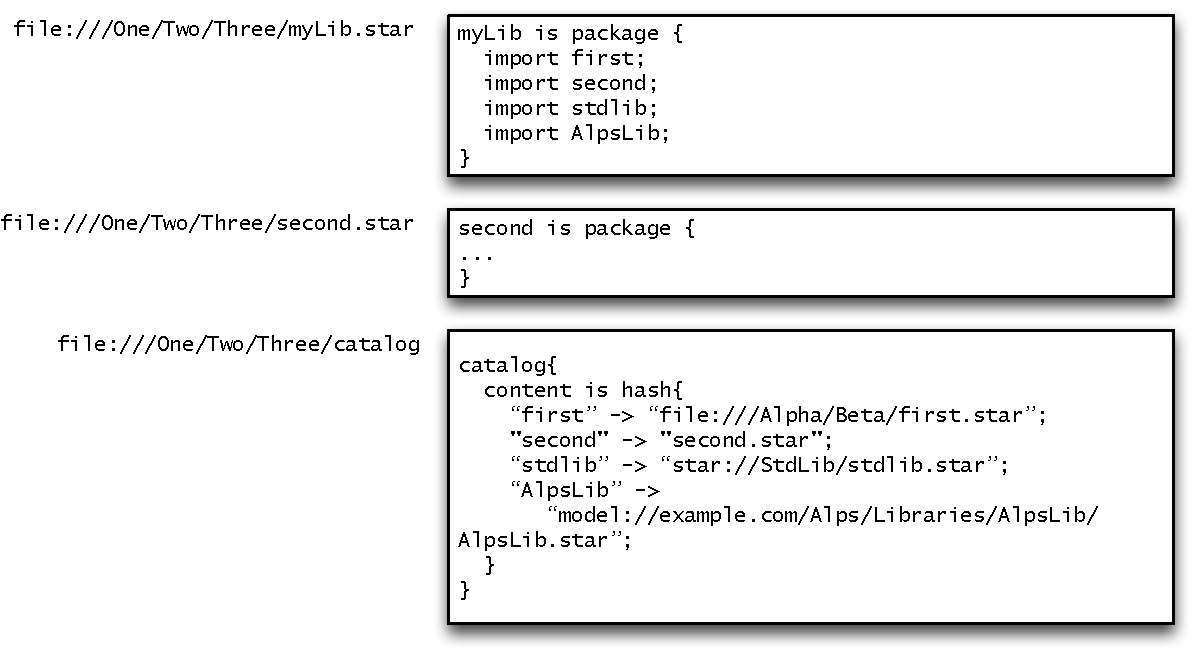
\includegraphics[width=\textwidth]{diagrams/library}
\caption{Library Structure}
\label{libraryFig}
\end{center}
\end{figure}

The library driver package typically has a standard form: it consists of a series of \ntRef{ImportStatement}s. The library is, in effect, defined by these \q{import}s.

The normal semantics of an \q{import} statement imply that the contents of all the \q{import}ed packages will be `re-exported' by the library driver package. The effect is that when the library driver package is imported, the entire contents of the library will be imported.

The second element of a library structure is the catalog. This typically contains the mapping from the names of packages to their URIs within the library `directory'.

Following the standard process of determining the catalog and URI of an \q{import}ed package, when the library driver \q{package} is imported, the library catalog will be accessed in order to interpret the contents of the library driver \q{package}.

\section{Resources and Catalogs}
\label{resources}

A package is an instance of a resource. A resource is any entity that can be identified. Examples of resources include package files (both source and compiled), and libraries. Resources need not be �static�: in principle, a service or a running application may also be viewed as a resource. However, in respect to the \Sr language, we are mostly concerned with \Sr package resources.

\subsection{Identifying Resources}
\index{Unified Resource Identifier}
The standard for identifying resources is the URI \cite{rfc2396}. \Sr uses URIs to locate source packages. Specifically, the \Sr language system \emph{must} support the URI schemes identified in Table~\vref{standardURISchemes}; however, it is free to support other schemes.

Program~\vref{uriProg} gives the \Sr definition of the standard \q{uri} type. This structure reflects the standard structure of a so-called hierarchic URI.  In addition to the `unpacked' \q{uri} structure, the \ntRef{TypeCoercion} expression:

\begin{lstlisting}
"..." as uri
\end{lstlisting}
represents a convenient way of writing URIs. The standard notation for URIs for supported schemes is supported by such expressions.

\begin{program}
\begin{lstlisting}
type uri is uri{
  scheme has type string;
  authority has type uriAuthority;
  path has type string;
  query has type string;
  fragment has type string
}

type uriAuthority is authority{
  user has type string;
  host has type string;
  port has type integer
} or noAuthority;
\end{lstlisting}
\caption{The Standard \q{uri} Type Description}\label{uriProg}
\end{program}

\begin{aside}
When a \q{uri} is used to denote an \q{import}ed package, the last part of the path must reflect the package name. I.e., if a package is called \q{pkg}, then the \q{uri} path must terminate in \q{.star}.
\end{aside}

\paragraph{Query Structure}
The \q{query} portion of a URI should take the form of a sequence of key=value pairs, separated by semi-colons. For example, a file URI with a VERSION attribute will look like:
\begin{lstlisting}
file:///foo/bar.star?VERSION=1.3;ACCESS=public
\end{lstlisting}

\subsubsection{Standard URI Schemes}
\label{standardSchemes}
The compiler recognizes a number of URI schemes as `standard': i.e., the compiler knows how to access the identified resources. In addition, the compiler also supports a technique for extending the set of known schemes with methods for locating the resources.
\begin{aside}
Technically, a URI contains no reliable indication of the physical location of the identified resource. However, for practical purposes it is often convenient to encode assumptions about physical location.
\end{aside}

The standard schemes supported by the compiler are listed in Table~\vref{standardURISchemes}.

\begin{table}[H]
\caption{Standard URI Schemes}\label{standardURISchemes}
\begin{center}
\begin{tabular}{|lll|}
\hline
Scheme&Type&Physical Location\\
\hline
\q{file:}&Local file&File path on system\\
\q{std:}&Built-in&Internal to compiler\\
\q{http:}&HTTP URL&Web page\\
\q{\$quoted\$:}&Quoted URI&Within URI's fragment\\
\q{star:}&Star source&File on local system\\
\hline
\end{tabular}
\end{center}
\end{table}

\begin{description}
\item[\q{file:}]A \q{file:} URI takes the form:
\begin{alltt}
file://\emph{Computer}/\emph{FilePath}
\end{alltt}
If the \emph{Computer} is omitted then the current machine that the compiler is executing on is assumed. If the \q{Computer} is not omitted, it may not be possible to access the remote computer.
\item[\q{std:}] A \q{std:} URI refers to resources that are properly part of the compiler itself. This are `hard-coded' in the sense that their location is established when the compiler is installed.
\item[\q{star:}] A \q{star:} URI refers to the default location that the compiler uses to find source files. This is often simply the working directory of the compiler; but may be configured with a command-line option.
\item[\q{http:}] A \q{http:} URI refers to a standard WEB URL. The compiler will attempt to access the resource by means of an HTTP request to the identified URL.
\item[\q{\$quoted\$:}] A \q{\$quoted\$} contains the source within the URI itself.

For example, the URI:
\begin{alltt}
$quoted$://hello#hello\%20is\%20package\%7b\%0a\%20\%20fun\%20hello
                                \%28\%29\%20is\%20\%22hello\%22\%3b\%0a\%7d
\end{alltt}
denotes the package:
\begin{lstlisting}
hello is package{
  fun hello() is "hello";
}
\end{lstlisting}
\begin{aside}
The standard notation for URIs requires that all the special characters used in a typical \Sr source must be encoded as \q{\%} hex pairs.

This URI is shown on two lines for convenience of display, but must actually be a contiguous sequence of characters.
\end{aside}
\begin{aside}
It is possible, if slightly redundant, to use quoted URIs to import a package:
\begin{lstlisting}
...
import "$quoted$://hello#hello%20is%20package
                 %7b%0a%20%20fun%20hello%28%29%20is%20%22
                 hello%22%3b%0a%7d";
...
\end{lstlisting}
However, a more important use of quoted URIs is to support dynamically compilation of \Sr in cases where the compiler is embedded.
\end{aside}
\end{description}

\subsubsection{Defining New Resource Schemes}
\label{newResoureScheme}
A new resource scheme may be introduced as a command line parameter using the \q{-DTRANSDUCER=} flag (see Section~\vref{compileFlags}).

The value of this flag is special form rule that takes the form:
\begin{alltt}
\emph{Ptn}==>\emph{Repl}
\end{alltt}
The syntax accepted by the pattern of the rule is the same as \ntRef{RegularExpression}; in particular, named groups are supported.

The purpose of this rule to map a new form of URI scheme into a predefined one.

In fact, the normal \q{star:} scheme can be expressed using a \q{TRANSDUCER} rule of the form:
\begin{alltt}
"star:(.*/)?([^/]+:V)==>file://\emph{tgtDir}/$V"
\end{alltt}
where \q{tgtDir} is the directory selected for finding source \Sr programs.

This particular rule locates the path component of the \q{star:} URI and translates it to a \q{file:}-based URI. It does not permit either a query or a fragment specifier; although these could be added they would have to be ignored.


\subsubsection{Resource Versions}
\label{uriVersion}
A resource URI may have a version indicator that identifies a particular version of the resource. The version indicator is a value associated with the \q{VERSION} keyword in the query portion of the URI.

For example, to specify version 2.1 of a resource, one might use the URI:
\begin{alltt}
file:///foo/bar.star?VERSION=2.1
\end{alltt}

The notation for version number is based on a release-version-update scheme.
\begin{figure}[htbp]
\begin{eqnarray*}
\ntDef{Version}&\arrow&\ntRef{Release}[\q{.}\ntRef{Version}[\q{.}\ntRef{Update}]]\\
\ntDef{Release}&\arrow&\ntRef{Digit}\sequence{}\ntRef{Digit}\\
\ntDef{Version}&\arrow&\ntRef{Digit}\sequence{}\ntRef{Digit}\\
\ntDef{Update}&\arrow&\ntRef{Digit}\sequence{}\ntRef{Digit}
\end{eqnarray*}
\caption{Version Numbering}
\label{versionNumberScheme}
\end{figure}
Version numbers are numeric, alphabetic version numbers are not permitted.

The requirement for any transducer that accesses a URI is either:
\begin{itemize}
\item if the URI references a specific version then that version of the resource should be accessed by the transducer;
\item if the URI does not reference a version, and if there are multiple versions of a resource, then the transducer must access the resource with the largest version number associated with it.
\end{itemize} 


\subsection{Packages and Paths}
\label{packagePath}
The URI used to identify a package must identify the package's name. Specifically, if the path component of a URI takes the form:
\begin{alltt}
Dir/Dir\sequence{/}Name.\emph{Ext}
\end{alltt}
then the name of the package -- as identified within the package source -- must be the same as the \q{Name} part of the package's URI.

This can be expressed more precisely as the substring of the URI's path gotten by removing both any leading folder names (separated by \q{/} characters) and any trailing extension (denoted as the remaining text following the last occurrence of a \q{.} character) must be the same as the name identified within the package source.

\subsection{Catalogs}
\label{catalog}
A catalog is a mapping from logical names to URIs. The \Sr language system uses this mapping to locate source files and compiled code when the corresponding resource is \q{import}ed by name. 

Catalogs offer an additional `level of indirection� between a name and the named entity. This indirection can be used, for example, to implement versioned access to resources. In addition, catalogs serve the role of �pulling together� the resources that a program or application needs into a coherent set.

Thus, when a package is imported by name, as in:
\begin{alltt}
world is package\{
  import hello;
  \ldots
\}
\end{alltt}
then the \Sr language system uses the catalog mapping to resolve the name \q{hello} to a \q{uri} in order to actually access the package. The \Sr type of \q{catalog} is shown in Program~\vref{catalogProg}.

\begin{program}
\begin{alltt}
type catalog is catalog\{
  content has type dictionary of (string,uri);
  version has type string;
  version default is nonString;
\}
\end{alltt}
\caption{The \q{catalog} Type}\label{catalogProg}
\end{program}

For example, the catalog definition:
\begin{alltt}
myCatalog is catalog\{
  content is dictionary of \{
    "hello" -> "file:///First/Second/hello.star";
    "stdlib" -> 
       "http://www.star-lang.org/extensions/StdLib/stdlib.star";
    "AlpsLib" -> 
       "model://example.com/Alps/Libraries/AlpsLib/AlpsLib.star";
    "star" -> "std:star.star"
  \}
\}
\end{alltt}
is a typical catalog denoting the programs available to a \Sr application. 

\subsubsection{Accessing Packages Using Catalogs}
\index{accessing packages with catalogs}
\index{catalog!accessing packages with}
The process of accessing a package involves:
\begin{enumerate}
\item If the package is identified by name, the URI of the package is looked up within the `current' catalog.
\begin{enumerate}
\item If the name is not present in the catalog, a fall-back catalog is searched if available.
\item If the name is not present, and there is no fall-back, exit with an error.
\end{enumerate}
\item The located URI is resolved against the URI of the current catalog. This allows catalogs themselves to contain relative URIs where possible.  This is the so-called target URI.

\item The target URI is dereferenced -- using a transducer -- and accessed. If the resource does not exist, or is not valid, exit with an error.
\item The catalog uri:
\begin{alltt}
"../catalog"
\end{alltt}
is resolved against the URI of the package containing the reference.
\begin{enumerate}
\item If a catalog exists in this location then that catalog is used to resolve references within the target resource.
\item If there is no catalog, then a catalog \emph{may} be synthesized by `exploring' the space around the target URI.
\end{enumerate}
\end{enumerate}

\subsubsection{Multiple Versions of a Package}
A code repository may contain multiple versions of a package. A programmer may specify a specific version to import by specifying the version in the package's URI: either directly in the \ntRef{ImportStatement} or in the catalog.

If no version is specified, then importing a package will always reference the package in the repository with the largest version number.

When compiling a package, the version of the package may be specified as a command-line option to the compiler or by defining a non-trivial value for the \q{version} attribute in the catalog structure.

However specified, the versions that a package is compiled against are fixed during the compilation of the package. I.e., when a package is compiled, it is compiled against specific versions of imported packages. When the package is later executed, the specific versions that were accessed at compile time are also used at run-time.

%!TEX root = reference.tex
\chapter{Conditions}
\label{conditions}
Conditions are used to express constraints. For example, a \q{where} pattern (see Section~\vref{guardPattern}) uses a condition to attach a semantic guard to a pattern. Conditions are also as guards on \emph{equations} (see Section~\vref{equations}) and in other forms of rule.


\begin{aside}
Conditions should not be confused with \q{boolean}-values expressions; the fundamental semantics of conditions is based on \emph{satisfiability} -- not \emph{evaluation} -- see Section~\vref{querySemantics}. However, a \q{boolean}-valued expression \emph{may} act as a degenerate example of a condition.
\end{aside}

Figure~\vref{conditionFormFig} illustrates the general forms of condition. 

\begin{figure}[htbp]
\begin{eqnarray*}
\ntDef{Condition}&\arrow&\ntRef{MatchesCondition}\\
%&\choice&\ntRef{MemberCondition}\\
&\choice&\ntRef{SearchCondition}\\
&\choice&\ntRef{IndexedSearch}\\
&\choice&\ntRef{ConjunctionCondition}\\
&\choice&\ntRef{DisjunctionCondition}\\
&\choice&\ntRef{ImpliesCondition}\\
&\choice&\ntRef{OtherwiseCondition}\\
&\choice&\ntRef{NegationCondition}\\
&\choice&\ntRef{ConditionalCondition}\\
&\choice&\ntRef{HasValueCondition}\\
&\choice&\ntRef{PresentCondition}\\
&\choice&\q{(}\ \ntRef{Condition}\ \q{)}\\
&\choice&\ntRef{Expression}
\end{eqnarray*}
\caption{Condition}
\label{conditionFormFig}
\end{figure}

\paragraph{Type Safety}
Unless it appears directly as an expression, the type of a condition is less interesting than whether the condition is \emph{type satisfiable}. In general, a condition is type satisfiable if it is consistent and it is potentially satisfiable. To further this we introduce the \satinf{} meta-predicate. A inference rule of the form:
\begin{prooftree}
\AxiomC{\rm{\emph{Condition}}}
\UnaryInfC{\typesat{E}{F}}
\end{prooftree}
declares that the form \emph{F} is valid in the context \emph{E} provided that \ntRef{Condition} is satisfied.

\section{Membership and Search}
\label{membershipCondition}


\subsection{Matches Condition}
The \q{matches} condition is a special condition that applies a pattern to a value. The condition is satisfied (see Section~\vref{querySemantics}) if the pattern matches the expression.

\begin{figure}[htbp]
\begin{eqnarray*}
\ntDef{MatchesCondition}&\arrow&\ntRef{Expression}\ \q{matches}\ \ntRef{Pattern}
\end{eqnarray*}
\caption{\q{matches} Condition}
\label{matchesPredicateFig}
\end{figure}

\subsubsection{Type Safety}
A \q{matches} condition is type safe if the types of the left hand side and right hand side are the same. Recall that the left hand side is an expression, whereas the right hand side is a pattern.

\begin{prooftree}
\AxiomC{\typeprd{E}{V}{T}}
\AxiomC{\typeprd{E}{P}{T}}
\BinaryInfC{\typesat{E}{V\ \q{matches}\ P}}
\end{prooftree}


\subsection{Has Value Condition}
\label{hasValueCond}
\index{has value operator@\q{has value} operator}
\index{accessing an optional value}
\index{option chaining}

The \q{has value} operator can be used as a \ntRef{Condition} to 'unwrap' an \q{option}al to access its contents in a safe way.

\begin{figure}[htbp]
\begin{eqnarray*}
\ntDef{HasValueCondition}&\arrow&\ntRef{Expression}\ \q{has value}\ \ntRef{Pattern}
\end{eqnarray*}
\caption{Option Has Value Condition}\label{optionUnwrapFig}
\end{figure}

The \q{has value} condition is satisfied if its right hand side expression is a \q{some} value and if its left hand pattern matches the contents of the optional value.

One common use of the \q{has value} condition is to 'bring into scope' a variable which represents the wrapped content of the \q{option}al value.

For example, suppose that \q{P} has the type given by
\begin{lstlisting}
P has type option of Person
\end{lstlisting}
then the condition in the equation:
\begin{lstlisting}
fun nameOf(P) where P has value PP is PP.name
\end{lstlisting}
unwraps the optional value of \q{P} into the non-optional \q{PP}. Note that this particular example can be better written:
\begin{lstlisting}
fun nameOf(P) is P?.name
\end{lstlisting}
since this makes the resulting type also \q{option}al.

\subsubsection{Type Safety}
A \q{has value} condition is type safe iff the expression on the left is consistent with the pattern on the right:
\begin{prooftree}
\AxiomC{\typeprd{E}{V}{\q{option of }T\sub{v}}}
\AxiomC{\typeprd{E}{P}{T\sub{v}}}
\BinaryInfC{\typesat{E}{V\ \q{has value}\ P}}
\end{prooftree}

\subsection{Present Condition}
\label{presentCond}
\index{present operator@\q{present} operator}
\index{accessing an optional value}
\index{option chaining}

The \q{present} operator can be used as a \ntRef{Condition} to test an \q{option}al to see if it has a value.

\begin{figure}[htbp]
\begin{eqnarray*}
\ntDef{PresentCondition}&\arrow&\q{present}\ \ntRef{Expression}
\end{eqnarray*}
\caption{Option Present Condition}\label{optionPresentFig}
\end{figure}

The \q{present} condition is satisfied if its right hand side expression is a \q{some} value.

One common use of the \q{present} condition is to test to see if an entry is present in a \q{dictionary}.

For example, suppose that \q{D} has value
\begin{lstlisting}
def D is dictionary of [1 -> "alpha", 2-> "beta"]
\end{lstlisting}
then the condition in the equation:
\begin{lstlisting}
fun isThere(K) is present D[K]
\end{lstlisting}
tests the the optional value of \q{D[K]} and is satisfied if the key \q{K} is present in the dictionary.

\subsubsection{Type Safety}
A \q{present} condition is type safe iff the expression on the left is an optional value:
\begin{prooftree}
\AxiomC{\typeprd{E}{V}{\q{option of }T\sub{v}}}
\UnaryInfC{\typesat{E}{\q{present}\ V}}
\end{prooftree}

\subsection{Search Condition}
\label{searchCondition}
A search condition is satisfied by finding elements of collections that meet some criterion.

\begin{figure}[htbp]
\begin{eqnarray*}
\ntDef{SearchCondition}&\arrow&\ntRef{Pattern}\ \q{in}\ \ntRef{Expression}
\end{eqnarray*}
\caption{Search Condition}
\label{searchFormFig}
\end{figure}

\begin{aside}
The collection being searched must implement the \q{iterable} contract -- see Section~\vref{iterableContract}.
\end{aside}

For example, the search condition:
\begin{lstlisting}
(X,"john") in parent
\end{lstlisting}
is satisfied (potentially multiple times) if there is a pair of the form:
\begin{lstlisting}[escapechar=|]
(|\emph{Val}|,"john")
\end{lstlisting}
`in' the collection identified as \q{parent}. If \q{parent} were defined as the list:
\begin{lstlisting}
list of [ ("alpha","john"), ("beta","peter"), ("gamma","john") ]
\end{lstlisting}
then the search condition has two solutions: one corresponding to \q{"alpha"} and the other to \q{"gamma"}.

\subsubsection{Type Safety}
A search condition is type safe if the type of the pattern corresponds to an element of the type of the collection. This is characterized by means of a  \ntRef{DependencyConstraint}.
\begin{prooftree}
\AxiomC{\typeprd{E}{P}{T\sub{e}}}
\AxiomC{\typeprd{E}{C}{\q{iterable over }T\ \q{determines}\ T\sub{e}}}
\BinaryInfC{\typesat{E}{P\ \q{in}\ C}}
\end{prooftree}
The type judgment of a \ntRef{SearchCondition} depends on the \q{iterable} contract (see Section~\vref{iterableContract}.

\subsection{Indexed Search Condition}
\label{indexedSearchCondition}
An \ntRef{IndexedSearch} condition is satisfied by finding elements of collections that match a pattern and where the index of the element within the collection is also matched against.

\begin{figure}[htbp]
\begin{eqnarray*}
\ntDef{IndexedSearch}&\arrow&\ntRef{Pattern}\,\q{->}\,\ntRef{Pattern}\ \q{in}\ \ntRef{Expression}
\end{eqnarray*}
\caption{Indexed Search Condition}
\label{indexedSearchFormFig}
\end{figure}

\begin{aside}
The collection being searched must implement the \q{indexed\_iterable} contract -- see Section~\vref{indexedIterableContract}.
\end{aside}

\ntRef{IndexedSearch} conditions allow the programmer to not only access the element of the collection but also its `position' within the collection. For example, the condition:
\begin{lstlisting}
(Ix->V where V>0 and Ix<10) in L
\end{lstlisting}
is satisfied for those elements in \q{L} which are greater than zero, and whose index is less than 10.

\begin{aside}
One of the important features of the \ntRef{IndexedSearch} is that the \ntRef{IndexSearch} could potentially be satisfied for each element of the collection -- depending, of course, on the patterns involved.
\end{aside}

\subsubsection{Type Safety}
An \ntRef{IndexedSearch} condition is type safe if the type of the pattern corresponds to an element of the type of the collection.
\begin{prooftree}
\def\ScoreOverhang{1pt}
\insertBetweenHyps{\hskip 1ex}
\AxiomC{\typeprd{E}{Ky}{T\sub{k}}}
\AxiomC{\typeprd{E}{Vl}{T\sub{v}}}
\AxiomC{\typeprd{E}{C}{\q{indexed\_iterable over }T\ \q{determines}\ (T\sub{k},T\sub{v})}}
\TrinaryInfC{\typesat{E}{Ky\,\q{->}\,Vl\ \q{in}\ C}}
\end{prooftree}
The type judgment of a \ntRef{IndexedSearch} condition depends on the \q{indexed\_iterable} contract (see Section~\vref{indexedIterableContract}).

\section{Logical Combinations}

\subsection{Conjunction Condition}
A conjunction -- using the \q{and} operator -- is satisfied iff both the left and right `arms' of the conjunction are satisfied.

\begin{figure}[htbp]
\begin{eqnarray*}
\ntDef{ConjunctionCondition}&\arrow&\ntRef{Condition}\ \q{and}\ \ntRef{Condition}\\
&\choice&\ntRef{Condition}\ \q{where}\ \ntRef{Condition}\\
\end{eqnarray*}
\caption{Conjunction Condition}
\label{conjunctionConditionFormFig}
\end{figure}

\begin{aside}
There is \emph{no} guarantee as to any order of evaluation of the arms of a condition. In particular, you may assume neither that the left is evaluated before the right, nor that both arms are, or are not, evaluated.
\end{aside}

\begin{aside}
The \q{where} variant of conjunction is syntactic convenience to allow conditions of the form:
\begin{lstlisting}
fun foo(rs) is (r in rs where r > 0) ? some(r) : none
\end{lstlisting}
which would otherwise be written:
\begin{lstlisting}
fun foo(rs) is (r in rs and r > 0) ? some(r) : none
\end{lstlisting}
or
\begin{lstlisting}
fun foo(rs) is ((r where r > 0) in rs) ? some(r) : none
\end{lstlisting}
\end{aside}

\subsubsection{Type Safety}
A conjunction is type safe iff the two arms of the conjunction are type safe.
\begin{prooftree}
\AxiomC{\typesat{E}{L}}
\AxiomC{\typesat{E}{R}}
\BinaryInfC{\typesat{E}{L\ \q{and}\ R}}
\end{prooftree}

\subsection{Disjunction Condition}
\label{disjunction}
\index{disjunctive condition}
\index{or condition@\q{or} condition}
A disjunction -- using the \q{or} operator -- is satisfied iff either the left or the right operands are satisfied.

\begin{figure}[htbp]
\begin{eqnarray*}
\ntDef{DisjunctionCondition}&\arrow&\ntRef{Condition}\ \q{or}\ \ntRef{Condition}
\end{eqnarray*}
\caption{Disjunction Condition}
\label{disjunctionConditionFormFig}
\end{figure}

\begin{aside}
There is no guarantee as to the order of evaluation of the left and right operands.
\end{aside}

\subsubsection{Type Safety}
A disjunction is type safe iff the two arms of the disjunction are type safe.
\begin{prooftree}
\AxiomC{\typesat{E}{L}}
\AxiomC{\typesat{E}{R}}
\BinaryInfC{\typesat{E}{L\ \q{or}\ R}}
\end{prooftree}

\subsection{Negated Condition}
A negation is satisfied iff the operand is \emph{not} satisfied.


\begin{figure}[htbp]
\begin{eqnarray*}
\ntDef{NegationCondition}&\arrow&\q{not}\ \ntRef{Condition}
\end{eqnarray*}
\caption{Negated Condition}
\label{negationConditionFormFig}
\end{figure}

\begin{aside}
If the negated query has any unbound variables in it then the meaning of the negated query is undefined.
\end{aside}

\subsubsection{Type Safety}
A negation is type safe iff the negated condition is type safe.
\begin{prooftree}
\AxiomC{\typesat{E}{N}}
\UnaryInfC{\typesat{E}{\q{not}\ N}}
\end{prooftree}

\subsection{Implies Condition}
An \emph{implication} condition -- using the \q{implies} operator -- is satisfied iff there is a solution to the right hand side for every solution to the left hand side.


\begin{figure}[htbp]
\begin{eqnarray*}
\ntDef{ImpliesCondition}&\arrow&\ntRef{Condition}\ \q{implies}\ \ntRef{Condition}
\end{eqnarray*}
\caption{Implies Condition}
\label{impliesConditionFormFig}
\end{figure}

For example, the state of having only sons can be defined as the condition that all ones children are male. This can be expressed using the condition:
\begin{lstlisting}
(P,X) in children implies X in male 
\end{lstlisting}

\begin{aside}
Like negation, an \q{implies} condition can never result in binding a variable to a value. It can only be used to verify a condition. Thus, to actually look for people who only have sons, a separate `generator' condition is needed. 

A query expression such as:
\begin{lstlisting}
(P,_) in children and (P,X) in children implies X in male
\end{lstlisting}
is effectively using the first `\q{(P,X) in children}' condition to find a person who has children, where the second implies condition verifies that \q{P }only has sons.
\end{aside}

\subsubsection{Type Safety}
A whenever condition is type safe iff the two arms are type safe.
\begin{prooftree}
\AxiomC{\typesat{E}{L}}
\AxiomC{\typesat{E}{R}}
\BinaryInfC{\typesat{E}{L\ \q{implies}\ R}}
\end{prooftree}


\subsection{Otherwise Condition}
\label{otherwiseQuery}
\index{query!otherwise@\q{otherwise}}

\begin{figure}[htbp]
\begin{eqnarray*}
\ntDef{OtherwiseCondition}&\arrow&\ntRef{Condition}\ \q{otherwise}\ \ntRef{Condition}
\end{eqnarray*}
\caption{Otherwise Condition}
\label{otherwiseConditionFormFig}
\end{figure}

An \q{otherwise} condition is semantically similar to a disjunction: an \q{otherwise} condition is satisfied if either the left hand side is satisfied or the right hand side is satisfied. However, it is actually extremely difficult to give a purely declarative semantics for the \q{otherwise} condition -- the right hand side of an \q{otherwise} \emph{must not be attempted} if there is at least one way of satisfying the left hand side.

For example, given a list \q{childOf}, the query:
\begin{lstlisting}
all Ch where (Ch,"john") in childOf otherwise noone matches Ch
\end{lstlisting}
results in an \q{array} containing all the children of \q{"john"}; unless \q{"john"} has no children, in which case the result will contain the singleton \q{noone}.\footnote{Assuming of course that \q{noone} is a type safe value for a \q{person}.}

More precisely, given a condition of the form:
\begin{lstlisting}[escapechar=|]
|\emph{Q\sub1}| otherwise |\emph{Q\sub2}|
\end{lstlisting}
if there exist \emph{any} instances that satisfy \q{\emph{Q\sub1}} condition then that is the \emph{only} way of satisfying the condition; otherwise the condition is satisfied if \q{\emph{Q\sub2}} can be satisfied.
\begin{aside}
The \q{otherwise} query can be used in situations similar to those where a \emph{left outer join} would be used. If \q{A} and \q{B} are two collections, then
\begin{lstlisting}
A otherwise B
\end{lstlisting}
(where \q{A} and \q{B} have suitable variables in common) is analogous to
\begin{lstlisting}
A left outer join B
\end{lstlisting}
assuming a suitable join condition.
\end{aside}

\subsubsection{Type Safety}
An \q{otherwise} condition is type safe iff the two arms of the condition are type safe.
\begin{prooftree}
\AxiomC{\typesat{E}{L}}
\AxiomC{\typesat{E}{R}}
\BinaryInfC{\typesat{E}{L\ \q{otherwise}\ R}}
\end{prooftree}

\subsection{Conditional Condition}
\label{conditionalQuery}
\index{conditional query constraint}
\index{dependent query}

A conditional condition is used when the actual condition to apply depends on a test. 

\begin{figure}[htbp]
\begin{eqnarray*}
\ntDef{ConditionalCondition}&\q{(}\ \ntRef{Condition}\ \q{?}\ \ntRef{Condition}\ \q{:}\ \ntRef{Condition}\q{)}
\end{eqnarray*}
\caption{Conditional Condition}
\label{conditionalConditionFig}
\end{figure}

For example, if the salary of an employee may be gotten from two different relations depending on whether the employee was a manager or not, the salary may be retrieved using a query:
\begin{lstlisting}
list of { all S where ( isManager(P) ? 
                  (P,S) in manager_salary :
                  (P,S) in employee_salary )
        }
\end{lstlisting}

As with conditional expressions (see Section~\vref{conditionalExpression}), the test part of the \ntRef{ConditionalCondition} is evaluated and, depending on whether the test is \emph{satisfiable} or not, the `then' branch or the `else' branch is used in the query constraint.

\begin{aside}
In the case that the `test' is satisfiable; then only solutions from the `then' branch will be considered for the overall query. Conversely, if the `test' is not satisfiable,\footnote{A normal \q{boolean}-valued expression is considered to be satisfiable iff it evaluates to \q{true}.} then only solutions from the `else' branch will be used for the overall query.
\end{aside}

\begin{aside}
\begin{aside}
The `test' part of a \ntRef{ConditionalCondition} is only satisfied once -- if there are multiple ways in which the `test' could be satisfied, only the first found is used.

The `test' may \emph{not} bind variables; if it does, those variables are in \emph{not} scope for the either the `then' branch or the `else' branch of the conditional.
\end{aside}
\end{aside}
\begin{aside}
\begin{aside}
However, if a variable is defined in \emph{both} arms of a \ntRef{ConditionalCondition} then the variable `escapes' the conditional itself. 

For example, the \ntRef{ConditionalCondition} above `defines' the variable \q{S} in both the `then' and `else' branch. Depending on the \q{isManager} test, the result of the query will either contain the value of a \q{manager\_salary} or an \q{employee\_salary}.
\end{aside}
\end{aside}

\begin{aside}
As with the \ntRef{OtherwiseCondition}, \ntRef{ConditionalCondition} can be useful in cases where defaults may apply.
\end{aside}

\subsubsection{Type Safety}
A \ntRef{ConditionalCondition} is type safe iff the three arms of the conditional are type safe.
\begin{prooftree}
\AxiomC{\typesat{E}{T}}
\AxiomC{\typesat{E}{L}}
\AxiomC{\typesat{E}{R}}
\TrinaryInfC{\typesat{E}{\q{(}\,T\ \q{?} L\ \q{:}\ R\,\q{)}}}
\end{prooftree}

\section{Satisfaction Semantics}
\label{querySemantics}
\index{query!semantics of}
\index{variable!in queries}

The semantics of conditions is based on \emph{satisfaction} -- for example, the answer to a query is based on the different ways that the condition part of the query may be satisfied. 

The satisfiability of a condition is not identical to the normal concept of evaluating \q{boolean}-valued expressions. In essence, a \ntRef{Condition} is satisfied if there is a binding for the unbound variables within the \ntRef{Condition} that `makes the \ntRef{Condition} true.

Variables that are bound as a result of satisfying a \ntRef{Condition} are often used to `produce' a value from the \ntRef{Condition}. For example, an \q{all} query has as value \emph{all} the tuples that satisfy the \ntRef{Condition} and the \q{anyof} query has as value any tuple that satisfies the \ntRef{Condition}.

\begin{aside}
Any variables that are defined within the query are assumed to be in scope across the entire query. This means that the types associated with variables' occurrences must all be consistent.

A variable may occur in an outer context as well as within the query. Such a variable is in scope within the query but is not defined by the query. As with repeated occurrences of variables, such `free variables' become constraints on the satisfaction of the query.
\end{aside}

\begin{description}
\item[A \ntRef{SearchCondition}] of the form:
\begin{lstlisting}[escapechar=|]
|\ntRef{Pattern}| in |\ntRef{Expression}|
\end{lstlisting}
is considered satisfiable for any value in the collection identified by \ntRef{Expression} that matches the \ntRef{Pattern}. 
\end{description}


The result of a query is expressed as the value of an expression. Each element of the result is obtained by evaluating the \emph{bound} expression in the context of the bindings of the variables arrived at during the satisfaction of the query constraint.

In the case of an \q{all} query and the \q{view} definition, the computed result contains the result of evaluating the bound expression for every possible way of satisfying the query.  The \q{one} query looks for just one way of solving the query constraint and a numerically bounded query looks for that many ways.\footnote{Of course, if the query asks for 10 results (say), there may not be that many answers.}

\begin{aside}
\index{conditions!relative order of terms}
\index{order of terms in conditions}
It is important to note that, in the case of a conjunction or disjunction, the relative order of terms is not relevant. For example the conditions
\begin{lstlisting}
X in male and ("fred",X) in parent
\end{lstlisting}
and
\begin{lstlisting}
("fred",X) in parent and X in male
\end{lstlisting}
have the same solutions -- are satisfied for the same bindings of the variable \q{X}.
\end{aside}

\subsubsection{Type Safety}
\label{querytypesatty}
A relational query is type if the type of the pattern is consistent with the type of the elements of the tuple.

\section{Standard Predicates}
\label{predicates}

The standard predicates are based on the \q{equality} and \q{comparable} contracts. These contracts define what it means for two values to be equal, or for one value to be lesser than another.

The \q{equality} contract is automatically implemented for any type that does not reference a program type (i.e., does not contain functions, procedures or other program values). However, the programmer may wish to explicitly implement \q{equality} for a user-defined type if equality for that type is not based on simple comparison of data structures. Such user-defined implementations override any defined by the language.

\subsection{The \q{equality} contract}
\label{equalityPredicates}
\index{equality predicates}
Equality is based on the \q{equality} contract -- see Program~\vref{equalityContract}. This defines the \q{boolean}-valued function: \q{=}. The complementary function \q{!=} is not defined as part of the \q{equality} contract; but is defined in terms of \q{=}.

\index{type!contracts!equality@\q{equality}}
\index{equality contract@\q{equality} contract}
\begin{program}
\begin{lstlisting}
contract equality over t is {
  (=) has type (t,t)=>boolean;
}
\end{lstlisting}
\caption{The Standard \q{equality} Contract\label{equalityContract}}
\end{program}

It is not necessary to explicitly implement the \q{equality} contract. The language processor automatically implements it for types that do not contain program values. However, it is possible to provide an explicit implementation for \q{equality} for cases where a more semantic definition of equality is desired.

\subsection{\q{=} -- equals}
\label{equalsPredicate}
\index{"=@\q{=} predicate}
\index{equality predicate}
\q{=} is part of the standard \q{equality} contract.
\begin{lstlisting}
(=) has type for all t such that (t,t) => boolean where equality over t
\end{lstlisting}
In general, equality is \emph{not} defined for all values. In particular, equality is not defined for functions, procedures and other program values.\footnote{Whether two expressions that denote functions of the same type denote the same function is, in general, not effectively decidable.}

\subsection{\q{!=} -- not equals}
\label{notEqualsPredicate}
\index{"!=@\q{"!=} predicate}
\index{inequality predicate}
\begin{lstlisting}
(!=) has type for all t such that (t,t) => boolean where equality over t
\end{lstlisting}
The \q{!=} predicate has a standard definition that makes it equivalent to a negated equality:
\begin{lstlisting}
X != Y is not X=Y
\end{lstlisting}

\subsection{The \q{comparable} contract}
\label{comparisonPredicates}

Comparison is based on the standard \q{comparable} contract -- see Program~\vref{comparableContract}.

Comparison is \emph{not} automatically implemented for all types -- the standard language provides implementations for the arithmetic types (\q{integer}s, \q{float}s etc.) and for the \q{string} type.


\index{type!contracts!comparable@\q{comparable}}
\index{comparable contract@\q{comparable} contract}
\begin{program}
\begin{lstlisting}
contract comparable over t is {
  (<) has type (t,t)=>boolean;
  (=<) has type (t,t)=>boolean;
  (>) has type (t,t)=>boolean;
  (>=) has type (t,t)=>boolean;
}
\end{lstlisting}
\caption{The Standard \q{comparable} Contract\label{comparableContract}}
\end{program}

\subsection{\q{<} -- less than}
\index{<@\q{<} predicate}
\begin{lstlisting}
(<) has type for all t such that (t,t)=>boolean where comparable over t
\end{lstlisting}

The \q{<} predicate is satisfied if the left argument is less than the right argument. The precise definition of less than depends on the actual implementation of the \q{comparable} contract for the type being compared; however, for arithmetic types, less than is defined as being arithmetic less than. For \q{string}s, one string is less than another if it is smaller in the standard lexicographic ordering of strings.

\subsection{\q{=<} -- less than or equal}
\index{=<@\q{=<} predicate}
\begin{lstlisting}
(=<) has type for all t such that (t,t)=>boolean where comparable over t
\end{lstlisting}

The \q{=<} predicate is satisfied if the left argument is less than or equals to the right argument.

\subsection{\q{>} -- greater than}
\index{>@\q{>} predicate}
\begin{lstlisting}
(>) has type for all t such that (t,t)=>boolean where comparable over t
\end{lstlisting}

The \q{>} predicate is satisfied if the left argument is greater than the right argument.

\subsection{\q{>=} -- greater then or equal}
\index{>=@\q{>=} predicate}
\begin{lstlisting}
(>=) has type for all t such that (t,t)=>boolean where comparable over t
\end{lstlisting}

The \q{>=} predicate is satisfied if the left argument is greater than or equal to the right argument.

%!TEX root = reference.tex
\chapter{Queries}
\label{queries}
\index{queries}
A \ntRef{Query} is an expression that denotes a value implicitly -- by operations and constraints on other identified values. Typically, the result of a query is an \q{list} but it may be of any \ntRef{Type} -- provided that it implements the \q{sequence} contract.

There are several `flavors' of query: the \q{all} query (shown in Figure~\vref{allSolutionsFig}) projects a subset over one or more base collections; the \emph{N} \q{of} query extracts a list containing at most \emph{N} tuples from a collection; and the \q{any} query extracts a tuple that satisfies the query.

The results of a query may be sorted and may be filtered for uniqueness.

\begin{figure}[htbp]
\begin{eqnarray*}
\emph{Expression}&\arrowplus&\ntRef{Query}\\
\ntDef{Query}&\arrow&\ntRef{SequenceQuery}\ \choice\ \ntRef{ReductionQuery}\ \choice\ \ntRef{SatisfactionQuery}
\end{eqnarray*}
\caption{Query Expression}\label{relationQueryFig}
\end{figure}

\section{Sequence Queries}
\label{sequenceQueries}

A \ntRef{SequenceQuery} returns a collection of answers -- either all of them or some subset of them.

\begin{figure}[htbp]
\begin{eqnarray*}
\ntDef{SequenceQuery}&\arrow&\ntRef{SequenceType}\ \q{of}\ \q{\{}\ntRef{QueryExpression}\ \q{\}}\\
\ntDef{QueryExpression}&\arrow&\ntRef{AllSolutionsQuery}\\
&\choice&\ntRef{BoundedCardinalityQuery}
\end{eqnarray*}
\caption{Sequence Query Expression}\label{sequenceQueryFig}
\end{figure}

\noindent
where the \ntRef{SequenceType} plays a similar role in identifying the type of the result to that in \ntRef{SequenceExpression}s. If the \ntRef{SequenceType} is the keyword \q{sequence} then the result type is determined by the context of the \ntRef{Query} expression. Otherwise, \ntRef{SequenceType} identifies the name of a \ntRef{Type} -- which must implement the \q{sequence} contract (see Program~\vref{sequenceContractDef}) -- that denotes the result type of the query.

There are two variants of the \ntRef{SequenceQuery} -- \ntRef{AllSolutionsQuery} which returns a collection of all the answers to a question and \ntRef{BoundedCardinalityQuery} which returns some bounded subset of the query answers.

\subsection{All Solutions Queries}
\label{allSolutions}
\index{query!all solutions}
The all solutions query expressions return results corresponding to all the different ways that a condition may be satisfied. There are variants corresponding to finding distinct solutions and having the result sets ordered.

\begin{figure}[htbp]
\begin{eqnarray*}
\ntDef{AllSolutionsQuery}&\arrow&[\,\q{all}\,|\,\q{unique}\,]\ \ntRef{Expression}\ \q{where}\ \ntRef{Condition}\ [\ntRef{Modifier}]\\
\ntDef{Modifier}&\arrow&\q{order}\ [\q{descending}]\ \q{by}\ \ntRef{Expression}\ [\q{using}\ \ntRef{Expression}]
\end{eqnarray*}
\caption{All Solutions Query}\label{allSolutionsFig}
\end{figure}

For example, given a \q{list} bound to the variable \q{Tble}:
\begin{lstlisting}
def Tble is list of [
  ("john",23),
  ("sam",19),
  ("peter",21)
]
\end{lstlisting}
the query
\begin{lstlisting}
list of { all Who where (Who,A) in Tble and A>20 }
\end{lstlisting}
is a \ntRef{SequenceQuery} over the \q{Tble} list defined above. Its value is the \q{list}:
\begin{lstlisting}
list of [
  "john",
  "peter"
]
\end{lstlisting}
\q{"john"} and \q{"peter"} are in the result because both \q{("john",23)} and \q{("peter",21)} are in \q{Tble} and satisfy the condition that \q{A} is greater than 20.

\index{queries!bound expression}
In principle, any expression may follow the \q{all} clause in a query. The `bound expression' may mention variables that are `bound' within the query constraint.

\subsubsection{Ordered Result Sets}
The \q{order by} modifier is associated with a \emph{path expression} -- like the bound expression it is evaluated in the context of a successful solution to the condition. The results of an \q{order}ed query expression are sorted according to the values of this path expression. The type of this expression must be one that admits to being compared -- i.e., the type must implement the \q{comparable} contract.

For example, to return an ordered \q{cons} list\footnote{The type of the resulting collection is depends on whether the \ntRef{Query} is governed by an enclosing \ntRef{SequenceType} if available, or of type \q{array} by default.} of people over the age of 20 we can use the query expression:
\begin{lstlisting}
cons of { all Who where (Who,A) in Tble and A>20
                        order by A}
\end{lstlisting}
which would give the result:
\begin{lstlisting}
cons of [
  "peter",
  "john"
]
\end{lstlisting}

The \q{using} modifier may be used in conjunction with the \q{order by} modifier to override the default concept of less than. If given, the \q{using} keyword should be followed by a \q{boolean}-valued function defined over the same type as the \q{order by} expression.

For example, to override the use of \q{<} in the \q{order by} query above, with say \q{>}, we can use:
\begin{lstlisting}
cons of { all Who where (Who,A) in Tble and A>20
                        order by A using (>)}
\end{lstlisting}
which would give the result
\begin{lstlisting}
cons of [
  "john",
  "peter"
]
\end{lstlisting}

\subsubsection{Duplicate Elimination}
\label{duplicateElim}
\index{eliminating duplicates in queries}
\index{query!eliminating duplicates}
\index{unique@\q{unique} queries}

The \q{unique} keyword is used, instead of the \q{all} keyword, to signal a query where duplicate elements are eliminated from the answer set.

For example, the query:
\begin{lstlisting}
list of { unique Sib where (P,Who) in parent and
                           (P,Sib) in parent and Who!=Sib }
\end{lstlisting}
would have the effect of eliminating duplication caused by the fact that most people have two recorded parents.

The \q{unique} query requires that the type of the `bound expression' implements the \q{comparable} contract -- i.e., that \q{<} is defined for the type.

\begin{aside}
The \q{unique} query is potentially more expensive than the \q{all} query -- since it involves post-processing the results as the \q{all} query to perform the duplicate elimination.
\end{aside}

%\subsubsection{Type Safety}
%By default, the type of an \q{all} query is an \q{array} type; it requires that the condition be type safe:
%\begin{prooftree}
%\AxiomC{\typeprd{E}{B}{T}}
%\AxiomC{\typesat{E}{C}}
%\BinaryInfC{\typeprd{E}{\q{all}\ B\ \q{where}\ C}{\q{list of }T}}
%\end{prooftree}
%
%The type safety rule for \q{unique} queries very similar, except that the bound element must be of a type that implements the \q{comparable} contract:
%\begin{prooftree}
%\AxiomC{\typeprd{E}{B}{T\ \q{where comparable over }T}}
%\AxiomC{\typesat{E}{C}}
%\BinaryInfC{\typeprd{E}{\q{unique}\ B\ \q{where}\ C}{\q{list of }T}}
%\end{prooftree}
%
%\index{query!sorted}
%\index{sorted queries}
%\index{creating a sorted list from a query}
%In the case of an \q{ordered} query, the path expression must implement \q{comparable} and the result is a \q{list}:
%\begin{prooftree}
%\AxiomC{\typeprd{E}{B}{T}}
%\AxiomC{\typesat{E}{C}}
%\AxiomC{\typeprd{E}{P}{P\sub{T}\ \q{where comparable over }P\sub{T}}}
%\TrinaryInfC{\typeprd{E}{\q{all}\ B\ \q{where}\ C\ \q{order by}\ P}{\q{list of }T}}
%\end{prooftree}
%
\subsection{Bounded Cardinality Queries}
The \emph{N} \q{of} quantifier delivers \emph{at most} N solutions to the query. For example, the query:
\begin{lstlisting}
list of { 5 of X where (P,X) in children }
\end{lstlisting}
returns an \q{list} of the first 5 children of \q{P}.

\begin{figure}[htbp]
\begin{eqnarray*}
\ntDef{BoundedCardinalityQuery}&\arrow&\ntRef{QueryQuantifier}\ \q{where}\ \ntRef{Condition}\ [\ntRef{Modifier}]\\
\ntDef{QueryQuantifier}&\arrow&[\,\q{unique}\,]\ \ntRef{Expression}\ \q{of}\ \ntRef{Expression}
\end{eqnarray*}
\caption{Bounded Cardinality Query}\label{boundedCardinalityFig}
\end{figure}

\subsubsection{Duplicate Elimination}
If the \q{unique} keyword is used with the bounded cardinality then duplication elimination is performed \emph{before} counting the results. I.e., a query of the form:
\begin{lstlisting}
list of { unique 5 of X where (P,X) in children }
\end{lstlisting}
is guaranteed to find 5 unique answers -- assuming that there are at least 5 unique ways of solving the \q{(P,X) in children} condition.

\subsubsection{Ordered Result Sets}
If the \q{ordered by} modifier is \emph{not} present, there is no defined ordering for the answers in the result. In particular, if \emph{N} answers are requested, they could be any \emph{N} answers that satisfy the condition.

If an \q{order by} clause is specified then the result consists of the `smallest' results. I.e., if there are 5 answers to the query:
\begin{lstlisting}
list of { all X where (P,X) in children }
\end{lstlisting}
then the query
\begin{lstlisting}
list of { 3 of X where (P,X) in children order by X }
\end{lstlisting}
results in an \q{array} of 3 elements that are guaranteed to be smaller or equal to any remaining answers.

If the \q{order descending} modifier is used then the `largest' results will be the ones returned.
\begin{aside}
Of course, in order to compute this smallest set, all the answers must first be computed. The result set sorted and only then the first elements picked.
\end{aside}

%\subsubsection{Type Safety}
%The type of a bounded query is a \q{list} type; it requires that the condition be type safe, and that the bound is an \q{integer}:
%\begin{prooftree}
%\AxiomC{\typeprd{E}{N}{\q{integer}}}
%\AxiomC{\typeprd{E}{B}{T}}
%\AxiomC{\typesat{E}{C}}
%\TrinaryInfC{\typeprd{E}{N\ \q{of}\ B\ \q{where}\ C}{\q{list of }T}}
%\end{prooftree}
%
%In the case of an \q{ordered} bounded query, the path expression must implement \q{comparable} and the result is a \q{list}:
%\begin{prooftree}
%\AxiomC{\typeprd{E}{N}{\q{integer}}\quad\typeprd{E}{B}{T}}
%\AxiomC{\typesat{E}{C}}
%\AxiomC{\typeprd{E}{P}{P\sub{T}\,\q{where comparable over }P\sub{T}}}
%\TrinaryInfC{\typeprd{E}{N\ \q{of}\ B\ \q{where}\ C\ \q{order by}\ P}{\q{list of }T}}
%\end{prooftree}

\section{Satisfaction Queries}
A \ntRef{Satisfaction} is used to find an individual that satisfies the condition. It returns a  \emph{single} result corresponding to a solution of the query -- as an \q{option}al value.

\begin{figure}[htbp]
\begin{eqnarray*}
\ntDef{SatisfactionQuery}&\arrow&\q{any of}\ \ntRef{Expression}\ \q{where}\ \ntRef{Condition}\ [\ntRef{Modifier}]
\end{eqnarray*}
\caption{Satisfaction Query}\label{satisfactionQueryFig}
\end{figure}

For example, to find a child of \q{P} one could use the expression:
\begin{lstlisting}
any of X where (P,X) in children
\end{lstlisting}

The \q{default} clause is used in the case that the \ntRef{Condition} is \emph{not} satisfiable. For example, assuming that we did not have a record of \q{"fred"}'s parents, then the query
\begin{lstlisting}
any of P where (P,"fred") in children default "not known"
\end{lstlisting}
would result in the answer \q{"not known"}.

\subsubsection{A Sorted Satisfaction Query}
The \q{order by} clause can be used to select the `smallest' solution to the query: the result of an \q{any of} query that is governed by an \q{order by} clause is effectively the \emph{least} solution to the query. If the \q{order descending} modifier is used then the result is the largest solution to the query.

For example, to find the youngest child of \q{"john"} we can use the query:
\begin{lstlisting}
any of X where ("john",X) in children and (X,A) in ages order by A
\end{lstlisting}

\subsubsection{Type Safety}
A satisfaction query's type is \q{option} of the type of the bound expression. As with other queries, it requires that the condition is safe:
\begin{prooftree}
\AxiomC{\typeprd{E$\,\cup{}\,$varsIn(C)}{B}{T}}
\AxiomC{\typesat{E}{C}}
\BinaryInfC{\typeprd{E}{\q{any of}\ B\ \q{where}\ C}{\q{option of }T}}
\end{prooftree}

In the case of an \q{order}ed satisfaction query, the path expression must implement \q{comparable}:
\begin{prooftree}
\AxiomC{\typeprd{E$\,\cup{}\,$varsIn(C)}{B}{T}}
\AxiomC{\typesat{E}{C}}
\AxiomC{\typeprd{E}{P}{P\sub{T}\ \q{where comparable over }P\sub{T}}}
\TrinaryInfC{\typeprd{E}{\q{any of}\ B\ \q{where}\ C\ \q{order by}\ P}{\q{option of }T}}
\end{prooftree}

\section{Reduction Query}
\label{reductionQuery}
\index{accumulating over a query}
\index{applying a function to the results of a query}

A \ntRef{ReductionQuery} differs from other forms of query in that the results of satisfying the \ntRef{Condition} are `fed' to a function rather than being returned as some form of collection.

\begin{figure}[htbp]
\begin{eqnarray*}
\ntDef{ReductionQuery}&\arrow&\q{reduction}\ \ntRef{Expression}\ \q{of}\ \ntRef{QueryExpression}
\end{eqnarray*}
\caption{Reduction Query}\label{reductionQueryFig}
\end{figure}

The reduction function should have the type:
\begin{lstlisting}
(t\sub{E},t\sub{E})=>t\sub{E}
\end{lstlisting}
were \q{t\sub{E}} is the type of the bound expression in the \ntRef{QueryExpression}.

For example, to add up all the salaries in a department, one could use a query of the form:
\begin{lstlisting}
reduction (+) of { all E.salary where E in employees }
\end{lstlisting}

\begin{aside}
The reducing function is only applied if there is more than one solution to the query. In this sense, it is closer in semantics to \q{leftFold1} than to \q{leftFold} -- see Section~\vref{foldableContract}.
\end{aside}

\begin{aside}
The \ntRef{ReductionQuery} may be used with all the normal variants of \ntRef{QueryExpression}.
\end{aside}
%!TEX root = reference.tex
\chapter{Numeric Expressions}
\label{numbers}
\index{expressions!arithmetic}

The basis of artithmetic expressions are several contracts: the \q{arithmetic} contract which provides definitions of the familiar `calculator' functions of \q{+}, \q{-}, \q{*} and \q{/}; the \q{math} contract which defines the extended set of mathematical functions; the \q{trig} contract which defines standard trigonometric functions; and the \q{bitstring} contract which gives definitions for bitwise manipulation of integer values.

\section{The \q{arithmetic} Contract}
\index{contract!arithmetic@\q{arithmetic} contract}
\label{arithmeticContract}

The \q{arithmetic} contract -- in Program~\vref{arithmeticContractProg} -- defines a minimum set of functions that should be supported by any arithmetic type.

\index{type!contracts! arithmetic@\q{arithmetic}}
\index{arithmetic contract@\q{arithmetic} contract}
\begin{program}
\begin{lstlisting}
contract arithmetic over t is {
  (+) has type (t,t)=>t;
  (-) has type (t,t)=>t;
  (*) has type (t,t)=>t;
  (/) has type (t,t)=>t;
  (%) has type (t,t) => t;
  abs has type (t)=>t;
  __uminus has type (t)=>t;
  zero has type t;
  one has type t;
}
\end{lstlisting}
\caption{The Standard \q{arithmetic} Contract\label{arithmeticContractProg}}
\end{program}

In addition to the \q{arithmetic} contract, the \q{math} contract -- defined in Program~\vref{mathContract} -- defines additional functions that go beyond the standard `calculator' functions.

\begin{aside}
In the standard system, the \q{arithmetic} contract is implemented for \q{integer}s, \q{long}s, \q{float}s and \q{decimal}s. However, it is possible for the programmer to implement \q{arithmetic} for other types.
\end{aside}

\subsection{\q{+} -- addition}
\label{plusFunction}
\index{arithmetic contract@\q{arithmetic} contract!+@\q{+}}
\q{+} is part of the standard \q{arithmetic} contract.
\begin{lstlisting}
(+) has type for all t such that (t,t)=>t where arithmetic over t
\end{lstlisting}

The \q{+} function adds its two arguments together and returns the result.

Depending on the type of the argument, different arithmetic will be invoked. For example
\begin{lstlisting}
X+4
\end{lstlisting}
denotes an \q{integer} addition (and \q{X} must be an \q{integer} variable); whereas
\begin{lstlisting}
Y+5.6
\end{lstlisting}
denotes a \q{float} addition.

\subsection{\q{-} -- subtraction}
\label{minusFunction}
\index{arithmetic contract@\q{arithmetic} contract!-@\q{-}}
\q{-} is part of the standard \q{arithmetic} contract.
\begin{lstlisting}
(-) has type for all t such that (t,t)=>t where arithmetic over t
\end{lstlisting}

The \q{-} function subtracts the second argument from the first and returns the result.

\subsection{\q{*} -- multiplication}
\label{timesFunction}
\index{arithmetic contract@\q{arithmetic} contract!*@\q{*}}
\q{*} is part of the standard \q{arithmetic} contract.
\begin{lstlisting}
(*) has type for all t such that (t,t)=>t where arithmetic over t
\end{lstlisting}
The \q{*} multiplies its two arguments together and returns the result.

\subsection{\q{/} -- division}
\label{divideFunction}
\index{arithmetic contract@\q{arithmetic} contract!/@\q{/}}
\q{/} is part of the standard \q{arithmetic} contract.
\begin{lstlisting}
(/) has type for all t such that (t,t)=>t where arithmetic over t
\end{lstlisting}
The \q{/} function divides the first argument by the second and returns the result.


\subsection{\q{abs} -- absolute value}
\label{abdFunction}
\index{arithmetic contract@\q{arithmetic} contract!abs@\q{abs}}
\q{abs} is part of the standard \q{arithmetic} contract.
\begin{lstlisting}
abs has type for all t such that (t)=>t where arithmetic over t
\end{lstlisting}

The \q{abs} function returns the absolute value of its argument.

\subsection{\q{\_\_uminus} -- unary minus}
\label{unaryMinus}
\index{arithmetic contract@\q{arithmetic} contract!uminus@\q{\_\_uminus}}
\q{\_\_uminus} is part of the standard \q{arithmetic} contract.
\begin{lstlisting}
(__uminus) has type for all t such that (t)=>t where arithmetic over t
\end{lstlisting}
The \q{\_\_uminus} function negates its argument. This function is rarely invoked explicitly by the programmer; it is automatically generated by the compiler with unary-minus expressions. I.e., the expression
\begin{lstlisting}
-X
\end{lstlisting}
is interpreted as a call to \q{\_\_uminus}:
\begin{lstlisting}
__uminus(X)
\end{lstlisting}

\subsection{\q{zero} -- arithmetic zero}
\label{zero}
\index{arithmetic contract@\q{arithmetic} contract!zero\q{zero}}
\q{zero} is part of the standard \q{arithmetic} contract.
\begin{lstlisting}
zero has type for all t such that t where arithmetic over t
\end{lstlisting}

The \q{zero} value returns the `additive zero' for the arithmetic type. It must obey the following axiom:

\begin{lstlisting}[escapechar=|]
|\emph{X}|+zero=|\emph{X}|
\end{lstlisting}
for all \q{\emph{X}} of type \q{t}.

The primary advantage of \q{zero} is that it makes it easier to write generic arithmetic functions; for example:

\begin{lstlisting}
fun fact(N) where N=zero is one
 |  fact(N) default is N*fact(N-one)
\end{lstlisting}


\subsection{\q{one} -- arithmetic unit}
\label{one}
\index{arithmetic contract@\q{arithmetic} contract!one\q{one}}
\q{one} is part of the standard \q{arithmetic} contract.
\begin{lstlisting}
one has type for all t such that t where arithmetic over t
\end{lstlisting}

The \q{one} value returns the `additive unit' for the arithmetic type.  It must obey the following axiom:

\begin{lstlisting}[escapechar=|]
|\emph{X}|*one=|\emph{X}|
\end{lstlisting}
for all \q{\emph{X}} of type \q{t}.

Like \q{zero}, the primary advantage of \q{one} is that it makes it easier to write generic arithmetic functions.

\section{The \q{largeSmall} Contract}
\label{largeSmall}
The \q{largeSmall} contract defines two values that are supposed to represent the largest and smallest legal values respectively of a type. The contract itself is very simple:
\begin{program}
\begin{lstlisting}
contract largeSmall over t is {
  largest has type t;
  smallest has type t;
}
\end{lstlisting}
\caption{The \q{largeSmall} Contract}\label{largeSmallProg}
\end{program}

The \q{largeSmall} contract is implemented for \q{integer}s, \q{long} integers, and \q{float} by default.

\subsection{\q{smallest} -- smallest value}
\begin{lstlisting}
smallest has type for all t such that t where largeSmall over t
\end{lstlisting}

The \q{smallest}  value is the smallest legal value of the type. For example, the smallest \q{long} value corresponds to $-2^{63}-1$.

\begin{aside}
It is not always possible to explicitly write down the smallest value of a type. In particular, it is not possible to write the smallest \q{long} value in decimal numbers.
\begin{aside}
It is possible, however, to write it in hexadecimal:
\begin{lstlisting}
0x8000000000L
\end{lstlisting}
\end{aside}
\end{aside}

\subsection{\q{largest} -- largest value}
\begin{lstlisting}
largest has type for all t such that t where largeSmall over t
\end{lstlisting}

The \q{largest}  value is the largest legal value of the type. For example, the largest \q{float} value is \q{1.7976931348623157E308}.

\begin{aside}
As with the \q{smallest} value; it is not necessarily the case that it is possible to explicitly write the \q{largest} value of a type.
\end{aside}

\section{Bit Manipulation Functions}
\label{bitString}

The \q{bitstring} contract defines a set of bit manipulation functions.

\begin{aside}
In the standard system, the \q{bitstring} functions are only implemented by the \q{integer} and \q{long} types.
\end{aside}

\begin{aside}
The bitstring functions require an explicit \q{import} before using them:
\begin{lstlisting}
import bitstring;
myPk is package { ...
\end{lstlisting}
\end{aside}

\index{type!contracts!bitstring@\q{bitstring}}
\index{bitstring contract@\q{bitstring} contract}
\begin{program}
\begin{lstlisting}
contract bitstring over t is {
    (.&.) has type (t,t)=>t;
    (.^.) has type (t,t)=>t;
    (.|.) has type (t,t)=>t;
    (.<<.) has type (t,t)=>t;
    (.>>.) has type (t,t)=>t;
    (.>>>.) has type (t,t)=>t;
    (.~.) has type (t)=>t;
    (.#.) has type (t)=>integer;
}
\end{lstlisting}
\caption{The Standard \q{bitstring} Contract\label{bitstringContractDef}}
\end{program}

\subsection{\q{.\&.} Bit-wise Conjunction}
\label{bitAnd}
\begin{lstlisting}
(.&.) has type for all t such that (t,t)=>t where bitstring over t
\end{lstlisting}

The \q{.\&.} operator returns the bit-wise conjunction of two values.

\subsection{\q{.|.} Bit-wise Disjunction}
\label{bitOr}
\begin{lstlisting}
(.|.) has type for all t such that (t,t)=>t where bitstring over t
\end{lstlisting}

The \q{.|.} operator returns the bit-wise disjunction of two values.

\subsection{\q{.\^{}.} Bit-wise Exclusive-or}
\label{bitXor}
\begin{lstlisting}
(.^.) has type for all t such that (t,t)=>t where bitstring over t
\end{lstlisting}

The \q{.\^{}.} operator returns the bit-wise exclusive of two values.

\subsection{\q{.<<.} Bit-wise Left Shift}
\label{bitLeft}
\begin{lstlisting}
(.<<.) has type for all t such that (t,t)=>t where bitstring over t
\end{lstlisting}

The \q{.<<.} operator left-shifts the left hand argument by the number of bits indicated in the right argument. It is effectively multiplication by a power of 2.

\subsection{\q{.>>.} Bit-wise Arithmetic Right Shift}
\label{bitRight}
\begin{lstlisting}
(.>>.) has type for all t such that (t,t)=>t where bitstring over t
\end{lstlisting}

The \q{.>>.} operator right-shifts the left hand argument by the number of bits indicated in the right argument. The most significant bit is replicated in the shift. It is effectively division by a power of 2.

\subsection{\q{.>>>.} Bit-wise Logical Right Shift}
\label{bitRightLogic}
\begin{lstlisting}
(.>>>.) has type for all t such that (t,t)=>t where bitstring over t
\end{lstlisting}

The \q{.>>>.} operator right-shifts the left hand argument by the number of bits indicated in the right argument. The most significant bits of the result are replaced by zero. This operator is sometimes known as logical right shift.

\subsection{\q{.\~\xspace.} Bit-wise Logical Complement}
\label{bitComplement}
\begin{lstlisting}
(.~.) has type for all t such that (t)=>t where bitstring over t
\end{lstlisting}

The \q{.\tlda.} operator forms the logical or 1's complement of its argument.

\subsection{\q{.\#.} Bit Count}
\label{bitCount}
\begin{lstlisting}
(.#.) has type for all t such that (t,t)=>t where bitstring over t
\end{lstlisting}

The \q{.\#.} operator computes the number of non-zero bits in its argument.


\section{Trigonometry Functions}
\label{trigContract}
The \q{trig} contract -- see Program~\vref{trigContractDef} -- defines standard trigonometry functions.

\begin{aside}
By default, the \q{trig} contract is only implemented over \q{float}ing point numbers.
\end{aside}

\begin{aside}
All the \q{trig} functions assume that the angles that they accept (or return) are expressed in radians.
\end{aside}

\index{type!contracts! trig@\q{trig}}
\index{trig contract@\q{trig} contract}
\begin{program}
\begin{lstlisting}
contract trig over t is {
  sin has type (t)=>t;
  asin has type (t)=>t;
  sinh has type (t)=>t;
  cos has type (t)=>t;
  acos has type (t)=>t;
  cosh has type (t)=>t;
  tan has type (t)=>t;
  atan has type (t)=>t;
  tanh has type (t)=>t;
}
\end{lstlisting}
\caption{The Standard \q{trig} Contract\label{trigContractDef}}
\end{program}

\subsection{\q{sin} -- Sine Function}
\begin{lstlisting}
sin has type for all t such that (t)=>t where trig over t
\end{lstlisting}

The \q{sin} function returns the Sine of its argument -- expressed in radians.

\subsection{\q{asin} -- Arc Sine Function}
\begin{lstlisting}
asin has type for all t such that (t)=>t where trig over t
\end{lstlisting}

The \q{asin} function returns the Arc Sine of its argument -- expressed in radians.

\subsection{\q{sinh} -- Hyperbolic Sine Function}
\begin{lstlisting}
sinh has type for all t such that (t)=>t where trig over t
\end{lstlisting}

The \q{sinh} function returns the hyperbolic sine of its argument -- expressed in radians.

The hyperbolic sine of X is defined to be $(e^X - e^{-X})/2$.

\subsection{\q{cos} -- Cosine Function}
\begin{lstlisting}
cos has type for all t such that (t)=>t where trig over t
\end{lstlisting}

The \q{cos} function returns the cosine of its argument -- expressed in radians.

\subsection{\q{acos} -- Arc Cosine Function}
\begin{lstlisting}
acos has type for all t such that (t)=>t where trig over t
\end{lstlisting}

The \q{acos} function returns the arc cosine of its argument -- expressed in radians.

\subsection{\q{cosh} -- Hyperbolic Cosine Function}
\begin{lstlisting}
cosh has type for all t such that (t)=>t where trig over t
\end{lstlisting}

The \q{cosh} function returns the hyperbolic cosine of its argument -- expressed in radians.

The hyperbolic cosine of X is defined to be $(e^X + e^{-X})/2$.

\subsection{\q{tan} -- Tangent Function}
\begin{lstlisting}
tan has type for all t such that (t)=>t where trig over t
\end{lstlisting}

The \q{tan} function returns the tangent of its argument -- expressed in radians.

\subsection{\q{atan} -- Arc Tangent Function}
\begin{lstlisting}
atan has type for all t such that (t)=>t where trig over t
\end{lstlisting}

The \q{atan} function returns the Arc Tangent of its argument -- expressed in radians.

\subsection{\q{tanh} -- Hyperbolic Tangent Function}
\begin{lstlisting}
tanh has type for all t such that (t)=>t where trig over t
\end{lstlisting}

The \q{tanh} function returns the hyperbolic tangent of its argument -- expressed in radians.

The hyperbolic tangent of X is defined to be $sinh(X)/cosh(X)$.

\section{Numeric Display Functions}
\label{numberDisplay}

The numeric display functions allow the representation of numbers as \q{string} values.

\subsection{\q{display} -- Display a number}
\label{displayNumFun}

The \q{display} function can be used to display a numeric value.
\begin{lstlisting}[escapechar=|]
display has type (|\ntRef{Type}|)=>string
\end{lstlisting}
The \q{display} function relies on the \q{ppDisp} function which is part of the \q{pPrint} contract -- see Program~\vref{ppContractProg}.

\subsection{\q{\_format} -- Format a number as a string}
\label{formatNumber}
\begin{lstlisting}[escapechar=|]
_format has type (|\ntRef{Type}|,string)=>pP
\end{lstlisting}
where \q{\emph{Type}} is one of \q{integer}, \q{long} or \q{float}.

The \q{\_format} function is part of the \q{formatting} contract -- see Program~\vref{formatContractProg}.

The format string for integral values determines how the number is formatted. For example, the result of
\begin{lstlisting}
"--$(-15):-   0;--"
\end{lstlisting}
is
\begin{lstlisting}
"--  -15--"
\end{lstlisting}

The grammar for legal formatting codes for integral values may be given in the regular expression:
\begin{lstlisting}
`[P+-]?([09 ,.])+[P+-]`
\end{lstlisting}
I.e., a sign specification, followed by digit specifications optionally mixed with thousands markers and periods, terminated by an optional sign specification.

The grammar for legal formatting codes for \q{float} values is a little more complex:
\begin{lstlisting}
`[P+-]?[09 ,.]+([eE][+-]?[09 ]+)?[P+-]?
\end{lstlisting}
I.e., the format string for \q{float} values permits the exponent to be printed as well as the mantissa. If the exponent part is missing and if the \q{float} value cannot be represented in the available precision without an exponent then an exception will be \q{raised}.

The complete list of formatting codes for formatting numeric values is:

\begin{description}
\item[\q{9}] A digit is displayed if it is significant. I.e., if it is non-zero or there is a non-zero digit to the left of the digit.
\item[\q{0}] A zero character is used for numeric values. It always results in a digit being displayed. For example, the value of
\begin{lstlisting}
"--$(5):00;--"
\end{lstlisting}
is the string
\begin{lstlisting}
"--05--"
\end{lstlisting}

\item[\q{\spce{}}] A space character is similar to the \q{0} code; except that a leading space is displayed instead of a leading zero. 

For example, the value of
\begin{lstlisting}
"--$(5):00;--"
\end{lstlisting}
is the string
\begin{lstlisting}
"-- 5--"
\end{lstlisting}

\begin{aside}
Signs are treated specially with the \q{\spce{}} code: any produced sign character is migrated past leading spaces -- with the result that the sign character is always abutted to the digits.

For example, the result of
\begin{lstlisting}
"--$(-15):-   0;--"
\end{lstlisting}
is
\begin{lstlisting}
"--  -15--"
\end{lstlisting}
The \q{\spce{}} code is especially useful for lining up columns of figures where a leading space is preferred over leading zeroes.
\end{aside}

\item[\q{.}] A period is displayed if there is a digit to the left.

This is used for showing currency values -- when they are represented internally as pennies but should be displayed as dollar values -- and for floating point numbers.
\item[\q{,}] A comma is displayed if there is a digit to the left. 

This is used for displaying values in the `thousands' notation. For example, the value of
\begin{lstlisting}
"--$(120345567):999,999,999,999;--"
\end{lstlisting}
is the string:
\begin{lstlisting}
"--120,345,567--"
\end{lstlisting}

\item[\q{-}] Is used to control how signed values are presented. If the value is negative then a \q{-} character is displayed; if the value is positive then a space is displayed.

\begin{aside}
The \q{-} \ntRef{FormatCode} may appear at either end of the display. A leading \q{-} results in the sign being displayed at the beginning -- before any digits -- and a trailing \q{-} results in the sign appended to the end.
\end{aside}

\begin{aside}
\begin{aside}
If no `sign' code is present in the \ntRef{FormattingSpec} then nothing is displayed if the value is positive or negative.
\end{aside}
\end{aside}

\item[\q{+}] Always results in a sign being displayed. If the value is negative then a \q{-} character is displayed; otherwise a \q{+} character is displayed.

Like the \q{-} code, the \q{+} may appear at either end of the display format.

\item[\q{P}] The \q{P} code uses parentheses on either end of the value to indicate a negative value. If the value is positive then spaces are appended to either end; otherwise the number is enclosed in \q{()}'s.

\begin{aside}
The \q{P} code should be placed at \emph{both} ends of the \ntRef{FormattingSpec}.
For example, the expression:
\begin{lstlisting}
"Balance: $Amnt:P999900.00P; remaining"
\end{lstlisting}
where \q{Amnt} had value -563 would result in
\begin{lstlisting}
"Balance: (05.63) remaining"
\end{lstlisting}
\end{aside}
\item[\q{X}] Causes the integer to be formatted as a hexadecimal number; and a hexadecimal digit is displayed if it is significant. I.e., if it is non-zero or there is a non-zero digit to the left of the digit.

For example, this can be used to display the Unicode equivalent of a character:
\begin{lstlisting}
"Unicode: $C/$(C as integer):XXXXX;"
\end{lstlisting}

\end{description}

\section{Additional Arithmetic Functions}
\label{mathContract}
The \q{math} contract -- see Program~\vref{mathContractDef} -- defines additional functions.

\begin{aside}
The \q{math} contract is not implemented by all number types; in particular, it is implemented by \q{integer}, \q{long} and \q{float}; but is not implemented by \q{decimal}.
\end{aside}

\index{type!contracts! math@\q{math}}
\index{math contract@\q{math} contract}
\begin{program}
\begin{lstlisting}
contract math over t is {
  min has type (t,t)=>t;
  max has type (t,t)=>t;
  random has type (t)=>t;
  sqrt has type (t)=>t;
  cbrt has type (t)=>t;
  ceil has type (t)=>t;
  floor has type (t)=>t;
  round has type (t)=>t;
  log has type (t)=>t;
  log10 has type (t)=>t;
  exp has type (t)=>t
  (**) has type (t,t) => t;
}
\end{lstlisting}
\caption{The Standard \q{math} Contract\label{mathContractDef}}
\end{program}

\subsection{\q{min} -- minimum value}
\begin{lstlisting}
min has type for all t such that (t,t)=>t where math over t
\end{lstlisting}

The \q{min} function returns the smaller of its two arguments.

\subsection{\q{max} -- maximum value}
\begin{lstlisting}
max has type for all t such that (t,t)=>t where math over t
\end{lstlisting}

The \q{max} function returns the larger of its two arguments.

\subsection{\q{sqrt} -- square root}
\begin{lstlisting}
sqrt has type for all t such that (t)=>t where math over t
\end{lstlisting}

The \q{sqrt} function returns the square root of its argument. If the argument is negative, the returned value is undefined.

\subsection{\q{cbrt} -- cube root}
\begin{lstlisting}
cbrt has type for all t such that (t)=>t where math over t
\end{lstlisting}

The \q{cbrt} function returns the cube root of its argument. Note that $-cbrt(X)=cbrt(-X)$.

\subsection{\q{ceil} -- ceiling}
\begin{lstlisting}
ceil has type for all t such that (t)=>t where math over t
\end{lstlisting}

The \q{ceil} function returns the nearest integral value that is equal to or larger than X.
\begin{aside}
For integral types,
\begin{lstlisting}
fun ceil(X)=X
\end{lstlisting}
\end{aside}

\subsection{\q{floor} -- floor}
\begin{lstlisting}
floor has type for all t such that (t)=>t where math over t
\end{lstlisting}

The \q{floor} function returns the nearest integral value that is equal to or smaller than X.
\begin{aside}
For integral types,
\begin{lstlisting}
fun floor(X)=X
\end{lstlisting}
\end{aside}

\subsection{\q{round} -- round to closest integral}
\begin{lstlisting}
round has type for all t such that (t)=>t where math over t
\end{lstlisting}

The \q{round} function returns the nearest integral value to its argument. 
\begin{aside}
For all values,
\begin{lstlisting}
fun round(X)=floor(X + 0.5)
\end{lstlisting}
\end{aside}


\subsection{\q{log} -- Natural Logarithm}
\begin{lstlisting}
log has type for all t such that (t)=>t where math over t
\end{lstlisting}

The \q{log} function returns the natural logarithm of its argument.

\subsection{\q{log10} -- Logarithm Base 10}
\begin{lstlisting}
log10 has type for all t such that (t)=>t where math over t
\end{lstlisting}

The \q{log10} function returns the base 10 logarithm of its argument.


\subsection{\q{exp} -- Natural Exponentiation}
\begin{lstlisting}
exp has type for all t such that (t)=>t where math over t
\end{lstlisting}

The \q{exp} function returns the value $e^X$.

\subsection{\q{random} -- random number generation}
\index{random number generation}
\begin{lstlisting}
random has type for all t such that (t)=>t where math over t
\end{lstlisting}

The \q{random} function returns a number in the half-open range [0,X) where X is the argument of the function.
\begin{aside}
The argument of the \q{random} function must be a positive number. However, it can be any `normal' kind of arithmetic value.
\end{aside}
The number generated is the next in a sequence of numbers that is typically \emph{pseudo-random}: i.e., not actually random but statistically indistinguishable from random.

The type of the returned result is the same as the type of its argument.

\subsection{\q{**} -- exponentiation}
\label{powerFunction}
\index{math contract@\q{math} contract!**@\q{**}}
\q{**} is part of the standard \q{math} contract.
\begin{lstlisting}
(**) has type for all t such that (t,t)=>t where math over t
\end{lstlisting}
The \q{**} function raises the first argument to the power of the second.

For example, the expression
\begin{lstlisting}
X**3
\end{lstlisting}
denotes the cube of \q{X}.

\section{Numeric Ranges}
\label{numericRange}
The \q{range} type defines a numeric range. It is useful primarily in loops; for example:
\begin{lstlisting}
X is list of {all Ix where Ix in range(0,10,1) }
\end{lstlisting}
has, as its value:
\begin{lstlisting}
list of [0, 1, 2, 3, 4, 5, 6, 7, 8, 9]
\end{lstlisting}

\begin{aside}
Ranges are half-open: they include their beginning value but do not include their terminator value. This permits simpler merging of ranges:
\begin{lstlisting}[escapechar=|]
range(0,10,1)++range(10,20,1) |\ensuremath{\equiv}| range(0,20,1)
\end{lstlisting}
\end{aside}

\subsection{The \q{range} Type}
The \q{range} type is defined in Program~\vref{rangeTypeProg}.
\begin{program}
\begin{lstlisting}
type range of t where arithmetic over t and comparable over t 
  is range(t,t,t);
\end{lstlisting}
\caption{The Standard \q{range} Type\label{rangeTypeProg}}
\end{program}

Note that this is a constrained type. It is a generic type but is only defined for type arguments that are \q{comparable} and which are defined over \q{arithmetic}.

The \q{range} type implements the \q{sizeable} contract (see Section~\vref{sizeableContract}), the \q{iterable} contract (see Section~\ref{iterableContract}) and the \q{concatenate} (see Section~\vref{concatenateContract}) contracts. This means that \q{range} is suitable for controlling for loops:
\begin{lstlisting}
for Ix in range(0,10,1) do
  logMsg(info,"$Ix")
\end{lstlisting}
as well as for using in queries such as above.

%!TEX root = reference.tex
\chapter{Strings}
\label{strings}
A string is a sequence of Unicode characters that denotes a fragment of text. This chapter focuses on the built-in functions that are based on the \q{string} type.

\section{The Structured String \q{pP} Type}
\label{ppType}
\index{pP type}
\index{type!pP@\q{pP}}
The \q{pP} type -- as defined in Program~\vref{ppTypeProg} -- denotes a `structured \q{string}' value where the structure may be used to represent lines, sub sequences and so on.
\begin{aside}
A primary purpose of the \q{pP} type is to permit simple formatting policies to be applied after the generation of the displayed form of a value.
\end{aside} 

\begin{program}
\begin{alltt}
type pP is 
     ppStr(string)
  or ppSequence(integer,cons of pP)
  or ppNl
  or ppSpace;
\end{alltt}
\caption{The Structured String \q{pP} type}\label{ppTypeProg}
\end{program}

The intended semantics of the constructors are:
\begin{description}
\item[\q{ppStr}] A literal string. Whenever a literal string is to be generated, the \q{ppStr} constructor is used to `hold' that string. For example, if the display of a value calls for an opening parenthesis, then the term:
\begin{alltt}
ppStr("(")
\end{alltt}
may be used to denote that.
\item[\q{ppSequence}]
The \q{ppSequence} constructor signals a subsequence in the display. It has two arguments: the first is an indentation amount, and the second is a \q{cons} list of sub-elements.

The indentation is used if a newline is generated within the subsequence. In that case, the new lines will be indented by the amount requested.
\item[\q{ppNl}]
Signal a new line in the displayed sequence. 
\begin{aside}
Simply signaling a new line does actually imply that a new line will be generated. New lines are generated depending on whether the client of the pretty print requires one in the actual displayed output.
\end{aside}
\item[\q{ppSpace}]
The \q{ppSpace} symbol denotes a `line-breakable' space. Multiple \q{ppSpace}s in sequence are equivalent to a single one.
\end{description}

\section{The \q{pPrint} contract}
\label{pPrintContract}
\index{pPrint contract@\q{pPrint} contract}
\index{pretty print contract}

The standard contract \q{pPrint}, shown in Program~\vref{ppContractProg} together with the \q{pP} type shown in Program~\vref{ppTypeProg}, is at the core of the standard method for displaying arbitrary values. 
\begin{program}
\begin{alltt}
contract pPrint over t is \{
  ppDisp has type (t)=>pP
\};
\end{alltt}
\caption{The Standard \q{pPrint} Contract}\label{ppContractProg}
\end{program}
The \Sr compiler will automatically generate implementations of the \q{pPrint} contract for all user-defined types. However, it will not override any implementations defined by the user.
\begin{aside}
It is not guaranteed that \emph{all} user-introduced types will be detected. In particular, some anonymous types are implicitly introduced by the programmer and these are not guaranteed to be detected.

However, if the compiler cannot find an implementation of \q{pPrint} then a default implementation will be used.
\end{aside}

The purpose of the \q{pPrint} contract is to support the standard \q{display} function -- see Section~\vref{displayFunction}. This, in turn, is used whenever a string \ntRef{Interpolation} expression is used.

\begin{aside}
One of the primary benefits of allowing programmers to define their own implementation of \q{pPrint} is to enable higher quality display of values. By defining \q{pPrint} for yourself, you can use application oriented display of your values.
\end{aside}


\subsection{Implementing the \q{pPrint} Contract}
As noted above, the \q{pPrint} contract is automatically implemented for standard types and for user-introduced types. However, it is quite possible to define one's own implementation. For example, supposing that values of the \q{tree} type:
\begin{alltt}
type tree of t is empty or node(tree of t,t,tree of t)
\end{alltt}
were intended to be display:
\begin{alltt}
\{ "alpha" "beta" "gamma" \}
\end{alltt}
instead of the default form:
\begin{alltt}
node(node(empty,"alpha",empty),"beta",node(empty,"gamma",empty))
\end{alltt}
then the following implementation of \q{pPrint} would ensure that such trees were displayed more conveniently:
\begin{alltt}
implementation pPrint over tree of \%t where pPrint over \%t is \{
  ppDisp(T) is ppSequence(2,cons of [ppStr("\{"), treeDisplay(T), ppStr("\}")])
\} using \{
  treeDisplay(empty) is ppSpace;
  treeDisplay(node(L,Lb,R)) is 
    ppSequence(0,cons of [treeDisplay(L), ppDisp(Lb), treeDisplay(R)]);
\}
\end{alltt}
\begin{aside}
Note how the use of \q{ppDisp} within the definition of \q{treeDisplay} will ensure that the display of tree labels may also be overridden with user-defined implementations of \q{pPrint}.
\end{aside}

\subsection{\q{display} -- display a value as a string}
\label{displayFunction}
\begin{alltt}
display has type (\%s)=>string
\end{alltt}
The \q{display} function returns a \q{string} representation of its value.

The \q{display} function is defined in terms of the \q{pPrint} contract defined in Program~\vref{ppContractProg}.
\begin{aside}
Although the system attempts to format the result in a way that can be parsed back; this is not guaranteed. In particular, this is not possible for any values that represent programs -- such as functions and procedures. Furthermore, user-defined implementations of \q{pPrint} may result in non-parseable output.
\end{aside}

\section{The \q{formatting} Contract}
\label{formatContract}
The \q{formatting} contract specifies the single \q{\_format} function which is intended to represent how values should be formatted.

The \q{formatting} contract itself is defined in Program~\vref{formatContractProg}. The result of a call to \q{\_format} is a structured \q{string}.

\begin{program}
\begin{alltt}
contract formatting over \%t is \{
  \_format has type (\%t,string)=>pP;
\}
\end{alltt}
\caption{The \q{formatting} Contract\label{formatContractProg}}
\end{program}



\begin{aside}
Normally, like \q{display}, calls to \q{\_format} are represented implicitly in string \ntRef{Interpolation} expressions.
\end{aside}
\subsection{Formatting Codes}
\label{formattingCodes}
A formatting code is a description of how a numeric or \q{string} valued expression should be displayed. Formatting codes allow more detailed control of the representation of the format in terms of minimum and maximum widths of output, the number of decimal places to show and the style of representing numbers -- including how negative numbers are displayed and the display of currencies.

A formatting code is introduced with a \q{:} character immediately after the \q{\$} form and is terminated by a \q{;} character. An invalid formatting code is ignored, and treated as though it were part of the quoted string proper.

Each type of value to be formatted may have different formatting codes; reflecting the natural variations in the type. For example formatting integral values may involve ways of managing the display of the sign of the number and formatting \q{date} values involves ways of show dates and times.

For example, to show a dollar value -- represented as pennies -- in \emph{accounting style} we can use:
\begin{alltt}
"Balance: \$Amnt:P999900.00P; remaining"
\end{alltt}
This format spec displays at least the four least significant digits of the variable \q{Amnt}. If the value of that variable is greater than 9999 then the leading digits are displayed also -- up to a maximum of eight digits. If the value of \q{Amnt} is negative then the number is displayed enclosed in parentheses.

For example, if \q{Amnt} had value -100000, then the value of the expression would be:
\begin{alltt}
Balance: (1000.00) remaining
\end{alltt}
If \q{Amnt} were 10000:
\begin{alltt}
Balance:  1000.00  remaining
\end{alltt}
\begin{aside}
Note the additional spaces: if the  \q{P} mode is used for representing sign, a white space character is generated for positive numbers. This facilitate straightforward alignment of columnar reports.
\end{aside}
If \q{Amnt} had value 45, then the result would be:
\begin{alltt}
Balance:  00.45  remaining
\end{alltt}
The \q{'0'} in the format will result in leading zeros being printed.
\begin{aside}
If a value cannot be represented in the delimited number of characters then the string:
\begin{alltt}
\q{*Error*}
\end{alltt}
is displayed; at least, as much of \q{*Error*} as is possible in the allocated space.\end{aside}


\subsection{\q{format} -- format a string for display}
\label{formatStringFunction}
\begin{alltt}
format has type (string,string)=>string
\end{alltt}

\begin{aside}
The \q{format} function for \q{string} values is normally invoked implicitly within a \q{string} \ntRef{Interpolation} expression. For example,
\begin{alltt}
"--\$Msg:C13;--"
\end{alltt}
is equivalent to the expression:
\begin{alltt}
"--"++format(Msg,"C13")++"--"
\end{alltt}
and has value:
\begin{alltt}
"--   freddie   --"
\end{alltt}
assuming that the value of the \q{Msg} variable is \q{"freddie"}.
\end{aside}

The format specification for \q{string} values is given in the regular expression:
\begin{alltt}
`[LCR][0-9]+`
\end{alltt}
where each control code is defined:
\begin{description}
\item[\q{L}] 
The value is shown left-aligned in the text.

The decimal value immediately after the \q{L} character is the size of the field.

If the displayed length of the number or string is less than that permitted; then the value is shown left-aligned. If the length of the value is greater than the size of the field then the text is truncated -- i.e., the first N characters of the value are used.

\item[\q{R}] The value is shown right-aligned in the text -- if the length of the value is less than the size of the field.

If the length of the value is greater than the size of the field then the text is truncated.

\item[\q{C}] The value is shown centered in the field. 
\end{description}

\begin{aside}
The \q{format} function is defined in terms of the \q{\_format} function and the \q{formatting} contract -- see Program~\vref{formatContractProg}.
\end{aside}

\section{Standard String Functions}
\label{simpleString}
In addition to certain specific string functions -- such as string concatenation -- the \q{string} type implements the \q{comparable} contract which enables \q{string} values to be compared. The \q{indexable} contract -- see Program~\vref{sizeableContract} -- is also implemented for \q{string}s, which means that the normal \q{[]} notation may be used to access the characters of a string.

\subsection{\q{isEmpty} -- test for empty string}
\label{stringEmptyFunction}
\q{isEmpty} is part of the standard \q{sizeable} contract (see Program~\vref{sizeableContract}):
\begin{alltt}
isEmpty has type (string)=>boolean
\end{alltt}
The \q{isEmpty} function returns true if its argument is the empty string. It's definition is equivalent to:
\begin{alltt}
isEmpty(X) is X="";
\end{alltt}

\subsection{\q{size} -- size of the string}
\label{stringSizeFunction}
\q{size} is part of the standard \q{sizeable} contract (see Program~\vref{sizeableContract}):
\begin{alltt}
size has type (string)=>integer
\end{alltt}
The \q{size} function returns the number of Unicode characters in the \q{string}. Note that this is not generally the same as the number of bytes in the string.

\subsection{\q{flattenPP} -- Flatten a Structured String}
\index{flattenPP@\q{flattenPP}}
\begin{alltt}
flattenPP has type (pP)=>string;
\end{alltt}
The \q{flattenPP} function takes a structured string and `flattens it' into a regular \q{string}.

\begin{aside}
This function is used by the standard functions \q{display} and \q{format} to convert the result of displaying or formatting a value into a \q{string}.
\end{aside}

\subsection{\q{<} -- less than}
\index{<@\q{<} predicate}
\begin{alltt}
(<) has type (string,string)=>boolean
\end{alltt}
\q{(<)} is part of the standard \q{comparable} contract -- see Program~\vref{comparableContract}.

String comparison is based on a lexicographic comparison: one \q{string} is less than another if its first character is less than the first character of the second -- irrespective of the actual lengths of the strings. Thus
\begin{alltt}
Abbbbbbb < B
\end{alltt}
because \q{A} is less than \q{B}. Characters are compared based on their \emph{code point} within the Unicode encoding.\footnote{This is the same concept of string ordering as that within Java\tm.}

\subsection{\q{<=} -- less than or equal}
\index{<=@\q{<=} predicate}
\begin{alltt}
(<=) has type (string,string)=>boolean
\end{alltt}
\q{(<=)} is part of the standard \q{comparable} contract -- see Program~\vref{comparableContract}.

The \q{<=} predicate for \q{string} values is satisfied if the left argument is less than or equals to the right argument under the lexicographic ordering.

\subsection{\q{>} -- greater than}
\index{>@\q{>} predicate}
\begin{alltt}
(>) has type (string,string)=>boolean
\end{alltt}
\q{(>)} is part of the standard \q{comparable} contract -- see Program~\vref{comparableContract}.
The \q{>} predicate is satisfied if the left argument is lexicographically greater than the right argument.

\subsection{\q{>=} -- greater then or equal}
\index{>=@\q{>=} predicate}
\begin{alltt}
(>=) has type (string,string)=>boolean
\end{alltt}
\q{(>=)} is part of the standard \q{comparable} contract -- see Program~\vref{comparableContract}.
The \q{>=} predicate is satisfied if the left argument is lexicographically greater than or equal to the right argument.

\subsection{\q{\_index} -- Index Character from String}
\label{indexString}
\q{\_index} is part of the standard \q{indexable} contract -- see Program~\vref{indexableContractDef}.
\begin{alltt}
_index has type (string,integer)=>char
\end{alltt}
The \q{\_index} function returns a character from a \q{string} value.

There is special syntax for indexing characters from a \q{string} -- as with indexing other kinds of \q{indexable} types -- one can use:
\begin{alltt}
S[ix]
\end{alltt}
instead of
\begin{alltt}
_index(S,ix)
\end{alltt}

\subsection{\q{\_slice} -- Substring}
\label{sliceString}
\q{\_slice} is part of the \q{sliceable} contract -- see Program~\vref{sliceableContractProg}.
\begin{alltt}
\_slice(string,integer,integer)=>string
\end{alltt}
The \q{\_slice} function extracts a substring from its first argument. The first character of the extracted substring is identified by the second argument; and the end point of the substring is identified by the third argument. An expression of the form:
\begin{alltt}
\_slice("this is a string",5,7)
\end{alltt}
returns the substring \q{"is"} -- corresponding to the two characters located at positions 5 and 6 in the source string.

There is a special notation for this functionality: the slice notation (see Section~\vref{sliceFunction}. For example, if the variable \q{S} is bound to the string \q{"this is a string"}, then the above expression may be written:
\begin{alltt}
S[5:7]
\end{alltt}

\subsection{\q{\_splice} -- Replace Substring}
\label{spliceString}
\q{\_splice} is part of the \q{sliceable} contract -- see Program~\vref{sliceableContractProg}.
\begin{alltt}
\_splice has type (string,integer,integer,string) => string
\end{alltt}
The \q{\_splice} function replaces a substring within its first argument. For example, the expression:
\begin{alltt}
\_splice("this is a string",5,7,"was")
\end{alltt}
has, as its value:
\begin{alltt}
"this was a string"
\end{alltt}

Like the \q{\_slice} notation, there is special syntax for this function -- when used as an action. The action:
\begin{alltt}
S[ix:tx] := U
\end{alltt}
is equivalent to the assignment:
\begin{alltt}
S := \_splice(S,ix,cx,U)
\end{alltt}

\subsection{\q{++} -- string concatenation}
\label{stringConcatFunction}
\q{++} is the standard string concatenation function. It is part of the \q{concatenate} contract (see Program~\vref{concatenateContractDef})
\begin{alltt}
(++) has type (string,string)=>string;
\end{alltt}

\index{string!interpolation}
Use of the \q{++} function over strings is implied by the \emph{string interpolation expression} (see Section~\vref{StringInterpolation}). For example, the string expression:
\begin{alltt}
"Count = \$count, Sum=\$sum"
\end{alltt}
is shorthand for
\begin{alltt}
"Count ="++display(count)++", Sum="++display(sum)
\end{alltt}

\subsection{\q{explode} -- Explode a string to chars}
\label{stringExplodeFunction}
The \q{explode} function is part of the \q{explosion} contract.
\begin{alltt}
explode has type (string)=>cons of char;
\end{alltt}
\begin{aside}
This version of the \q{explode} function is useful when performing complex operations over \q{string} values. For example, it can be more efficient to first of all \q{explode} a \q{string} before tokenizing the string.
\end{aside}

\subsection{\q{implode} -- Implode a cons list of chars to a string}
\label{stringImplodeFunction}
The \q{implode} function is part of the \q{explosion} contract.
\begin{alltt}
implode has type (cons of char)=>string;
\end{alltt}
The \q{implode} function takes a \q{cons} list of \q{char}s and constructs a \q{string} value from it.

\subsection{\q{reverse} -- Reverse the characters in a string}
\label{stringReverseFunction}
The \q{reverse} function is part of the \q{reversible} contract -- see Program~\vref{reversibleContractDef}.
\begin{alltt}
reverse has type (string)=>string
\end{alltt}

\subsection{\q{findstring} -- string search}
\label{findStringFunction}
\q{findstring} is used to determine the (next) location of a search token within a \q{string}.
\begin{alltt}
findstring has type (string,string,integer)=>integer;
\end{alltt}

\index{string!search within}
\index{finding substrings}
The \q{findstring} function searches a string for an occurrence of another string. The first argument is the string to search, the second is the search token, and the third is the integer offset where to start the search.

For example, the result of the expression:
\begin{alltt}
findstring("the lazy dog jumped over the quick brown fox","the",5)
\end{alltt}
is \q{25}.

If the search token is not present then \q{findstring} returns -1;

\subsection{\q{gensym} -- Generate Unique String}
\label{gensym}
\index{gensym standard function@\q{gensym} standard function}
\begin{alltt}
gensym has type (string)=>string
\end{alltt}
The \q{gensym} function is used to generate unique strings that have an arbitrarily high probability of being unique.

The generated string has a prefix consisting of the single argument, a middle which is a unique string generated based on a globally unique identifier identifying the current process and a counter.

The result is a string that has a high probability of being unique. It is guaranteed to be unique within the current processor.

\subsection{\q{spaces} -- Generate a string of spaces}
\label{spaces}
\index{spaces standard function@\q{spaces} standard function}
\begin{alltt}
spaces has type (integer)=>string
\end{alltt}

The \q{spaces} function generates a \q{string} containing only the space character -- \q{'\spce'}. For example, the value of
\begin{alltt}
spaces(3)
\end{alltt} 
is the \q{string}
\begin{alltt}
"   "
\end{alltt}

%!TEX root = reference.tex
\chapter{Sequences and Collections}
\label{lists}
\label{listExpressions}
\index{list expression}
\index{expressions!list}
There are many primary contracts that together relate to collections and sequences:
\begin{description}
\item[\q{concatenate}] defines what it means to concatenate two collections.
\item[\q{explosion}] defines the twin functions of explode and implode. Typically used to inspect and pack scalar entities.
\item[\q{foldable}] is a contract that defines the classic `fold' functions of leftFold, rightFold, leftFold1 and rightFold1.
\item[\q{indexable} and \q{sliceable}] are functions that define random access within a collection.
\item[\q{iterable} and \q{indexed\_iterable}] define processing a collection with a client function -- used for iterations and queries.
\item[\q{reversible}] defines the \q{reverse} function.
\item[\q{sequence}] is a core set of patterns and functions that defines what it means to process and/or build a collection sequentially.
\item[\q{sets}] define the set-oriented functions of intersection, union and complement.
\item[\q{sizeable}] is a pair of functions that define the size of a collection and whether the collection is empty or not.
\item[\q{sorting}] defines the sort function.
\item[\q{updateable}] is a set of functions that define the updating of collections by adding to a collection, merging collections, updating based on patterns and so on.
\end{description}
Many of these contracts are associated with special syntactic forms.
\begin{aside}
The term `collection' is used informally here. Not all types need implement all the contracts defined here. However, for a type to be considered a collection, it should implement all four contracts.
\end{aside}

In addition to the standard collection contracts, there are several standard types,  \q{list} and \q{cons} that represent basic forms of sequence.


\section{Sequence Notation}
\label{sequenceNotation}
The \q{sequence} contract has additional syntactic support in the form of specific sequence notation for expressions (see Section~\vref{sequenceExpression}) and patterns (see Section~\vref{sequencePattern}).

An expression of the form:
\begin{alltt}
[E\sub1\sequence{,}E\subn]
\end{alltt}
is equivalent to the expression:
\begin{alltt}
\_cons(E\sub1,\sequence{}\_cons(E\subn,\_nil())\sequence{})
\end{alltt}
Similarly, the pattern:
\begin{alltt}
[P\sub1\sequence{,}P\subn]
\end{alltt}is equivalent to the expanded pattern:
\begin{alltt}
\_pair(P\sub1,\sequence{}\_pair(P\subn,\_empty())\sequence{})
\end{alltt}
This notation makes literals involving the \q{sequence} contract easier to write.

\subsection{The \q{sequence} Contract}
\label{sequenceContract}
\index{sequence contract@\q{sequence} contract}
The \q{sequence} contract defines the equivalent of an abstract type that is `about' sequences. It is defined in Program~\vref{sequenceContractDef}. The elements of the \q{sequence} contract are sufficient to allow abstract sequential processing of sequences.

\begin{program}[hbtp]
\begin{alltt}
contract sequence over s determines e is \{
  \_empty has type ()<=s;
  \_pair has type (e,s)<=s;
  \_cons has type (e,s)=>s;
  \_apnd has type (s,e)=>s;
  \_back has type (s,e)<=s;
  \_nil has type ()=>s;
\}
\end{alltt}
\caption{The Standard \q{sequence} Contract}\label{sequenceContractDef}
\end{program}
\noindent
For example, the \q{reverse} function in Program~\vref{reverseProgram} is defined for any form of sequence; i.e., for any type that implements the \q{sequence} contract.
\begin{program}[hbtp]
\begin{alltt}
reverse has type for all e,t such that (t)=>t where
  sequence over t determines e
reverse(S) is let\{
  rev(\_empty(),R) is R;
  rev(\_pair(H,T),R) is rev(T,\_cons(H,R));
\} in rev(S,\_nil());
\end{alltt}
\caption{A \q{sequence} Reversal Function}\label{reverseProgram}
\end{program}
\begin{aside}
The \q{sequence} contract has a \emph{functional dependency} -- see Section~\vref{ContractFunctionalDependency}. This captures the intuition that sequences are about an element type; but the actual type of each element depends on the particular implementation of the \q{sequence}.
\end{aside}

\subsection{\q{\_empty} -- Empty Sequence Pattern}
\label{emptyPattern}
\index{sequence contract@\q{sequence} contract!empty@\q{empty}}
\begin{alltt}
\_empty has type for all e,t such that ()<=t 
                 where sequence over t determines e
\end{alltt}

The \q{\_empty} pattern is satisfied when matching an empty sequence.

\begin{aside}
The use of pattern abstractions is a normal feature of contracts that are aimed at defining an abstract type. 
\end{aside}

\subsection{\q{\_pair} -- Non-Empty Sequence Pattern}
\label{nonEmptyPattern}
\index{sequence contract@\q{sequence} contract!pair@\q{pair}}
\begin{alltt}
\_pair has type type for all e,t such that (e,t)<=t
                     where sequence over t determines e
\end{alltt}

The \q{\_pair} pattern is satisfied when matching an non-empty sequence. A successful match results in the head and tail part of the sequence also being match.

\subsection{\q{\_cons} -- Add to Front of Sequence}
\label{consFunction}
\index{sequence contract@\q{sequence} contract!cons@\q{cons}}
\begin{alltt}
\_cons has type type for all e,t such that (e,t)=>t
                     where sequence over t determines e
\end{alltt}
The \q{\_cons} function is used to `cons' an element to the front of a \q{sequence} -- returning a new sequence with the new element at the front.

\subsection{\q{\_apnd} -- Add to End of Sequence}
\label{appendFunction}
\index{sequence contract@\q{sequence} contract!apnd@\q{apnd}}
\begin{alltt}
\_apnd has type type for all e,t such that (t,e)=>t
                     where sequence over t determines e
\end{alltt}
The \q{\_apnd} function is used to append an element to the end of a \q{sequence}. I.e., a subsequent match against the \q{sequence} using the \q{\_pair} pattern will 'pick up' the newly appended element only after all existing elements have been removed.

\begin{aside}
Depending on the implementation type that backs a particular \q{sequence}, the performance of the \q{\_cons} and \q{\_apnd} functions may be radically different.
\end{aside}

\subsection{\q{\_back} -- Non-Empty Sequence Pattern}
\label{backPattern}
\index{sequence contract@\q{sequence} contract!back@\q{back}}
\begin{alltt}
\_back has type type for all e,t such that (t,e)<=t
                     where sequence over t determines e
\end{alltt}

Like the \q{\_pair} pattern, the \q{\_back} pattern is satisfied when matching an non-empty sequence. A successful match results in the last element of the sequence being matched -- as well as the front portion of the sequence.

\begin{aside}
Depending on the implementation type that backs a particular \q{sequence}, the performance of the \q{\_pair} and \q{\_back} patterns may be radically different.
\end{aside}

\subsection{\q{\_nil} -- Construct Empty Sequence}
\label{newFunction}
\index{sequence contract@\q{sequence} contract!cons@\q{cons}}
\begin{alltt}
\_nil has type type for all e,t such that ()=>t
                    where sequence over t determines e
\end{alltt}
The \q{\_nil} function is used to construct an empty instance of the sequence.

\section{Collection Notation}
Like the sequence notation, the collection notation is intended to allow collections that are not known to be sequences to be represented concisely in a type-independent way.

\section{The \q{concatenate} Contract}
\label{concatenateContract}
\index{concatenate contract@\q{concatenate} contract}
The \q{concatenate} contract defines a single function that implements the `concatenation' of two values together.

\begin{program}[H]
\begin{alltt}
contract concatenate over s is \{
  (++) has type (s,s)=>s;
\}
\end{alltt}
\caption{The Standard \q{concatenate} Contract}\label{concatenateContractDef}
\end{program}
\noindent

\subsection{\q{++} -- Concatenate Sequences}
\label{concatFunction}
\index{concatenate contract@\q{concatenate} contract!++@\q{++}}
\index{concatenate sequences}
\begin{alltt}
(++) has type for all s such that (s,s)=>s where sliceable over s
\end{alltt}
The meaning of \q{S++T} is a new sequence where the elements of \q{S} come `first' and the elements of \q{T} come `next'.

\section{The \q{reversible} Contract}
\label{reversibleContract}
\index{reversible contract@\q{reversible} contract}
The \q{reversible} contract defines a single function that implements the `reverse' of function.

\begin{program}[H]
\begin{alltt}
contract reversible over s is \{
  reverse has type (s)=>s;
\}
\end{alltt}
\caption{The Standard \q{reversible} Contract}\label{reversibleContractDef}
\end{program}
\noindent

\subsection{\q{reverse} -- Reverse Sequences}
\label{reverseFunction}
\index{reversible contract@\q{reversible} contract!reverse\q{reverse}}
\index{reverse sequences}
\begin{alltt}
\q{reverse} has type for all s such that (s)=>s where reversible over s
\end{alltt}
The meaning of \q{reverse(S)} is a new sequence where the elements of \q{S} are reversed.

\begin{aside}
The \q{reversible} contract is implemented for \q{list}s, \q{cons} lists and \q{string}s.
\end{aside}
\section{The \q{sets} Contract}
\label{setsContract}
The standard \q{sets} contract defines set operations over collections. 
\index{sets contract@\q{sets} contract}

\begin{program}[hbtp]
\begin{alltt}
contract sets over s is \{
  union has type (s,s)=>s;
  intersect has type (s,s)=>s;
  complement has type (s,s)=>s;
\}
\end{alltt}
\caption{The Standard \q{sets} Contract}\label{setContractDef}
\end{program}
\noindent

\subsection{\q{union} -- Union}
\label{unionFunction}
\index{sets contract@\q{sets} contract!union@\q{union}}
\index{union sequences}
\begin{alltt}
union has type for all s such that (s,s)=>s where sets over s
\end{alltt}
The meaning of \q{union(S,T)} is a new sequence consisting of elements of \q{S} merged with elements of \q{T}. Duplicate elements -- elements that appear in both \q{S} and \q{T} will not be duplicated in the result.

\begin{aside}
Although duplicates are eliminated as noted, if either of \q{S} or \q{T} already contains duplicates, then there may be duplicates in the result.
\end{aside}

\begin{aside}
There is no guarantee that the order of elements in the result reflects the order of elements in either of the sources of the \q{union} -- unless the type implementing the \q{sets} contract is already ordered.
\end{aside}

\subsection{\q{intersect} -- Intersection}
\label{intersectFunction}
\index{sets contract@\q{sets} contract!intersect@\q{intersect}}
\index{intersect sequences}
\begin{alltt}
intersect has type for all s such that (s,s)=>s where sets over s
\end{alltt}
The meaning of \q{intersect(S,T)} is a new sequence consisting of elements of \q{S} intersected with elements of \q{T}. Only elements that appear in both \q{S} and \q{T} will appear in the result.

\begin{aside}
There is no guarantee as to the order of elements in the result of \q{intersect}.
\end{aside}

\subsection{\q{complement} -- Complement}
\label{complementFunction}
\index{sets contract@\q{sets} contract!complement@\q{complement}}
\index{complement sequences}
\begin{alltt}
complement has type for all s such that (s,s)=>s where sets over s
\end{alltt}
The meaning of \q{complement(S,T)} is a new sequence consisting of elements of \q{S} which \emph{do not} occur within \q{T}.

\begin{aside}
There is no guarantee as to the order of elements in the result of \q{complement}.
\end{aside}


\section{The \q{sorting} Contract}
\label{sortingContract}
The \q{sorting} contract defines what it means to `sort' a collection. The contract itself is defined in Program~\vref{sortContractProg}.

\begin{program}[H]
\begin{alltt}
contract sorting over coll determines el is \{
  sort has type 
      (coll,(el,el)=>boolean) => coll;
\}
\end{alltt}
\caption{The \q{sorting} Contract\label{sortContractProg}}
\end{program}

\subsection{\q{sort} -- Sort a Collection}
\label{sortFunction}
\index{sorting contract@\q{sorting} contract!sort\q{sort}}
\index{sort a collection}
\begin{alltt}
sort has type for all el, coll such that
    (coll,(el,el)=>boolean) => coll where
       sorting over coll determines el
\end{alltt}

The \q{sort} function sorts a function -- using a supplied comparator function to compare elements. The comparator function should return true if the second argument is greater than or equal to the first.

\begin{aside}
The actual sort algorithm used is not represented here.
\end{aside}

The \q{sorting} contract is implemented for the \q{list} type and the \q{cons} list type.

\section{The \q{sizeable} Contract}
\label{sizeableContract}
The standard \q{sizeable} contract is defined for those collections that have a concept of size associated with them.

\index{type!contracts! sizeable@\q{sizeable}}
\index{sizeable contract@\q{sizeable} contract}

The \q{sizeable} contract -- which is defined in Program~\vref{sizeableContractProg} -- defines the functions \q{size} and \q{isEmpty}.

\begin{program}
\begin{alltt}
contract sizeable of t is \{
  size has type (t) => integer;
  isEmpty has type (t) => boolean;
\}
\end{alltt}
\caption{The Standard \q{sizeable} Contract\label{sizeableContractProg}}
\end{program}

\subsection{\q{size} -- Size of a \q{sizeable} Collection}
\label{sizeFunction}
\index{sizeable contract@\q{sizeable} contract!size@\q{size}}
\begin{alltt}
size has type for all t such that (t)=>integer where sizeable over t
\end{alltt}

The \q{size} function returns the number of elements of a \q{sizeable} collection. The precise meaning of the \q{size} function is likely to be type-specific; for example, for \q{string}s, the \q{size} of a \q{string} is the number of characters in the string.

\subsection{\q{isEmpty} -- Is a \q{sizeable} Collection Empty}
\label{isEmptyFunction}
\index{sizeable contract@\q{sizeable} contract!isEmpty@\q{isEmpty}}
\begin{alltt}
isEmpty has type for all t such that (t)=>boolean where sizeable over t
\end{alltt}
The \q{isEmpty} function returns \q{true} if the collection has no elements.

\section{The \q{indexable} Contract}
\label{indexableContract}
The \q{indexable} contract defines the functions that relate to the `indexable' expressions.

\begin{program}
\begin{alltt}
contract indexable over s determines (k,v) is \{
  _index has type (s,k)=>option of v;
  _set_indexed has type (s,k,v)=>s;
  _delete_indexed has type (s,k)=>s;
\end{alltt}
\caption{The Standard \q{indexable} Contract}\label{indexableContractDef}
\end{program}

The \q{indexable} contract defines what it means to access an element of a collection by index, and how such collections may be updated. The contract is parameterized both over the collection type and the index type -- a fact made use of to allow \q{dictionary} values to also be indexed.

\begin{aside}
Note that special notation supports high-level access to the \q{indexable} and \q{sliceable} contracts, as can be seen in Section~\vref{indexNotation} and Section~\vref{sequenceUpdate}.
\end{aside}

\subsection{\q{\_index} -- Index Element}
\label{indexFunction}
\index{indexable contract@\q{indexable} contract!_index@\q{\_index}}
\begin{alltt}
_index has type for all s,k,v such that (s,k)=>option of v
                where indexable over s determines (k,v)
\end{alltt}
\begin{aside}
The type of the index depends on the implementation of the contract. In the case of \q{list}s, the index is \q{integer}; and the first index is zero.
\end{aside}
\begin{aside}
If the index is not valid, for example if the index into a list is longer than the list, then \q{none} is returned.
\end{aside}

\subsection{\q{\_set\_indexed} -- Replace Element}
\label{indexReplaceFunction}
\index{indexable contract@\q{indexable} contract!_set_indexed@\q{\_set\_indexed}}
\index{replace element in collection}
\begin{alltt}
\_set\_indexed has type for all s,k,v such that (s,k,v)=>s
                        where indexable over s determines (k,v)
\end{alltt}
The \q{\_set\_indexed} function is used to represent the result of replacing an indexed element of a collection with a new value. The value returned is a new collection with every element identical to the original except that the ix\super{th} element is replaced.

If the index is out of range, i.e., if there is no element in the collection that corresponds to the requested index, then an error exception will be raised.

\subsection{\q{\_delete\_indexed} -- Remove Element}
\label{indexDeleteFunction}
\index{indexable contract@\q{indexable} contract!_delete_indexed@\q{\_delete\_indexed}}
\index{remove element from collection}

\begin{alltt}
\_delete\_indexed has type for all s,k,v such that (s,k)=>s
                           where indexable over s determines (k,v)
\end{alltt}
The \q{\_delete\_indexed} function is used to remove an element from a collection. The \q{\_delete\_indexed} function returns a collection with the identified element removed. The element to delete is identified by its key, not by the kay/value pair.

\begin{aside}
If the index is out of range, i.e., if there is no element in the collection that corresponds to the requested index, then an error exception may be raised -- depending on the implementation of the contract.
\end{aside}

\section{The \q{sliceable} Contract}
\label{sliceableContract}
The \q{sliceable} contract defines what it means to extract and update sub-sequences of collections. The contract -- defined in Program~\vref{sliceableContractProg} -- contains functions that extract a subsequence and replace a subsequence.
\begin{program}[htb]
\begin{alltt}
contract sliceable over t is \{
  \_slice has type (t,integer,integer)=>t;
  \_splice has type (t,integer,integer,t)=>t;
\}
\end{alltt}
\caption{The \q{sliceable} Contract\label{sliceableContractProg}}
\end{program}
As detailed below, the \q{sliceable} contract is supported by a `slice' notation that is based on the square bracket notation used to support indexing elements of collections.

\subsection{\q{\_slice} -- Extract Subsequence}
\label{sliceFunction}
\index{sliceable contract@\q{sliceable} contract!_slice@\q{\_slice}}
\index{extract subsequence of sequence}
\begin{alltt}
\_slice has type for all t such that (t,integer,integer)=>t
                 where sliceable over t
\end{alltt}
The meaning of \q{\_slice(S,Fr,To)} is that a subset of the sequence in \q{S} is extracted, starting with index position \q{Fr} up to -- but not including -- the index position \q{To}. The first index of the sequence is assumed to be zero.

If \q{To} is smaller than the length of the sequence then then the result will be shortened accordingly.

The \q{\_slice} function has a special syntax which is similar to that used for list indexing:
\begin{alltt}
C[Fr:To]
\end{alltt}
is equivalent to the expression
\begin{alltt}
\_slice(C,Fr,To)
\end{alltt}

\begin{aside}
The contract signature, and the type signature for \q{\_slice} do not mention the type of the elements of the sequence.
\end{aside}

\begin{aside}
For any sequence \q{S}, for any positive integers \q{F} $\ge0$ and \q{T}$\ge$\q{F}, the following identity is expected to hold for implementations of \q{\_slice}:
\begin{alltt}
S[F:T]++S[T:size(S)] = S
\end{alltt}
Note, in particular if \q{F} is greater than or equal to the \q{size} of the sequence then the result of \q{\_slice} will be an empty sequence. This is different to the behavior for \q{\_index} where an exception is \q{raise}d when the index is not present in the sequence.
\end{aside}

\begin{aside}
In addition to being implemented for \q{list}s, and \q{cons} lists, the \q{sliceable} contract is also implemented for \q{string}s. In the latter case, the \q{sliceable} contract defines the equivalent of sub-string and string-replace.
\end{aside}

\subsection{\q{\_splice} -- Replace Subsequence}
\label{spliceFunction}
\index{sliceable contract@\q{sliceable} contract!_splice@\q{\_splice}}
\index{replace subsequence of sequence}
\begin{alltt}
\_splice has type for all t such that (t,integer,integer,t)=>t
                  where sliceable over t
\end{alltt}
The meaning of \q{\_splice(S,Fr,To,R)} is that a subsequence of \q{S} is replace with \q{R}. Starting with index position \q{Fr}, the elements up until -- but not including -- the position \q{To} are replaced by \q{R}. The first index of the sequence is assumed to be zero.

If \q{To} is greater than or equal to the \q{size} of the sequence then the result will be to replace the remaining of the sequence with the new elements.

The \q{\_splice} function has a special syntax which is similar to that used for updating list elements:
\begin{alltt}
C[Fr:To] := S
\end{alltt}
is equivalent to the action
\begin{alltt}
C := \_splice(C,Fr,To,S)
\end{alltt}

\section{The \q{iterable} Contract}
\label{iterableContract}
The \q{iterable} contract defines what it means to `iterate' over a collection. The contract itself is defined in Program~\vref{iterateContractProg} and it makes use of the standard \q{IterState} type.

\begin{program}[H]
\begin{alltt}
contract iterable over coll determines el is \{
  \_iterate has type 
    for all r such that 
      (coll,(el,IterState of r)=>IterState of r,IterState of r) => 
        IterState of r;
\}

type IterState of t is NoneFound or NoMore(t) or ContinueWith(t);
\end{alltt}
\caption{The \q{iterable} Contract\label{iterateContractProg}}
\end{program}

The \q{iterable} contract defines a single function -- \q{\_iterate} -- which is used to `iterate' over a collection applying a client function to each element of the collection.

\subsection{\q{\_iterate} -- Iterate over collection}
\label{iterateFunction}
\index{iterable contract@\q{iterable} contract!\_iterate@\q{\_iterate}}
\index{iterate over collection}
\begin{alltt}
\_iterate has type 
    for all coll, el, r such that 
      (coll,(el,IterState of r)=>IterState of r,IterState of r) => 
        IterState of r 
      where iterable over coll determines el
\end{alltt}

The \q{\_iterate} function traverses a collection -- in an order that is `natural' to teh type of the collection -- applying a `client function' to each element.

The client function takes the form:
\begin{alltt}
fun(El,State) is NewState
\end{alltt}
where \q{El} is an element of the collection and \q{State} and \q{NewState} represent the `state' of the iteration and are of the type \q{IterState}.

\begin{aside}
The idea is that the client function `processes' the candidate in the context of previous invocations of the client function and returns a new state that reflects the result.
\end{aside}

\begin{description}
\item[\q{NoneFound}] The \q{NoneFound} enumerated symbol denotes an empty state. The client may return a \q{NoneFound} result if the state represents a null situation.

\begin{aside}
The \q{\_iterate} function should not interpret \q{NoneFound} as a signal to terminate the iteration.
\end{aside}
\item[\q{ContinueWith}]
The \q{ContinueWith} constructor is used to denote a partially completed state. The client function returns a \q{ContinueWith} when the denoted state may be augmented by further processing of elements of the collection.
\item[\q{NoMore}]
The \q{NoMore} constructor is used to denote a completed state. The client function returns a \q{NoMore} value when it intends to signal that no further processing of the collection by the \q{\_iterate} function should be performed.

The \q{\_iterate} function should terminate processing the collection if the client function returns an \q{NoMore} value.
\end{description}

For example, to find positive integer values in a collection this client function could be used:
\begin{alltt}
findPositive(X, ContinueWith(L)) where X>=0 is ContinueWith(cons(X,L));
findPositive(_,S) default is S;
\end{alltt}
\begin{aside}
The \q{\_iterate} function is used automatically for \ntRef{SearchCondition}s; however, the programmer is also free to explicitly use the \q{\_iterate} function.
\end{aside}
 
\begin{aside}
The precise form of the declaration of \q{\_iterate} within the \q{iterable} contract bears some additional explanation -- since it takes the form of an explicitly quantified type.

The \q{\_iterate} function is somewhat independent of the nature of the client function -- it applies the client function and terminates when the client function indicates that it is `done'. However, the precise state information that the client function is collecting is not relevant to the \q{\_iterate} function. In effect, the \q{\_iterate} function needs its client function to be generic.

In addition, since the semantics of the \q{\_iterate} function does not depend on the generic state that the client function collects it would not be correct to incorporate \q{r} as an additional type argument to the contract itself.

Hence the formulation of \q{\_iterate} as an explicitly universally quantified function \emph{within} the contract.
\end{aside}

\section{The \q{indexed\_iterable} Contract}
\label{indexedIterableContract}
The \q{indexed\_iterable} contract defines what it means to `iterate' over a sequence where elements have a location within the sequence. The contract itself is defined in Program~\vref{indexedIterateContractProg} and it also makes use of the standard \q{IterState} type seen in Program~\vref{iterateContractProg}.

\begin{program}[H]
\begin{alltt}
contract indexed\_iterable over s determines (k,v) is \{
  _ixiterate has type 
    for all r such that 
      (s,(k,v,IterState of r)=>IterState of r,IterState of r) => 
        IterState of r;
\}
\end{alltt}
\caption{The \q{indexed\_iterable} Contract\label{indexedIterateContractProg}}
\end{program}

The \q{indexed\_iterable} contract defines a single function -- \q{\_ixiterate} -- which is used to `iterate' over a sequence applying a client function to each element of the collection whilst keeping track of the index of the element within the collection that is being processed.

\subsection{\q{\_ixiterate} -- Iterate over collection}
\label{iterateFunction}
\index{indexed\_iterable contract@\q{indexed\_iterable} contract!\_ixiterate@\q{\_ixiterate}}
\index{iterate over collection}
\begin{alltt}
_ixiterate has type 
    for all coll,k,v,r such that 
      (coll,(k,v,IterState of r)=>IterState of r,IterState of r) => 
        IterState of r
      where indexed\_iterable over coll determines (k,v)
\end{alltt}

The \q{\_ixiterate} function traverses a collection -- in an order that is `natural' to the type of the collection -- applying a `client function' to each element. As it traverses the collection \q{\_ixiterate} keeps track of the index of the element within the collection.

The client function takes the form:
\begin{alltt}
fun(Ix,El,State) is NewState
\end{alltt}
where \q{Ix} is a value that denotes the `position' of the element within the collection, \q{El} is an element of the collection and \q{State} and \q{NewState} represent the `state' of the iteration and are of the type \q{IterState}.

The interpretation of the \q{State} is the same as for the \q{iterable} contract.

For example, to find the location within a \q{cons} list of an element that is greater than zero we can use the client function:
\begin{alltt}
indexOfPositive(Ix,X, ContinueWith(L)) where X>=0 is ContinueWith(cons(Ix,L));
indexOfPositive(_,_,S) default is S;
\end{alltt}
\begin{aside}
The \q{\_ixiterate} function is used automatically in \ntRef{IndexedSearch} conditions; however, the programmer is also free to explicitly use the \q{indexed\_iterable} contract.
\end{aside}

\section{The \q{mappable} Contract}
\label{mappableContract}
The \q{mappable} contract defines what it means to be able to apply a function over a collection. It contains a single \q{map} function:

\begin{program}[H]
\begin{alltt}
contract mappable over c is \{
  map has type for all e,f such that ((e)=>f,c of e) => c of f;
\}
\end{alltt}
\caption{The \q{mappable} Contract\label{mapContractProg}}
\end{program}

\subsection{\q{map} -- Apply a transformation to a collection}
\label{mapFunction}

The \q{map} function applies a function to a collection to produce a new collection. Its type is given by:
\begin{alltt}
map has type for all e,f such that ((e)=>f,c of e) => c of f where
  mappable over c
\end{alltt}
For example, we can use \q{map} to construct a list of \q{string} representations of \q{integer} values by mapping \q{display} (see \vref{displayFunction}):

\begin{alltt}
map(list of [1,2,3,4],display)
\end{alltt}
the value of which is the \q{list}:
\begin{alltt}
list of ["1","2","3","4"]
\end{alltt}

Note the slightly unusual quantification over the collection type. The \q{map} function must be able to accept a generic function as its transformation function.

\section{The \q{filterable} Contract}
\label{filterableContract}
The \q{filterable} contract contains a single function -- \q{filter} -- that can be used to filter elements from a collection.


\begin{program}[H]
\begin{alltt}
contract filterable over t determines e is \{
  filter has type ((e)=>boolean,t) => t
\}
\end{alltt}
\caption{The \q{filterable} Contract\label{filterContractProg}}
\end{program}


\subsection{\q{filter} -- Apply a predicate to a collection}
\label{filterFunction}

The \q{filter} function applies a predicate to a collection to produce a new collection -- containing only elements that satisfy the predicate. Its type is given by:
\begin{alltt}
filter has type for all e,t such that ((e)=>boolean,t) => t where
  filterable over t determines e
\end{alltt}
For example, we can use \q{filter} to eliminate odd numbers from a list of \q{integer}s:
\begin{alltt}
filter(list of [1,2,3,4,5,6],fn X=>X\%2=0)
\end{alltt}
which has value:
\begin{alltt}
list of [2,4,6]
\end{alltt}

\section{The \q{foldable} Contract}
\label{foldableContract}
The \q{foldable} contract defines another variant of iterating over collections while aggregating. The \q{foldable} contract defines two functions: \q{leftFold} and \q{rightFold}.

\begin{program}[H]
\begin{alltt}
contract foldable over c determines e is \{
  leftFold has type for all st such that ((st,e)=>st,st,c)=>st;
  leftFold1 has type ((e,e)=>e,c) => e;
  rightFold has type for all st such that ((e,st)=>st,st,c)=>st;
  rightFold1 has type ((e,e)=>e,c)=>e;
\}
\end{alltt}
\caption{The \q{foldable} Contract\label{foldableContractProg}}
\end{program}

For example, to add together a collection of \q{integer}s, one can use a \q{leftFold} (or equivalently a \q{rightFold}) expression:
\begin{alltt}
leftFold((+),0,list of [1, 2, 3, 4])
\end{alltt}
which has value \q{10}.

\begin{aside}
The appropriateness of using \q{leftFold} or \q{rightFold} depends on whether the function being applied is left associative or right associative. If the function is left associative, it is normally better (in the sense of being closer to what one might expect) to use \q{leftFold}.

The \q{leftFold1} and \q{rightFold1} variants are used in cases where there is no natural `zero' for the function being applied.

Some functions are commutative -- like \q{(+)} -- in which case the value returned by \q{leftFold} is equal to the value returned by \q{rightFold}.
\end{aside}

\subsection{\q{leftFold} -- Aggregate from the Left}
\label{leftFold}
The \q{leftFold} function reduces a sequence by successively applying a function from the beginning of the sequence.
\begin{alltt}
leftFold has type for all e,c,s such that
    ((s,e)=>s,s,c) => s where foldable over c determines e
\end{alltt}
The client function takes the form:
\begin{alltt}
leftClient(\emph{Acc},\emph{El}) is \emph{Acc'}
\end{alltt}
where \q{\emph{Acc}} is the accumulated result so far, \q{\emph{El}} is successive elements of the collection and \q{\emph{Acc'}} is the result of applying the client function to the element.

\subsection{\q{leftFold1} -- Non-zero Aggregate from the Left}
\label{leftFold1}
The \q{leftFold1} function reduces a sequence by successively applying a function from the beginning of the sequence. The first element of the sequence is used as the initial `state':
\begin{alltt}
leftFold1 has type for all e,c such that
    ((e,e)=>e,c) => c where foldable over c determines e
\end{alltt}
The client function takes the form:
\begin{alltt}
leftClient(\emph{Acc},\emph{El}) is \emph{Acc'}
\end{alltt}
where \q{\emph{Acc}} is the accumulated result so far, \q{\emph{El}} is successive elements of the collection and \q{\emph{Acc'}} is the result of applying the client function to the element.

\begin{aside}
The client function has a simpler form of type than that for \q{leftFold}. In particular, the types of both arguments and the result are identical. This is because \q{leftFold1} uses the first element of the sequence as the initial seed of the computation -- as opposed to an externally provided zero.
\end{aside}

\begin{aside}
If the sequence is empty then \q{leftFold1} will raise an exception.
\end{aside}

\begin{aside}
The standard contract for \q{foldable} includes a \emph{default} implementation of \q{leftFold1}. This default implementation is used in cases where a concrete implementation does not include a definition for \q{leftFold1}.
\end{aside}

\subsection{\q{rightFold} -- Aggregate from the Right}
\label{rightFold}
The \q{rightFold} function reduces a sequence by successively applying a function from the end of the sequence.
\begin{alltt}
rightFold has type for all e,c,s such that
    ((e,s)=>s,s,c) => s where foldable over c determines e
\end{alltt}
The client function takes the form:
\begin{alltt}
rightClient(\emph{El},\emph{Acc}) is \emph{Acc'}
\end{alltt}
where \q{\emph{Acc}} is the accumulated result so far, \q{\emph{El}} is succesive elements of the collection and \q{\emph{Acc'}} is the result of applying the client function to the element.

\begin{aside}
Note that the order of the arguments in the left client and the right client is different: the right client function has the `element' argument first whereas the left client has the element argument second.

This reflects the difference in expected associativity of the clients.
\end{aside}

\subsection{\q{rightFold1} -- Non-zero Aggregate from the Right}
\label{rightFold1}
The \q{rightFold1} function reduces a sequence by successively applying a function from the end of the sequence. The last element of the sequence is used as the initial `state':
\begin{alltt}
rightFold1 has type for all e,c such that
    ((e,e)=>e,c) => c where foldable over c determines e
\end{alltt}

\begin{aside}
The client function has the same form as that for \q{leftFold1}; in particular its type is the same. However, the order of arguments is different: in particular, the client function should take the form:
\begin{alltt}
rightClient(\emph{El},\emph{Acc}) is \emph{Acc'}
\end{alltt}
with successive elements being passed in to the first argument and the accumulated state in the second.
\end{aside}

\begin{aside}
If the sequence is empty then \q{rightFold1} will raise an exception.
\end{aside}

\begin{aside}
The standard contract for \q{foldable} includes a \emph{default} implementation of \q{rightFold1} -- which is based on the non-default implementation of \q{rightFold}.
\end{aside}

%\section{The \q{iotaC} Sequence Generation Contract}
%\label{iotaContract}
%
%The \q{iota} function -- defined in the \q{iotaC} contract -- is used to generate sequences typically based on numbers.
%
%\begin{program}[H]
%\begin{alltt}
%contract iotaC over (r,t) is \{
%  iota has type (t,t,t) => r of t
%\}
%\end{alltt}
%\caption{The \q{iotaC} Contract}\label{iotaContractProg}
%\end{program}
%The \q{iotaC} contract has two type parameters -- the first is actually a \ntRef{TypeConstructor}: the name of a generic type. The second type is typically a numeric type that defines the type of the elements in the generated sequence.
%
%\subsection{\q{iota} -- Sequence Generation}
%\begin{alltt}
%iota has type iota has type for all r,t (t,t,t) => r of t
%                            where iotaC over (r, t)
%\end{alltt}
%
%A call to \q{iota} of the form:
%\begin{alltt}
%iota(\emph{F},\emph{T},\emph{S})
%\end{alltt}
%returns a sequence, starting at \emph{F}, incrementing by \emph{S} and ending when the next number in the sequence would be `past' \emph{T}.
%
%If the range is ascending, if \emph{S} is positive, then the sequence is terminated by the first number that is larger than \emph{T}. Conversely, for descending sequences, when \emph{S} is negative, the sequence is terminated by the last number that is larger than \emph{T}.
%
%For example, the call
%\begin{alltt}
%iota(1,12,3)
%\end{alltt}
%returns the \q{list}
%\begin{alltt}
%list of [1, 4, 7, 10]
%\end{alltt}
%(since the next number in the sequence -- 13 -- is larger than 12) and the call
%\begin{alltt}
%iota(10.0,0.0,-1.0)
%\end{alltt}
%returns the \q{list}
%\begin{alltt}
%list of [10.0, 9.0, 8.0, 7.0, 6.0, 5.0, 4.0, 3.0, 2.0, 1.0, 0.0]
%\end{alltt}
%
%

\section{The \q{updateable} Contract}
\label{updateableContract}
\index{updateable contract@\q{updateable} contract}
\index{modifying collections}
\index{contract!updateable@\q{updateable}}
The \q{updateable} contract captures some key functions involved in updating collections. The contract -- which is defined in Program~\vref{updateableContractProg} -- contains definitions for adding elements to a collection, merging two collections, updating a collection and deleting elements from the collection.

\begin{program}[H]
\begin{alltt}
contract updateable over r determines t is \{
    _extend has type (r,t)=>r;
    _merge has type (r, r) => r;
    _delete has type (r, ()<=t) => r;
    _update has type (r, ()<=t, (t)=>t) => r;
\}
\end{alltt}
\caption{The \q{updateable} Contract}\label{updateableContractProg}
\end{program}

The \q{updateable} contract is implemented for all the standard collection types: \q{cons}, \q{list}, \q{queue} and \q{dictionary}.

\subsection{Syntax for Updating Collections}
\label{updateSyntax}
Along with the contract, there is a standard notation for describing the updating of collections. This syntax is defined in Figure~\vref{updateSyntaxFig}.

\begin{figure}[htbp]
\begin{eqnarray*}
\ntDef{UpdateAction}&\arrow&\q{extend}\ \ntRef{Target}\ \q{with}\ \ntRef{Expression}\\
&\choice&\q{merge}\ \ntRef{Target}\ \q{with}\ \ntRef{Expression}\\
&\choice&\q{update}\ \ntRef{Pattern}\ \q{in}\ \ntRef{Target}\ \q{with}\ \ntRef{Expression}\\
&\choice&\q{delete}\ \ntRef{Pattern}\ \q{in}\ \ntRef{Target}
\end{eqnarray*}
\caption{Notation for updating collections}\label{updateSyntaxFig}
\end{figure}

The first `argument' of many of these actions is a \ntRef{Target}, i.e., they have the same semantics as the left hand side of an assignment action -- see Section~\vref{assignment}. In fact, one of the requirements of an \ntRef{UpdateAction} is that the collection being modified is in a re-assignable variable or field.

\subsection{\q{\_extend} a Collection}
\label{extend}
The \q{\_extend} function is used to `add' an element to a collection:
\begin{alltt}
\_extend has type for all r,t such that (r,t)=>r
                  where updateable over r determines t
\end{alltt}

As an example of the use of \q{\_extend}, consider the \ntRef{Action}:
\begin{alltt}
extend R with ("fred",23)
\end{alltt}
assuming that \q{R} was defined as a list:
\begin{alltt}
var R := list of [ ("peter",20) ]
\end{alltt}
then after the \q{extend}, \q{R} will contain two tuples:
\begin{alltt}
list of [ ("fred", 23), ("peter",20) ]
\end{alltt}

\begin{aside}
Note that there is no implied commitment to preserve order of insertion into a collection. I.e., a sequence of \q{\_extend}s into a collection may not be visible when the collection is iterated over or searched.
\end{aside}

The relationship between the \q{extend} action and the \q{\_extend} function is captured in the macro rule:
\begin{alltt}
#extend ?Tgt with ?Exp ==> Tgt := \_extend(Tgt,Exp)
\end{alltt}


\subsection{\q{\_merge} a Collection}
\label{merge}
The \q{\_merge} function is used to merge a collection with another one.
\begin{alltt}
\_merge has type for all r,t such that (r,r)=>r
                 where updateable over r determines t
\end{alltt}

\begin{aside}
Technically a \q{\_merge} is equivalent to a sequence of \q{\_extend}s. However, for situations where many elements may be added simultaneously, using \q{\_merge} offer opportunities for more optimal implementations.
\end{aside}

As an example of the use of \q{\_merge}, consider the \ntRef{Action}:
\begin{alltt}
merge R with list of [ ("john",2), ("alfred",10) ]
\end{alltt}
then, assuming the same \q{R} as above, after the \q{merge}, \q{R} will contain:
\begin{alltt}
list of [ ("fred", 23), ("john",2), ("alfred",10), ("peter",20) ]
\end{alltt}

The relationship between the \q{merge} action and the \q{\_merge} function is captured in the macro rule:
\begin{alltt}
#merge ?Tgt with ?Rel ==> Tgt := \_merge(Tgt,Rel)
\end{alltt}

\begin{aside}
One constraint of the \q{\_merge} function is that the type of the two collections must be the same. This is not necessary if an iteration is hand-coded using separate \q{\_extend} calls.
\end{aside}

\subsection{\q{\_update} a Collection}
\label{update}
The \q{\_update} function is used to update one or more elements in a collection simultaneously.
\begin{alltt}
\_update has type for all r,t such that (r, ()<=t, (t)=>t) => r
                  where updateable over r determines t
\end{alltt}
This function takes three arguments: the collection to be updated, a \ntRef{Pattern} to identify which elements of the collection to update and a \ntRef{Function} to transform selected elements.

\begin{aside}
The \ntRef{UpdateAction} notation for \q{update} hides the existence of the pattern and function by automatically constructing the necessary programs.
\end{aside}

The \q{\_update} function `tests' each element of the collection to see if it should be updated. If an element is to be updated, then the transform function performs the change.

For example, to double all entries in \q{R} then we can use the action:
\begin{alltt}
update (N,X) in R with (N,X+X)
\end{alltt}
If we wanted to constrain the update to entries whose first element was less than \q{"fred"} we could use:
\begin{alltt}
update ((N,X) where N<"fred") in R with (N,2*X)
\end{alltt}
This last action would change \q{R} to:
\begin{alltt}
list of [ ("fred", 23), ("john",2), ("alfred",20), ("peter",20) ]
\end{alltt}
(since only \q{"alfred"} is less than \q{"fred"} in the standard lexicographical ordering).

The macro that defines the \q{update} notation in terms of \q{\_update} is:
\begin{alltt}
#update ?Ptn in ?Tgt with ?Exp ==> Tgt := 
   \_update(Tgt,(pattern() from Ptn),fn Ptn => Exp)
\end{alltt}


\subsection{\q{\_delete} Elements from a Collection}
\label{delete}
The \q{\_delete} function is used to remove selected elements from a collection.
\begin{alltt}
\_delete has type for all r,t such that (r, ()<=t) => r
                  where updateable over r determines t
\end{alltt}
This function takes two arguments: the collection to be updated and a \ntRef{Pattern} to identify which elements of the collection to remove.

\begin{aside}
The \ntRef{UpdateAction} notation for \q{delete} hides the explicit existence of the pattern abstraction.
\end{aside}

The \q{\_delete} function `tests' each element of the collection to see if it should be deleted.

For example, to delete all entries in \q{R}  whose second element is less than 10 we can use the action:
\begin{alltt}
delete ((N,X) where X<10) in R
\end{alltt}
This last action would change \q{R} to:
\begin{alltt}
list of [ ("fred", 23), ("alfred",20), ("peter",20) ]
\end{alltt}

The macro that defines the \q{delete} notation in terms of \q{\_delete} is:
\begin{alltt}
#delete ?Ptn in ?Tgt with ?Exp ==> Tgt := \_delete(Tgt,(pattern() from Ptn))
\end{alltt}


\section{The \q{explosion} Contract}
\label{explosionContract}
The \q{explosion} contract defines what it means to `pack' or 'unpack' a collection. Many sequences have a dual nature: for example \q{string}s can be viewed as compact entities that are effectively atomic, or as sequences of \q{char}. The latter form is useful when the contents of the \q{string} needs to be processed and the former is useful when \q{string}s are processed as a whole.

The explosion contract is defined in Program~\vref{explosionContractProg}. Notice that this contract defines \q{coll} as a higher-kinder type -- specifically, it must have kind \q{type of type}.

\begin{program}[H]
\begin{alltt}
contract explosion over (coll,packed) determines el is \{
  implode has type (coll of el)=>packed;
  explode has type (packed) => coll of el;
\}
\end{alltt}
\caption{The \q{explosion} Contract\label{explosionContractProg}}
\end{program}

\subsection{\q{implode} -- Implode a Collection in packed form}
\label{implodeFunction}
\index{explosion contract@\q{explosion} contract!implode\q{implode}}
\index{pack a collection}

\begin{alltt}
implode has type for all coll, el, packed such that 
  (coll of el)=>packed where
    explosion over (coll,packed) determines el
\end{alltt}

\noindent
The \q{implode} function takes a collection and packs it into a suitably compressed form -- whose type depends on the implementation.

\begin{aside}
One typical use is to implode a \q{cons} list of \q{char}s into a \q{string}.\end{aside}

\subsection{\q{explode} -- Explode a Packed Entity into a Collection}
\label{explodeFunction}
\index{explosion contract@\q{explosion} contract!explode\q{explode}}
\index{un a collection}

\begin{alltt}
explode has type has type for all coll, el, packed such that 
  (packed) => coll of el where
    explosion over (coll,packed) determines el
\end{alltt}

\noindent
The \q{explode} function takes a packed object and expands it into a suitable collection.

\begin{aside}
One typical use is to explode a \q{string} into a \q{cons} list of \q{char}s.\end{aside}

\section{The \q{list} Type}
\label{arrayType}
The \q{list} type is a standard type that has implementations of several contracts, including the \q{sequence}, \q{indexable}, \q{sizeable}, \q{iterable} and \q{foldable} contracts.

The \q{list} type's implementation is optimized for random access: i.e., for its implementation of the \q{indexable} contract.

\subsection{List Literal Expressions and Patterns}
\label{listLiteral}
\index{list@\q{list}!literal}
Since the \q{list} type implements the \q{sequence} contract, the standard sequence notation can be used to represent list values and patterns (see Section~\vref{sequenceExpression} and Section~\vref{sequencePattern}). I.e., an expression of the form:
\begin{alltt}
list of [E\sub1\sequence{,}E\subn]
\end{alltt}
denotes the \q{list} of elements \q{E\sub1} through \q{E\subn}.

For example:
\begin{alltt}
list of [1, 3, -10, 5]
\end{alltt}
denotes an list of four \q{integer} elements. The expression:
\begin{alltt}
list of []
\end{alltt}
denotes the empty \q{list}. Partial \q{list} expressions are also permitted:
\begin{alltt}
list of [1, 3, -10 ,.. X]
\end{alltt}
denotes the result of \q{cons}ing the elements \q{1}, \q{3} and \q{-10} to the front of the list \q{X}.
\begin{aside}
The `tail' of an \q{list of} expression must also be an \q{list} value.
\end{aside}

\begin{aside}
Of course, in most cases the `tail' part of a partial \q{list} pattern is denoted by a variable. In which case the tail variable is bound to a \q{list} that denotes the appropriate remainder of the \q{list}.

For example, if the pattern \q{list of [X1,X2,..Tl]} is matched against:
\begin{alltt}
list of [1, 2, 3, 4, 5]
\end{alltt}
then the variables \q{X1} and \q{X2} will be bound to \q{1} and \q{2} respectively, and \q{Tl} will be bound to:
\begin{alltt}
list of [3, 4, 5]
\end{alltt}
\end{aside}

\section{The \q{cons} Type}
\label{consType}
The \q{cons} type is a list type that implements the contracts \q{sequence}, \q{indexable}, \q{sizeable} and \q{iterable}. It is optimized for sequential processing. Unlike the \q{list} type, it is defined as a regular \ntRef{AlgebraicType} -- as can be seen in Program~\vref{consTypeProg}.

\begin{program}[H]
\begin{alltt}
type cons of t is nil or cons(t,cons of t)
\end{alltt}
\caption{The Standard \q{cons} Type}\label{consTypeProg}
\end{program}

The \ntRef{SequenceExpression} and \ntRef{SequencePattern} notations also apply to \q{cons} terms. So, an expression of the form
\begin{alltt}
cons of ["alpha", "beta", "gamma"]
\end{alltt}
is equivalent to 
\begin{alltt}
cons("alpha", cons("beta", cons("gamma",Nil)))
\end{alltt}

\begin{aside}
The \q{cons} implementation of the \q{sequence} contract is asymmetric: \q{\_cons}ing an element to the front of the \q{cons} sequence if fundamentally a constant-time operation; as is the corresponding match using \q{\_pair}. However, the \q{\_apnd} and \q{\_back} operations are \emph{linear} on the size of the \q{cons} list.
\end{aside}

\begin{aside}
The cost of `indexing' an element of a \q{cons} structure is linear on the size of the \q{cons} list. Thus \q{cons} lists are probably not a good choice for representing data that requires such indexed access.
\end{aside}

\section{The \q{queue} Type}
\label{queueType}
The \q{queue} type is a sequence type that is symmetric to adding/removing elements from the front or the back. It is defined by the standard definition as shown in Program~\vref{queueTypeProg}.

\begin{program}
\begin{alltt}
type queue of t is queue\{
  front has type cons of t; -- The 'front' portion of the queue
  back has type cons of t;  -- The 'back' portion of the queue
\}
\end{alltt}
\caption{The Standard \q{queue} Type}\label{queueTypeProg}
\end{program}
\begin{aside}
The elements in the \q{front} and \q{back} portions of the \q{queue} are stored in insertion order -- that is, they are reversed with respect to each other. This may require occasional reversing of either the \q{front} or \q{back} portions of the \q{queue}.
\end{aside}

\begin{aside}
The amortized cost of reversing the \q{front}  or \q{back} portions of the \q{queue} is linear on the size of the \q{queue}; and hence is constant for any given element. Indeed, if a \q{queue} is used exclusively as a queue: inserting elements at one end and removing them from the other end then all insert and deletion operations have constant time.
\end{aside}

\begin{aside}
The cost of `indexing' an element of a \q{queue} structure is linear on the size of the \q{queue}. Thus \q{queue}s are probably not a good choice for representing data that requires such indexed access.
\end{aside}

%!TEX root = reference.tex
\chapter{Associative Dictionaries}
\label{associativeMap}

\index{expressions!associative dictionary}
\index{associative dictionary expression}
Dictionaries allow the programmer to establish an associative mapping between pairs of elements. They are convenient when it is not known what the actual elements of the association will be at design time.

\begin{aside}
An important property of dictionaries is that there can be at most \emph{one} value associated with a given key. This is one of the primary differences between dictionaries and lists.
\end{aside}

\section{Dictionary Type}
\label{mapTypes}
\index{type!dictionary\q{dictionary} type}

The \q{dictionary} type takes the form of a type expression with two type arguments: the type of the key and the type of the value.
\begin{figure}[htbp]
\begin{eqnarray*}
\emph{Type}&\arrowplus&\q{dictionary of (}\,\emph{Type}\q{,}\emph{Type}\,\q{)}
\end{eqnarray*}
\caption{Dictionary Type}
\label{mapTypeFig}
\end{figure}
In a \q{dictionary}, every key must have the same type; as must each value in the \q{dictionary} -- although the keys' type may be different to the values' type.

For example, the type expression:
\begin{alltt}
dictionary of (string,integer)
\end{alltt}
denotes the type of a dictionary whose keys are \q{string}s and whose values are \q{integer}s.

The \q{dictionary} type's structure is not public. It is defined as though by a \ntRef{KindAnnotation}:
\begin{alltt}
dictionary has kind type of (type,type)
\end{alltt}
\begin{aside}
In addition, there is a constraint on the types of keys: they must implement the \q{equality} contract. This means that it is not possible to use as keys any value that contains a program value. There is no such restriction on the values -- it is quite possible to have a map from \q{string}s to functions (say).
\end{aside}


\section{Dictionary Literals}
\label{mapLiteral}
\index{dictionary!literal}
\index{dictionary literal@\q{dictionary} literal}
\index{dictionarys}
A \q{dictionary} literal consists of a \q{dictionary} brace term with each element in the dictionary represented as a pair 
\begin{alltt}
\emph{Key} -> \emph{Value}
\end{alltt}
Figure~\vref{mapLiteralFig} defines the syntax of dictionary literals.
\begin{figure}[htbp]
\begin{eqnarray*}
\emph{Expression}&\arrowplus&\q{dictionary of }\q{\{}\,\emph{MapElement}\sequence{;}\emph{MapElement}\,\q{\}}\\
\emph{MapElement}&\arrow&\emph{Expression}\ \q{->}\ \emph{Expression}
\end{eqnarray*}
\caption{Dictionary Literal}
\label{mapLiteralFig}
\end{figure}
For example,
\begin{alltt}
dictionary of \{"alpha" -> 1; "beta"->2\}
\end{alltt}
is a dictionary consisting of \q{string} keys to \q{integer} literals.
An associative \q{dictionary} literal may not have more than one value associated with any given key.

An empty \q{dictionary} literal is written:
\begin{alltt}
dictionary of \{\}
\end{alltt}

\begin{aside}
There is no \emph{pattern} form of a \q{dictionary} literal: it is not possible to pattern match against a dictionary. However, it is possible to constrain an equation based on a dictionary argument -- using semantic guard:
\begin{alltt}
keyPresent(Ky,D) where present D[Ky] is D[Ky];
\end{alltt}
\end{aside}


\section{Accessing Elements of a Dictionary}
\label{associativeMapAccess}
\index{dictionary!accessing elements}
\index{expressions!access elements of dictionary}

There are implementations of the \q{indexable} (see Program~\vref{indexableContractDef}), \q{sizeable} (see Program~\vref{sizeableContract}), \q{iterable} (see Program~\vref{iterateContractProg}) and \q{pPrint} contracts (see Program~\vref{ppContractProg}). Thus, the standard notations for accessing indexed elements, and iterating over collects, apply to \q{dictionary} values also.

Note that the related contracts \q{sequence} (see Program~\vref{sequenceContractDef}), \q{sliceable} (see Program~\vref{sliceableContractProg}) are \emph{not} implemented for \q{dictionary} values. In the former case the reason is that \q{dictionary}s are not naturally accessed in a sequential manner, and in the latter case the \emph{key}s used to access \q{dictionary}s are not limited to \q{integer}s.

\subsection{\q{\_index} -- Index Element}
\label{indexMapFunction}
\index{indexable contract@\q{indexable} contract!_index@\q{\_index}}
The \q{\_index} function, which is part of the \q{indexable} contract (see Program~\vref{indexableContractDef}), is used to access elements of a dictionary -- by providing a key.
\begin{alltt}
_index has type for all k,v such that (dictionary of (k,v),k)=>v
                where equality over k
\end{alltt}
\begin{aside}
The type of the index is obtained from the \q{dictionary} type itself: it is the first type argument.
\end{aside}

\begin{aside}
The \q{\_index} function requires that \q{equality} is implemented for the key type.
\end{aside}

\noindent
The \q{\_index} function has special syntax which is reminiscent of array index expressions:
\begin{alltt}
C[Ky]
\end{alltt}
is equivalent to the expression
\begin{alltt}
\_index(C,Ky)
\end{alltt}
For example, given a dictionary:
\begin{alltt}
M is dictionary of \{ "alpha"->1; "beta"->2 \}
\end{alltt}
we can access the value associated with the key \q{"alpha"} using:
\begin{alltt}
M["alpha"]
\end{alltt}
If we were not absolutely sure that \q{M} had an entry corresponding to a particular key, we can use:
\begin{alltt}
M[Key] default nonInteger
\end{alltt}

\subsection{\q{\_set\_indexed} -- Replace Element of Map}
\label{mapReplaceFunction}
\index{indexable contract@\q{indexable} contract!_set_indexed@\q{\_set\_indexed}}
\index{replace element in collection}
The \q{\_set\_indexed} function, which is part of the \q{indexable} contract, is used to set an element in a \q{dictionary}.
\begin{alltt}
\_set\_indexed has type for all k,v such that
                        (dictionary of (k,v),k,v)=>dictionary of (k,v)
                        where equality over k
\end{alltt}
The \q{\_set\_indexed} function returns a \q{dictionary} in which an element is replaced. If the element as \emph{not} there beforehand, the \q{dictionary} is augmented with the new key/value pair. If there was an element with the same key, then the value associated with key is replaced.

The \q{\_set\_indexed} function has special action syntax which is reminiscent of array update actions:
\begin{alltt}
C[Ky] := E
\end{alltt}
is equivalent to the action
\begin{alltt}
C := \_set\_indexed(C,Ky,E)
\end{alltt}
For example, given the variable declaration:
\begin{alltt}
var M := dictionary of \{ "alpha"->1; "beta"->2 \}
\end{alltt}
we can add a new key associated with \q{"gamma"} using the action:
\begin{alltt}
M["gamma"] := 3
\end{alltt}
which is equivalent to:
\begin{alltt}
M := _set_indexed(M,"gamma",3)
\end{alltt}
The \q{\_set\_indexed} function also has an expression form. The assignment above may also be written:
\begin{alltt}
M := M["gamma"->3]
\end{alltt}

\begin{aside}
As with other forms of update action, the \q{\_set\_indexed} function does not side-effect the previous value that was bound to the dictionary variable.
\end{aside}

\subsection{\q{\_delete\_indexed} -- Remove Element from Map}
\label{mapDeleteFunction}
\index{indexable contractt@\q{indexable} contract!_delete_indexed@\q{\_delete\_indexed}}
\index{remove element from collection}
\q{\_delete\_indexed} is part of the \q{indexable} contract -- see Program~\vref{indexableContractDef}.
\begin{alltt}
\_delete\_indexed has type for all k,v such that
                           (dictionary of (k,v),k)=>dictionary of (k,v)
                           where equality over k
\end{alltt}
The \q{\_delete\_indexed} function is used to remove an element from a dictionary. The \q{\_delete\_indexed} function returns a new \q{dictionary} with the identified element removed. The element to delete is identified by its key, not by the kay/value pair.

The \q{\_delete\_indexed} function has special action syntax which is reminiscent of array update actions:
\begin{alltt}
remove C[Ky]
\end{alltt}
is equivalent to the action
\begin{alltt}
C := C[without Ky]
\end{alltt}
which, in turn, is equivalent to:
\begin{alltt}
C := \_delete\_indexed(C,Ky)
\end{alltt}
For example, given the \q{var}-declared variable \q{M} above, we can remove the entry associated with \q{"alpha"} using:
\begin{alltt}
remove M["alpha"]
\end{alltt}

The `expression variant' of the \q{remove} notation -- \q{C[without ky]} -- is more pleasant for functional programs where the dictionary is not held in an updateable variable.

\subsection{\q{\_index\_member} -- Test for Presence of Element}
\label{mapIndexPresent}
\index{indexable contract@\q{indexable} contract!_index_member@\q{\_index\_member}}
\index{test for presence of an element in collection}
The \q{\_index\_member} pattern is part of the \q{indexable} contract -- see Program~\vref{indexableContractDef}.
\begin{alltt}
\_index\_member has type for all k,v such that (v)<=(dictionary of (k,v),k)
                          where equality over k
\end{alltt}
The \q{\_index\_member} pattern is used to test if an element exists within the dictionary. 

There are two special forms of syntax that involve the \q{\_index\_member} pattern:
\begin{alltt}
present C[ix]
\end{alltt}
which is equivalent to the condition
\begin{alltt}
(C,ix) matches \_index\_member(_)
\end{alltt}
If there is an element of \q{C} corresponding to \q{ix} then the value is \q{true}.
If the index is out of range, i.e., if there is no element in the collection that corresponds to the requested index, then the value is \q{false}.

In addition, the \ntRef{MemberCondition} allows conditions of the form:
\begin{alltt}
L[Ix] matches V and V>0
\end{alltt}
which is equivalent to the condition:
\begin{alltt}
(L,Ix) matches _index_member(V) and V>0
\end{alltt}

\subsection{Searching a Dictionary}
\label{searchMap}
\index{dictionary expression!membership predicate}

A \q{dictionary} may be searched within a condition using the \ntRef{IndexedSearch} condition.

There are two primary situations for searching an associative \q{dictionary}: if the \emph{Key} part of a \ntRef{IndexedSearch} operator is either a literal or is a previously bound variable then there is at most one way of satisfying a \ntRef{IndexedSearch} condition. On the other hand, if the \emph{Key} is a pattern containing unbound variables then a \ntRef{IndexedSearch} involves iterating over the entire dictionary looking for entries that match the condition.


\section{Standard \q{dictionary} Functions}
\label{standardMap}

The \q{dictionary} type implements the standard \q{sizeable} contract -- see Program~\vref{sizeableContract}. As such, the functions \q{size} and \q{empty} are defined for \q{dictionary} values.

\subsection{\q{size} -- length of a dictionary}
\label{sizeMapFunction}
\index{size function@\q{size} function}
\q{size} is part of the \q{sizeable} contract.
\begin{alltt}
size has type for all k,v such that (dictionary of (k,v))=>integer
\end{alltt}

The \q{size} function returns the length of its \q{dictionary} argument; i.e., the number of elements in the \q{dictionary}.


\subsection{\q{isEmpty} -- test for empty dictionary}
\label{emptyMapFunction}
\index{isEmpty function@\q{isEmpty} function}
\q{empty} is part of the \q{sizeable} contract.
\begin{alltt}
isEmpty has type for all k,v such that (dictionary of (k,v))=>boolean
\end{alltt}

The \q{isEmpty} function returns \q{true} if its argument has no elements.



%!TEX root = reference.tex
\chapter{Input and Output}
\label{io}

Input and output features include mechanisms for reading and writing streams of characters, mechanisms for accessing and navigating file directories and mechanisms for the appropriate formatting and parsing of data.

The I/O streaming features are organized into a number of layers:
\begin{itemize}
\item At the `block' layer, an I/O operation is represented as a \q{task} -- see Chapter~\vref{concurrent} and Chapter~\vref{computation}. The value of an input task is typically some fragment of data from the input. An output task always has \{()} as its value.
\item At the data layer, I/O operations are represented via lazily executed \q{sequence}s of terms. In particular, it is possible to use the sequence notation -- see Section~\vref{sequenceNotation} to represent streams of data being consumed or produced.
\end{itemize}

In addition to the layering of lazy streams on top of block data, there is a natural distinction in the handling of input vs output.

For processing input, the dominant metaphor is one of \emph{parsing}: the input occurrence is parsed in order to extract the required data in terms of the application. For example, an application processing a sequence of records of people would prefer the input to be a sequence of \q{person} records. 

For generating output, being able to emit \q{person} records is important. It is also important to be able to intersperse such records with fragments of canned text. Thus the natural data type for elements of output is the \emph{structured string} -- see Section~\vref{ppType}. 


%!TEX root = reference.tex
\chapter{JSON}
\index{JSON}\index{Using the JSON type}

The JSON Infoset type, or just \q{json} type, allows values to be represented in a way that is easily digestible by many web-based tools -- including browsers. The \q{json} type is semantically equivalent to the JSON structure defined in \cite{rfc4627}. However, the \q{json} type represents a statically typed representation of JSON values.

In addition to basic handling of JSON values, \Sr provides a form of path notation that allows \q{json} values to be probed and updated.

\section{The \q{json} Type}
\label{infosetType}
\index{json type@\q{json} type}

Program~\vref{infosetProg} defines the \q{json} type.
\begin{program}
\begin{lstlisting}
type json is 
      iFalse or
      iTrue or
      iNull or
      iColl(dictionary of (string,json)) or
      iSeq(list of json) or
      iText(string) or
      iNum(long) or
      iFlt(float);
\end{lstlisting}
\caption{The \q{json} Type\label{infosetProg}}
\end{program}

\begin{aside}
JSON values are not strongly typed in the sense that the value associated with the \q{Width} of the \q{Thumbnail} is a string even though one might expect widths to be integral. However, JSON values are checked to be consistent with the \q{json} type -- like all other values.
\end{aside}

For example, the JSON value:
\begin{alltt}
\{
  "Image": \{
    "Width":  800,
    "Height": 600,
    "Title":  "View from 15th Floor",
    "Thumbnail": \{
      "Url":    "http://www.example.com/image/481989943",
      "Height": 125,
      "Width":  "100"
    \},
    "IDs": [116, 943, 234, 38793]
  \}
\}
\end{alltt}
can be represented using the \q{json} value shown in Figure~\vref{infosetEx}.

\begin{figure}[hbt]
\begin{alltt}
iColl(dictionary of [
  "Image" -> iCol(dictionary of [
    "Width" -> iNum(800l),
    "Height" -> iNum(600l),
    "Title" -> iText("View from 15th Floor"),
    "Thumbnail" -> iColl(dictionary of [
      "Url" -> iText("http://www.example.com/image/481989943"),
      "Height" -> iNum(125l),
      "Width" -> iText("100")
    ]),
    "IDs" -> iSeq(list of [ 
      iNum(116l), iNum(943l), iNum(234l), iNum(38793)
    ])
  ])])
\end{alltt}
\caption{An Example \q{json} Value}
\label{infosetEx}
\end{figure}

\begin{aside}
The JSON standard specification is mute on the topic of numeric precision. We choose to represent integers as \q{long} values and floating point values as \q{float} (which is equivalent to \q{double} precision arithmetic).
\end{aside}

\section{Infoset paths}
\label{infoPath}
\index{path access to json@path access to \q{json}}

Infoset values are typically deeply nested structures involving both accessing dictionary-like collections and arrays. In order to make working with \q{json} values simpler we introduce the concept of an json path -- an \q{infoPath}.

An \q{infoPath} is a list of path elements -- each of which represents either an index into a sequence of \q{json} elements or the name of a member of a collection of elements. This is captured in the definition of the \q{infoPathKey}, as defined in Program~\vref{infoPathProg}.
\begin{program}
\begin{alltt}
type infoPathKey is kString(string) or kInt(integer);

type infoPath is alias of list of infoPathKey;
\end{alltt}
\caption{The \q{infoPathKey} and \q{infoPath} Types\label{infoPathProg}}
\end{program}

For example, the path expression that denotes the url of the thumbnail in Figure~\vref{infosetEx} is:
\begin{alltt}
list of [kString("Image"), kString("Thumbnail"), kString("Url")]
\end{alltt}
and the path that denotes the first id from the \q{IDs} sequence is:
\begin{alltt}
list of [kString("Image"), kString("IDs"), kInt(0)]
\end{alltt}

Infoset paths are used in several of the functions that are defined on \q{json} values.

\section{Standard Functions on Infoset Values}
\index{json@\q{json}!standard functions}
Several contracts are implemented for \q{json} values; including \q{indexable}, \q{iterable}, \q{indexed\_iterable}, \q{pPrint} and \q{coercion}.

\subsection{\q{\_index} access to \q{json}}
\index{json@\q{json}!standard functions!_index@\q{\_index}}
\index{_index@\q{\_index}}

The \q{\_index} function applies an \q{infoPath} to an \q{json} to obtain a portion of the \q{json} value. It's type is:
\begin{alltt}
\_index has type (infoPath,json)=>json
\end{alltt}
\q{\_index} is part of the \q{indexable} contract -- see Section~\vref{indexableContract}.

For example, the value of the first element of the value shown in Figure~\vref{infosetEx} is gotten with the expression (assuming that the value is bound to the variable \q{I}:
\begin{alltt}
I[list of [kString("Image"), kString("IDs"), kInt(0)]]
\end{alltt}
This has value
\begin{alltt}
iNum(116L)
\end{alltt}

\begin{aside}
The above expression is a synonym of
\begin{alltt}
\_index(I,list of [kString("Image"), kString("IDs"), kInt(0)])
\end{alltt}
\end{aside}

\subsection{\q{\_set\_indexed} -- Set a Value in an \q{json}}
\index{json@\q{json}!standard functions!_set_indexed@\q{\_set\_indexed}}
\index{_set_indexed@\q{\_set\_indexed}}

The \q{\_set\_indexed} function updates a value in an \q{json} -- depending on a path -- and returns the updated \q{json}.
The type of \q{\_set\_indexed} is given by:
\begin{spec}
\_set\_indexed has type (json,info path,json)=>json
\end{spec}
\q{\_set\_indexed} is part of the \q{indexable} contract.

\begin{aside}
This function does not update the original; it returns a new value.
\end{aside}

To use this function to change the title of the value in Figure~\vref{infosetEx} (again assuming that it is bound to an updateable variable \q{I}) one might use the action:
\begin{alltt}
I[list of [kString("Image"), kString("Title")]] := iText("A Better One")
\end{alltt}
which is a synonym for the action:
\begin{alltt}
I := I[list of [kString("Image"), kString("Title")]->iText("A Better One")]
\end{alltt}
which, in turn, is a synonym for:
\begin{alltt}
I := \_set_indexed(I,list of [kString("Image"),kString("Title")],
                  iText("A Better One"))
\end{alltt}

\subsection{\q{\_delete\_indexed} -- Remove a Value from an \q{json}}
\index{json@\q{json}!standard functions!_delete_indexed@\q{\_delete\_indexed}}
\index{_delete_indexed@\q{\_delete\_indexed}}

The \q{\_delete\_indexed} function removes a value in an \q{json} -- depending on a path -- and returns the modified \q{json}.
\begin{aside}
This function does not update the original; it returns a new value.
\end{aside}
The type of \q{\_delete\_indexed} is given by:
\begin{alltt}
\_delete\_indexed has type (json,info path)=>json
\end{alltt}
\q{\_delete\_indexed} is part of the \q{indexable} contract.

To use this function to remove the last ID from \q{IDs} in Figure~\vref{infosetEx} one might use the action:
\begin{alltt}
remove I[list of [kString("Image"), kString("IDs"), kInt(3)]]
\end{alltt}
which is a synonym for the action:
\begin{alltt}
I := I[without list of [kString("Image"),kString("IDs"), kInt(3)]]
\end{alltt}

\subsection{\q{\_index\_member} -- Test a Path in an \q{json}}
\index{json@\q{json}!standard functions!_index_member@\q{\_index\_member}}
\index{_index_member@\q{\_index\_member}}

The \q{\_index\_member} pattern succeeds if there is a designated element of the \q{json} and matches it against a pattern.

The type of \q{\_index\_member} is given by:
\begin{alltt}
\_index\_member has type (json)<=(json,infopath)
\end{alltt}
\q{\_index\_member} is part of the \q{indexable} contract.

The \q{\_index\_member} pattern is typically used in query conditions; such as:
\begin{alltt}
if I[list of [kString("Image")]] matches L then
\end{alltt}
This is equivalent to the condition:
\begin{alltt}
if (I,list of [kString("Image")]) matches \_index\_member then
\end{alltt}

\subsection{\q{\_iterate} -- Over an \q{json}}
\index{json@\q{json}!standard functions!_iterate@\q{\_iterate}}
\index{_iterate@\q{\_iterate}}

The \q{\_iterate} function is used when iterating over the elements of an \q{json}. 

The type of \q{\_iterate} is given by:
\begin{alltt}
\_iterate has type for all s such that
  (json,(json,IterState of s)=>IterState of s,
   IterState of s) => IterState of s
\end{alltt}
The \q{\_iterate} function is part of the \q{iterable} contract -- see Section~\vref{iterableContract}.

The \q{json} variant of the \q{\_iterate} function calls the `client function' for all of the `leaf' elements of an \q{json} value. For example, in the condition:
\begin{alltt}
X in I
\end{alltt}
where \q{I} is the \q{json} value shown in Figure~\vref{infosetEx}, then the client function will be called successively on the \q{json} values:
\begin{alltt}
iNum(800l)
iNum(600l)
iText("View from 15th Floor")
iText("http://www.example.com/image/481989943")
iNum(125l)
iText("100")
iNum(116l)
iNum(943l)
iNum(234l)
iNum(38793)
\end{alltt}
The query:
\begin{alltt}
list of \{ all X where iText(X) in I \}
\end{alltt}
will have value:
\begin{alltt}
list of [ 
  "View from 15th Floor",
  "http://www.example.com/image/481989943",
  "100"
]
\end{alltt}

\subsection{\q{\_indexed\_iterate} -- Over an \q{json}}
\index{json@\q{json}!standard functions!_indexed_iterate@\q{\_indexed\_iterate}}
\index{_indexed_iterate@\q{\_indexed\_iterate}}

The \q{\_indexed\_iterate} function is used when iterating over the elements of an \q{json}. A key difference between this and \q{\_iterate} is that \q{\_indexed\_iterate} involves the paths to each of the leaf elements of the JSON value.

The type of \q{\_indexed\_iterate} is given by:
\begin{alltt}
\_indexed\_iterate has type for all s such that
  (json,(infoPath,json,IterState of s)=>IterState of s,
   IterState of s) => IterState of s
\end{alltt}
The \q{\_indexed\_iterate} function is part of the \q{indexed\_iterable} contract -- see Section~\vref{iterableContract}.

The \q{\_indexed\_iterate} function calls the `client function' for all of the `leaf' elements of an \q{json} value; providing an \q{infoPath} expression for each leaf element processed.

The \q{\_indexed\_iterate} function is typically used in conditions of the form:
\begin{alltt}
K -> V in I
\end{alltt}
where \q{K} is a pattern that matches the key (\q{infoPath}), \q{V} is a pattern that matches the (leaf) value, and \q{I} is the \q{json} being queried.

For example, in the condition:
\begin{alltt}
K->V in I
\end{alltt}
where \q{I} is the \q{json} value shown in Figure~\vref{infosetEx}, then the client function will be called successively on the \q{infoPath->json} values:
\begin{alltt}
list of [kString("Image"), kString("Width")] -> iNum(800l)
list of [kString("Image"), kString("Height")] -> iNum(600l)
list of [kString("Image"), kString("Title")] ->
       iText("View from 15th Floor")
list of [kString("Image"), kString("Thumbnail"), kString("Url")] -> 
       iText("http://www.example.com/image/481989943")
list of [kString("Image"), kString("Thumbnail"), kString("Height")] -> 
       iNum(125l)
list of [kString("Image"), kString("Thumbnail"), kString("Width")] -> 
       iText("100")
list of [kString("Image"), kString("IDs"), kInt(0)] -> iNum(116l)
list of [kString("Image"), kString("IDs"), kInt(1)] -> iNum(943l)
list of [kString("Image"), kString("IDs"), kInt(2)] -> iNum(234l)
list of [kString("Image"), kString("IDs"), kInt(3)] -> iNum(38793)
\end{alltt}
The \q{\_indexed\_iterate} function is therefore useful when you want to both process all the leaves in an \q{json} but also to know where they are.


\section{Parsing and Displaying}
The standard contract for displaying values -- \q{pPrint} -- is implemented for the \q{json} type. In addition, a \q{string} value may be parsed as a \q{json} by using the coercion expression:
\begin{alltt}
"\{"Id" : 34 \} as json
\end{alltt}
has value:
\begin{alltt}
iColl(dictionary of \{ "Id" -> iNum(34L) \})
\end{alltt}

\subsection{\q{ppDisp} -- Display a \q{json} Value}
The \q{pPrint} contract is implemented for \q{json} values. The type of \q{ppDisp} is given by:
\begin{alltt}
ppDisp has type (json)=>pP
\end{alltt}
The \q{pPrint} contract is described in Section~\vref{pPrintContract}. This implementation means that when a \q{json} value is displayed, it is shown in legal JSON syntax.


%!TEX root = reference.tex
\chapter{Computation Expressions}
\label{computation}
Computation expressions are a special form of expression notation that permits computations to be performed in an augmented fashion. One standard example is the \q{task} expression -- see Chapter~\vref{concurrent} -- where the computations identified may be performed in parallel or asynchronously.

The core concepts behind \ntRef{ComputationExpression}s are captured in three contracts -- the  \q{computation} contract (see Program~\vref{computationContractProg}), the \q{execution} contract (see Program~\vref{executionContractProg}), and the \q{injection} contract (see Program~\vref{injectionContractProg}). 

There is a standard transformation of \ntRef{ComputationExpression}s into uses of these contracts. An expression may be \emph{encapsulated} as a computation, \ntRef{ComputationExpression}s may be \emph{combined} and they may be \emph{performed} in order to access the value computed.

The `augmentation' of a \ntRef{ComputationExpression} depends on the mode of the expression -- its monad type. For example, the \q{task} expression allows computations to be interleaved and executed in parallel on a suitable processor. \q{task} expressions and general concurrency are covered in detail in Chapter~\vref{concurrent}.

\begin{aside}
The \ntRef{ComputationExpression} and the \q{computation} contract have an analogous relationship as Haskell's Monad class and it's \q{do} notation. However, the \q{computation} contract is not identical to the Monad class.
\end{aside}

\section{The \q{computation} contract}
\label{computationContract}
The \q{computation} contract defines two key concepts: the `encapsulation' of an expression as a computation that leads to the value of that expression; and the `combination' of two computations.


\begin{program}
\begin{alltt}
contract (computation) over m is \{
  _encapsulate has type (t)=>m of t;
  _combine has type (m of s,(s)=>m of t)=>m of t
  _abort has type (exception)=>m of t;
  _handle has type (m of t, (exception)=>m of t) => m of t;
  _delay has type (()=>m of t)=>m of t;
  _delay(F) default is _combine(_encapsulate(()),fn(_) => F());
\}
\end{alltt}
\caption{The Standard \q{computation} Contract\label{computationContractProg}}
\end{program}

\begin{aside}
The name of the contract -- \q{(computation)} -- is parenthesized in Program~\vref{computationContractProg} and in other references to the contract. This is required because \q{computation} is the operator used to signal a \ntRef{ComputationExpression}.
\end{aside}

\begin{aside}
The \q{\_encapsulate} function corresponds to the Monad \q{return}; and the \q{\_combine} function corresponds to Monad \q{bind}. \q{\_abort} corresponds to \q{fail}. However, the \q{\_handle} and \q{\_delay} functions do \emph{not} typically appear in Monads.
\end{aside}

The higher-kinded type variable \q{c} mentioned in the \q{computation} contract denotes the Monad of the \ntRef{ComputationExpression}. The computation type involving \q{c} has a single argument -- which is used to denote the value associated with the \ntRef{ComputationExpression}s. For example, \q{task of integer} is the type of a \q{task} expression whose value is an \q{integer}.

\subsection{\q{\_encapsulate} -- encapsulate a computation value}
\label{encapsulateFunction}
\index{computation contract@\q{computation} contract!_encapsulate@\q{\_encapsulate}}
\q{\_encapsulate} is part of the standard \q{computation} contract.
\begin{alltt}
\_encapsulate has type for all m,t such that (t)=>m of t
                       where (computation) over m
\end{alltt}
The \q{\_encapsulate} function is used to encapsulate a value into a computation that has the value as its value. I.e., the \q{\_encapsulate} function is at the core of providing the additional indirection between values and computations returning those values.

\begin{aside}
If a computation has no value associated with it then \q{\_encapsulate} should be invoked with the empty tuple -- \q{()}.
\end{aside}

\subsection{\q{\_combine} -- combine two computation values}
\label{combineFunction}
\index{computation contract@\q{computation} contract!_combine@\q{\_combine}}
\q{\_combine} is part of the standard \q{computation} contract.
\begin{alltt}
\_combine has type for all m,s,t such that (m of s, (s)=>m of t)=>m of t
                   where (computation) over m
\end{alltt}
The \q{\_combine} function constructs a new computation value by applying a transforming function to an existing computation value. Typically, the transforming function represents the `next step' in the computation.

\subsection{\q{\_abort} -- abort a computation}
\label{abortFunction}
\index{computation contract@\q{computation} contract!_abort@\q{\_abort}}
\q{\_abort} is part of the standard \q{computation} contract.
\begin{alltt}
\_abort has type for all m,t such that (exception)=>m of t
                 where (computation) over m
\end{alltt}

The \q{\_abort} function is used to represent a failed computation. \q{\_abort} takes a single argument -- of type \q{exception} -- and returns a computation value.

\begin{aside}
Normally, the \q{\_abort} implementation will wrap the \q{exception} value in a way that a subsequent \q{\_handle} or \q{\_perform} can leverage.
\end{aside}

When an \q{\_abort}ed computation is \q{\_perform}ed; the abort handler function will be  invoked with the value passed in to \q{\_abort}.

\subsection{\q{\_handle} -- handle an aborted computation}
\label{handleFunction}
\index{computation contract@\q{computation} contract!_handle@\q{\_handle}}
\q{\_handle} is part of the standard \q{computation} contract.
\begin{alltt}
\_handle has type for all m,t such that 
                  (m of t, (exception)=>m of t) => m of t
                  where (computation) over m
\end{alltt}

The \q{\_handle} function is used to potentially recover from a failed computation -- while continuing the computation. If the first argument to \q{\_handle} represents an aborted computation, then the second argument -- a handler function -- is invoked with the exception. It is the responsibility of this handler function to either recover from the exception or to propagate the exception.

\subsection{\q{\_delay} -- construct a delayed computation}
\label{delayFunction}
\index{computation contract@\q{computation} contract!_delay@\q{\_delay}}
\q{\_delay} is part of the standard \q{computation} contract.
\begin{alltt}
\_delay has type for all m,t such that (()=>m of t)=>m of t
                 where (computation) over m
\end{alltt}
The \q{\_delay} function constructs a new `delayed' computation value. It is used in the construction of \ntRef{ComputationExpression}s -- at the top level -- to ensure that \ntRef{ComputationExpression}s are evaluated at the appropriate time.

The \q{\_delay} function has a default implementation -- which may be used in case that a particular implementation of \q{computation} does not require a specific implementation. The default implementation is:
\begin{alltt}
_delay(F) default is _combine(_encapsulate(()),fn(_) => F())
\end{alltt}

\section{The \q{execution} Contract}
\label{execution}

The \q{execution} contract has a single function defined in it -- encapsulating the concept of performing a computation.

\begin{program}
\begin{alltt}
contract execution over m is \{
  _perform has type for all t such that (m of t, (exception)=>t) => t;
\}
\end{alltt}
\caption{The Standard \q{execution} Contract\label{executionContractProg}}
\end{program}

\subsection{\q{\_perform} -- dereference a computation value}
\label{performFunction}
\index{execution contract@\q{execution} contract!_perform@\q{\_perform}}
\q{\_perform} is part of the standard \q{execution} contract.
\begin{alltt}
\_perform has type for all m,t such that (m of t, (exception)=>t)=>t
                   where (computation) over m
\end{alltt}
The \q{\_perform} function is used to `extract' the value of a computation. As such it is the natural inverse to the \q{\_encapsulate} function.

If the computation failed, then the `fail handler function' -- the second argument to \q{\_perform} -- should be invoked with the exception signal given to \q{\_abort}. The \q{exception} type is the standard type for representing exceptions -- see Section~\vref{exceptionType}.

\begin{aside}
The standard monad does \emph{not} include the equivalent of a \q{\_perform}. One reason being that not all encapsulation functions have an inverse.
\end{aside}

\section{The \q{injection} Contract}
\label{injection}

The \q{injection} contract refers to the `injection' of one computation into another. This occurs most often when a \ntRef{ComputationExpression} contains a \q{perform} action. Such an action represents an `injection' of the inner performed monad into the outer monad.

\begin{program}
\begin{alltt}
contract injection over (m,n) is \{
  \_inject has type for all t such that (m of t)=>n of t;
\}
\end{alltt}
\caption{The Standard \q{injection} Contract\label{injectionContractProg}}
\end{program}

The \q{injection} contract is a multi-type contract. I.e., implementations of the \q{injection} contract necessarily mention two types: the source Monad and the destination Monad. 

\subsection{\q{\_inject} -- inject one computation into another}
\label{injectFunction}
\index{injection contract@\q{injection} contract!_inject@\q{\_inject}}
\q{\_inject} is part of the standard \q{injection} contract.
\begin{alltt}
\_inject has type for all m,n,t such that (m of t)=>n of t
                  where injection over (m,n)
\end{alltt}
The \q{\_inject} function is used to migrate a computation from one monad to another. 

There are two primary requirements for the \q{\_inject} function: a normal computation must be migrated as a normal computation in the target monad; and an aborted computation must be represented as an aborted computation. 

In addition to implementing injection in a pairwise manner between monads, it is advisable to implement nullary `self injection' -- i.e., to and from the same monad.


\subsection{Monadic Laws}
\label{monadicAxioms}
Additionally to the type signatures of the functions defined in the \q{computation} contract, \ntRef{ComputationExpression}s depend on some additional properties of any implementations of the contract.
\begin{aside}
These laws are assumed -- they cannot be verified by the compiler. In particular, if the \q{computation} contract is implemented for a user-defined type, then the \q{implementation} must respect the laws identified here.
\end{aside}

The first law relates the \q{\_encapsulate} and the \q{\_combine} functions. Specifically, if we combine an \q{\_encapsulate} with a \q{\_combine} the value is the same as applying the encapsulated value to the combining function:
\[\begin{array}{rcl}
\q{\_combine(\_encapsulate(X),F)}&=&\q{F(X)}
\end{array}\]

The second law is the complement, combining with encapsulation itself leaves the result alone:
\[\begin{array}{rcl}
\q{\_combine(X,\_encapsulate)}&=&\q{X}
\end{array}\]

The third law expresses the associativity of \q{\_combine}:
\[\begin{array}{rcl}
\q{\_combine(X,fn U => combine(F(U),G))}&=&\q{\_combine(\_combine(X,F),G)}
\end{array}\]

The abort law expresses the meaning of \q{\_abort}:
\[\begin{array}{rcl}
\q{\_combine(\_abort(E),\_)}&=&\q{\_abort(E)}
\end{array}\]
I.e., once a computation is aborted, then it effectively stops -- unless it is handled.

The handle law expresses how aborted computations may be recovered from:
\[\begin{array}{rcl}
\q{\_handle(\_abort(E),F)}&=&\q{F(E)}\\
\q{\_handle(\_encapsulate(X),\_)}&=&\q{\_encapsulate(X)}
\end{array}
\]
`Handling' an encapsulated computation -- i.e., a normal non-aborted computation -- has no effect.

\section{The \q{action} Monad}
\label{actionMonad}

The \q{action} type may be used to represent normal actions as \ntRef{ComputationExpression}s. The \q{action} type is defined in Program~\vref{actionTypeProg}.

\begin{program}
\begin{alltt}
type action of t is 
     _delayed(()=>action of t)
  or _aborted(exception)
  or _done(t);
\end{alltt}
\caption{The \q{action} Contract\label{actionTypeProg}}
\end{program}

The different constructors in the \q{action} type are intended to represent the three `phases' of an action computation: \q{\_done} denotes a completed computation, \q{\_delayed} represents a suspended computation and \q{\_aborted} denotes a failed computation.

%The standard implementations of the \q{computation}, \q{execution} and the nullary implementation of the \q{injection} contract are shown in Program~\vref{actionImplementationProgram}.
%
%\begin{program}
%\begin{alltt}
%implementation (computation) over action is \{
%  _encapsulate(V) is _done(V);
%  _abort(E) is _aborted(E);
%  _handle(A,H) is case runAction(A) in \{
%    _aborted(E) is H(E);
%    X default is X;
%  \}
%  _combine(_delayed(f),C) is 
%    _delayed((function () is C(executeAction(f(),_abort))))
%  _combine(_done(v),C) is C(v);
%  _combine(_aborted(E),_) is _aborted(E);
%  _delay(F) is _delayed(F);
%\}
%implementation execution over action is \{
%  _perform(A,H) is executeAction(A,H)
%\};
%implementation injection over (action,action) is \{
%  _inject(C) is C;
%\}
%runAction(_delayed(f)) is valof\{
%  try \{
%    var r := f();
%    while r matches _delayed(C) do \{
%      r := C();
%    \}
%    valis r;
%  \} on abort \{
%    e do valis _aborted(e);
%  \}
%\}
%runAction(X) default is X;
%executeAction(A,H) is case runAction(A) in \{
%  _aborted(E) is H(E);
%  _done(V) is V;
%  _ default is raise "impossible";
%\};
%\end{alltt}
%\caption{Implementation of Standard \q{execution} Contracts for the \q{action} Monad\label{actionImplementationProgram}}
%\end{program}

\section{Computation Expressions}
\label{computationExpression}

A \ntRef{ComputationExpression} is a special syntax for writing expressions involving the various computation contracts. The compiler will automatically translate \ntRef{ComputationExpression}s into appropriate combinations of the functions in the \q{computation}, \q{execution} and \q{injection} contracts.

A \ntRef{ComputationExpression} consists of an \ntRef{ActionBlock}; i.e., a sequence of \ntRef{Action}s preceded by the \q{computation} keyword and the name of a generic unary type -- as defined in Figure~\vref{computationExpressionFig}.

\begin{figure}[H]
\begin{eqnarray*}
\emph{Expression}&\arrowplus&\ntRef{ComputationExpression}\\
\ntDef{ComputationExpression}&\arrow&\ntRef{Identifier}\ \q{computation}\ \q{\{}\ \ntRef{Action}\,\sequence{;}\,\ntRef{Action}\,\q{\}}\end{eqnarray*}
\caption{Computation Expression}
\label{computationExpressionFig}
\end{figure}

The type identified in the \ntRef{ComputationExpression} must implement the \q{computation} contract. For example, the \q{maybe} type:
\begin{alltt}
type maybe of \%t is possible(\%t) or impossible(exception)
\end{alltt}
might have the implementation defined in Program~\vref{maybeProgram} for the \q{computation} contract.

\begin{program}
\begin{alltt}
implementation (computation) over maybe is \{
  _encapsulate(X) is possible(X);
  _combine(possible(S),F) is F(S);
  _combine(impossible(R),_) is impossible(R);
  _abort(Reason) is impossible(Reason);
  _handle(M matching possible(S),_) is M;
  _handle(impossible(E),F) is F(E);
\}
\end{alltt}
\caption{Implementing the  \q{computation} contract for \q{maybe}\label{maybeProgram}}
\end{program}

Given such a definition, we can construct \q{maybe} \ntRef{ComputationExpression}s, such as in the function \q{find} in:
\begin{alltt}
find(K,L) is maybe computation \{
  for (KK,V) in L do\{
    if K=KK then
      valis V;
  \};
  raise "not found";
\};
\end{alltt}

Note that the \q{find} function does \emph{not} directly look for a value in a sequence. The value of a call to \q{find} is a computation that, when evaluated, will return the result of looking for a value.

\subsection{Accessing the value of a computation expression}
Where the \ntRef{ComputationExpression} notation is used to construct a computation; the \q{valof} form is used to access the value denoted.

There are two variations of \q{valof} expressions, outlined in Figure~\vref{valofFig}.

\begin{figure}[hbtp]
\begin{eqnarray*}
\emph{Expression}&\arrowplus&\ntRef{ValofComputation}\\
\ntDef{ValofComputation}&\arrow&\q{valof}\ \ntRef{Expression}\\
&\choice&\q{valof}\ \ntRef{Expression}\ \q{on abort}\ \ntRef{CaseActionBody}
\end{eqnarray*}
\caption{Valof computation expression}
\label{valofFig}
\end{figure}

The first form simply accesses the value associated with the computation -- and assumes that it was successful. For example, given a list:
\begin{alltt}
M is list of [(1,"alpha"), (2,"beta"), (3,"gamma"), (4,"delta")];
\end{alltt}
then the expression:
\begin{alltt}
valof find(2,MM)
\end{alltt}
will have value
\begin{alltt}
"beta"
\end{alltt}

The second form uses an \q{on abort} handler to cope with reported failure in the \ntRef{ComputationExpression}. For example, the expression:
\begin{alltt}
valof ff(5,MM) on abort \{ exception(_,E cast string,_) do valis E \}
\end{alltt}
will have value the string \q{"not found"}.

\subsection{Performing a computation}
\label{performComputation}
The \ntRef{PerformComputation} is the analog of \ntRef{ValofComputation} where the computation is an action that does not have a return value.

\begin{figure}[hbtp]
\begin{eqnarray*}
\emph{Action}&\arrowplus&\ntRef{PerformComputation}\\
\ntDef{PerformComputation}&\arrow&\q{perform}\ \ntRef{Expression}\\
&\choice&\q{perform}\ \ntRef{Expression}\ \q{on abort}\ \ntRef{ActionCaseBody}
\end{eqnarray*}
\caption{Perform Computation Action}
\label{performFig}
\end{figure}

The \q{perform} action is used when an action -- typically in a sequence of actions -- is the performance of a \ntRef{ComputationExpression}.

\begin{aside}
The type of computation being \q{perform}ed \emph{does not} have to be the same as the performing computation. For example, it is permissible to mix \q{task} computations with \q{maybe} computations:
\begin{alltt}
TT is task\{
  perform ff(5,MM)
\}
\end{alltt}
Note that, as with all actions, any value returned by the performed computation is discarded.
\end{aside}

\begin{aside}
\q{perform} within a \ntRef{ComputationExpression} denotes a use of the \q{\_inject} function. I.e., the \q{perform}:
\begin{alltt}
perform ff(5,MM)
    on abort \{ exception(_,E case string,_) do logMsg(info,E) \}
\end{alltt}
is represented by the expression:
\begin{alltt}
\_inject(ff(5,MM),fn E => valof\{ logMsg(info,E); valis () \})
\end{alltt}
The normal overloading rules will ensure that the appropriate implementation of injection between monads is invoked.
\end{aside}

\subsection{Handling Failure}
\label{failAction}

The \ntRef{OnAbort} action is used to handle a failed (i.e., \q{\_abort}ed) computation -- while continuing the \ntRef{ComputationExpression} itself.

\begin{figure}[hbtp]
\begin{eqnarray*}
\emph{Action}&\arrowplus&\ntRef{OnAbort}\\
\ntDef{OnAbort}&\arrow&\q{try}\ \ntRef{Action}\ \q{on abort}\ \ntRef{ActionCaseBody}
\end{eqnarray*}
\caption{Abort Handler Action}
\label{failHandleFig}
\end{figure}

The \q{on abort} action is used to recover from a failed computation. The \ntRef{ActionCaseBody} is a rule that matches the failure and performs appropriate recovery action. For example, the action in:
\begin{alltt}
task\{
  try P(X) on abort \{ E do logMsg(info,"exceptional \$E") \}
\}
\end{alltt}
calls the procedure \q{P}; but if that results in an abort, then the abort handler is entered with the variable \q{E} being matched against the exception. 

The type of the exception variable is the standard type \q{exception}.

It is equivalent to a call of the contract function \q{\_handle}. I.e., the above action is equivalent to:
\begin{alltt}
\_handle(P(X),
        fn E => valof \{ logMsg(info,"exceptional \$E"); valis () \})
\end{alltt}

\subsection{\q{action} Expressions}
\label{actionExpression}
A basic variant of the \ntRef{ComputationExpression} is the \q{action} expression. \q{action} expressions take the form:
\begin{alltt}
action\{ \ntRef{Action}\sequence{;}\ntRef{Action} \}
\end{alltt}
which is shorthand for:
\begin{alltt}
action computation \{ \ntRef{Action}\sequence{;}\ntRef{Action} \}
\end{alltt}

\begin{aside}
There is a strong connection between \q{action} expressions and \ntRef{ValueExpression}s. In particular, we have the equivalence:
\[\begin{array}{rcl}
\q{valof\{} \ntRef{Action}\sequence{;}\ntRef{Action}\q{\}}&=&\q{valof action\{}\ntRef{Action}\sequence{;}\ntRef{Action}\,\q{\}}
\end{array}
\]
However, a crucial distinction between \q{action} expressions and \ntRef{ValueExpression}s is that the former may be manipulated and combined in addition to the value being determined.
\end{aside}


%!TEX root = reference.tex
\chapter{Concurrent Execution}
\label{concurrent}
\index{concurrent execution}
\index{execution!parallel}

Concurrent and parallel execution of \Sr programs involves two inter-related concepts: the \q{task} and the \q{rendezvous}. A \q{task} is a form of \ntRef{ComputationExpression} with support for parallel and asynchronous execution.  A \q{rendezvous} represents a `meeting place' between two or more independent activities. In particular, messages may be exchanged between \q{task}s at a \q{rendezvous}.

The concurrency concepts and features are inspired by similar features found in Concurrent ML \cite{reppy:99}; which, in turn, have similar underpinnings as Hoare's Concurrent Sequential Processes \cite{hoare:85}.

\section{Accessing Concurrency Features}

\begin{aside}
In order to access the concurrency features described in this chapter it is required to \q{import} the \q{concurrency} package:
\begin{alltt}
import concurrency;
\end{alltt}
\end{aside}

\section{Tasks}
\label{tasks}
The foundation for concurrency is the \ntRef{TaskExpression}. A \q{task} is a \ntRef{ComputationExpression} that denotes a computation that may be performed in parallel with other computations.

\subsection{Task Expressions}
\label{taskExpressions}

A \q{task} expression consists of a \q{task}-labeled \ntRef{ActionBlock}.

\begin{figure}[htbp]
\begin{eqnarray*}
\emph{Expression}&\arrowplus&\ntRef{TaskExpression}\\
\ntDef{TaskExpression}&\arrow&\q{task}\ \q{\{}\ \ntRef{Action}\,\sequence{;}\,\ntRef{Action}\,\q{\}}
\end{eqnarray*}
\caption{Task Expression}
\label{taskExpressionFig}
\end{figure}

\ntRef{TaskExpression}s denote computations that are expected to be performed asynchronously or in parallel.

A \q{task} is `created' with the \q{task} notation:
\begin{alltt}
T is task\{ logMsg(info,"This is a task action") \}
\end{alltt}
\begin{aside}
Apart from \q{background} tasks (see Section~\vref{backgroundTask}), a \ntRef{TaskExpression} is not `started' until it is \q{perform}ed or \q{valof} is applied.
\end{aside}
In order to start the task, the task must be \q{perform}ed:
\begin{alltt}
perform T
\end{alltt}
This is the same as for all \ntRef{ComputationExpression}s.

\ntRef{TaskExpression}s may have values; and may be composed and constructed like other expressions. For example, the function:
\begin{alltt}
tt(X) is task\{
  Y is 2;
  valis X+Y;
\}
\end{alltt}
represents a rather elaborate way of adding 2 to a number. As with \q{T} above, the expression:
\begin{alltt}
I is tt(3)
\end{alltt}
is not an \q{integer} but an \q{integer}-valued \ntRef{TaskExpression}. The value returned may be extracted using \q{valof}:
\begin{alltt}
Five is valof I
\end{alltt}
As with all \ntRef{ComputationExpression}s, if there is a possibility that the \ntRef{TaskExpression} will fail, then the \q{on abort} variant of \q{valof} should be used:
\begin{alltt}
Five is valof I 
  on abort \{ E do \{ 
    logMsg(info,"Was not expecting this");
    valis nonInteger
  \}
\}
\end{alltt}

\subsection{The \q{task} type}
\label{taskType}
The \q{task} type is a standard type that is used to represent \ntRef{TaskExpression}s. It also represents the `concurrency Monad'.

\begin{alltt}
task has kind type of type
\end{alltt}

\begin{aside}
Although the \q{task} type is implemented as a normal type, it's definition is hidden as its internals are not relevant to the programmer. Hence, it is declared using the \ntRef{HasKind} statement rather than with a \ntRef{AlgebraicType} definition.
\end{aside}

\section{Task-related Functions}
\label{taskFunctions}
\index{task functions}

\subsection{Background Task}
\label{backgroundTask}
The \q{background} function takes a \q{task} and performs it in the background (i.e., in parallel with the invoking call). The value of the \q{background} task is the same as the value of the backgrounded task.
\begin{alltt}
background has type for all t such that (task of t)=>task of t
\end{alltt}
\begin{aside}
\q{background} is a standard prefix operator; defined as:
\begin{alltt}
\#prefix((background),900);
\end{alltt}
hence a call to \q{background} may be written without parentheses.
\end{aside}

\section{Rendezvous}
\label{rendezvous}

A rendezvous is a coordination point between two or more independent tasks. Typically, these represent message communication but can involve time-outs, i/o operations and so on.

\subsection{The \q{rendezvous} Type}
\label{rendezvousType}
The \q{rendezvous} type is a standard type that denotes a rendezvous. 
\begin{alltt}
rendezvous has kind type of type;
\end{alltt}
\begin{aside}
It is an opaque type -- i.e., its existence is public, but its definition is not.
\end{aside}

\subsection{Waiting for a Rendezvous}
\label{waitfor}
The \q{wait for} function is used to wait at a rendezvous until the rendezvous `occurs'.

\begin{alltt}
wait for has type for all t such that (rendezvous of t)=>task of t
\end{alltt}

\begin{aside}
The \q{wait for} function name is also a multi-word prefix operator defined:
\begin{alltt}
\#prefix("wait for",999);
\end{alltt}
\end{aside}

Waiting for a \q{rendezvous} is the central mechanism that multiple \q{task}s may use to coordinate their activities.

The result of waiting for a \q{rendezvous} is also a \q{task}. This means, for example, that there can be a distinction between a `coordination point' between \q{task}s and the computation enabled by that coordination.

\subsection{The \q{alwaysRv} Rendezvous Function}
\label{alwaysRendezvous}
\index{rendezvous!alwaysRv@\q{alwaysRv}}

The \q{alwaysRv} returns a \q{rendezvous} that is always `ready'. It has a single argument which is returned -- wrapped as a \q{task} -- by \q{wait for}.

\begin{alltt}
alwaysRv has type for all t such that (t)=>rendezvous of t
\end{alltt}

In effect, the \q{alwaysRv} rendezvous obeys the law:
\begin{equation*}
\q{wait for alwaysRv(X)}\ \equiv\ \q{task\{ valis X\,\}}
\end{equation*}

\subsection{The \q{neverRv} Rendezvous}
\label{neverRendezvous}
\index{rendezvous!never@\q{never}}

The \q{neverRv} \q{rendezvous} is \emph{never} `ready'.

\begin{alltt}
neverRv has type for all t such that rendezvous of t
\end{alltt}

\begin{aside}
Waiting for a \q{neverRv} rendezvous is rarely useful by itself; but is especially useful when combined with \q{guardRv}.
\end{aside}

\subsection{The \q{chooseRv} Rendezvous Function}
\label{chooseRvFun}
\index{rendezvous!choose@\q{choose}}
\index{multiple rendezvous}
\index{selecting from many rendezvous}

The \q{chooseRv} rendezvous function is used to combine a collection of rendezvous into a single non-deterministic disjunction. Waiting for a \q{chooseRv} rendezvous is successful if one of its `arms' is successful.

\begin{alltt}
chooseRv has type for all s,t such that (s)=>rendezvous of t
                  where sequence over s determines rendezvous of t
\end{alltt}

The argument to \q{chooseRv} is a \q{sequence} of \q{rendezvous} values -- any of which may activate in order to activate the \q{chooseRv}.

The \q{chooseRv} rendezvous combinator is important because it allows a one-of selection from multiple alternatives. 

\begin{aside}
Waiting on a \q{chooseRv} rendezvous is successful when one of the \q{rendezvous} in its argument collection becomes available -- i.e., a call of \q{wait for} on the \q{chooseRv} collection completes when \q{wait for} would complete on one of the elements of that collection.

If more than one element \q{rendezvous} is ready then one of them will be selected non-deterministically. 
\end{aside}

\begin{aside}
The \q{chooseRv} \q{rendezvous} is analogous to the Unix-style \q{select} function; except that rather than being limited to waiting for an I/O descriptor to be ready, the \q{chooseRv} rendezvous allows many different forms of rendezvous to be selected from.
\end{aside}

For example, the rendezvous expression:
\begin{alltt}
chooseRv(list of [sendRv(Ch,"M"), timeoutRv(10)])
\end{alltt}
can be used to represent a combination of trying to send a message on the \q{Ch} channel -- see Section~\vref{sendRvFun} -- or if no one received the message within 10 milliseconds then giving up on the send.

\subsection{The \q{guardRv} Rendezvous}
\label{guardRvFun}
\index{rendezvous!guardRv@\q{guardRv}}
\index{guarded rendezvous}

A \q{guardRv} function is used to dynamically compute a \q{rendezvous}. Applied just before a rendezvous is waited on, the \q{quardRv} allows the precise rendezvous to be computed dynamically.

\begin{alltt}
guardRv has type for all t such that
                 (task of rendezvous of t) => rendezvous of t
\end{alltt}

The argument to \q{guardRv} is a \q{task}; the \q{valof} of which is the actual \q{rendezvous}. Guards are evaluated -- \q{valof}'ed -- immediately prior to actually waiting for the \q{rendezvous}. 

A classic use of \q{guardRv} is to enable a semantic condition to be satisfied before enabling a particular \q{rendezvous}. For example, if it `did not make sense' to accept a message on a channel unless a particular \q{queue} was non-empty could be represented with:
\begin{alltt}
var Q := queue of [];
\ldots
testQ() is task\{
  if empty(Q) then
    valis neverRv
  else
    valis recvRv(Ch)
\}
\ldots
wait for guardRv(testQ())
\end{alltt}

\subsection{The \q{wrapRv} Rendezvous Function}
\label{wrapRvFun}
\index{wrap rendezvous}
\index{rendezvous!wrap}

A \q{wrapRv} can be used to `convert' a \q{rendezvous} of one type to another form. This is often used to enable one \q{rendezvous} to `count as' another \q{rendezvous}.

\begin{alltt}
wrapRv has type for all a,b such that 
                (rendezvous of a, (a) => task of b) => rendezvous of b
\end{alltt}

The first argument of \q{wrapRv} is the \q{rendezvous} that is actually waited on. The second argument is a function that takes the result of that \q{rendezvous} and returns a new \q{task} using that return value.

One use for the \q{wrapRv} function is to perform another \q{rendezvous} wait. For example:
\begin{alltt}
requestReply(SCh,RCh,Msg) is guardRv(sendRv(Ch,Msg),
                                fn(_) => wait for recvRv(RCh))
\end{alltt}
will send a \q{Msg} on the `send channel' \q{SCh}; and once that message was successfully sent will wait for a reply on the \q{RCh} channel.

\q{requestRepl} is a \q{rendezvous}-valued function; and so can be used in conjunction with other \q{rendezvous} expressions. For example, to send a message to two other \q{task}s but only wait for one result we might use:
\begin{alltt}
R is valof wait for chooseRv\{
  requestReply(S1,RCh);
  requestReply(S2,RCh)
  \}
\end{alltt}

\subsection{The \q{withNackRv} Rendezvous}
\label{nackRvFun}
The \q{withNackRv} function can be used to discover if another rendezvous \emph{was not} triggered.
\begin{alltt}
withNackRv has type for all t such that 
                    ((rendezvous of ())=>rendezvous of t)=>rendezvous of t
\end{alltt}

The argument to \q{withNackRv} is a function which is invoked during synchronization -- analogously to the \q{guardRv} function -- to construct the \q{rendezvous} to be monitored. If that \q{rendezvous} is \emph{not} selected -- in a call to \q{wait for} -- then a special \emph{abort} rendezvous \emph{is} selected. That abort rendezvous is the one that is passed in to the argument function.

For example, in the expression:
\begin{alltt}
withNackRv(F)
\end{alltt}
\q{F} should be a function that takes a \q{rendezvous} and returns a \q{rendezvous}:
\begin{alltt}
F(A) is recvRv(Ch)
\end{alltt}
The type of \q{A} is \q{rendezvous of ()}.

Waiting on \q{withNackRv(F)} is similar to a \q{wait for} the \q{rendezvous}
\begin{alltt}
recvRv(Ch)
\end{alltt}

If this \q{rendezvous} is selected then nothing further happens.

However, if this \q{rendezvous} were in a \q{chooseRv} and a different \q{rendezvous} were selected then \q{A} becomes 'available'. In effect, \q{A} being active means that the \q{recvRv} was not activated.

A slightly more complex example should illustrate this:
\begin{alltt}
showMsg(Ch) is let\{
  F(A) is valof\{
    _ is background task \{
      ignore wait for A; -- will block unless recvRv not active
      logMsg(info,"Did not receive message");
    \}
    valis recvRv(Ch)
  \}
\} in withNackRv(F)
\end{alltt}
If we used this to \q{wait for} a message; perhaps with a \q{timeoutRv}:
\begin{alltt}
wait for chooseRv(list of [
  showMsg(Chnl),
  timeoutRv(1000)
])
\end{alltt}
then, if a timeout occurred the message
\begin{alltt}
Did not receive message
\end{alltt}
would appear in the log.

\subsection{The \q{timeoutRv} Rendezvous}
\label{timeoutRvFun}
\index{rendezvous!timeout}

The \q{timeoutRv} function returns a \q{rendezvous} that will be available a certain number of milliseconds after the start of the \q{wait for}.
\begin{alltt}
timeoutRv has type (long)=>rendezvous of ()
\end{alltt}
The timeout interval starts at some point after the \q{wait for} function has been entered; and it is guaranteed to be `available' some time \emph{after} the required number of milliseconds.
\begin{aside}
It is not possible to guarantee a precise timeout interval -- in the sense of some computation proceeding at exactly the right moment.

Thus, any time-sensitive computation triggered by \q{timeoutRv} should takes its own measurement of the `current' time when it is activated.
\end{aside}

\noindent
The \q{timeoutRv} is most often used in conjunction with other \q{rendezvous} functions;  typically a message receive or message send \q{rendezvous}.

For example, the expression:
\begin{alltt}
wait for chooseRv(list of [
  sendRv(Ch,"Hello"),
  timeoutRv(100)
]
\end{alltt}
represents an attempt to send the \q{"Hello"} message on the \q{Ch} channel; but the message send will be abandoned shortly after 100 milliseconds have elapsed.

\subsection{The \q{atDateRv} Rendezvous Function}
\label{atDateRvFun}
\index{rendezvous!timeout}
The \q{atDateRv} is similar to the \q{timeoutRv} rendezvous; except that instead of a fixed interval of milliseconds the timeout is expressed as a particular \q{date} value.
\begin{alltt}
atDateRv has type (date)=>rendezvous of ()
\end{alltt}
The \q{atDateRv} will be triggered some time after the specified date.

\section{Channels and Messages}
\label{channels}

A channel is a typed communications channel between \q{task}s. In order for a \q{task} to `send a message' to another \q{task}, they would share the channel object itself and then the receiver would use \q{recvRv} to wait for the message and the sender would use \q{sendRv} to send the message.

\subsection{The \q{channel} Type}
\label{channelType}

\begin{alltt}
channel has kind type of type;
\end{alltt}

Like the \q{rendezvous} and \q{task} types, the \q{channel} type is \emph{opaque}.

\subsection{The \q{channel} Function}
\label{channelFun}

The \q{channel} function is used to create channels. 
\begin{alltt}
channel has type for all t such that ()=>channel of t
\end{alltt}
Each created channel may be used for sending and receiving multiple messages. However, the channel is typed; i.e., only messages of that type may be communicated.

Channels are multi-writer multi-reader channels: any number of tasks may be reading and writing to a channel. However, any given communication is between two tasks: one sender and one receiver.

If more than one \q{task} is trying to send a message then it is non-deterministic which message is sent. If more than one \q{task} is trying to receive a message then only one will get the message.

Message receives and sends may take place in either order. However, message communication is \emph{synchronous}. I.e., both sender and receiver are blocked until a communication occurs. 

An immediate implication of synchronous communication is that there is no buffer of messages associated with \q{channel}s.

\subsection{Receive Message Rendezvous}
\label{recvRvFun}
The \q{recvRv} function takes a \q{channel} and returns a \q{rendezvous} that represents a wait for a message on the \q{channel}.

\begin{alltt}
recvRv has type for all t such that (channel of t)=>rendezvous of t
\end{alltt}

To actually receive a message on a channel, first the \q{rendezvous} must be created, then it must be `waited for', and then the message itself is extracted from the resulting \q{task}:
\begin{alltt}
Data is valof wait for recvRv(\emph{Channel})
\end{alltt}

As noted in Section~\vref{channelFun}, if more than one \q{task} is actively waiting for a message on the same channel then it is non-deterministic which \q{task} will `get' the first message. All other \q{task}s will continue to be blocked until a subsequent message is sent.

\subsection{Send Message Rendezvous}
\label{sendRvFun}
The \q{sendRv} function is used to send messages on \q{channel}s. 

\begin{alltt}
sendRv has type for all t such that (channel of t,t)=>rendezvous of ()
\end{alltt}

The result of a \q{sendRv} function is a \q{rendezvous}. Waiting on this \q{rendezvous} amounts to the attempt to send the message on the \q{channel}.

\begin{aside}
Note that the type of \q{rendezvous} returned by \q{sendRv} is 
\begin{alltt}
rendezvous of ()
\end{alltt}
I.e., there is no `value' associated with a successful send message.
\end{aside}



%!TEX root = reference.tex
\chapter{Actors}
\label{actors}
\index{actors}

An \q{actor} is an encapsulation of behavior and state that is capable of interacting with other \q{actor}s.\footnote{Actors in \Sr should not be confused with Hewitt actors \cite{agha-hew:87}. Although both Hewitt actors and \Sr actors are a paradigm for distributed computing; \Sr actors are somewhat higher-level in that their primary mode of interaction is based on speech actions. \Sr actors are like actors in a play: they recite lines to each other and are choreographed by the author.} Actors represent a way of expressing multiple loci of computation that can interact and collaborate.

\begin{aside}
From a programming methodology perspective, there is some correspondence between actors and objects in `Object Oriented Programming'.  It is useful to view an actor as being an active entity that is responsible for some aspect of the overall problem being addressed in the application.
\end{aside}

The core of actors in \Sr is the interaction protocol that they support. This protocol is based on three \emph{speech actions}: \q{notify} which is used to notify an actor that some event has happened; \q{request} which is used to request an actor to perform an action; and \q{query} which is used to ask an actor a question.

\section{A Chatty actor Example}
\label{talkers}
By way of introduction, we first demonstrate \q{actor}s with a simple scenario -- a `chatty' situation involving two \q{actor}s talking to each other in an endless cycle\footnote{We shall see that the length of the conversation is limited by the available stack depth.} -- illustrated in Figure~\vref{pingPongProg}. 
\begin{figure}[htbp]
\begin{center}
\includegraphics[width=0.7\textwidth]{diagrams/PingAndPong}
\caption{Ping and Pong actors}
\label{pingPongProg}
\end{center}
\end{figure}

Each of \q{ping} and \q{pong} have an \q{ear} by which they `hear' events. This is signaled by their type which is an \q{actor} type that references \q{ear} as an \q{occurrence} of \q{string}s. Program~\vref{chattySchema} shows a \q{type} \q{alias} definition that captures this in a \q{type alias}. 
\begin{program}
\begin{alltt}
type talker is alias of actor of \{
  ear has type occurrence of string;
\}
\end{alltt}
\caption{Type Schema Used by Chatty \q{actor}s}
\label{chattySchema}
\end{program}

\subsection{Chatty Actor Generator}
\label{chattyGenerator}
Although \q{actor}s are first class values; in many cases it makes sense to use generator functions to construct \q{actor}s. This structural device allows encapsulation of the creation of the \q{actor}. In this scenario the two actors are generated by the generator function shown in Program~\vref{chattyGeneratorProgram}.
\begin{program}
\begin{alltt}
chatty has type (()=>talker)=>talker;
chatty(Who) is actor\{
 on Msg on ear do\{
   logMsg(info,"I heard \$Msg");
   notify Who() with "Did you hear [\$Msg]?" on ear;
\};
\end{alltt}
\caption{The \q{chatty} Actor Generator}
\label{chattyGeneratorProgram}
\end{program}

The \q{chatty} generator takes the form of a single argument function that returns an actor. The function's argument is the actor that the chatty actor 'knows about'.

The \q{chatty} actor itself is very simple: it listens to an event on its \q{ear}; and when it perceives one it logs it -- see Section~\vref{logMsg} -- and uses the \q{notify} \ntRef{SpeechAction} to inform its partner that it `heard' something. 

There are three kinds of \ntRef{SpeechAction}; however, in this scenario we only use the \q{notify} action.

\begin{aside}
In general, an \q{actor} may learn about other \q{actor}s in a variety of ways -- they may be told explicitly about them in a speech action, they may search for them in a central repository. In this case, we build in to the actor a reference to the conversational partner.
\begin{aside}
Note that the form of this information itself comes in the form of a function. I.e., the argument to the \q{chatty} actor is a zero-argument function whose value is the \q{actor} with whom to continue the conversation. The reason for this shall be explained below.
\end{aside}
\end{aside}

\subsection{Setting up a Scenario}
We construct our scenario by defining two actors -- \q{ping} and \q{pong} -- in terms of the \q{chatty} function. The two actors `bounce' off of each other in a circular interdependent structure. In the scenario, we build in the interdependence by passing each \q{actor} to the other -- in a \ntRef{ThetaEnvironment} -- and making use of \ntRef{MemoFunction}s:
\begin{alltt}
let\{
  ping is memo chatty(pong);
  pong is memo chatty(ping);
\}
\end{alltt}
\begin{aside}
The use of \ntRef{MemoFunction}s allows us to express the cyclic structure of the two actors in conversation without violating the normal rules of evaluation.
\end{aside}
Of course, each of \q{ping} and \q{pong} are functionally identical as they were generated by the same generator function.

\subsection{Starting the Interaction}
In order to start the two actors off, we send one of them a \q{notify} \ntRef{SpeechAction}:
\begin{alltt}
let\{
  ping is memo chatty(pong);
  pong is memo chatty(ping);
\} in \{ notify ping() with "hello" on ear \}
\end{alltt}

Once started, the actors \q{ping} and \q{pong} will notify each other of events in an endless cycle -- although each communication will be larger than the previous:
\begin{alltt}
ping {\rm{}to} pong: hello
pong {\rm{}to} ping: Did you hear [hello]?
ping {\rm{}to} pong: Did you hear [Did you hear [hello]?]?
\ldots
\end{alltt}

An actor wishing to respond to an event uses an \ntRef{EventRule} to `catch' events it is interested in. In the case of these chatty actors, their response is to log the message and echo a response, using the rule:
\begin{alltt}
on Msg on ear do\{
   logMsg(info,"I heard \$Msg");
   notify Who() with "Did you hear [\$Msg]?" on ear;
\};
\end{alltt}
Speech actions are completed when the `target' \q{actor} has performed its response to the action. In the case of a \q{notify} this means that the responding \q{actor} has triggered all relevant \ntRef{EventRule}s. In this case, that means the log message \emph{and} the \q{notify} to the actor's partner.

\begin{aside}
One side-effect of this is that cycles like the one in this scenario are liable to exhaust the system evaluation stack fairly quickly. This program is destined to terminate with a `StackOverflow' exception.
\end{aside}

\begin{program}
\begin{alltt}
chatty is package\{
  import speech;
  
  type talker is alias of actor of \{
    ear has type occurrence of string;
  \}

  chatty has type (()=>talker)=>talker;
  chatty(Who) is actor\{
    on Msg on ear do\{
      logMsg(info,"I heard \$Msg");
      notify Who() with "Did you hear [\$Msg]?" on ear;
    \};
  \}
  
  main()\{
    let\{
      ping is memo chatty(pong);
      pong is memo chatty(ping);
    \} in \{ notify ping() with "hello" on ear \}
  \}
\}
\end{alltt}
\caption{The Complete \q{chatty} Actor Scenario}
\label{chattyProgram}
\end{program}
The complete scenario is shown in Program~\vref{chattyProgram}. Note that, in order to use \q{actor}s, it is necessary to import the \q{speech} package.

There are three aspects of \q{actor}s that fit together to complete the picture of programming with actors: the architectural structure of actors, the speech action model for how actors interact with each other, and the various kinds of \ntRef{ActorRules} that implement the behavior behind the actors' interactions. \ntRef{SpeechAction}s are described in Section~\vref{contentLanguage}; \ntRef{ActorRules} are described in Section~\vref{actorRules} and the structure of an \q{actor} is described in Section~\vref{actorStructure}.

\section{Actors' Speech}
\label{contentLanguage}
\index{content language}
\index{speech actions}
\index{actor communication}
\index{asking actors to do things}
\index{querying actors}
\index{performatives}

The interaction between actors is based on the concept of \emph{speech actions} -- `actions' that involve communication between actors.

\begin{aside}
The somewhat anthropomorphic term `speech action' is a reference to \emph{Speech Act Theory}, first promulgated by John L. Austin in \cite{austin:60}. Here, we use the term to refer to any of a standard range of actions involving the communication between \q{actor}s.
\end{aside}

\begin{aside}
Although we refer to the different forms of interaction collectively as speech actions; in fact, syntactically some are \ntRef{Action}s and queries are actually \ntRef{Expression}s.
\end{aside}

A speech action consists of a \emph{performative} and associated \emph{content}. The standard performatives allow one actor to \emph{notify} another actor of an event, to \emph{request} that an actor perform an action and to \emph{query} for the value of an expression.

\begin{figure}[htbp]
\begin{eqnarray*}
\emph{Action}&\arrowplus&\ntRef{NotifySA}\,\choice\,\ntRef{RequestSA}\\
\emph{Expression}&\arrowplus&\ntRef{QuerySA}\\
\ntDef{SpeechAction}&\arrow&\ntRef{NotifySA}\,\choice\,\ntRef{RequestSA}\,\choice\,\ntRef{QuerySA}
\end{eqnarray*}
\caption{Speech Actions}
\label{speechActionFig}
\end{figure}

The content of a speech action is interpreted relative to a \emph{schema}. Each actor has a schema of the particular kinds of events, actions and queries that the actor is capable of responding to. This schema is represented by a \ntRef{TypeInterfaceType} that is an argument of the \ntRef{ActorType}.

\subsection{Actor Type}
\label{actorType}
\index{actors!type of}
\index{type!actor@\q{actor}}
Every \q{actor} has an \ntRef{ActorType} -- which exposes elements that can be accessed via the different \emph{speech actions} as outlined in Section~\vref{contentLanguage}. It also exposes elements that the \q{actor} uses in its speech actions.

As shown in Figure~\vref{actorTypeFig}, an \q{actor} type takes an argument type which must be a \ntRef{TypeInterfaceType} which defines the actor's schema. 

\begin{figure}[htbp]
\begin{eqnarray*}
\emph{Type}&\arrowplus&\ntRef{ActorType}\\
\ntDef{ActorType}&\arrow&\q{actor}\ \q{of}\ \ntRef{RecordType}\\
&\choice&\q{concurrent actor}\ \q{of}\ \ntRef{RecordType}
\end{eqnarray*}
\caption{Actor Type}
\label{actorTypeFig}
\end{figure}

There are two forms of \ntRef{ActorType} -- the \q{concurrent} form relates to an actor that executes in an independent task (see Section~\vref{taskExpressions} and Section~\vref{concActor})

\subsection{Notifying Actors}
\label{notify}
\index{speech action!notify}
\index{communicating events to actors}
\index{performatives!notify@\q{notify}}

The \q{notify} speech action `informs' an actor of an event. An event is an occurrence of something that is relevant to someone; in this case the actor being notified.

\begin{figure}[htbp]
\begin{eqnarray*}
\ntDef{NotifySA}&\arrow&\q{notify}\ \ntRef{Expression}\ \q{with}\ \ntRef{Expression}\ \q{on}\ \ntRef{Identifier}
\end{eqnarray*}
\caption{Notify Speech Action}
\label{NotifySAFig}
\end{figure}

\begin{aside}
In terms of speech act theory, a \q{notify} of the form:
\begin{alltt}
notify A with E on C
\end{alltt}
can be considered to be equivalent to:
\begin{alltt}
INFORM(A,Happened(C(E)))
\end{alltt}
where \q{INFORM} is the basic action in speech -- of the talker informing the listener of something -- and \q{Happened} corresponds to a predicate that signifies that some occurrence has happened.
\end{aside}

A \q{notify} action of the form:
\begin{alltt}
notify \emph{Ag} with \emph{Exp} on \emph{Id}  
\end{alltt}
has the effect of notifying the specifically identified actor  \q{\emph{Ag}} that an event has occurred. Specifically, the event is denoted by the value of \q{\emph{Exp}} and the `channel' it is on is identified by \q{\emph{Id}}.

\begin{aside}
Since events may be coming from multiple sources it is not possible to constrain absolutely the processing order of events. However, since a \ntRef{NotifySA} is blocked until the responding actor has processed it, it \emph{is} required that all events from a given source are processed in the order that they are generated. See Section~\vref{actorTypes}.
\end{aside}

\paragraph{Stream Type}
\label{eventType}
A \q{notify} action requires that there be an appropriate \q{occurrence} type on the responding actor's schema.

\index{occurrence!occurrence type@\q{occurrence} type}
\index{occurrence type@\q{occurrence} type}
\index{type! occurrence@\q{occurrence}}

\begin{figure}[htbp]
\begin{eqnarray*}
\emph{Type}&\arrowplus&\emph{EventType}\\
\emph{EventType}&\arrow&\q{occurrence}\ \q{of}\ \emph{Type}
\end{eqnarray*}
\caption{Event Type}
\label{eventTypeFig}
\end{figure}

\begin{aside}
The \q{occurrence} type is actually a generic type; its argument refers to the type of the element of the \q{occurrence}.
\end{aside}

For example, an \q{actor} that responds to update events about the temperature of a boiler might offer a type signature such as
\begin{alltt}
boilerActor has type actor of \{
  temp has type occurrence of float;
\}
\end{alltt}

\begin{aside}
\q{occurrence} types are \emph{only} permitted within an \q{actor} type structure.
\end{aside}

\subsubsection{Type Safety}

For \q{notify} to be type safe, the \emph{responding} actor must declare an appropriate element in its schema; i.e., it must have an \q{occurrence} of the right type for the identified channel:
\begin{prooftree}
\def\defaultHypSeparation{\,}
\AxiomC{\typeprd{E}{A}{\q{actor of}\,O\ \q{where}\ O\,\q{implements}\,\q{\{}\,N\,\q{has type occurrence of}\ T\q{\}}}}
\AxiomC{\typeprd{E}{Evt}{T}}
\BinaryInfC{\typesafe{E}{\q{notify} A \q{with }Evt\ \q{on}\ N}}
\end{prooftree}

\subsection{Querying Actors}
\label{query}
\index{querying actors}
\index{performatives!query@\q{query}}

The \q{query} speech action is used to ask actors questions. A \ntRef{QuerySA} takes the form of an expression that is evaluated `against' the schema of the responding actor's schema.

\begin{figure}[htbp]
\begin{eqnarray*}
\ntDef{QuerySA}&\arrow&\q{query}\ \ntRef{Expression}\ [\ntRef{ExportSelection}]\ \q{with}\ \ntRef{Expression}\\
\ntDef{ExportSelection}&\arrow&\q{'s}\ \ntRef{Identifier}\ [\q{'n}\ \ntRef{Identifier}\,\sequence{'n\,}\ \ntRef{Identifier}\ ]
\end{eqnarray*}
\caption{Actor Query Speech Action}
\label{actorQueryFig}
\end{figure}

Syntactically, a \q{query} takes the form of an \emph{Expression} -- rather than an action. This is because queries have values associated with them -- even though they are actions! The value of the \q{query} expression is the result of evaluating the query in the context of the responding actor.

%\begin{aside}
%In terms of Speech Act Theory, a \q{query} can either be regarded as a primitive performative, or it can be interpreted as an INFORM of a DESIRE to be INFORMED. A query of the form:
%\begin{alltt}
%query A with Exp
%\end{alltt}
%has interpretation:
%\begin{alltt}
%INFORM(A,DESIRES(self,INFORM(VALUE-OF(Exp))))
%\end{alltt}
%where \q{self} refers to the asking entity.
%
%There is additional semantics in a \ntRef{QuerySA} that reflects the fact that the `answer' comes back as part of the original speech action and not as a subsequent speech action.
%\end{aside}

The elements of the actor's schema that are accessed by the query expression are identified explicitly via the \ntRef{ExportSelection}. For example, if an actor has the type:
\begin{alltt}
stocker has type actor of \{
  average has type (eventTime,eventTime)=>float;
  volume has type (eventTime,eventTime)=>float;
\}
\end{alltt}
then a query of the \q{stocker}'s \q{average} and \q{volume} would look like:
\begin{alltt}
query stocker's average 'n volume with average(34,10)*volume(34,10)
\end{alltt}
\begin{aside}
Only those elements of the actor's schema that are mentioned explicitly in the \ntRef{ExportSelection} will reference the responding actor's schema. All other references are regarded either as local to the query or free -- in effect referencing variables from the caller's context.
\end{aside}

\subsubsection{Type Safety}
An actor's schema is used to validate the type safety of a \q{query} against the actor:
\begin{prooftree}
\def\defaultHypSeparation{\hskip 0pt}
\AxiomC{\typeprd{E}{A}{O\,\q{where}\,O\,\q{implements\{}N\sub1\q{has type}\,T\sub1\sequence{;}N\subn\,\q{has type}\,T\subn\q{\}}}}
\AxiomC{\typeprd{O}{Q}{T\sub{Q}}}
\BinaryInfC{\typeprd{E}{\q{query}\ A\q{'s}\ N\sub1\sequence{'n}N\subn\ \q{with}\ Q}{T\sub{Q}}}
\end{prooftree}


\subsection{Requesting Action from an Actor}
\label{request}
\index{requesting action from an actor}
\index{performatives!request@\q{request}}

A \q{request} denotes a request that an actor perform an \emph{Action}. The assumption is that an \q{actor} may modify its internal state as a result of responding to the \q{request}.

\begin{figure}[htbp]
\begin{eqnarray*}
\emph{RequestSA}&\arrow&\q{request}\ \ntRef{Expression}\ [\ntRef{ExportSelection}]\ \q{to}\ \emph{Action}\\
\end{eqnarray*}
\caption{Request Speech Action}
\label{RequestSAFig}
\end{figure}

Similarly to the \ntRef{QuerySA}, the elements of the actor's schema that are accessed by the \ntRef{Action} -- and any embedded expressions within the \ntRef{Action} -- are identified explicitly via the \ntRef{ExportSelection}. For example, if an actor has the type:
\begin{alltt}
bank has type actor of \{
  setBalance has type (float)=>();
  currentBalance has type ()=>float;
\}
\end{alltt}
then a request to increase the \q{bank}'s balance by 20\% would look like:
\begin{alltt}
request bank's setBalance 'n currentBalance to 
    setBalance(currentBalance()*1.2)
\end{alltt}
\begin{aside}
Again, as with \ntRef{QuerySA}, only those elements of the actor's schema that are mentioned explicitly in the \ntRef{ExportSelection} will reference the responding actor's schema. All other references are regarded either as local to the query or free -- in effect referencing variables from the caller's context.
\end{aside}

\subsubsection{Type Safety}
\emph{RequestSA}s do not have a type but, like other actions, must be type-safe.

\begin{prooftree}
\def\defaultHypSeparation{\hskip 0pt}
\AxiomC{\typeprd{E}{A}{O\,\q{where}\,O\,\q{implements\{}N\sub1\q{has type}\,T\sub1\sequence{;}N\subn\,\q{has type}\,T\subn\q{\}}}}
\AxiomC{\typesafe{E}{A}}
\BinaryInfC{\typesafe{E}{\q{request}\ A\q{'s}\ N\sub1\sequence{'n}N\subn\ \q{to}\ A}}
\end{prooftree}

\section{Actor Structure}
\label{actorStructure}
\index{actors!structure of}
An \q{actor} consists of a set of \ntRef{ActorRule}s -- enclosed in an \q{actor\{\ldots\}} structure -- that define how the \q{actor} responds to \ntRef{SpeechAction}s.
\begin{figure}[H]
\begin{eqnarray*}
\ntDef{Actor}&\arrow&\q{actor}\q{\{}\,\ntRef{ActorRule}\sequence{;}\ntRef{ActorRule}\,\q{\}}\\
&\choice&\q{concurrent actor}\q{\{}\,\ntRef{ActorRule}\sequence{;}\ntRef{ActorRule}\,\q{\}}\\
&\choice&\q{nonActor}\\
\ntDef{ActorRule}&\arrow&\ntRef{EventRule}\ \choice\,\ntRef{Definition}
\end{eqnarray*}
\caption{Actor Structure}
\label{actorStructureFig}
\end{figure}
Actors are first-class values: they can be bound to variables, passed as arguments to functions and stored in structures. However, as noted in Section~\vref{chattyGenerator}, it is often convenient to arrange for actors to be generated via generator functions.

\begin{aside}
Actors are typically structured into a separate communicative \q{actor} `head' and an active `body' with a \q{using} or \q{let} (see Section~\vref{letExpression}).
The head contains the rules that support the interactions with other actors, and the body contains functionality that defines what the actor can do.
\end{aside}

An example of this is shown in Program~\vref{stockTicker} which defines an actor that keeps information of recent stock trades.\footnote{This should not be construed as an authoritative example of an actor that handles price updates.}

\begin{program}
\begin{alltt}
stocker() is actor\{
  on (Price,When) on tick do extend prices with (Price,When);

  average(Frm,To) is valof\{
    Prices is all Pr where (Pr,W) in prices and Frm<=W and W<To;
    valis Prices/size(Prices);
  \}
  
  clear(Frm,To) do delete ((Pr,W) where Frm<=W and W<To) in prices;
\} using \{
  prices has type list of ((float,eventTime));
  prices is list of [];
\}  
\end{alltt}
\caption{A Stock Actor}
\label{stockTicker}
\end{program}

An \q{actor} may contain \ntRef{EventRule}s to allow it to respond to \q{notify} speech actions; otherwise, any valid \ntRef{Definition} may be present in an \q{actor}.

\subsection{Event Rules}
\label{actorRules}
\index{actors!event rules}
\index{events!rules}
An event rule is a rule that is used to respond to \q{notify} speech actions. An event is an occurrence of something that is `of interest' to an \q{actor}. 

\begin{figure}[htbp]
\begin{eqnarray*}
\ntDef{EventRule}&\arrow&\q{on}\ \ntRef{Pattern}\ \q{on}\ \ntRef{Identifier}\ [\,\q{where}\ \ntRef{Condition}\,]\ \q{do}\ \ntRef{Action}
\end{eqnarray*}
\caption{Event Rules}
\label{eventRuleFig}
\end{figure}

\ntRef{EventRule}s have a two part structure: a pattern that matches an event on a particular occurrence and an \ntRef{Action} body. In addition, an \ntRef{EventRule} may have an optional \ntRef{Condition} that must be satisfied before the rule can `fire'.
\index{condition!in event rules}
\index{event rule conditions}

There may be any number of event rules about a given occurrence. All the \ntRef{EventRule}s that apply will fire on receipt of a given \q{notify}.


\subsection{Responding to Requests}
\label{requestResponse}
\index{actor!responding to \q{requests}}
\index{responding to \q{actor} \q{requests}}

\ntRef{RequestSA}s are handled using \ntRef{Procedure}s. The \ntRef{RequestSA} may refer to more than one \ntRef{Procedure}; and may even refer to other functions and variables that are exposed by the \q{actor}. Each `call' within the \ntRef{RequestSA} is fielded by directly calling the appropriate \ntRef{Procedure} or \ntRef{Function} within the actor.

\index{how a request is handled@how a \q{request} is handled}
\index{waiting for requests}

The \q{stocker} actor in Program~\vref{stockTicker} will respond to a \q{clear} \q{request} by removing elements from its memory.


\subsection{Querying an Actor}
\label{actorQuery}
\index{actor!query an}
\index{query!an actor}

Queries to actors are handled simply by evaluating an expression in the context of the \q{actor}. In particular, if the \q{query} is of a \q{list}, then the evaluation will often involve the use of \q{view} definitions.

\section{The Speech Contract}
\label{speechContract}
The foundation of actors in \Sr is the \q{speech} contract that is defined in Program~\vref{speechContractProg}. This contract relies on the \q{result} type -- which is defined in Program~\vref{successTypeProg}.

\begin{program}
\begin{alltt}
type result of t is success(t)
  or denied(reason)
  or failed(exception);

type reason is busy or noPermission
\end{alltt}
\caption{Success Result Type}
\label{successTypeProg}
\end{program}


\begin{program}
\begin{alltt}
contract speech over t determines (u,a) where execution over a is \{
  _query has type for all s such that 
      (t,(u)=>s,()=>quoted,()=>dictionary of (string,quoted))=> a of s;
  _request has type
      (t,(u)=>(),()=>quoted,()=>dictionary of (string,quoted)) => a of ()
  _notify has type (t,(u)=>()) => a of ();
\};
\end{alltt}
\caption{Speech Contract Used by \q{actor}s}
\label{speechContractProg}
\end{program}

This contract is generally not referenced explicitly by \q{actor}-based programs as \Sr has syntactic features to support \q{actor}s and speech actions. Individual \ntRef{SpeechAction}s are mapped to equivalent calls to \q{\_query}, \q{\_request} or \q{\_notify}.

Speech actions are encoded into calls to the three functions in the \q{speech} contract: a \q{notify} becomes a call to \q{\_notify}, specifically the \q{notify} action:

\begin{alltt}
notify \emph{Ag} with \emph{Event} on \emph{Channel}
\end{alltt}
becomes:
\begin{alltt}
_notify(\emph{Ag},fn AA=>\emph{Channel}(\emph{Event}))
\end{alltt}

A \q{query} is encoded into a call of \q{\_query} with four arguments. Specifically, the \q{query}:
\begin{alltt}
query \emph{Ag} with \emph{Expression}
\end{alltt}
becomes:
\begin{alltt}
\_query(\emph{Ag},fn AA=>\emph{Expression},fn ()=><|\emph{Expression}|>,
     fn ()=> dictionary of \{"\emph{F\sub1}"->F\sub1 as quoted\sequence{;}"\emph{F\subn}"->F\subn as quoted\})
\end{alltt}
where
\begin{alltt}
dictionary of \{"\emph{F\sub1}"->F\sub1 as quoted\sequence{;}"\emph{F\subn}"->F\subn as quoted\}
\end{alltt}
is a dictionary of all the free variables in \emph{Expression} and the expressions of the form
\begin{alltt}
"F\subi"->F\subi as quoted
\end{alltt}
are, in effect, a \emph{serialization} of the value of the free variable as a \q{quoted} value.

The function:
\begin{alltt}
fn ()=><|\emph{Expression}|>
\end{alltt}
can be used by the receiver of the \q{query} if it either does not trust the function or if it needs to transform the query in some way. 

A \q{request} speech action has similar processing to the \q{query}. The \q{request}:

\begin{alltt}
request \emph{Ag} to \emph{Act}
\end{alltt}
is translated to the call:
\begin{alltt}
_request(\emph{Ag},fn AA=>\emph{Act},fn ()=><|\emph{Act}|>,
      fn ()=>dictionary of \{"\emph{F\sub1}"->F\sub1 as quoted\sequence{;}"\emph{F\subn}"->F\subn as quoted\})
\end{alltt}
with a similar interpretation of the arguments.

Note that references within the \q{query} and \q{request} speech action to elements of the target's interface become dot-references (\ntRef{RecordAccess}) of the form:
\begin{alltt}
AA.foo
\end{alltt}

\section{Different Types of Actor}
\label{actorTypes}
There are two `standard' implementations of actor: a light weight actor that has similar computational characteristics as conventional objects and a concurrent actor which is associated with its own \q{task}.

\subsection{Light Weight Actors}
\label{liteActor}

The simple light weight actor as defined by the \q{actor} type in Program~\vref{actorTypeProg} is essentially a simple wrapper around a \ntRef{RecordType}. 

\begin{program}
\begin{alltt}
type actor of t is act0r(t) or nonActor;
\end{alltt}
\caption{Standard Light Weight \q{actor} Type}
\label{actorTypeProg}
\end{program}

The \q{nonActor} variant of actor responds to speech actions by ignoring them, or -- in the case of queries -- by raising an exception.

The implementation of the speech contract for \q{actor} is shown in Program~\vref{actorSpeechProg}.

\begin{program}
\begin{alltt}
implementation speech over for all t such that actor of t determines t is \{
  \_query(act0r(Ac),Qf,_,_) is Qf(Ac);
  \_query(nonActor,_,_,_) is raise "cannot query nonActor";
  \_request(act0r(Ac),Rf,_,_) do Rf(Ac);
  \_request(nonActor,_,_,_) do nothing;
  \_notify(act0r(Ac),Np) do Np(Ac);
  \_notify(nonActor,_) do nothing;
\};
\end{alltt}
\caption{Actor's Implementation of the Speech Contract}
\label{actorSpeechProg}
\end{program}
\begin{aside}
What is not shown here is how the internals of \q{actor}s -- in particular  \ntRef{EventRule}s -- are implemented.
\end{aside}

\subsection{Concurrent Actors}
\label{concActor}
A concurrent actor is written slightly differently to a light weight actor; and has a different type and different behavior. Its internals are sufficiently complex that we do not expose them and leave the \q{concurrent actor} type abstract:
\begin{alltt}
concurrent actor has kind type of type;
\end{alltt}
The public type for a \q{concurrent actor} is 
\begin{alltt}
concurrent actor of \{ \ldots \}
\end{alltt}
which is aliased to the \q{concActor} type for convenience.

Concurrent actors sequentialize all access to them them -- only one speech action is processed at a given time. If multiple speech actions are attempted simultaneously all but one is blocked while it is processed by the \q{concurrent actor}.

Concurrent actors execute on an independent background \q{task} -- see Section~\vref{backgroundTask}. The normal operational semantics for speech actions still holds with concurrent actors: except that a \q{notify} completes as soon as the concurrent actor starts processing it but before it completes processing the \q{notify}.


Note that the name \q{nonConcActor} is defined to be a nullary analog to \q{nonActor}:
\begin{alltt}
nonConcActor has type for all t such that concActor of t 
\end{alltt}

Program~\vref{concSieveProg} shows an example using \q{concurrent actor}s. This is a variation of the famous `Sieve of Erastosthenes' method for finding prime numbers. 

\begin{program}
\begin{alltt}
filterActor(P) is concurrent actor\{
  private var Nx := fn _ => task\{\};
    
  \{ Nx := newPrime \};
    
  private newPrime(X) is let\{
    Fx is filterActor(X);
      
    filterPrime(XX) is task{ notify Fx with XX on input};
  \} in task \{
      logMsg(info,"new prime $X");
      Nx := filterPrime;
  \};
    
  on X on input do \{
    perform task \{
      if X\%P!=0 then
        perform Nx(X);
    \}
  \}
\}
\end{alltt}
\caption{Sieve of Erastosthenes as Concurrent Actors}
\label{concSieveProg}
\end{program}


\begin{aside}
Concurrent actors are more complex internally than simple actors. As such they have a higher internal performance penalty. However, the great merit of concurrent actors is that they can exploit parallelism where it is available.
\end{aside}

%!TEX root = reference.tex
\chapter{Date and Time}
\label{dateAndTime}

\section{The \q{date} Type}
Date and time support revolves around the \q{date} built-in type. The type definition for \q{date} is straightforward:

\begin{alltt}
type date is date(\_long) or never
\end{alltt}

\begin{aside}
The \q{\_long} argument to the constructor is a so-called `raw value', not to be confused with the \q{long} built-in type (see Section~\vref{longType}). The \q{\_long} value is the number of milliseconds since Jan 1, 1970.

Under normal circumstances, programmers will never see the contents of the \q{date} constructor.
\end{aside}

The \q{never} enumerated symbol denotes a nonexistent date.

There are standard implementations of the \q{pPrint} (see Section~\vref{pPrintContract}) and \q{coercion} {see Section~\vref{typeCoercionExpression}) contracts for the \q{date} type. Thus, it is possible to parse a \q{string} as a \q{date} using an expression:
\begin{alltt}
S as date
\end{alltt}
In particular, \q{coercion} is implemented to support conversion between \q{date}$\leftrightarrow$\q{string} and \q{date}$\leftrightarrow$\q{long}.

\section{Date Functions}

\subsection{\q{now} -- Current Time}
\index{current time}
\label{nowFun}
Report the current time.
\begin{alltt}
now has type ()=>date;
\end{alltt}

Reports the current system time as a \q{date}.

\subsection{\q{today} -- Time at Midnight}

\begin{alltt}
today has type ()=>date;
\end{alltt}

Reports the time at midnight this morning as a \q{date}.

\subsection{\q{smallest} -- the earliest legal point in time}
\label{smallestDate}
\index{date@\q{date}!first date}
The \q{smallest} \q{date} is the first legal point in time. It corresponds to midnight Jan 1, 1970.
\begin{alltt}
smallest has type date
\end{alltt}
\q{smallest} is part of the \q{largeSmall} contract -- see Program~\vref{largeSmallProg}.

\subsection{\q{largest} -- the last legal point in time}
\label{largestDate}
\index{date@\q{date}!last date}

\begin{alltt}
largest has type date
\end{alltt}
\q{largest} is part of the \q{largeSmall} contract -- see Program~\vref{largeSmallProg}.

The \q{largest} \q{date} is the last legal \q{date} value. It corresponds to August 16, 292278994 11:12:55 PM PST.


\subsection{\q{\_format} -- Format a \q{date} as a \q{string}}
\label{formatDate}
\index{date!formatting}
\index{formatting a date string}
\index{convert to a date string}

\begin{alltt}
\_format has type (date,string)=>pP;
\end{alltt}

\begin{aside}
\q{\_format} is part of the \q{formatting} contract -- see Program~\vref{formatContractProg}.
\end{aside}

The \q{\_format} function computes a readable string representation of a \q{date} as a string displaying the date and/or time. The second argument is a format string that guides how to format the string.

The format string consists of letters, spaces and other characters; the letters control the representation of some aspect of the date, other non-letter characters are displayed as is in the result. Table~\vref{tableFormatTbl} contains the definitions of the available formatting characters.

\begin{table}[h]
\begin{center}
\caption{Date Formatting Control Letters}\label{tableFormatTbl}
\begin{tabular}{|llll|}
\hline
Letter&Date Component&Presentation&Examples\\
\hline
\tt G&Era designator&Text&\tt AD\\
\tt y&Year&Year&\tt 1999; 01\\
\tt M&Month in year&Month&\tt July; Jul; 07\\
\tt w&Week in year&Number&\tt 25\\
\tt W&Week in month&Number&\tt 2\\
\tt D&Day in year&Number&\tt 191\\
\tt d&Day in month&Number&\tt 2\\
\tt F&Day of week in month&Number&\tt 1\\
\tt E&Day in week&Text&\tt Tuesday; Tue\\
\tt a&AM/PM&Text&\tt PM\\
\tt H&Hour in day (0-23)&Number&\tt 0\\
\tt k&Hour in day (1-24)&Number&\tt 24\\
\tt h&Hour in day (1-12)&Number&\tt 11\\
\tt m&Minute in hour&Number&\tt 34\\
\tt s&Second in minute&Number&\tt 56\\
\tt S&Millisecond in second&Number&\tt 543\\
\tt z&General time zone&Text&\tt PDT; GMT-08:00\\
\tt Z&RFC 822 time zone&Text&\tt -0800\\
\hline
\end{tabular}
\end{center}
\end{table}

The \q{\_format} function may be invoked implicitly in a string \ntRef{Interpolation} expression. For example, the expression:
\begin{alltt}
"\$(now()):dd-MMM-yyyy hh:mm:ss;"
\end{alltt}
is equivalent to the expression:
\begin{alltt}
\_format(now(),"dd-MMM-yyyy hh:mm:ss")
\end{alltt}
\begin{aside}
This makes more of a difference when combined with other formatting and displaying, as in:
\begin{alltt}
logMsg(info,"Balance on \$(today()):dd-MMM-yy; is \euro\$Amnt:9,999.00;");
\end{alltt}
which will result in a line of the form:
\begin{alltt}
Balance on 24-Mar-13 is \euro{}23.56
\end{alltt}
being displayed.
\end{aside}

\subsubsection{Repeated Date Formatting Control Characters}
The repeated pattern control characters sometimes change their meaning when repeated:
\begin{description}
\item[Text] If the control character is repeated 4 or more times then the \emph{long} form of display is used when appropriate. Otherwise a short form is used.
\item[Year] If the control character is repeated 2 times -- i.e., if \q{yy} is used as the year format -- then the year is truncated to two digits. Otherwise, the year is printed in full.
\item[Month] If the \q{M} control is repeated 3 or more times then the text name of the month is used; (full name for 4 or more repetitions, short name for 3 repetitions). Otherwise, a numeric number is displayed.
\item[Number] The numeric value is displayed, with zero padding to ensure at least as many digits as format control characters.
\end{description}

\subsection{\q{parse\_date} -- Parse a \q{string} as a \q{date}}
\label{parseDate}
\index{date!formatting}
\index{parse a date string}

\begin{alltt}
parse\_date has type (string,string)=>date;
\end{alltt}

The \q{parse\_date} function parses a \q{string} into a \q{date} value. The first argument is the \q{string} to parse, the second is a format control string used to guide the parsing of the date. The form of the format control string is the same as for \q{format\_date} (see Section~\vref{formatDate}).

If the string cannot be parsed as a valid date using the control string, then the value returned is \q{never}.


\subsection{\q{timeDiff} -- Compute difference between two \q{date}s}
\label{timeDiff}
\index{date!difference between two dates}

\begin{alltt}
timeDiff has type (date,date)=>long
\end{alltt}

The \q{timeDiff} function `subtracts' one \q{date} from another returning the difference as a number of milliseconds.

\subsection{\q{timeDelta} -- Apply a delta to a \q{date}}
\label{timeDelta}
\index{date!add delta to a date}

\begin{alltt}
timeDelta has type (date,long)=>date
\end{alltt}
The \q{timeDelta} function adds an increment to a \q{date} -- expressed as a number of milliseconds -- and returns a new \q{date}.
\begin{aside}
The increment may be negative; for example, to compute yesterday's \q{date}, the following expression suffices:
\begin{alltt}
timeDelta(today(),-86400000L)
\end{alltt}
\end{aside}
%%!TEX root = reference.tex
\chapter{Parsing Text}
\label{parsing}

String processing is one of the most important functions in many applications. In addition to the use of regular expressions for basic string processing, there is also support for more powerful string processing in the form of a built-in grammar notation.
\index{parsing text}
\index{text parsing}
\index{string!parsing}
\index{grammar notation}

Program~\vref{exprGrammar} shows a simple example of a grammar that can be used to parse and evaluate simple arithmetic expressions. This example shows how grammar rules not only capture the syntax of expressions, and the \emph{lexical structure} of elements of expressions but also how a grammar can \emph{extract values} as a result of parsing a string.

\section{Grammar Rules}
\label{grammarRules}
\index{grammar rules}
\index{rules!grammar}

A \ntRef{GrammarRule} is a rule that may be used in parsing text. The syntax for grammar rules is defined in Figure~\vref{grammarRuleFig}.

\begin{figure}[htbp]
\begin{eqnarray*}
\emph{Statement}&\arrowplus&\ntRef{Grammar}\\
\ntDef{Grammar}&\arrow&\ntRef{GrammarRule}\sequence{;}\ntRef{GrammarRule}\\
\ntDef{GrammarRule}&\arrow&\ntRef{GrammarRuleHead}\ [from\ \ntRef{GrammarBody}]\\
\ntDef{GrammarRuleHead}&\arrow&\ntRef{Identifier}\,[\q{(}\ntRef{Identifier}\sequence{,}\ntRef{Identifier}\q{)}]\ \gapp\ \ntRef{Expression}\\
\ntDef{GrammarBody}&\arrow&\ntRef{RegularExpression}\\
&\choice&\q{\{}\ \ntRef{Condition}\,\q{\}}\\
&\choice&\ntRef{NonTerminal}\\
&\choice&\ntRef{GrammarBody}\sequence{,}\ntRef{GrammarBody}\\
&\choice&\ntRef{NonTerminal}\, \q{*}\,[\,\ntRef{RegularExpression}\,]\\
&\choice&\ntRef{NonTerminal}\, \q{+}\,[\,\ntRef{RegularExpression}\,]\\
&\choice&\q{(}\, \ntRef{GrammarBody}\, \q{)}\\
\ntDef{NonTerminal}&\arrow&\ntRef{Identifier}\,[\q{(}\ntRef{Expression}\sequence{,}\ntRef{Expression}\q{)}]\ \gapp\ \ntRef{Pattern}
\end{eqnarray*}
\caption{Grammar Rules}
\label{grammarRuleFig}
\end{figure}

The grammar notation addresses several of the issues involved in parsing text: identifying the `tokens' in the text, identifying the syntactic structures in the text and extracting semantic values from the parse.

\subsection{Grammar Type}
\label{grammarType}
\index{type!grammar}
\index{grammar type}

A grammar is just a particular form of \ntRef{PatternAbstraction}, following the same type form:
\begin{alltt}
(T\sub1,\ldots,T\subn) <= T
\end{alltt}
where \q{T\subi} and T are all types. 

The arguments to a non-terminal allow the grammar to be \emph{context sensitive}; the arguments to the non-terminal may be used -- in conjunction with values generated as a result of parsing -- to help instantiate grammar conditions.
\end{quote}

\begin{program}
\begin{alltt}
expr(L+R) from factor(L), `\bsl{}+`, factor(R);
expr(L-R) from factor(L), `-`, factor(R);
expr(E) from factor(E);

factor(L*R) from term(L), `\bsl{}*`, term(R;
factor(L/R) from term(L), `/`, term(R;
factor(F) from term(T);

term(atoi(N)) from `([0-9]+:N)`;
term(T) from `\bsl{}(`, expr(T), `\bsl{})`;
\end{alltt}
\caption{A Simple Expression Evaluator Grammar}\label{exprGrammar}
\end{program}

\subsection{Tokens}
Tokens in a grammar refer to individual sequences of characters. The foundation of tokens in grammar rules are the same regular expressions as used in \q{string} patterns (see Section~\vref{regularExpressions}). 

If a value is associated with a token type -- such as the name of a identifier token -- the value may be extracted using the \q{:} operator (see Section~\vref{variableRegexp}). For example, a grammar rule such as:
\begin{alltt}
iden(Id from `([a-zA-Z]\bsl{}w*:Id)`;
\end{alltt}
`produces' an identifier using the regular expression variable extraction feature.

\section{Parsing Text}
\label{parsingText}
The \q{\gapp} \ntRef{Expression} is used to invoke a grammar on a string and return the result of that parse. Figure~\vref{parseExpFig} gives the syntax for parse expressions.

\begin{figure}[htbp]
\begin{eqnarray*}
\emph{Expression}&\arrowplus&\ntRef{ParseExpression}\\
\ntDef{ParseExpression}&\arrow&\ntRef{Expression}\ \gapp\ \ntRef{NonTerminal}
\end{eqnarray*}
\caption{Parse Expression}
\label{parseExpFig}
\end{figure}

An expression of the form:
\begin{alltt}
"3+4*5"(expr
\end{alltt}
denotes a `request' to parse the string \q{"3+4*5"} with the grammar identified by \q{expr}. The value of the expression is the value extracted by the grammar; in this case the result should be 23.

\subsubsection{Type Safety}
A \ntRef{ParseExpression} is type safe if the identified non-terminal is appropriate for the circumstances:
\begin{prooftree}
\AxiomC{\typeprd{E}{\q{g}}{\q{(}t\sub1,\ldots,t\subn\q{)\gapp}t}}
\AxiomC{\typeprd{E}{a\sub1}{t\sub1}\sequence{\quad}\typeprd{E}{a\subn}{t\subn}}
\AxiomC{\typeprd{E}{\q{s}}{\q{string}}}
\TrinaryInfC{\typeprd{E}{\q{s(g(}a\sub1\sequence{\q{,}}a\subn\q{)}}{t}}
\end{prooftree}


\begin{program}
\begin{alltt}
type abstract is id(string)
  or int(integer)
  or str(string)
  or seq(list of abstract)
  or app(abstract,abstract)
  or sq(abstract,abstract)
  or br(abstract,abstract);

term(P) is pattern(T) from left(P)((L,LP), right(P,L,LP)(T);

left(P)((app(Op,seq([L])),PP) from prefix((Op,PP,RP), \{PP<=P\},
       term(R)(L;
left(_)((L,0) from term0(L;

right(P,L,LP)(T from 
       infix((Op,LLP,IP,RP), \{ LLP>=LP and IP<=P \},
       term(RP)(R,
       right(RP,app(Op,seq([L,R])),IP)(T;
right(P,L,LP)(T from    
       postfix((Op,LLP,PP), \{ LLP>=LP and PP<=P \},
       right(P,app(Op,seq([L])),PP);
right(P,T,_)(T;

term0(app(Op,seq(A)) from primitive(Op, 
       `(`, term(1000)(A * `,`, `)`;
term0(sq(Op,A) from primitive(Op, `[`, term(1000)(A, `]`;
term0(br(Op,A) from primitive(Op, `\{`, term(1000)(A, `\}`;
term0(T from primitive(T;

primitive(id(Id) from iden(Id, \{not Id in Opers\};
primitive(int(I as integer) from `[0-9]+:I`;
primitive(str(S) from `"([^"]*:S)"`;

iden(Nm from `([a-zA-Z_][a-zA-Z_0-9]*:Nm)`;

infix((Op,Lp,Pp,Rp) from iden(Op, \{(Op,Lp,Pp,Rp) in infixOps \};

infixOps is \{ (";",1999,2000,2000); \ldots; (".",249,250,249); \};
\end{alltt}
\vspace{-2ex}
\caption{Operator Precedence Grammar}\label{srOpPrecGrammar}
\end{program}
%!TEX root = reference.tex
\chapter{System Functions}
\label{systemFunctions}

\section{Time Functions}
\label{timeFunctions}
\index{time functions}

\subsection{\q{nanos} -- Time since start}
\begin{alltt}
nanos has type ()=>long
\end{alltt}

The \q{nanos} function returns the number of nanoseconds since the application started.
\begin{aside}
Note that the returned time may not actually be accurate to the nearest nanosecond. The precise accuracy depends on the accuracy of the clock available to the operating system.
\end{aside}
\begin{aside}
For long running applications, the \q{nanos} clock may `roll-over' after approximately 290 years.
\end{aside}


\subsection{\q{sleep} -- Sleep for a period of time}

\begin{alltt}
sleep has type (long)=>()
\end{alltt}
The \q{sleep} action procedure causes the current activity to suspend for a specified number of milliseconds. 
\begin{aside}
Other activities, in particular other \q{actor} activities will continue while this activity is suspended.
\end{aside}

\section{Logging}
An application may log output to standard logging facilities using the \q{logMsg} action procedure.

\subsection{\q{level} -- type}
\index{level type@\q{level} type}
\label{levelType}

The \q{level} type defines a set of logging levels that may be used to indicate the severity of the logged message.
\begin{alltt}
type level is finest
  or finer
  or fine
  or config
  or info
  or warning
  or severe;
\end{alltt}

The different logging levels have an intended interpretation designed to facilitate users of applications manage the type and quantity of logging flow:
\begin{description}
\item[finest] is used for very fine grained logging, typically debugging.
\item[finer] is used for fine grained logging.
\item[fine] is used for reporting of internally significant events within an application.
\item[config] is used to report application configuration events.
\item[info] is used to report important application events.
\item[warning] is used to report a recoverable error condition.
\item[severe] is used to report an unrecoverable error.
\end{description}

\subsection{\q{logMsg} -- log an event}
\label{logMsg}
\begin{alltt}
logMsg has type (level,string)=>()
\end{alltt}

\q{logMsg} is similar to \q{logger}, except that the category is fixed to \q{com.starview.starrules}.

For example, to log an \q{info} level message one can use
\begin{alltt}
logMsg(info,"You need a tune-up")
\end{alltt}

\section{Shell Commands}
\label{shellCommand}

The \q{exec} function allows a \Sr program to execute other processes and to access the return code from the sub-process.

\subsection{\q{exec} -- Execute Sub-Process}
\label{exec}
\index{exec@\q{exec}!sub-process}
\index{sub-process execution}

The \q{exec} function executes a sub-process and returns the integer return code from running the command.

\begin{alltt}
exec has type (string,dictionary of (string,string))=>integer;
\end{alltt}

The first argument is the command line to execute. The format of this, and the valid commands to execute, is system dependent.

The second argument is a \q{dictionary} of environment variables and their values. If the dictionary is empty then the environment variables of the current program are inherited by the sub-process.

The return value from executing the command is returned by \q{exec}. By convention, a return value of zero means that the command succeeded.

\begin{aside}
The \q{exec}'ed command is executed to completion \emph{before} the \q{exec} call returns. If it is desired to execute a sub-process asynchronously then use the \q{spawn} action:
\begin{alltt}
spawn\{ exec("ls -l", dictionary of \{\}) \}
\end{alltt}
\end{aside}


\subsection{\q{getenv} -- Get Environment Variable}
\label{getenv}
\index{environment variable}
\index{getenv@\q{getenv}!environment variable}

\begin{alltt}
getenv has type (string,string)=>string
\end{alltt}

Get the value of an environment variable. The first argument is the name of the variable, the second is a default value should the variable not exist.

\subsection{\q{exit} -- Terminate this Process}
\label{exit}
\index{exit@\q{exit} application}

The \q{exit} action procedure does not return. Instead, it results in the termination of the process performing the \q{exit}.


\begin{alltt}
exit has type (integer)=>()
\end{alltt}

The argument of \q{exit} is used as the value of the process itself. An \q{exit} value of zero implies that the process terminated successfully.

\appendix
%!TEX root = reference.tex
\chapter{Running Programs from the Command Line}
\label{commandLineRunning}

In many situations, the \Sr compiler is embedded within other systems. However it is also possible to compile and execute \Sr programs from the command line of a terminal shell.

\label{commandLine}
\index{running from command line}
To run a program from the command line requires invoking the \Sr compiler system with a package that contains a \q{main} definition.

\section{Invoking the \Sr Compiler}
The \Sr compiler and run-time is typically invoked with a command line along the lines of:
\begin{alltt}
java -jar \emph{Directory}/star.jar \emph{prog.star} \emph{Arg\sub1}\sequence{\quad}\emph{Arg\subn}
\end{alltt}
where \emph{Directory} is the installation directory of the \Sr compiler's jar file. The  file \q{\emph{prog.star}} should contain a normal \q{package} definition (see Chapter~\vref{packages}) and that \q{package} should contain a definition for a \ntRef{Procedure} called \q{main}.

For example, a simple \q{"hello world"} program may look like:
\begin{alltt}
hello is package\{
  prc main() do 
    logMsg(info,"hello world");
\}
\end{alltt}

\begin{aside}
The precise command-line magic needed to invoke the \Sr compiler system is dependent on the way that the \Sr compiler has been installed.
\end{aside}

\subsection{Command Line Arguments}
\label{commandLineArgs}
\index{command line arguments}

A \Sr \q{main} program may have arguments passed to it from the command line. These arguments may be of any type -- expect that they must be fully ground (i.e., no type variables permitted -- provided that \ntRef{TypeCoercion} is supported for that type.

For example, in the \q{sample} package:
\begin{alltt}
sample is package\{
  main has type (long,string,float)=>();
  prc main(L,S,F) do
    logMsg(info,"first arg=\$L, second=\$S, third=\$F");
\}
\end{alltt}
we can invoke this from the common line, passing in an integer, any string and a float:
\begin{alltt}
\ldots sample.star 23 "hello there" 23.5
\end{alltt}
resulting in:
\begin{alltt}
INFO: first=23, second="hello there", third=23.5
\end{alltt}
(along with other generated output).

If the incorrect number of arguments is passed to \q{sample}, then a message is displayed:
\begin{alltt}
WARNING: usage: <sample> integer string float
\end{alltt}
If one of the arguments is not in the correct format for the expected type then a message such as:
\begin{alltt}
WARNING: 23.4 cannot be parsed as an integer
\end{alltt}
will be displayed.
\begin{aside}
In principle, \emph{any} type of argument may be passed as a command-line argument; provided that there is an implementation of the \q{coercion} contract for the conversion from \q{string} to that type. 

This may include a type introduced by the programmer.
\end{aside}

\subsection{Compiler Flags}
\label{compileFlags}
The compiler supports a number of compiler flags that control some aspects of the behavior of the compiler. The compiler flags may be introduced when running the compiler from the command line using a \q{-D} notation.
\begin{description}
\item[\q{-DSTARPATH=}Path] The value of this flag is a string containing the locations of a series of code repositories. Each repository is either a compressed archive -- contained in a zip file with extension \q{.zar} -- or a directory. Each repository name is separated by a \q{:} character.
\item[\q{-DSTAR=}Directory] The value of this flag is used to override the default working directory of the compiler.
\item[\q{-DTRANSDUCER=}Exp] This defines a new resource URI scheme according to Section~\vref{newResoureScheme}.
\item[\q{-DSHOW\_CANON}] This compiler flag may be useful in some situations: it causes a display of the program after macro processing and with inferred types. 
\item[\q{-DVERSION=\ntRef{Version}}] This specifies that the program being compiled should be identified as being a particular version.
\end{description}

%%!TEX root = reference.tex
\chapter{Release Notes}
\label{notes}

This appendix outlines the major changes of the \Sr compiler.

\section{Changes for V100}
\subsection{Syntax Changes}

\subsubsection{Types}

\subsubsection{Type Variables}
In addition to the \q{\%t} form of type variable, explicitly quantified types no longer require type variables to use \q{\%}. This is especially the case for function types. Instead of
\begin{alltt}
F has type (\%t,\%t)=>\%t
\end{alltt}
one may now use
\begin{alltt}
F has type for all t such that (t,t)=>t
\end{alltt}
This latter form has two advantages and one disadvantage: scoping is explicit, no \q{\%} cluttering up text and type annotations may be longer.

If the non-percent form is used, then quantifiers must be explicit. There are two exceptions to this: type definitions and contract definitions.

\subsubsection{Existential Types}
A new form of type expression: the existentially quantified type:
\begin{alltt}
exists e such that (e)=>integer
\end{alltt}
Generally, existentially quantifications are applied to record types:
\begin{alltt}
exists e such that \{ F has type (integer)=>e; G has type (e)=>integer \}
\end{alltt}

\subsubsection{Type Kinds}
A new form of annotation statement:
\begin{alltt}
T has kind type of type
\end{alltt}
defines T to be a type constructor that takes one type as argument

\subsubsection{Types in Record}
A record may have type definitions embedded in them. The two forms of record have analogous notations:
\begin{alltt}
R\{
  type el = integer;
  \ldots
\}
\end{alltt}
or
\begin{alltt}
R\{
  type integer counts as el;
  \ldots
\}
\end{alltt}
The statement above is a \emph{type witness statement}.

\subsubsection{Constructor Types}
The new form of type expression:
\begin{alltt}
C has type for all t such that (t)<=>foo of t
\end{alltt}
marks C as a constructor.

\subsubsection{Subsumption}
Type compatibility is defined in terms of subsumption rather than unification.
This is of most significance for higher-ranked types.

\subsubsection{Type Annotated Patterns}
A pattern may have a type annotation attached to it:
\begin{alltt}
foo(X has type for all t (t)=>t) is X(X)
\end{alltt}
These annotations are required for cases -- such as above -- when a variable should have a higher-kinder type associated with it. It acts like an explicit type declaration

\subsubsection{Anonymous Functions}
There is a new, more compact, notation for anonymous functions. Instead of 
\begin{alltt}
(function(X) is X+1)
\end{alltt}
one can write
\begin{alltt}
(X) => X+1
\end{alltt}

The `old' notation continues to be supported; but we recommend the newer form of lambda expression.

\subsection{Loops and Conditions}

\subsubsection{For Loops}
The for loop is generalized to allow arbitrary conditions.

The iterator contract no longer exists; as it is redundant. All iterations are handled via the iterable and \q{indexed\_iterable} contracts.

One form of for loop is deprecated:
\begin{alltt}
for K[V] in M do ...
\end{alltt}
where the assumption is that both K and V were patterns. This is now interpreted as the equivalent of:
\begin{alltt}
for E in M and E=K[V] do ...
\end{alltt}
If previous semantics is required, the loops must be replaced with:
\begin{alltt}
for K->V in M do ...
\end{alltt}

\subsubsection{Indexed Search}
The condition in:
\begin{alltt}
if M[K] matches V then 
\end{alltt}
will fail, rather than throw an exception, if there is no element M[K].

\subsection{Packages}

\subsubsection{Package Parameters}
Packages with parameters are no longer supported.

\subsubsection{Global Scope}
Variables (i.e., including all program values) are defined globally. This means that a package imported twice will only have one occurrence of its definitions.

\subsubsection{Open Statement}
The new \q{open} statement introduces definitions into a scope:
\begin{alltt}
...
open R
...
\end{alltt}
This is analogous to `importing' a record.

\subsubsection{Named Import}
A package may be imported and associated with a name:
\begin{alltt}
...
P is import Pkg
\end{alltt}
References to programs and types in the imported package are made using the dot notation (including types):
\begin{alltt}
F has type (P.tp,integer)=>P.tp
F(X,Y) is P.f(X)
\end{alltt}

\subsubsection{Versions}
Packages may be versioned. An import of a package may reference an explicit version -- using the URI form:
\begin{alltt}
import "star:foo.star?VERSION=1.2"
\end{alltt}
Versions are also supported within catalogs; so the catalog may actually encode the version to import.

If no version is specified, the version with the largest version number is used. Versions are 'baked' at compile time.

\subsection{Semantics}
\subsubsection{Evaluation Order}
The evaluation order of equations, rules and cases is now fixed to the textual order. This is how is always has been; we have fixed this to be part of the semantic of \Sr.

\subsubsection{The \q{this} Keyword}
The \q{this} keyword is no longer supported. It can easily be simulated; instead of:
\begin{alltt}
R\{
  F(X) is valof\{
    ... this ...
  \}
\}
\end{alltt}
use:
\begin{alltt}
let\{
  this is memo R\{F=F;...\};
  F(X) is valof\{
    ... this() ...
  \}
\} in this()
\end{alltt}

\subsubsection{Using Expression}
The expression form:
\begin{alltt}
E using R
\end{alltt}
where \q{R} is an expression is deprecated. Use the \q{open} statement instead:
\begin{alltt}
let\{
  open R
\} in E
\end{alltt}

\subsubsection{\q{\$} and \q{\#} in string patterns}
It is no longer permitted to use in string patterns unless quoted. I.e., the pattern in:
\begin{alltt}
foo("alpha\$") is ...
\end{alltt}
is not legal, and should be replaced with:
\begin{alltt}
foo("alpha\bsl\$") is ...
\end{alltt}

\subsection{Macros}

\subsubsection{Code Macros}
A new feature -- called code macros -- has been implemented. This permits macros to be defined using `regular' \Sr. A code macro is introduced using \q{is} instead of \q{==>} in the rule:
\begin{alltt}
#macro(?X) ==> foo(X) \#\# \{
  #foo(X) is ...
\end{alltt}
\q{foo} is a function of type 
\begin{alltt}
(quoted)=>quoted
\end{alltt}
It may use functions defined in other packages, and functions defined in the same macro group. It may not use other functions from the package it is defined in.

\subsubsection{Implementing}
It is possible to mark a type definition with \q{implementing} features that are implemented via macros:
\begin{alltt}
type foo is foo() implementing feature
\end{alltt}
If the macro \q{implement\_feature} is defined, then that macro is invoked with the type definition itself:
\begin{alltt}
implement\_feature(type foo is foo())
\end{alltt}
This is used, for example, to allow types to implement coercion between \q{quoted} type:
\begin{alltt}
type foo is foo() implementing quotable
\end{alltt}

\subsection{Miscellaneous Features}

\subsubsection{Block Strings}
A new form of string literal -- the block string -- replaces the 'string blob'. A block string consists of text enclosed by triple quotes:
\begin{alltt}
"""A block string"""
\end{alltt}

\begin{aside}
The 'string blob' form is still supported; although it is deprecated.
\end{aside}

\subsubsection{Syntax for Anonymous Functions}
The syntax for anonymous functions has changed. Instead of
\begin{alltt}
(function(X) is X+Y)
\end{alltt}
use 
\begin{alltt}
fn X=>X+Y
\end{alltt}
for single argument anonymous functions, and
\begin{alltt}
fn(X,Y) => X+Y
\end{alltt}
for anonymous functions with more than one argument.

\begin{aside}
The `old' syntax of anonymous functions continues to be supported. It is, however, now deprecated in favor of the more concise form.
\end{aside}

\subsubsection{largeSmall contract}
A new contract \q{largeSmall} allows the largest and smallest values of a type (typically a numeric type) to be defined.

\subsubsection{Ranges}
A new type \q{range} expresses a range of numeric values. Instead of:
\begin{alltt}
for I in iota(1,100,1) do ...
\end{alltt}
use
\begin{alltt}
for I in range(1,101,1) do ...
\end{alltt}
The \q{iota} function is deprecated. The \q{iotaC} contract is removed.

Note that, unlike iota, ranges are half-open. This makes working with floating point ranges simpler.

\subsubsection{Reduction Queries}
A new form of query -- the reduction query -- simplifies tasks such as totalization.

\subsubsection{The location type}
The \q{location} type has been renamed to \q{astLocation}

\subsubsection{The JSON type}
A new type \q{json} implements the semantics of the Web standard JSON type.

\subsection{Future Vulnerabilities}
\Sr continues to evolve; although at a much slower pace than before. There are some small areas of the language which may be adjusted in the future. It is not expected that they will affect many existing programs.

\subsubsection{The speech contract}
It is anticipated that the speech contract will be altered slightly. This should not affect most programs; though some will likely be impacted.

The proposed contract will be:
\begin{alltt}
contract speech over t determines (u,a) where execution over a is \{
  _query has type for all s such that 
         (t,(u)=>s,()=>quoted,()=>map of (string,quoted))=>
            a of result of s;
  _request has type
         (t,(u)=>(),()=>quoted,()=>map of (string,quoted)) => 
            a of result of ();
  _notify has type (t,(u)=>()) => a of result of ();
\}
\end{alltt}
There are two changes here: 
\begin{description}
\item[The \q{result} Type]
This is intended to encapsulate the success or otherwise of a speech action:
\begin{alltt}
type result of t is success(t) or denied or failure(exception)
\end{alltt}

\item[The use of \q{quoted}]
The type of the `free variable map' in the \q{\_query} and \q{\_request} functions will be changed. Instead of a map from strings to \q{any}, the map will be from strings to \q{quoted} type.

This imposes restrictions on the values of free variables that brings it into line with other constraints on requests and queries. It also facilitates the safe distribution of speech actions.

The \q{implementing} macro feature was introduced partly in order to reduce the burden of this change.
\end{description}

\subsubsection{The \q{quoted} Type}
Currently the \q{quoted} type includes the constructor cases:
\begin{alltt}
type quoted is \ldots
     tupleAst(list of quoted)
  or applyAst(quoted,list of quoted)
\end{alltt}
This is likely going to be adjusted so that \q{tupleAst}s have a label associated with them and the apply term will be simplified:
\begin{alltt}
type quoted is \ldots
     tupleAst(string,list of quoted)
  or applyAst(quoted,quoted)
\end{alltt}
The label is composed of the `open bracket' and `close bracket' of the tuple. Thus, the representation of
\begin{alltt}
(A,B)
\end{alltt}
will be
\begin{alltt}
tupleAst(\emph{Loc},"()",list of [nameAst(\emph{Loc},"A"), nameAst(\emph{Loc},"B")])
\end{alltt}

There may be some additional changes not yet fully specified; possibly including a \q{quoted} contract and/or a revised \q{astType} that does not necessarily include location information.

\section{Changes for V 99}
The major change in V99 was the introduction of concurrency features based on Concurrent ML.

\subsection{Types}

\subsubsection{Procedure Type}
The procedure type
\begin{alltt}
action(t1,\ldots,tn)
\end{alltt}
is deprecated, and is replaced by a function type that returns \q{()}:
\begin{alltt}
(t1,\ldots,tn) => ()
\end{alltt}

\subsubsection{Universal Type}
The \tilda{} form of the universal type is eliminated; replaced by \q{for all}:
\begin{alltt}
\%t \tilda{} (\%t)=>integer
\end{alltt}
becomes
\begin{alltt}
for all \%t such that (\%t)=>integer
\end{alltt}

\subsubsection{Defaults for \q{ref} Field}
A \q{ref} field in a record may have a default associated with it:
\begin{alltt}
type p is s\{
  name has type string;
  salary has type ref float;
  salary default := 0.0;
\}
\end{alltt}

\subsubsection{Type Annotations permitted in action sequences}
A type annotation is permitted in an action block:
\begin{alltt}
f(X) is valof\{
  ix has type ref integer;
  var ix := 0;
  ix := ix+1;
  valis ix+X
\}
\end{alltt}

\subsection{Syntax}
\subsubsection{Variable Scope}
Scope hiding is not permitted. This means that variables may not hide the definition of a variable of the same name in an outer scope.

This may be overridden using the \q{var} pattern.

\subsubsection{Operators}
An operator may be defined to consist of any sequence of characters.

\subsubsection{Labeled Actions}
The labeled action and the \q{leave} action are eliminated.

\subsubsection{\q{ignore} Action}
A new action -- the  \q{ignore} action allows an expression to be performed as an action.

\subsubsection{Exception Handling}
A new form of exception handling construct is introduced. The existing exception handler is deprecated; although supported by macros.

\subsubsection{C-Style procedures}
C-Style procedures are eliminated. Use \q{do} rules instead.

\subsubsection{Map Notation}
Map notation changed from
\begin{alltt}
hash\{ "K"->1; ... \}
\end{alltt}
to
\begin{alltt}
map of \{"K"->1; ... \}
\end{alltt}

\subsubsection{Macro Evaluation Order}
The order of macro evaluation is altered to allow more efficient macro processing.

\subsection{Concurrency}
\subsubsection{Spawn}
The \q{spawn} and \q{//} operators are deprecated.

\subsubsection{Sync Action}
The \q{sync} action is deprecated.

\subsubsection{Computation Expression}
A new form of expression -- the computation expression -- is introduced. This is similar to the Haskel monadic \q{do} notation.

\subsubsection{Task Expressions}
A new form of concurrency based on concurrent ML is introduced. The unit of concurrency is a \q{task}.

\subsubsection{Rendezvous, Channels and Messages}
New concurrency features of rendezvous, channels and messages is introduced.

\subsection{Actors}
\subsubsection{Speech Contract}
The form of the speech contract is changed to reflect computation expressions.

\subsubsection{Synchronized vs Concurrent Actors}
The \q{synchronized} actor is eliminated. Its role is taken by \q{concurrent} actors -- although their semantics is different.


\subsection{Contracts}
\subsubsection{Sets}
The \q{sets} contract is introduced.

\subsubsection{Formatting}
String formatting and the \q{format} contract is introduced.

\subsubsection{Indexable Contract}
Some alterations were made in the \q{indexable} contract.





%!TEX root = reference.tex
\chapter{Lexical Syntax}
\label{lexical}

\section{Characters}
\index{character set}
\index{Unicode}
\Sr source text is based on the Unicode\tm{} character set. This means that identifiers and string values may directly use any Unicode characters. However, all the standard operators and keywords fall in the ASCII subset of Unicode.

\section{Comments and White Space}

Input is tokenized according to rules that are similar to most modern programming languages: contiguous sequences of characters are assumed to belong to the same token unless the class of character changes -- for example, a punctuation mark separates sequences of letter characters. In addition, white space and comments serve as token boundaries; otherwise white space and comments are ignored by the higher-level semantics of the language.

\begin{figure}[htbp]
\begin{eqnarray*}
\ntDef{Ignorable}&\arrow&\ntRef{LineComment}\\
&\choice&\ntRef{BlockComment}\\
&\choice&\emph{WhiteSpace}
\end{eqnarray*}
\caption{Ignorable Characters}
\label{ignorableFig}
\end{figure}

There are two forms of comment: line comment and block comment.

\subsection{Line Comment}
\index{comment!line}
\index{line comment}
A line comment consists of a \q{--\spce} or a \q{--\bsl{}t} followed by all characters up to the next new-line. Here, \q{\spce} refers to the space character, and \q{\bsl{}t} refers to the Horizontal Tab. 

\begin{figure}[htbp]
\begin{eqnarray*}
\ntDef{LineComment}&\arrow&(\q{--\spce}\choice\q{--\bsl{}t})\,\emph{char}\sequence{}\emph{char}\,\q{\bsl{}n}
\end{eqnarray*}
\caption{Line Comment}
\label{lineCommentFig}
\end{figure}

\subsection{Block Comment}
\index{comment!block}
\index{block comment}
A block comment consists of the characters \q{/*} followed by any characters and terminated by the characters \q{*/}.

\begin{figure}[htbp]
\begin{eqnarray*}
\ntDef{BlockComment}&\arrow&\q{/*}\ \emph{char}\sequence{}\emph{char}\,\q{*/}
\end{eqnarray*}
\caption{Block comments}
\label{blockCommentFig}
\end{figure}

\noindent
Each form of comment overrides the other: a \q{/*} sequence in a line comment is \emph{not} the start of a block comment, and a \q{--\spce} sequence in a block comment is similarly not the start of a line comment but the continuation of the block comment.

\section{Number Literals}
\label{numericLiteral}
\Sr supports integer values, floating point values, decimal values and character codes as numeric values.

\begin{figure}[htbp]
\begin{eqnarray*}
\ntDef{NumericLiteral}&\arrow&\ntRef{IntegerLiteral}\\
&\choice&\ntRef{Hexadecimal}\\
&\choice&\ntRef{FloatingPoint}\\
&\choice&\ntRef{Decimal}\\
&\choice&\ntRef{CharacterCode}
\end{eqnarray*}
\caption{Numeric Literals}
\label{numberFig}
\end{figure}


\subsection{Integral Literals}
\label{Integers}
\index{integer}
\index{number!integer}
\index{syntax!integer}
An integer is written using the normal decimal notation (see Figure~\vref{decimalFig}):
\begin{alltt}
1  34 -99
\end{alltt}

\begin{figure}[htbp]
\begin{eqnarray*}
\ntDef{IntegerLiteral}&\arrow&[\q{-}]\,\emph{Digit}\ldots\emph{Digit}\plus[\q{L}\choice\q{l}]\\
\ntDef{Digit}&\arrow&\q{0}\choice\q{1}\choice\q{2}\choice\q{3}\choice\q{4}\choice\q{5}\choice\q{6}\choice\q{7}\choice\q{8}\choice\q{9}
\end{eqnarray*}
\caption{Integer Literals}
\label{decimalFig}
\end{figure}

A \q{long} integer is denoted by suffixing the number with a letter \q{L} or \q{l}:
\begin{alltt}
23L -99l
\end{alltt}
\begin{aside}
In general, \q{long} integers are \emph{not} interchangeable with \q{integer}s without explicit coercion.
\end{aside}
\begin{aside}
A \q{long} value is 64 bits, whereas an \q{integer} is 32 bits.
\end{aside}

\subsection{Hexadecimal Integers}
\label{Hexadecimals}
\index{hexadecimal}
\index{number!hexadecimal}
\index{syntax!hexadecimal}
A hexadecimal number is an integer written using hexadecimal notation. A hexadecimal number consists of a leading \q{0x} followed by a sequence of hex digits. For example,
\begin{alltt}
0x0 0xff 0x34fe
\end{alltt}
are all hexadecimals.

\begin{figure}[htbp]
\begin{eqnarray*}
\ntDef{Hexadecimal}&\arrow&\q{0x}\,\emph{Hex}\ldots\emph{Hex}\plus[\q{L}\choice\q{l}]\\
\ntDef{Hex}&\arrow&\q{0}\choice\q{1}\choice\q{2}\choice\q{3}\choice\q{4}\choice\q{5}\choice\q{6}\choice\q{7}\choice\q{8}\choice\q{9}\choice\q{a}\choice\q{b}\choice\q{c}\choice\q{d}\choice\q{e}\choice\q{f}
\end{eqnarray*}
\caption{Hexadecimal numbers}
\label{hexadecimalFig}
\end{figure}

Like \ntRef{IntegerLiteral} numbers, \emph{HexaDecimal}s may be suffixed by a \q{L} or \q{l} to indicate a \q{long} value.

\subsection{Floating Point Numbers}
\index{floating point}
\index{number! floating point}
\index{syntax! floating point number}
\label{FloatingPoint}
Floating point numbers are written using a notation that is familiar. For example, 
\begin{alltt}
234.45  1.0e45
\end{alltt}
See Figure~\vref{floatingPointFig} for a complete syntax diagram for floating point numbers.
\begin{figure}[htbp]
\begin{eqnarray*}
\ntDef{FloatingPoint}&\arrow&\ntRef{Digit}\ldots\ntRef{Digit}\plus\q{.}\,\ntRef{Digit}\ldots\ntRef{Digit}\plus[\q{e}\,[\q{-}]\,\ntRef{Digit}\ldots\ntRef{Digit}\plus]
\end{eqnarray*}
\caption{Floating Point numbers}
\label{floatingPointFig}
\end{figure}

\begin{aside}
All floating point number are represented to a precision that is at least equal to 64-bit double precision. There is no equivalent of single-precision floating pointer numbers.
\end{aside}

\subsection{Decimal Numbers}
\index{arbitrary precision numbers}
\index{number!decimal}
\index{syntax! arbitrary precision number}
A decimal number is a decimal number with an arbitrary precision associated with it. It is intended to support calculations where conventional integral and floating point values become ineffective.

Decimal numbers are written as a normal decimal fraction number followed by the character \q{a} or \q{A}.

\begin{alltt}
123.45a
\end{alltt}

\begin{figure}[htbp]
\begin{eqnarray*}
\ntDef{Decimal}&\arrow&\ntRef{Digit}\ldots\ntRef{Digit}\plus\,\q{.}\,\ntRef{Digit}\ldots\ntRef{Digit}\plus[\q{a}|\q{A}]
\end{eqnarray*}
\caption{Decimal Numbers}
\label{DecimalFig}
\end{figure}


\subsection{Character Codes}
\index{character code}
\index{number! character code}
\index{syntax! character code}
The character code notation allows a number to be based on the coding value of a character. Any Unicode character code point can be entered in this way:
\begin{alltt}
0cX 0c[ 0c\bsl{}n 0c
\end{alltt}
For example, \q{0c\bsl{}n} is the code point associated with the new line character, i.e., its value is \q{10}.
\begin{aside}
Unicode has the capability to represent up to one million character code points.
\end{aside}

\begin{figure}[htbp]
\label{characterCodeFig}
\begin{eqnarray*}
\ntDef{CharacterCode}&\arrow&\q{0c}\,\ntRef{CharRef}
\end{eqnarray*}
\caption{Character Codes}
\vspace{-2ex}
\end{figure}

A \ntRef{CharacterCode} has type \q{integer}. If necessary, it can be coerced to a \q{long} using a \ntRef{TypeCoercion} expression:
\begin{alltt}
(0cA as long)
\end{alltt}

\section{Strings and Characters}
\label{string}
\index{string literal}
\index{character reference}
\index{syntax! string literal}

\subsection{Characters}
\label{character}
A \q{char}acter consists of a single \ntRef{CharRef} enclosed in single quotes.

\begin{figure}[htbp]
\begin{eqnarray*}
\emph{Character}&\arrow&\q{'}\ntRef{CharRef}\q{'}\\
\end{eqnarray*}
\caption{Character Literal}
\label{characterFig}
\end{figure}

\label{CharacterReference}
\index{character reference}
\index{syntax! character reference}
A \ntRef{CharRef} is a denotation of a single character. 
\begin{figure}[h!]
\label{charRefFig}
\begin{eqnarray*}
\ntDef{CharRef}&\arrow&\emph{Char}\ \choice\ \ntRef{Escape}\\
\ntDef{Escape}&\arrow&\bsl\q{b}\choice\bsl\q{d}\choice\q{\bsl}\q{e}\choice\q{\bsl}\q{f}\choice\q{\bsl}\q{n}\choice\q{\bsl}\q{r}\choice\q{\bsl}\q{t}\choice\q{\bsl{}v}\choice\q{\bsl}\emph{Char}\choice\q{\bsl u}\ntRef{Hex}\sequence{}\ntRef{Hex}\q{;}
\end{eqnarray*}
\caption{Character Reference}
\end{figure}
For most characters, the character reference for that character is the character itself. For example, the string \q{"T"} contains the character \q{'T'}. However, certain standard characters are normally referenced by escape sequences consisting of a backslash character followed by other characters; for example, the new-line character is typically written \q{\bsl{}n}. The standard character references are shown in Table~\vref{CharRef}.

\begin{table}
\caption{\Sr Character References}\label{CharRef}
\begin{center}
\begin{tabular}{|ll|ll|}
\hline
Escape&Meaning&Escape&Meaning\\
\hline
\tt \bsl{}b&Back space&
\tt \bsl{}d&Delete\\
\tt \bsl{}e&Escape&
\tt \bsl{}f&Form Feed\\
\tt \bsl{}n&New line&
\tt \bsl{}r&Carriage return\\
\tt \bsl{}t&Tab&
\tt \bsl{}v&Vertical Tab\\
\tt \bsl{}u{\rm \emph{HexSeq}};&Unicode code point&
\tt \bsl{}\emph{Char}&The \emph{Char} itself\\

\hline
\end{tabular}
\end{center}
\end{table}

Apart from the standard character references, there is a hex encoding for directly encoding unicode characters that may not be available on a given keyboard:
\begin{alltt}
\bsl{}u34ff;
\end{alltt}
This notation accommodates the Unicode's varying width of character codes -- from 8 bits through to 20 bits.

\subsection{Quoted Strings}
\label{quotedString}
A string is a sequence of character references (see Section~\vref{CharacterReference}) enclosed in double quotes; alternately a string may take the form of a \ntRef{BlockString}.

\begin{figure}[htbp]
\begin{eqnarray*}
\ntDef{StringLiteral}&\arrow&\q{"}\ntRef{StrChar}\ldots\ntRef{StrChar}\q{"}\\
&\choice&\ntRef{BlockString}\\
\ntDef{StrChar}&\arrow&\ntRef{CharRef}\ \choice\,\ntRef{Interpolation}\\
\ntDef{Interpolation}&\arrow&[\,\q{\$}\ \choice\ \q{\#}\,]\ \ntRef{Identifier}\,[\,\q{:}\,\ntRef{FormattingSpec}\,\q{;}\,]\\
&\choice&[\,\q{\$}\ \choice\ \q{\#}\,]\ \q{(}\,\ntRef{Expression}\,\q{)}\,[\,\q{:}\,\ntRef{FormattingSpec}\,\q{;}\,]\\
\ntDef{FormattingSpec}&\arrow&\ntRef{StrChar}\ldots\ntRef{StrChar}
\end{eqnarray*}
\caption{Quoted String}\label{quotedStringFig}
\end{figure}

\begin{alltt}
"This is a string with a \bsl{}nnew line in the middle"
\end{alltt}

\begin{aside}
Strings are \emph{not} permitted to contain the new-line character -- other than as a character reference.
\end{aside}

\subsection{Block String}
\label{blockString}
\index{strings!block form of}
\index{block of data}
In addition to the `normal' notation for strings, there is a block form of string that permits raw character data to be processed as a string.

\begin{figure}[htbp]
\begin{eqnarray*}
\ntDef{BlockString}&\arrow&\q{"""}\emph{Char}\sequence{}\emph{Char}\q{"""}
\end{eqnarray*}
\caption{Block String Literal}
\label{blockStringFig}
\end{figure}

The block form of string allows any characters in the text, and performs no interpretation of those characters. 

Block strings are written using triple quote characters at either end. Any new-line characters enclosed by the block quotes are considered to be part of the strings.

The normal interpretation of \q{\$} and \q{\#} characters as interpolation markers is suppressed within a block string.
\begin{alltt}
"""This is a block string with $ and 
uninterpreted # characters"""
\end{alltt}

\begin{aside}
This form of string literal can be a convenient method for including block text into a program source.
\end{aside}

\section{Regular Expressions}
\label{regexps}
\index{regular expression}

A regular expression may be used to match against string values. Regular expressions are written using a regexp notation that is close to the common formats; with some simplifications and extensions.

\begin{figure}[htbp]
\begin{eqnarray*}
\ntDef{RegularExpression}&\arrow&\q{`}\ntRef{Regex}\q{`}\\
\ntDef{Regex}&\arrow&\q{.}\\
&\choice&\ntRef{CharRef}\\
&\choice&\ntRef{DisjunctiveGroup}\\
&\choice&\ntRef{CharacterClass}\\
&\choice&\ntRef{Binding}\\
&\choice&\ntRef{Regex}\ \ntRef{Cardinality}\\
&\choice&\ntRef{Regex}\ \ntRef{Regex}
\end{eqnarray*}
\caption{Regular Expressions}\label{regFig}
\end{figure}

Figure~\vref{regFig} shows the lexical syntax of regular expressions; however, see Section~\vref{regularExpressions} for a more detailed explanations of regular expression syntax and semantics.

\section{Identifiers}
\label{identifiers}
\index{identifier}
Identifiers are used to denote operators, keywords and variables.

\subsection{Alphanumeric Identifiers}
\index{alpha numeric identifier}
\label{alphaIdentifier}
Identifiers in \Sr are based on the Unicode definition of identifier. For the ASCII subset of characters, the definition corresponds to the common form of identifier -- a letter followed by a sequence of digits and letters. However, non-ASCII characters are also permitted in an identifier.

\begin{figure}[htbp]
\begin{eqnarray*}
\ntDef{Identifier}&\arrow&\ntRef{AlphaNumeric}\\
&\choice&\ntRef{MultiWordIdentifier}\\
&\choice&\ntRef{GraphicIdentifier}\\
\ntDef{AlphaNumeric}&\arrow&\ntRef{LeadChar}\,\ntRef{BodyChar}\sequence{}\ntRef{BodyChar}\\
\ntDef{LeadChar}&\arrow&\emph{LetterNumber}\\
&\choice&\emph{LowerCase}\\
&\choice&\emph{UpperCase}\\
&\choice&\emph{TitleCase}\\
&\choice&\emph{OtherNumber}\\
&\choice&\emph{OtherLetter}\\
&\choice&\emph{ConnectorPunctuation}\\
&\choice&\ntRef{Escape}\\
&\choice&\q{\_}\\
\ntDef{BodyChar}&\arrow&\emph{LeadChar}\\
&\choice&\emph{ModifierLetter}\\
&\choice&\emph{Digit}
\end{eqnarray*}
\caption{Identifier}
\label{identifierFig}
\end{figure}
The terms \emph{LetterNumber}, \emph{ModifierLetter} and so on; referred to in Figure~\vref{identifierFig} refer to standard character categories defined in Unicode 3.0.

\begin{aside}
This definition of \emph{Identifier} closely follows the standard definition of Identifier as contained in the Unicode specification.
\end{aside}

\subsection{Punctuation Symbols and Graphic Identifiers}
\label{punctuation}
The standard operators often have a graphic form -- such as \q{+}, and \q{=<}. Table~\vref{standardGraphicsTable} contains a complete listing of all the standard graphic-form identifiers.

\begin{figure}[htbp]
\begin{eqnarray*}
\ntDef{GraphicIdentifier}\ &\arrow&\ \ntRef{SymbolicChar}\sequence{}\ntRef{SymbolicChar}\\
\ntDef{SymbolicChar}\ &\arrow&\ \emph{Char}\ \text{{excepting}}\ \ntRef{BodyChar}
\end{eqnarray*}
\caption{Graphic Identifiers}
\label{graphicIdentifierFig}
\end{figure}


\begin{table}[h]
\begin{center}
\caption{Standard Graphic-form Identifiers}\label{standardGraphicsTable}
\begin{tabular}{|llllllll|}
\hline
\tt !&\tt \#<&\tt \%\%&\tt -->&\tt :!&\tt ;&\tt =>&\tt |\\
\tt !=&\tt \#<>&\tt *&\tt ->&\tt :\&&\tt ;*&\tt >&\tt |*\\
\tt \#&\tt \#@&\tt **&\tt .&\tt :*&\tt <&\tt >\#&\tt |>\\
\tt \#\#&\tt \#\tlda{}&\tt +&\tt ..,&\tt :+&\tt <=&\tt >=&\tt \tlda{}\\
\tt \#\$&\tt \$&\tt ++&\tt ./&\tt :-&\tt <=>&\tt ?&\tt \#*\\
\tt \$\$&\tt ,&\tt /&\tt ::&\tt <|&\tt @&\tt \#+&\tt \$=>\\
\tt ,..&\tt //&\tt :=&\tt =&\tt @@&\tt \#:&\tt \%&\tt -\\
\tt :&\tt :|&\tt ==>&\tt \_&\tt ?.&&&\\
\hline
\end{tabular}
\end{center}
\end{table}
\begin{aside}
Apart from their graphic form there is no particular semantic distinction between a graphic form identifier and a alphanumeric form identifier. In fact, new graphical tokens may be introduced as a result of declaring an operator -- see Section~\vref{symbolicOperators}.
\end{aside}

\subsection{Standard Keywords}
\label{keywords}
\index{standard keywords}
\index{keywords}
There are a number of keywords which are reserved by the language -- these may not be used as identifiers or in any other role.

Table~\vref{keywordTable} lists the standard keywords in the language.
\begin{longtable}[hb]{|llll|}
\caption{Standard Keywords\label{keywordTable}}\\ 
\hline
\endfirsthead
\multicolumn{4}{c}{
{Table \ref{keywordTable} Standard Keywords (cont.)}}\\
\hline
\endhead
\hline\multicolumn{4}{r}{\small\emph{continued\ldots}}\
\endfoot
\hline
\endlastfoot
\tt 'n&\tt fn&\tt memo&\tt request\\
\tt 's&\tt for&\tt merge&\tt spawn\\
\tt alias&\tt for\spce{}all&\tt not&\tt substitute\\
\tt all&\tt forall&\tt nothing&\tt such\spce{}that\\
\tt and&\tt from&\tt notify&\tt suchthat\\
\tt any&\tt fun&\tt of&\tt switch\\
\tt any\spce{}of&\tt function&\tt on&\tt sync\\
\tt anyof&\tt has&\tt on\spce{}abort&\tt then\\
\tt as&\tt has\spce{}kind&\tt open&\tt to\\
\tt assert&\tt has\spce{}type&\tt or&\tt try\\
\tt bound\spce{}to&\tt hastype&\tt order\spce{}by&\tt tuple\\
\tt case&\tt identifier&\tt order\spce{}descending\spce{}by&\tt type\\
\tt cast&\tt if&\tt otherwise&\tt unique\\
\tt catch&\tt ignore&\tt over&\tt unquote\\
\tt computation&\tt implementation&\tt package&\tt update\\
\tt contract&\tt implements&\tt pattern&\tt using\\
\tt counts\spce{}as&\tt implies&\tt perform&\tt valis\\
\tt def&\tt import&\tt prc&\tt valof\\
\tt default&\tt in&\tt private&\tt var\\
\tt delete&\tt instance\spce{}of&\tt procedure&\tt waitfor\\
\tt descending\spce{}by&\tt is&\tt ptn&\tt when\\
\tt determines&\tt is\spce{}tuple&\tt query&\tt where\\
\tt do&\tt java&\tt quote&\tt while\\
\tt down&\tt kind&\tt raise&\tt with\\
\tt else&\tt let&\tt reduction&\tt without\\
\tt exists&\tt matches&\tt ref&\tt yield\\
\tt extend&\tt matching&\tt remove&\\
\hline
\end{longtable}

\begin{aside}
On those occasions where it is important to have an identifier that is a keyword it is possible to achieve this by enclosing the keyword in parentheses.

For example, while \q{type} is a keyword in the language; enclosing the word in parentheses: \q{(type)} has the effect of suppressing the keyword interpretation.

Enclosing a name in parentheses also has the effect of suppressing any operator information about the name.
\end{aside}

\subsection{Multi-word Identifiers}
\label{multiword}
\index{identifier!multi-word}
\index{multiple word identifiers}

A \ntRef{MultiWordIdentifier} is an \ntRef{Identifier} that is written as a contiguous sequence of alphanumeric words. Although written as multiple words, a \ntRef{MultiWordIdentifier} is logically a \emph{single} identifier. For example, the combination of words:
\begin{alltt}
such that
\end{alltt}
is logically a single multi-word identifier whose name is ``\q{such\spce{}that}''. 

\begin{figure}[htbp]
\begin{eqnarray*}
\ntDef{MultiWordIdentifier}&\arrow&\ntRef{AlphaNumeric}\plus\\
\end{eqnarray*}
\caption{Multi-Word Identifier}
\label{multiWordIentifierFig}
\end{figure}

There are a few standard \ntRef{MultiWordIdentifier}s, as outlined in Table~\vref{multiWords}. In addition, \ntRef{MultiWordIdentifier}s can be defined as operators (see Section~\vref{multiWordOperators}).

\begin{table}
\begin{center}
\begin{tabular}[htbp]{|llll|}
\hline
\tt any\spce{}of&\tt is\spce{}tuple&\tt group\spce{}by&\tt has\spce{}value\\
\tt such\spce{}that&\tt counts\spce{}as&\tt for\spce{}all&\tt order\spce{}by\\
\tt order\spce{}descending\spce{}by&\tt has\spce{}kind&\tt instance\spce{}of&\tt descending\spce{}by\\
\tt has\spce{}type&\tt bound\spce{}to&\tt or\spce{}else&\tt on\spce{}abort\\
\hline
\end{tabular}
\caption{Multi-Word Keywords\label{multiWords}}
\end{center}
\end{table}

Parts of a \ntRef{MultiWordIdentifier} may be separated by spaces and/or comments.

If a part of a \ntRef{MultiWordIdentifier} occurs out of sequence, i.e., not as part of the sequence that defines the identifier, then it is interpreted as a normal \ntRef{AlphaNumeric} identifier.

\subsection{Operator Defined Tokens}
\label{operatorDefinedTokens}
\index{identifer!operator defined}
\index{operator defined tokens}

When a new operator is defined -- see Section~\vref{newOperator} -- it may be that it takes the form of a normal identifier; as in:
\begin{alltt}
\#infix("hello",50)
\end{alltt}
However, it is also possible to define an operator from special characters:
\begin{alltt}
\#prefix("&&",80);
\end{alltt}
The operator `identifier' -- \q{\&\&} -- is not a normal alphanumeric identifier.

When such a declaration is processed, the tokenizer extends itself to include the new operator identifier as a valid token. Hence an operator may be constructed out of any characters.

\begin{aside}
It is permissible (if not advisable) to mix alphanumeric characters with non-alphanumeric characters in an operator. However, the tokenizer will not recognize such a mixed operator if the first character of the operator identifier is alphanumeric.

I.e., the operator declaration:
\begin{alltt}
\#postfix("alpha\%\&beta",90)
\end{alltt}
will not be processable as a single token. Hence such operators are not permitted. However, the operator:
\begin{alltt}
\#postfix("\&more",90)
\end{alltt}
would be valid -- again, still somewhat inadvisable.
\end{aside}
%!TEX root = reference.tex
\chapter{Grammar}
\label{Grammar}
The grammar of \Sr is based on a notation which makes extensibility easier to achieve. Thus, at the core, the grammar is very simple and straightforward -- it is based on an \emph{operator precedence grammar}.
\begin{aside}
This choice gives us two key benefits: it is simple to understand and it is simple to extend. The latter is particularly important in \Sr as a significant part of its functionality is derived from \emph{profiles} which are similar to macros.

However, it also makes certain other aspects more challenging. In particular, an operator precedence grammar 'knows less' about the program as it is parsed. This means that syntax errors are liable to less informative.
\end{aside}

\section{Operator Precedence Grammar}
An operator grammar allows us to write expressions like:
\begin{lstlisting}
X * Y + X / Y
\end{lstlisting}
and to know that this means the equivalent of:
\begin{lstlisting}
(X * Y) + (X / Y)
\end{lstlisting}
or more specifically:
\begin{lstlisting}
+(*(X, Y), /(X, Y))
\end{lstlisting}
Operator precedence grammars are often used to capture arithm\-etic-style expressions. In \Sr we extend the concept to cover the entire language.

For example, an equation such as:
\begin{lstlisting}
fun double(X) is X*X
\end{lstlisting}
can be interpreted -- by treating \q{fun} and \q{is} as operators -- as:
\begin{lstlisting}
fun(is(double(X),*(X,X)))
\end{lstlisting}
Of course, this is merely a \emph{parse} of the equation. The real task of the compiler is to interpret this abstract syntax as an equation rather than as an attempt to apply the \q{is} function.

%The entire operator precedence grammar (not including tokenization) is very succinct, as can be seen in Program~\vref{srOpPrecGrammar}. 

\section{Standard Operators}
\label{standardOperators}
A key input to the grammar is the table of operators. \Sr starts with a number of standard operators, but this can be extended via the use of \emph{package} extensions to the language (see Chapter~\vref{packages}).

The standard operators that are part of the core language and the base extensions are listed in Table~\vref{StandardOps}. Operators in this table are listed in order of priority. Together with a priority, operators can also be considered to \q{prefix}, \q{infix}, \q{postfix}, or some combination of the three.

The priority of an operator is the indication of the `importance' of the operator: the higher the priority the nearer the top of the abstract syntax tree the corresponding structure will be. Priorities are numbers in the range 1..2000; by convention, priorities in the range 1..899 refer to entities that normally take the role of expressions, priorities in the range 900..1000 refer to predicates and predicate-level connectives and priorities in the range 1001..2000 refer to entries that have a statement or program level interpretation. 


\begin{longtable}{|lll|lll|}
\caption{Standard Operators}\label{StandardOps}\\ 
\hline
Operator&Priority&Assoc.&Operator&Priority&Assoc.\\
\hline
\endfirsthead
\multicolumn{6}{c}{
{Table \ref{StandardOps} Standard Operators (cont.)}}\\
\hline
Operator&Priority&Assoc.&Operator&Priority&Assoc.\\
\hline
\endhead
\hline\multicolumn{6}{r}{\small\emph{continued\ldots}}\
\endfoot
\hline
\endlastfoot
\tt ;&2000&right&\tt ;&2000&postfix\\
\tt \#&1350&prefix&\tt :-&1347&infix\\
\tt -->&1347&infix&\tt ==>&1347&infix\\
\tt :|&1345&right&\tt :\&&1344&right\\
\tt :!&1343&prefix&\tt \#\#&1342&infix\\
\tt ::&1341&infix&\tt |*&1340&infix\\
\tt :*&1340&infix&\tt :+&1340&infix\\
\tt ;*&1340&infix&\tt private&1320&assoc prefix\\
\tt def&1300&prefix&\tt java&1300&prefix\\
\tt var&1300&prefix&\tt contract&1300&prefix\\
\tt fun&1300&prefix&\tt open&1300&prefix\\
\tt prc&1300&prefix&\tt on&1300&prefix\\
\tt implementation&1300&prefix&\tt ptn&1300&prefix\\
\tt case&1290&prefix&\tt |&1290&right\\
\tt type&1250&prefix&\tt counts\spce{}as&1200&infix\\
\tt else&1200&right&\tt is&1200&infix\\
\tt do&1200&right&\tt remove&1200&prefix\\
\tt then&1180&infix&\tt if&1175&prefix\\
\tt while&1175&prefix&\tt for&1175&prefix\\
\tt to&1130&infix&\tt from&1130&infix\\
\tt :=&1120&infix&\tt perform&1120&prefix\\
\tt merge&1100&prefix&\tt extend&1100&prefix\\
\tt notify&1100&prefix&\tt default&1100&postfix\\
\tt assert&1100&prefix&\tt valis&1100&prefix\\
\tt try&1100&prefix&\tt update&1100&prefix\\
\tt delete&1100&prefix&\tt ignore&1100&prefix\\
\tt //&1100&infix&\tt ,..&1099&infix\\
\tt ..,&1098&infix&\tt catch&1050&infix\\
\tt request&1050&prefix&\tt with&1050&infix\\
\tt switch&1020&prefix&\tt has\spce{}type&1020&infix\\
\tt such\spce{}that&1010&right&\tt exists&1005&assoc prefix\\
\tt for\spce{}all&1005&assoc prefix&\tt ,&1000&right\\
\tt default&1000&infix&\tt raise&1000&prefix\\
\tt query&1000&prefix&\tt import&1000&prefix\\
\tt memo&999&prefix&\tt without&999&prefix\\
\tt computation&999&infix&\tt ./&999&infix\\
\tt with&999&prefix&\tt :&960&right\\
\tt :&960&postfix&\tt group\spce{}by&960&left\\
\tt when&950&prefix&\tt ?&950&right\\
\tt \tlda{}&950&right&\tt order\spce{}descending\spce{}by&950&infix\\
\tt waitfor&950&prefix&\tt spawn&950&prefix\\
\tt order\spce{}by&950&infix&\tt descending\spce{}by&950&infix\\
\tt where&940&infix&\tt any\spce{}of&935&prefix\\
\tt all&935&prefix&\tt otherwise&930&right\\
\tt or&930&right&\tt implies&920&right\\
\tt and&920&right&\tt =>&910&right\\
\tt \$=>&910&right&\tt not&910&prefix\\
\tt <=>&910&right&\tt let&909&prefix\\
\tt using&908&left&\tt in&908&infix\\
\tt 's&907&infix&\tt 'n&906&right\\
\tt or\spce{}else&900&right&\tt matches&900&infix\\
\tt !=&900&infix&\tt <&900&infix\\
\tt =&900&infix&\tt >&900&infix\\
\tt substitute&900&infix&\tt <=&900&infix\\
\tt ref&900&prefix&\tt =<&900&infix\\
\tt kind&900&prefix&\tt is\spce{}tuple&900&postfix\\
\tt ->&900&infix&\tt has\spce{}kind&900&infix\\
\tt bound\spce{}to&900&infix&\tt has\spce{}value&900&infix\\
\tt >=&900&infix&\tt implements&900&right\\
\tt fn&900&prefix&\tt on&900&infix\\
\tt over&900&right&\tt instance\spce{}of&900&infix\\
\tt determines&895&infix&\tt ++&850&right\\
\tt of&840&right&\tt reduction&830&prefix\\
\tt matching&800&infix&\tt +&720&left\\
\tt -&720&left&\tt \%&700&left\\
\tt *&700&left&\tt /&700&left\\
\tt **&650&infix&\tt valof&500&prefix\\
\tt on\spce{}abort&475&infix&\tt cast&420&infix\\
\tt as&420&infix&\tt unique&400&prefix\\
\tt @@&200&infix&\tt @&200&infix\\
\tt \#@&200&infix&\tt .&175&left\\
\tt ?.&175&left&\tt !&150&prefix\\
\tt +&100&prefix&\tt -&100&prefix\\
\tt \$&75&prefix&\tt \%&75&prefix\\
\tt ?&75&prefix&\tt \%\%&75&prefix\\
\tt \#\$&50&prefix&\tt \#*&50&prefix\\
\tt \#+&50&right&\tt \#:&50&prefix\\
\tt \$\$&50&prefix&\tt \$\$&50&right\\
\tt \#\tlda{}&50&prefix&&&\\
\end{longtable}

\section{Defining new Operators}
\label{newOperator}
\index{defining new operators}
\index{operators!defining new}

\begin{figure}[htbp]
\begin{eqnarray*}
\ntDef{OperatorDeclaration}&\arrow&\q{\#} [\q{force}]\ ( \ntRef{PrefixOperator}\
\choice\ \ntRef{InfixOperator}\
\choice\ \ntRef{PostfixOperator}\\
&\choice&\ntRef{BracketDeclaration})\\
\ntDef{PrefixOperator}&\arrow&\q{prefix(}\ntRef{OperatorName}\q{,}\ntRef{Integer}[\q{,}\ntRef{Integer}]\q{)}\\
&\choice&\q{prefixAssoc(}\ntRef{OperatorName}\q{,}\ntRef{Integer}[\q{,}\ntRef{Integer}]\q{)}\\
\ntDef{InfixOperator}&\arrow&\q{left(}\ntRef{OperatorName}\q{,}\ntRef{Integer}[\q{,}\ntRef{Integer}]\q{)}\\
&\choice&\q{infix(}\ntRef{OperatorName}\q{,}\ntRef{Integer}[\q{,}\ntRef{Integer}]\q{)}\\
&\choice&\q{right(}\ntRef{OperatorName}\q{,}\ntRef{Integer}[\q{,}\ntRef{Integer}]\q{)}\\
\ntDef{PostfixOperator}&\arrow&\q{postfix(}\ntRef{OperatorName}\q{,}\ntRef{Integer}[\q{,}\ntRef{Integer}]\q{)}\\
&\choice&\q{postfixAssoc(}\ntRef{OperatorName}\q{,}\ntRef{Integer}[\q{,}\ntRef{Integer}]\q{)}\\
\ntDef{BracketDeclaration}&\arrow&\q{pair(}\ntRef{OperatorName}\q{,}\ntRef{OperatorName}\q{,}\ntRef{Integer}\q{)}\\
\ntDef{OperatorName}&\arrow&\ntRef{StringLiteral}\\
\end{eqnarray*}
\caption{Operator Declaration}
\label{operatorDeclarationFig}
\end{figure}

A new operator is defined using an operator definition statements:
\begin{description}
\item[\tt infix]
A statement of the form:
\begin{lstlisting}
#infix("myOp",730);
\end{lstlisting}
defines the operator \q{myOp} to be an infix operator, with priority 730. 
\begin{aside}
Defining an operator does \emph{not} define anything about its semantics -- except that in the case of an \q{infix} operator, it has two arguments.
\end{aside}
\item[\tt left]
A statement of the form:
\begin{lstlisting}
#left("lftOp",730);
\end{lstlisting}
defines the operator \q{lftOp} to be a left-associative infix operator, with priority 730. That means that expression such as
\begin{lstlisting}
A lftOp B lftOp C lftOp D
\end{lstlisting}
will be parsed as though written:
\begin{lstlisting}
((A lftOp B) lftOp C) lftOp D
\end{lstlisting}

\item[\tt right]
A statement of the form:
\begin{lstlisting}
#right("rgtOp",730);
\end{lstlisting}
defines the operator \q{rgtOp} to be a right associate infix operator, with priority 730. Exressions such as
\begin{lstlisting}
A rgtOp B rgtOp C rgtOp D
\end{lstlisting}
will be parsed as though written:
\begin{lstlisting}
(A rgtOp (B rgtOp (C rgtOp D)))
\end{lstlisting}

\item[\tt prefix]
A statement of the form:
\begin{lstlisting}
#prefix("prOp",730);
\end{lstlisting}
defines the operator \q{prOp} to be a prefix operator, with priority 730. 

\item[\tt prefixAssoc]
A statement of the form:
\begin{lstlisting}
#prefixAssoc("prOp",730);
\end{lstlisting}
defines the operator \q{prOp} to be an \emph{associative} prefix operator, with priority 730. That means that expressions such as:
\begin{lstlisting}
prOp prOp prOp A
\end{lstlisting}
are permitted, and have interpretation:
\begin{lstlisting}
(prOp (prOp (prOp A)))
\end{lstlisting}

\item[\tt postfix]
A statement of the form:
\begin{lstlisting}
#postfix("psOp",730);
\end{lstlisting}
defines the operator \q{psOp} to be a postfix operator, with priority 730. 

\item[\tt postfixAssoc]
A statement of the form:
\begin{lstlisting}
#postfixAssoc("psOp",730);
\end{lstlisting}
defines the operator \q{psOp} to be an \emph{associative} postfix operator, with priority 730. That means that expressions such as:
\begin{lstlisting}
A psOp psOp psOp
\end{lstlisting}
are permitted, and have interpretation:
\begin{lstlisting}
(((A psOp) psOp) psOp)
\end{lstlisting}

\end{description}
An operator declaration may only take place in a \q{package} body. Its scope is from the declaration statement to the end of the \q{package} body. In the latter case, when a \q{profile} is imported via the \q{use} statement, any operator definitions are also made available to the importing context.

\subsection{Forced Operator Declaration}
Normally, any attempt to re-declare an operator will result in a syntax error being raised. However, there may be situations where it is important to be able to change an existing operator declaration.
\begin{aside}
Note that a given symbol may be defined as a prefix operator, an infix operator and a postfix operator. Each of these are treated separately.
\end{aside}

The \q{force} directive is used in this situation:
\begin{lstlisting}
#force(infix("as",200));
\end{lstlisting}
has the effect of \emph{changing} the existing operator priority of the \q{as} operator as an infix operator to 200 -- whatever its previous priority was.

\subsection{Symbolic Operators}
\label{symbolicOperators}
An operator may consist of a single \ntRef{Identifier}, a sequence of \ntRef{Identifier}s or it may consist of a \ntRef{StringLiteral} containing a sequence of so-called symbolic characters. In this form, the first character of the operator may not be a digit or a letter. In addition, none of the characters may be a space or other white-space character.

However, other than these constraints the characters in the operator declaration may be any legal unicode character.
\begin{aside}
For the sake of programmers' sanity we strongly suggest not using characters that overlap with other categories. For example, do not include a parenthesis in the operator name.
\end{aside}

For example, the declaration:
\begin{lstlisting}
#infix("**",700)
\end{lstlisting}
declares \q{**} to be a new infix operator.

The lexical analyzer is able to incorporate the newly declared operator as a distinct token. Thus, for example, with the \q{**} declaration above, \q{**} becomes a distinct token to the normal symbol for multiplication.

\subsection{Multi-word Operators}
\label{multiWordOperators}
\index{multi-word operators}
\index{operators!defining multi-word operators}
A multi-word operator defines a new \ntRef{MultiWordIdentifier}; i.e., a special combination of alpha numeric words that form a single logical identifier.

Multi-word operators are defined like regular operators, except that their names contain spaces. For example, the operator declaration:
\begin{lstlisting}
#infix("no more",500);
\end{lstlisting}
defines the combination of words ``\q{no}'' followed by ``\q{more}'' as a single operator of priority 500.

A multi-word operator is only an operator when all of its constituent words are present. If one or more of the constituent words are not present (or have other tokens intervening) then the sequence is not interpreted as a single operator but is parsed separately. For example, in the text:
\begin{lstlisting}
5 no more 10
\end{lstlisting}
is interpreted as the equivalent of:
\begin{alltt}
no\spce{}more(5,10)
\end{alltt}
but the text
\begin{lstlisting}
5 no (more) 10
\end{lstlisting}
is not, and, in this case, will be reported as a syntax error. 

\begin{aside}
It \emph{is} permissible to interpose comments between the words of a multi-word operator. Thus:
\begin{lstlisting}
5 no /* way */ more 10
\end{lstlisting}
is legal.
\end{aside}

\begin{aside}
A given word can be an operator in its own right, as well as participating in a multi-word operator. The combination may have different priorities to the individual pieces.

For example, in the standard operator declarations:
\begin{lstlisting}
#prefix("type",1250);
#infix("has type",1020);
\end{lstlisting}
the word \q{type} is a prefix operator when it appears by itself, and is part of the infix operator \q{has\spce{}type} in combination.
\end{aside}

\subsection{Minimum Priorities}
In some circumstances, it becomes important to control the extent to which a name is interpreted as an operator. Recall that the priority of an operator defines not only the circumstances in which it occurs legally but also the expected priorities of terms on the left or right (depending on the form of the operator).

When an operator is defined, it is possible to also specify a \emph{minimum} priority as well as a maximum priority for the operator. Specifying a minimum priority for an operator has the effect of suppressing the operator definition when the expected priority of a fragment is lower than the minimum.

For example, the \q{type} standard operator is defined to be a prefix operator with priority 1250 and a minimum priority of 1200:
\begin{lstlisting}
#prefix("type",1250,1200)
\end{lstlisting}
This means that \q{type} is an operator of priority 1250 -- unless the expected priority is less than 1200 in which case it is not an operator.

Thus, in the fragment:
\begin{lstlisting}
type foo has kind type
\end{lstlisting}
the first occurrence of \q{type} is as a prefix operator, but the second occurrence is as a simple identifier -- because the priority of \q{kind} is 900 which is lower than \q{type}'s minimum priority.

By default, the minimum priority of an operator is zero, which means that it is always an operator.

\begin{aside}
Setting a minimum priority on an operator should be done sparingly.
\end{aside}

\subsection{Bracketing pairs}
The \Sr grammar also permits a special feature that may be used to support language extensions -- \emph{defined bracket pairs}.

A regular bracket pair is a pair of tokens such as \q{()} which are used to 'protect' expressions where there may be an operator precedence clash -- the classic example being 
\begin{lstlisting}
(2+3)*4
\end{lstlisting}
which has a different meaning to
\begin{lstlisting}
2+3*5
\end{lstlisting}

Declaring bracket operators allows new forms of syntax. For example, the statement:
\begin{lstlisting}
#pair("begin","end",2000)
\end{lstlisting}
can be used to all programmers to use Algol-style \q{begin}\ldots\q{end} statements. 

Program~\vref{beginEndProgram} shows a collection of macro definitions
that permits a pascal-style form of procedure definition, such as:
\begin{lstlisting}[language=Pascal]
procedure iFact(N)
  var F := 1;
  var Ix := 1;
  while Ix < N do 
  begin
    F := F*Ix;
    Ix := Ix+1;
  end;
  return F;
end;
\end{lstlisting}

\begin{program}
\begin{lstlisting}
#prefix("return",1200);
#pair("procedure","end",2000);
#pair("begin","end",2000);
  
#procedure ?Tmpl ; ?body end :: statement :- body;*action;
#begin ?B end :: action :- B;*action;
#begin end :: action;

#procedure ?Tmpl ; ?body./#(return ?E)# end ==> 
  fun Tmpl is valof {body./#(valis E)#};
#procedure ?Tmpl ; ?body end ==> prc Tmpl do body ;

#begin ?B end ==> {B};
#begin end ==> {};
\end{lstlisting}
\caption{Macros that implement Pascal-style programs\label{beginEndProgram}}
\end{program}

\begin{longtable}{|llll|}
\caption{Standard Brackets}\label{StandardBrackets}\\ 
\hline
Begin&End&Inner Priority&Description\\
\hline
\endfirsthead
\multicolumn{4}{c}{
{Table \ref{StandardBrackets} Standard Brackets (cont.)}}\\
\hline
Begin&End&InnerPriority&Description\\
\hline
\endhead
\hline\multicolumn{4}{r}{\small\emph{continued\ldots}}\
\endfoot
\hline
\endlastfoot
\tt (&\tt)&1200&expression\\
\tt \{&\tt\}&2000&brace expression\\
\tt [&\tt]&1000&index expression\\
\tt \#(&\tt)\#&2000&meta parentheses\\
\tt <|&\tt |>&2000&quoting parentheses\\
\tt \#<&\tt >\#&2000&macro tupling
\end{longtable}

%\section{Standard Grammar}
%\label{standardGrammar}
%
%Althou

%%!TEX root = reference.tex
\chapter{Syntax}
\label{syntax}
This appendix gathers together the syntax productions of the \Sr language.

\section{Lexical}

\begin{figure}[htbp]
\begin{eqnarray*}
\emph{Ignorable}&\arrow&\emph{LineComment}\\
&\choice&\emph{BlockComment}\\
&\choice&\emph{WhiteSpace}
\end{eqnarray*}
\caption{Ignorable Characters}\label{ignorableFigA}
\end{figure}

\begin{figure}[htbp]
\begin{eqnarray*}
\emph{LineComment}&\arrow&(\q{--\spce}\choice\q{--\bsl{}t})\,\emph{char}\ldots\emph{char}\,\q{\bsl{}n}
\end{eqnarray*}
\caption{Line Comment}
\label{lineCommentFigA}
\end{figure}

\begin{figure}[htbp]
\begin{eqnarray*}
\emph{BlockComment}&\arrow&\q{/*}\ \emph{char}\ldots\emph{char}\,\q{*/}
\end{eqnarray*}
\caption{Block comments}
\label{blockCommentFigA}
\end{figure}

\begin{figure}[htbp]
\begin{eqnarray*}
\emph{NumericLiteral}&\arrow&\emph{Decimal}\\
&\choice&\emph{Hexadecimal}\\
&\choice&\emph{FloatingPoint}\\
&\choice&\emph{FixedPoint}\\
&\choice&\emph{ArbitraryPrecision}\\
&\choice&\emph{CharacterCode}
\end{eqnarray*}
\caption{Numeric Literals}
\label{numberFig}
\end{figure}

\begin{figure}[htbp]
\begin{eqnarray*}
\emph{Decimal}&\arrow&\emph{Digit}\ldots\emph{Digit}\plus\\
\emph{Digit}&\arrow&\q{0}\choice\q{1}\choice\q{2}\choice\q{3}\choice\q{4}\choice\q{5}\choice\q{6}\choice\q{7}\choice\q{8}\choice\q{9}
\end{eqnarray*}
\caption{Decimal Integers}
\label{decimalFig}
\end{figure}

\begin{figure}[htbp]
\begin{eqnarray*}
\emph{Hexadecimal}&\arrow&\q{0x}\,\emph{Hex}\ldots\emph{Hex}\plus\\
\emph{Hex}&\arrow&\q{0}\choice\q{1}\choice\q{2}\choice\q{3}\choice\q{4}\choice\q{5}\choice\q{6}\choice\q{7}\choice\q{8}\choice\q{9}\choice\q{a}\choice\q{b}\choice\q{c}\choice\q{d}\choice\q{e}\choice\q{f}
\end{eqnarray*}
\caption{Hexadecimal numbers}
\label{hexadecimalFig}
\end{figure}

\begin{figure}[htbp]
\begin{eqnarray*}
\emph{FixedPoint}&\arrow&\emph{Digit}\ldots\emph{Digit}\plus\q{.}\,\emph{Digit}\ldots\emph{Digit}\plus\q{f}\,\q{0}\ldots\q{0}
\end{eqnarray*}
\caption{Fixed Point numbers}
\label{fixedPointFig}
\end{figure}

\begin{figure}[htbp]
\begin{eqnarray*}
\emph{FloatingPoint}&\arrow&\emph{Digit}\ldots\emph{Digit}\plus\q{.}\,\emph{Digit}\ldots\emph{Digit}\plus[\q{e}\,[\q{-}]\,\emph{Digit}\ldots\emph{Digit}\plus]
\end{eqnarray*}
\caption{Floating Point numbers}
\label{floatingPointFig}
\end{figure}

\begin{figure}[htbp]
\begin{eqnarray*}
\emph{ArbitraryPrecision}&\arrow&\emph{Digit}\ldots\emph{Digit}\plus\,\q{.}\,\emph{Digit}\ldots\emph{Digit}\plus\q{a}
\end{eqnarray*}
\caption{Arbitrary Precision Numbers}
\label{arbitraryPrecisionFig}
\end{figure}


\begin{figure}[htbp]
\begin{eqnarray*}
\emph{CharacterCode}&\arrow&\q{0c}\,\emph{CharRef}
\end{eqnarray*}
\caption{Character Codes}
\vspace{-2ex}
\label{characterCodeFig}
\end{figure}

\begin{figure}[h!]
\begin{eqnarray*}
\emph{CharRef}&\arrow&\emph{Char}\ \choice\ \emph{Escape}\\
\emph{Escape}&\arrow&\q{\bsl}\q{a}\choice\bsl\q{b}\choice\bsl\q{d}\choice\q{\bsl}\q{e}\choice\q{\bsl}\q{f}\choice\q{\bsl}\q{n}\choice\q{\bsl}\q{r}\choice\q{\bsl}\q{t}\choice\q{\bsl{}v}\choice\q{\bsl"}\choice\q{\bsl}\$\choice\q{\bsl}\emph{Char}\\
&\choice&\q{\bsl u}\emph{Hex}\ \emph{Hex}\ \emph{Hex}\ \emph{Hex}
\end{eqnarray*}
\caption{Character Reference}\label{charRefFig}
\end{figure}


\begin{figure}[htbp]
\begin{eqnarray*}
\emph{String}&\arrow&\q{"}\emph{StrChar}\ldots\emph{StrChar}\q{"}\\
&\choice&\q{0'}\,\emph{Digit}\ldots\emph{Digit}\plus\q{"}\,\emph{Char}\ldots\emph{Char}\\
\emph{StrChar}&\arrow&\emph{CharRef}\ \choice\,\emph{Interpolation}\\
\emph{Interpolation}&\arrow&\q{\$} \emph{Identifier}\\
&\choice&\q{\$(}\emph{Expression}\q{)}
\end{eqnarray*}
\caption{String Literal}
\label{stringFig}
\end{figure}

\begin{figure}[htbp]
\begin{eqnarray*}
\emph{RegularExpression}&\arrow&\q{`}\emph{Regex}\q{`}\\
\emph{Regex}&\arrow&\q{.}\\
&\choice&\emph{CharRef}\\
&\choice&\emph{DisjunctiveGroup}\\
&\choice&\emph{CharacterClass}\\
&\choice&\emph{Binding}\\
&\choice&\emph{Regex}\ \emph{Cardinality}\\
&\choice&\emph{Regex}\ \emph{Regex}
\end{eqnarray*}
\caption{Regular Expressions}
   \label{regFig}
\end{figure}


\begin{figure}[htbp]
\begin{eqnarray*}
\emph{Identifier}&\arrow&\emph{LeadChar}\,\emph{BodyChar}\ldots\emph{BodyChar}\\
\emph{LeadChar}&\arrow&\emph{LetterNumber}\\
&\choice&\emph{LowerCase}\\
&\choice&\emph{UpperCase}\\
&\choice&\emph{TitleCase}\\
&\choice&\emph{OtherNumber}\\
&\choice&\emph{OtherLetter}\\
&\choice&\emph{ConnectorPunctuation}\\
&\choice&\q{\_}\\
\emph{BodyChar}&\arrow&\emph{LeadChar}\\
&\choice&\emph{ModifierLetter}\\
&\choice&\emph{Digit}
\end{eqnarray*}
\caption{Identifier}
\label{identifierFig}
\end{figure}

\section{Types}

\begin{figure}[htbp]
\begin{eqnarray*}
\emph{Type}&\arrow&\emph{TypeExpression}\ [\,\q{where}\ \emph{ContractConstraint}\,]\\
\emph{TypeExpression}&\arrow&\emph{SimpleType}\\
&\choice&\emph{GenericType}\\
&\choice&\emph{TypeVariable}\\
&\choice&\emph{TupleType}\\
&\choice&\emph{FunctionType}\\
&\choice&\emph{ProcedureType}\\
&\choice&\emph{TypeInterfaceType}\\
&\choice&\emph{UniversalType}
\end{eqnarray*}
\caption{Types of Types}
\label{typeFig}
\end{figure}


\begin{figure}[hbp]
\begin{eqnarray*}
\emph{TypeAnnotation}&\arrow&\emph{Identifier}\ \q{has}\ \q{type}\ \emph{Type}
\end{eqnarray*}
\caption{Type Annotation Statement}
\label{typeAnnotationFig}
\end{figure}

\begin{figure}[htbp]
\begin{eqnarray*}
\emph{SimpleType}&\arrow&\emph{Identifier}
\end{eqnarray*}
\caption{Simple Types}
\label{simpleTypeFig}
\end{figure}

\begin{figure}[htbp]
\begin{eqnarray*}
\emph{TupleType}&\arrow&\q{(}\,\emph{Type}\,\q{,}\ldots\q{,} \emph{Type}\,\q{)}
\end{eqnarray*}
\caption{Tuple Type}
\label{tupleTypeFig}
\end{figure}

\begin{figure}[htbp]
\begin{eqnarray*}
\emph{TypeInterfaceType}&\arrow&\q{\{}\,\emph{TypeAnnotation}\sequence{;}\emph{TypeAnnotation}\ \q{\}}
\end{eqnarray*}
\caption{TypeInterface Type}
\label{typeInterfaceTypeFig}
\end{figure}

\begin{figure}[htbp]
\begin{eqnarray*}
\emph{FunctionType}&\arrow&\q{(}\,\emph{Type}\sequence{,}\emph{Type}\ \q{) =>}\ \emph{Type}\\
&\choice&\q{\{}\,\emph{TypeAnnotation}\sequence{;}\emph{TypeAnnotation}\ \q{\}=>}\ \emph{Type}
\end{eqnarray*}
\caption{Function Type}
\label{functionTypeFig}
\end{figure}

\begin{figure}[htbp]
\begin{eqnarray*}
\emph{ProcedureType}&\arrow&\q{action(}\,\emph{Type}\sequence{,}\emph{Type}\ \q{)}\,[\uphat{}\emph{Type}\,]\\
&\choice&\q{action\{}\,\emph{TypeAnnotation}\sequence{;}\emph{TypeAnnotation}\ \q{\}}\,[\uphat{}\emph{Type}\,]
\end{eqnarray*}
\caption{Action Procedure Type}
\label{procedureTypeFig}
\end{figure}

\begin{figure}[htbp]
\begin{eqnarray*}
\emph{GenericType}&\arrow&\emph{identifier}\ \q{of}\,\emph{TypeArgument}\\
\emph{TypeArgument}&\arrow&\emph{Type}\\
&\choice&\q{(}\,\emph{Type}\q{,}\ldots\q{,}\emph{Type}\plus\q{)}
\end{eqnarray*}
\caption{Generic Type Names}
\label{genericTypeFig}
\end{figure}

\begin{figure}[htbp]
\begin{eqnarray*}
\emph{TypeVariable}&\arrow&\q{\%}\,\emph{Identifier}\ [\emph{Requirements}]\\
\emph{Requirements}&\arrow&\q{requiring}\, \emph{ContractReference}\\
\emph{ContractReference}&\arrow&\emph{Contract}\ \choice\,\q{(}\,\emph{Contract}\,\q{,}\ldots\q{,}\,\emph{Contract}\ \q{)}
\end{eqnarray*}
\caption{Type Variables}
\label{typeVariableFig}
\end{figure}


\begin{figure}[htbp]
\begin{eqnarray*}
\emph{UniversalType}&\arrow&\q{(forall}\ \emph{TypeVar}\sequence{,}\emph{TypeVar} \q{suchthat}\ \emph{Type}\q{)}
\end{eqnarray*}
\caption{Universal Type}
\label{universalTypeFig}
\end{figure


\begin{figure}[htbp]
\begin{eqnarray*}
\emph{TypeDefinition}&\arrow&\q{type}\ \emph{Identifier}\ \q{is}\,\emph{TypeSpec}\\
\emph{TypeSpec}&\arrow&\emph{ValueSpecifier}\ \q{or}\ldots\q{or}\,\emph{ValueSpecifier}\\
&\choice&\q{alias}\ \q{of}\ \emph{Type}
\end{eqnarray*}
\caption{Type Definition Statement}
\label{typeDefinitionFig}
\end{figure}

\begin{figure}[htbp]
\begin{eqnarray*}
\emph{ValueSpecifier}&\arrow&\emph{EnumeratedSymbol}\\
&\choice&\emph{LabeledTuple}\\
&\choice&\emph{LabeledAggregate}\\
\emph{EnumeratedSymbol}&\arrow&\emph{Identifier}
\end{eqnarray*}
\caption{Value Specifiers}
\label{valueSpecifierFig}
\end{figure}

\begin{figure}[htbp]
\begin{eqnarray*}
\emph{LabeledTuple}&\arrow&\emph{Identifier}\q{(}\emph{Type}\,\q{,}\ldots\q{,}\emph{Type}\,\q{)}
\end{eqnarray*}
\caption{Positional Constructor Function}
\label{positionalConFig}
\end{figure}

\begin{figure}[htbp]
\begin{eqnarray*}
\emph{LabeledAggregate}&\arrow&\emph{Identifier}\q{\{}\,\emph{TypeElement}\ \q{;}\ldots\q{;}\,\emph{TypeElement}\ \q{\}}\\
\emph{TypeElement}&\arrow&\emph{TypeAnnotation}\\
&\choice&\emph{Identifier}\ \q{default}\ \q{is}\ \emph{Expression}
\end{eqnarray*}
\caption{Aggregate Constructor}
\label{aggregateConFig}
\end{figure}

\begin{figure}[htbp]
\begin{eqnarray*}
\emph{Contract}&\arrow&\q{contract}\ \emph{Identifier}\ \q{of}\ \q{\%}\emph{Identifier}\ \q{is}\\
&&\q{\{}\,\emph{TypeElement}\sequence{;}\emph{TypeElement}\,\q{\}}
\end{eqnarray*}
\caption{Type Contract Statement}
\label{ContractFig}
\end{figure}

\begin{figure}[htbp]
\begin{eqnarray*}
\emph{ContractConstraint}&\arrow&\q{where}\ \emph{TypeVariable}\ \q{requires}\ \emph{ContractReference}
\end{eqnarray*}
\caption{Contract Constraint}
\label{contractConstraint}
\end{figure}

\begin{figure}[htbp]
\begin{eqnarray*}
\emph{ContractImplementation}&\arrow&\q{contract}\ \emph{Identifier}\ \q{for}\ \emph{TypeExp}\ \q{has}\ \q{implementation}\\
&&\q{\{}\,\emph{Statement}\,\q{;}\ldots\q{;}\,\emph{Statement}\,\q{\}}
\end{eqnarray*}
\caption{Type Contract Implementation Statement}
\label{ContractImplementationFig}
\end{figure}



%!TEX root = reference.tex
\chapter{Macro Language}
\label{MacroLanguage}
The macro language supports the rewriting of parse tree structures -- prior to type checking.
\begin{aside}
The fact that macro processing applies before type checking implies that it is both possible and required to translate non-native \Sr program fragments into \Sr programming constructs.
\end{aside}

\begin{aside}
As a result it is not possible to use the macro  language to construct a program expression that is unparsable -- although it may not be compilable.
\end{aside}

There are two variants of macro program -- macro rules and macro functions. 
A macro rule is a rule that applies to a fragment of the text of the program itself. A macro function is a regular \Sr function whose type signature is 
\begin{alltt}
(quoted)=>quoted
\end{alltt}

Macro rules take the form:
\begin{figure}[htbp]
\begin{eqnarray*}
\ntDef{MacroRule}&\arrow&\q{\#}\ntRef{MacroPattern}\ \q{==>}\ \ntRef{MacroReplace}\\
&\choice&\q{\#} \q{fun} \ntRef{Equation}\\
\end{eqnarray*}
\caption{Macro Rule}
\label{macroRuleFig}
\end{figure}

\noindent
where \ntRef{MacroPattern} is a pattern that is applied to abstract syntax tree fragments and \ntRef{MacroReplace} is a replacement template. The macro pattern can bind macro variables, check for literals, and even search within the term. The \ntRef{MacroReplace} is generally a template term that may have variables which can be instantiated by the variables from the pattern.

\begin{aside}
We use the term `fragment of text' here somewhat carefully. All macro patterns can only match syntactically valid subsections of source text. A macro pattern denotes a match on the abstract syntax tree of a source program, not a match on textual source.
\end{aside}

\section{Macro Patterns}
Macro rules are written using the same operators that `regular' programs use. A macro pattern of the form:
\begin{alltt}
# ?A+?B ==> \ldots
\end{alltt}
is, in fact, more or less the same as the macro pattern 
\begin{alltt}
# plus(?A,?B) ==>
\end{alltt}
but for the fact that \q{+} is a binary operator and is written in infix form. Of course, \q{+} is not the same symbol as \q{plus}; but the pattern \q{?A+?B} is equivalent to:
\begin{alltt}
# #(+)#(?A,?B) ==> \ldots
\end{alltt}
See Section~\vref{macroParentheses}. In effect,  macro patterns are not sensitive to operator declarations.

\begin{figure}[htbp]
\begin{eqnarray*}
\ntDef{MacroPattern}&\arrow&\ntRef{Identifier}\ \choice\ \ntRef{String}\ \choice\ \ntRef{Integer}\ \choice\ \ntRef{FloatingPoint}\ \choice\ \ntRef{CharRef}\\
&\choice&\q{integer}\ \choice\ \q{long}\ \choice\ \q{float}\ \choice\ \q{decimal}\\
&\choice&\q{identifier}\  \choice\ \q{string}\\
&\choice&\ntRef{MacroPattern}\q{(}\ntRef{MacroPattern}\sequence{,}\ntRef{MacroPattern}\q{)}\\
&\choice&\ntRef{MacroPattern}\q{\{}\ntRef{MacroPattern}\sequence{,}\ntRef{MacroPattern}\q{\}}\\
&\choice&\ntRef{MacroPattern}\ \q{@}\ \ntRef{MacroPattern}\\
&\choice&\ntRef{MacroPattern}\ \q{@@}\ \ntRef{MacroPattern}\\
&\choice&[\ \ntRef{MacroPattern}\ ]\ \q{?}\ \ntRef{Identifier}\\
&\choice&\q{?}\ntRef{Identifier}\q{./}\ntRef{MacroPattern}\\
&\choice&\q{\#(}\ntRef{MacroPattern}\q{)\#}
\end{eqnarray*}
\caption{Macro Patterns}
\label{macroPatternFig}
\end{figure}

\subsection{Literal Macro Patterns}
\label{literalMacroPtn}
\index{macro!pattern!literal}
Literal identifiers, numbers and strings may act as macro patterns.

A literal number or string matches exactly the same literal value in the abstract syntax tree.
\begin{aside}
Identifiers may act as literal patterns -- provided that they have not previously been marked as a macro variable. If an \ntRef{Identifier} is declared as a macro variable then an occurrence of the variable acts as a test for equality.
\end{aside}
\begin{aside}
A literal number or string \emph{may not} be the sole pattern of a \ntRef{MacroRule}. I.e., a \ntRef{MacroRule} of the form:
\begin{alltt}
# 34 ==> 56
\end{alltt}
is not legal.
\end{aside}

\subsection{Macro Variable Pattern}
A pattern of the form 
\begin{alltt}
?Var
\end{alltt}
will match any structure and bind the macro variable \q{Var} to that structure. If there is more than one occurrence of the macro variable then they must all have the same value. For example, the following macro replaces a redundant sum with a multiplication:
\begin{alltt}
#?X + ?X ==> 2*X.
\end{alltt}
A second variation of the macro variable pattern allows any macro pattern to be applied and the matched result to be bound to a variable:
\begin{alltt}
\#(\emph{Ptn})\#?\emph{Var}
\end{alltt}
\begin{aside}
The parentheses are good practice: the priority of \q{?} as an infix operator is 100, which means that most operator expressions will require the parentheses.
\end{aside}

Subsequent references to a macro variable, including on the \emph{right hand side} of a macro rule do not require the \q{?} prefix.

\subsection{Application Macro Pattern}
\label{applicMacroPtn}
\index{macro!pattern|application}

An `applicative pattern' -- i.e., a pattern that resembles a function call -- matches abstract syntax terms that are similarly applicative. For example, the pattern in the macro rule:
\begin{alltt}
\# foo(?X,?Y) ==> bar(Y,X)
\end{alltt}
will match abstract syntax terms that consist of the identifier \q{foo} applied to two arguments.
\begin{aside}
This rule will \emph{not} match \q{foo} terms involving 0 or 1 arguments, nor more than 2 arguments.
\end{aside}
\begin{aside}
The application macro pattern actually applies (sic) to \emph{any} application expression regardless of the use of operators or the role of the application. For example, the rule:
\begin{alltt}
\# ?X + ?Y ==> plus(X,Y)
\end{alltt}
involves the use of the binary operator \q{+}. However, the operator pattern is equivalent to a rule of the form:
\begin{alltt}
\# +(?X,?Y) ==> plus(X,Y)
\end{alltt}
except that the grammar prohibits operators being used as `regular' functions. The binary \q{+} rule can, however, be written:
\begin{alltt}
\# \#(+)\#(?X,?Y) ==> plus(X,Y)
\end{alltt}
\end{aside}

\noindent
Other bracket pairs also support analogous application syntax; and the macro patterns to suit. For example, the macro rule:
\begin{alltt}
\# A[?Ix] ==> B(Ix)
\end{alltt}
matches `square bracket terms' such as \q{A[2]} and \q{A[foo("alpha")]}; replacing them by \q{B(2)} and \q{B(foo("alpha"))} respectively.

The macro rule:
\begin{alltt}
\# #(?Op)#[?Ix] ==> \_index(Op,Ix)
\end{alltt}
is based on the standard macros used to provide the traditional array indexing notation in terms of the standard \q{indexable} contract (see Section~\vref{indexableContract}).

\subsection{Nested Search}
The pattern
\begin{alltt}
?V./\emph{Ptn}
\end{alltt}
binds the macro variable \emph{V} to the term being matched, provided that, within the term being matched there is a sub-expression that matches \q{\emph{Ptn}}. This pattern is especially useful for useful for transformations that are not locally specifiable. The location of the matched sub-pattern can be referenced in the nested replacement (see Section~\vref{NestedReplacement}).

\begin{aside}
The left hand side of the \q{./} operator \emph{must} be a macro variable.
\end{aside}

\subsection{Number Patterns}
The pattern 
\begin{alltt}
integer
\end{alltt}
will match a \emph{literal} integer in the program.
This pattern will only match numeric literals, it will not match an expression whose value is an integer.
\begin{aside}
This pattern would normally be used in conjunction with a macro variable pattern -- as it is not value specific.
\end{aside}
For example, the pattern
\begin{alltt}
integer?V
\end{alltt}
would bind the macro variable \q{V} to \q{12} if matching the literal 12, but would not match
\begin{alltt}
6*2
\end{alltt}
The other numeric patterns \q{long}, \q{float} and \q{decimal} similarly match literals of the appropriate type.

\subsection{Identifier Pattern}
The pattern
\begin{alltt}
identifier
\end{alltt}
matches any identifier. Note that the \q{identifier} pattern will \emph{not} match any keywords of the language.

\subsection{The \q{string} Macro Pattern}
The \q{string} macro pattern matches any literal string value.
\begin{aside}
A \q{string} pattern will not match a string literal that includes any \ntRef{StringIterpolation} expressions. Although it could be used to match parts of such a string literal.
\end{aside}


\subsection{Parentheses}
\index{macro!parentheses}
The `normal' parentheses -- \q{()} -- are \emph{not} ignored by the parser. I.e., a term of the form:
\begin{alltt}
(A+B)
\end{alltt}
is \emph{not} the same to the macro processor as the term
\begin{alltt}
A+B
\end{alltt}
Thus the macro rule:
\begin{alltt}
# (?X) ==> \ldots
\end{alltt}
matches terms that have been enclosed in parentheses, and matches \q{(A+B)} by binding the macro variable \q{X} to \q{A+B}. It does \emph{not} match \q{A+B}.

\subsection{Macro Parentheses}
\label{macroParentheses}
\index{macro!parentheses!macro}
The macro parentheses -- \q{\#(\ldots)\#} -- \emph{are} ignored by the parser. I.e., a term of the form
\begin{alltt}
\#(A+B)\#
\end{alltt}
\emph{is} syntactically equivalent to \q{A+B}.

Macro parentheses are used in macro rules for cases where the operator priorities of normal expressions interacts with the priorities of macro rules. 

For example, the macro rule:
\begin{alltt}
# #(select all from ?P in ?S)# ==> list of \{ for P in S do elemis P \}
\end{alltt}
uses \q{\#()\#} parentheses to isolate the \q{select} pattern being matched within the rule.

Another use for \q{\#()\#} is in matching the function part of an application. For example, the macro rule pattern
\begin{alltt}
\ldots \#(?F)\#(?A1,?A2) \ldots
\end{alltt}
matches any binary function application and binds the macro variable \q{F} to the function part of the application and binds macro variables \q{A1} and \q{A2} to the first and second arguments.

\begin{aside}
Note that it is \emph{not} permitted for a macro variable to be the top-level pattern in a macro rule. The rule:
\begin{alltt}
# \#(?F)\#(?A1,?A2) ==> bar(A1,A2)
\end{alltt}
is not permitted because the top-level operator in the rule is a macro variable -- \q{?F}. This form of pattern is very useful in sub-patterns of the macro rule.
\end{aside}


\subsection{Applicative Pattern}

The macro operator \q{@@} matches any applicative expression. The left hand sub-pattern matches the operator part of the applicative and the right hand side matches the arguments.

For example, the macro pattern:
\begin{alltt}
\ldots ?F@@?A \ldots
\end{alltt}
matches any applicative expression -- including expressions involving standard symbols such as \q{=>} or \q{is}.

\begin{aside}
The \q{@@} operator may not be the \emph{most significant} operator in a macro rule.
\end{aside}




\section{Macro Replacements}
Generally, a macro replacement is simply a fragment of program text with macro variable references embedded where input should be carried over.

\begin{figure}[htbp]
\begin{eqnarray*}
\ntDef{MacroReplace}&\arrow&\ntRef{Identifier}\ \choice\ \ntRef{String}\ \choice\ \ntRef{Integer}\ \choice\ \ntRef{FloatingPoint}\ \choice\ \ntRef{CharRef}\\
&\choice&\ntRef{MacroReplace}\q{(}\ntRef{MacroReplace}\sequence{,}\ntRef{MacroReplace}\q{)}\\
&\choice&\ntRef{MacroReplace}\q{\{}\ntRef{MacroReplace}\sequence{,}\ntRef{MacroReplace}\q{\}}\\
&\choice&\ntRef{MacroReplace}\ \q{@@}\ \ntRef{MacroReplace}\\
&\choice&\q{?}\ \ntRef{Identifier}\\
&\choice&\ntRef{Identifier}\q{./}\ntRef{MacroReplace}\\
&\choice&\q{\#(}\ntRef{MacroReplace}\q{)\#}\\
&\choice&\ntRef{MacroReplace} \q{\#\#} \q{\{} \ntRef{MacroRule} \sequence{;}\ntRef{MacroRule} \q{\}}
\end{eqnarray*}
\caption{Macro Replacement Terms}
\label{macroReplaceFig}
\end{figure}


\subsection{Macro Variable}
An occurrence of a macro variable in the replacement pattern is replaced by the fragment of program that was matched by the corresponding macro variable pattern. For example,
\begin{alltt}
# foo(?X) ==> bar(X)
\end{alltt}
replaces occurrences of the form
\begin{alltt}
foo(\{a="alpha"\})
\end{alltt}
with
\begin{alltt}
bar(\{a="alpha"\})
\end{alltt}

\subsection{Nested Replacement}
\label{NestedReplacement}
A replacement expression of the form:
\begin{alltt}
?V./\emph{Rep}
\end{alltt}
can be used to replace a nested sub-expression that was matched by a \q{./} pattern. The replacement text consists of the whole of the expression matched -- held as the value of the variable \q{?V} -- except that the part of the original that had been matched by the nested pattern is replaced by \q{\emph{Rep}}.

\subsection{Generated Symbols}
\index{macro!generated symbol}
The macro replacement pattern
\begin{alltt}
#\$ \emph{ident}
\end{alltt}
results in a new identifier of the form
\begin{alltt}
\emph{ident1234}
\end{alltt}
where the number that is added to the \q{\emph{ident}} argument of \q{\#\$} is guaranteed to be unique within a single compilation \emph{and} that multiple occurrences of \q{\#\$\emph{ident}} within a single macro rule will be replaced by the \emph{same} identifier.

This is useful for macros that generate new symbols. For example, the macro rule:
\begin{alltt}
#unfold(?Ex./Ave(?Tm)) ==> let\{#\$ave=Average(Tm)\} in Ex./#$ave;
\end{alltt}
would have the effect of `lifting' a call to the \q{Ave} function and making it into a \q{let} expression. I.e., it would rewrite
\begin{alltt}
10+Ave(foo(X))
\end{alltt}
to
\begin{alltt}
let\{ ave34=Average(foo(X))\} in 10+ave34
\end{alltt}

\subsection{Interned Strings}
\index{macro!interning string as symbol}
The macro replacement expression:
\begin{alltt}
#\tlda \emph{Exp}
\end{alltt}
where \emph{Exp} is a \q{string}-valued \emph{macro expression} is replaced by an identifier whose name is the string value of \emph{Exp}.

For example, the macro rule:
\begin{alltt}
#applyOf(?Exp) ==> #\tlda("Apply"#+Exp)
\end{alltt}
can be used to construct an identifier whose prefix is \q{Apply}. The variable assigned to in:
\begin{alltt}
var applyOf(2) := 34
\end{alltt}
is \q{Apply2}.

\subsection{Location}
\label{locationMacro}
\index{macro!location}

The replacement pattern 
\begin{alltt}
#__location__
\end{alltt}
is replaced by a string that denotes the location of the original term that was matched by this macro rule.

Typically this string indicates the file name and the line number of the term.

\subsection{Macro Let}
\label{ScopedMacros}
A replacement pattern of the form:
\begin{alltt}
\emph{Rep} ## \{ \ntRef{MacroRule}\sequence{;}\ntRef{MacroRule} \}
\end{alltt}
acts as though the replacement were just \q{\emph{Rep}}. However, in the continued processing of \q{\emph{Rep}}, there may be additional macro substitution. The locally defined rules take precedence over other rules.

\subsubsection{Free Variables in Macro Rules}
Rules within the sub-scope may reference macro variables defined in outer macro rules. These free variables retain the value that they were given as part of the macro rule pattern matching.

For example, the inner rule in:
\begin{alltt}
# foo(?X) ==> bar(given) ## \{
  #given ==> X;
\}
\end{alltt}
refers to the macro variable \q{X} that is bound during the match with \q{foo}. The rule for \q{given} may reference \q{X} which is free in the \q{given} rule but bound by the \q{foo} rule.

\subsection{Code Macros}
\label{codeMacros}
In addition to the macro language defined here, it is also possible to define macro processing rules using `regular' \Sr. So-called code macros are normal \Sr programs whose type is 
\begin{alltt}
(quoted)=>quoted
\end{alltt}
Code macros use a prefix \q{\#} to mark them as being macro functions rather than just being normal functions.

For example, the macro definition:
\begin{alltt}
\#glom(?AA,?BB) ==> glue(AA,BB) ## \{
    \#fun glue(X,Y) is glm(X,Y)
    
    fun glm(A,<|()|>) is A
     |  glm(<|()|>,A) is A
     |  glm(<|?L;?R|>,A) is <|?L;?glm(R,A)|>
     |  glm(A,B) is <|?A;?B|>
  \};
\end{alltt}
is part of the standard macro library that `glues' two macro terms together.
\begin{aside}
The \q{glom} macro is very useful when generating sequences of definitions for example -- because the generation definitions must be separated by semi-colons.
\end{aside}
Notice that in this example we do not mark the \q{glm} function with a \q{\#}. This is because \q{glm} is an internal function that is not intended to be accessible directly. Only macro code functions that are intended to be accessed directly should be marked as code macros. This allows other functions -- whose type signatures may not make them suitable for macro processing -- to be mixed in with code macros.

Another difference between code macros and normal macro rules is that one has to be explicit about using the quoted form. Furthermore, as above, the programmer has to use the \q{?} form to de-quote variables in the replacement even when they have been mentioned in the left-hand side.

\begin{aside}
Generally, code macros tend to be `lower-level' than normal macro rules. However, expression evaluation is inherently faster than macro replacement; and the ability to use auxiliary structures -- such as \q{map}s of program fragments -- during macro processing make code macros preferable in cases where substantial transformations are being implemented.
\end{aside}

\section{Macro Evaluation}
\label{macroEvaluation}
During the macro pattern matching process it is quite possible for multiple macro rules to match a given fragment of source text.
\begin{aside}
The `source text' referred to here is actually an abstract syntax tree -- or part of. Abstract syntax trees have a standard type: \q{quoted} -- see Section~\vref{quotedText}.
\end{aside}

Macro evaluation is an `outside-in' process in which rules are applied in the order that they are written -- with local rules overruling imported rules.

\begin{enumerate}
\item Macro replacement is focused on a so-called `current term' -- the fragment of the abstract syntax tree that is the current candidate for replacement.
\item
The set of available macro rules is used to rewrite the current term. A macro rule is applicable to the current term if its pattern matches the term.
\item
If the applicable macro is a code macro then the code macro function is entered and its return value is used as the replacement.
\item
If there are no applicable macros, then -- in the case of an applicative term -- each of the arguments of the term are rewritten.
\item If any of the arguments are successfully rewritten by a macro-rule, or if a rule applied to the current term as a whole, then the macro process is repeated on the rewritten term.
\end{enumerate}

In more detail, the rules for determining which macros may be applied is governed by the following ordering:
\begin{enumerate}
\item
Within a scoped macro -- see Section~\vref{ScopedMacros} -- macro rules that are defined within the sub-scope take precedence over other macro rules.
\item 
Any macros that are defined at the top-level of a package.
\item
Macros that are part of imported packages.
\item
Macro rules that are defined earlier in a given scope take precedence over rules defined later in the scope.
\end{enumerate}

\subsection{The Most Significant Macro Operator}
\label{mostSignificant}
\index{macro!most significant operator}
In any given macro pattern, there is a \emph{most significant operator} that represents the outermost symbol of the terms that the pattern matches.

For a simple pattern such as \q{integer}, or simply \q{34}, the pattern itself is the most significant operator.

For a compound pattern, such as \q{foo(?A1,?A2)} the most significant operator of the function part of the pattern is the most significant operator (in this case it is the literal identifier \q{foo}.

The macro language imposes a restriction on macro rules -- the most significant operator of the pattern on the left hand side of the rule \emph{must} be a literal identifier pattern.


%!TEX root = reference.tex
\chapter{Validation Rules}
\label{validation}
\index{validation!rules}

In addition to macro replacement, it is also possible to specify one or more \emph{validation} rules to apply. Validation rules are applied by the compiler during parsing and are used to determine if the program is `well-formed' or not.


\section{Validation Rule}
\label{ValidationRule}
A validation rule allows the extension builder to define legal instances of elements of an extension. A validation rule defines the valid forms of expressions, statements or other program elements and also defines expectations for contained components.

A validation rule that expresses the constraints for elements in a \q{let} \q{in} form might be:
\begin{alltt}
# let ?Body use in ?Exp :: expression
  :- Body::statement :& Exp::expression;
\end{alltt}
This states that a \q{let}\ldots\q{in} form is a valid \q{expression}, provided that the \q{Body} is a valid instance of \q{statements} and \q{Exp} is a valid expression.

If a particular extension does not have preconditions, then the right hand side of the validation rule can be omitted. For example, 
\begin{alltt}
#natural h :: time;
\end{alltt}
states that a natural integer literal (a non-zero integer literal) followed by the \q{h} operator is a valid instance of a \q{time} expression.

The general form of a validation rule is shown in Figure~\vref{validationRuleFig}.
\begin{figure}[htbp]
\begin{eqnarray*}
\emph{MetaRule}&\arrowplus&\emph{ValidationRule}\\
\emph{ValidationRule}&\arrow&\q{\#} \emph{MetaPattern} \q{::} \emph{Category} \q{:-} \emph{Validation}\\
\emph{Validation}&\arrow&\emph{MetaExp} :: \emph{Category}\\
&\choice&\emph{ValidationConjunction}\\
&\choice&\emph{ValidationDisjunction}\\
&\choice&\emph{ValidationNegation}\\
&\choice&\emph{ValidationConditional}\\
&\choice&\emph{ValidationTupleIteration}\\
&\choice&\emph{ValidationBraceIteration}\\
&\choice&\emph{ValidationMessage}\\
&\choice&\emph{SubValidation}\\
\end{eqnarray*}
\caption{Validation Rules}
\label{validationRulesFig}
\end{figure}
where \q{\emph{MetaPattern}} is a validation pattern, \emph{Category} is a category.

\begin{aside}
If the pattern of a validation rule `fires' then \emph{no other} validation rule will be considered. That means that the condition part of the rule must account for all valid variations on the matched term.
\end{aside}

The validation category is denoted by an identifier -- any (non operator) identifier may be used. However, certain identifiers denote \emph{standard categories} -- categories that are defined by the language. See Section~\vref{standardCategories} for a listing of these.

In particular, the top-level category of a complete program package is always \q{Package}.

\subsection{Validation Patterns}

\subsubsection{The \q{identifier} pattern}
The pattern \q{identifier} matches an abstract syntax term if it is an identifier -- any identifier.

\subsubsection{The variable pattern}
A pattern of the form 
\begin{alltt}
?V
\end{alltt}
matches any term, and binds the rule variable \q{V} to it. The variable may be referenced in the condition part of the validation rule -- with or without the \q{?} prefix.

A pattern of the form
\begin{alltt}
\emph{Ptn}?\emph{V}
\end{alltt}
matches the term if the \q{\emph{Ptn}} matches the term, and it binds the rule variable \q{\emph{V}} to the matched term.

\subsubsection{The \q{identifier} pattern}
The \q{identifier} pattern matches any identifier.
\begin{aside}
The \q{identifier} pattern \emph{does not} match against standard keywords. To match against any identifier, keyword or not, use the \q{symbol} pattern.
\end{aside}

\subsubsection{The \q{symbol} pattern}
The \q{symbol} patterns matches any identifier -- including operators and keywords.

\subsubsection{The \q{string} pattern}
The \q{string} pattern matches a string literal.

\subsubsection{The \q{integer} pattern}
The \q{integer} pattern matches a positive literal integer. Note that this \emph{does not} match a negative integer literal.

\subsubsection{The \q{float} pattern}
The \q{float} pattern matches a positive literal floating point number.

\subsubsection{Literal terms}
Any term that is not one of the standard matching patterns is interpreted as a literal value -- unless it has argument terms that are interpreted.

For example, the pattern
\begin{alltt}
select ?X from ?P in ?L
\end{alltt}
matches any term that is formed by combining a \q{select} operator, a \q{from} operator, and an \q{in} operator in the data.
\begin{aside}
The identifiers \q{from}, and \q{in} are standard \emph{operators} -- see Section~\vref{standardOperators}. In order to permit this form we also need to declare \q{select} as an operator:
\begin{alltt}
#prefix((select),1150);
\end{alltt}
The above pattern is then equivalent to:
\begin{alltt}
select(from(?X,in(?P,?L)))
\end{alltt}
\end{aside}


\subsubsection{Special Validation Patterns}
The validation pattern:
\begin{alltt}
?F@?Arg
\end{alltt}
matches against any applicative term, and 'binds' the variable \q{?F} to the function operator in the applicative expression and \q{?Arg} to the argument(s) of the expression.

\subsection{Validation Conditions}
The body of a validation rule denotes a combination of \emph{validation conditions} -- conditions that the matched segment of the program must satisfy.

\subsubsection{Category Condition}
A condition of the form:
\begin{alltt}
\emph{Exp} :: \emph{Category}
\end{alltt}
means that the term identified by \q{\emph{Exp}} should satisfy the \q{\emph{Category}}. \q{\emph{Category}} is named with an identifier, and \q{\emph{Exp}} may be any term including variables previously marked with a \q{?}.

For example, the condition:
\begin{alltt}
X :: expression
\end{alltt}
means that the term bound to the meta-variable \q{X} should satisfy the validation conditions for the \q{expression} category.

\section{Evaluation of Validation Rules}
\label{validationEvaluation}

The validation process is driven by category. For example, the rule:
\begin{alltt}
# for ?C do ?B :: action :- C :: condition :& B :: action;
\end{alltt}
defines that a \q{for}\ldots\\q{do} is a legal \q{action} provided that the condition is a \q{condition} and the body is also an \q{action}.

The left hand side of the rule is a pattern matched against fragments of source program. The right hand side is a conjunction (in this case) of two sub-validation goals. The validation goal
\begin{alltt}
C :: condition
\end{alltt}
is satisfied by attempting the rules for validating \q{condition}s against the fragment bound to \q{C}.

Each validation rule left hand side has a \emph{specificity} -- similar to the specificity of macro rules (see Section~\vref{macroSpecificity}) -- which is effectively a measure of how specific the validation rule is.

Validation rules are attempted in a most specific first order; i.e., the most specific validation rule that may match a program fragment is the one used.


\section{Standard Syntactic Categories}
\label{standardCategories}
The profile developer is free to define new validation categories. However, some categories are standard and have a standard interpretation. These are listed below:
\begin{description}
\item[statement] A statement in the language. Includes function declarations, type declarations and groups of statements.
\item[action] An action that may be performed.
\item[expression] An expression that has a value.
\item[pattern] A pattern that is expected to matched against a value. Patterns may result in variables being bound. 
\item[identifier] An explicit identifier.
\item[symbol] An explicit symbol.
\item[character] An explicit character literal.
\item[string] An explicit string literal.
\item[number] A numeric literal. This includes floating point literals and integer literals.
\item[float] A floating point literal.
\item[fixed] A fixed point literal.
\item[integer] An integer literal.
\item[natural] A natural number literal.
\end{description}
Other categories may be introduced in user-defined validation rules (see Section~\vref{ValidationRule}).

In addition to defining new validation categories, it is quite possible -- even normal -- for profile developers to define \emph{new} rules for existing categories. The most common of which is probable the \q{expression} category.

\begin{aside}
Any non-standard syntactic category must be \emph{erasable} by suitable macro expansion rules. The categories in this list are the ones that the \Sr compiler understands; the macro rules are used to rewrite new syntactic categories into core categories.
\end{aside}




%!TEX root = reference.tex
\chapter{Formatting Rules}
\label{formattingRules}
\index{formatting!source programs}
\index{rules!formatting}

Formatting rules allow the expression of standardized rules for laying out \Sr programs. Formatting and re-formatting of programs is an important tool for the programmer and the programming team: by enabling and enforcing format standards it makes it easier to read other programmers� programs. It also simplifies the individual programmer�s task � a single push button can `tidy up� your program into a neat and easier to read format.

\section{Format Rules}

\begin{figure}[htbp]
\begin{eqnarray*}
\emph{MetaRule}&\arrowplus&\emph{FormatRule}\\
\emph{FormatRule}&\arrow&\q{\#}\ \emph{MetaPattern}\ \q{::}\ \emph{Category}\ \q{-->}\ \emph{FormatSpecification}\\
\emph{FormatSpecification}&\arrow&\emph{Properties}\\
&\choice&\emph{MetaExpression} \q{::} \emph{Properties}\\
&\choice&\emph{FormatSpecification}\ \sequence{:\&}\ \emph{FormatSpecification}\\
\emph{Properties}&\arrow&\q{\{}\emph{Property}\sequence{;}\emph{Property}\q{\}}\\
\emph{Property}&\arrow&\q{indent}\q{:}\emph{NumericProperty}\\
&\choice&\q{blankLines}\q{:}\emph{NumericProperty}\\
&\choice&\q{commentColumn}\q{:}\emph{NumericProperty}\\
&\choice&\q{wrapColumn}\q{:}\emph{NumericProperty}\\
&\choice&\q{commentWrap}\q{:}\emph{BooleanProperty}\\
&\choice&\q{breakBefore}\q{:}\emph{BooleanProperty}\\
&\choice&\q{breakAfter}\q{:}\emph{BooleanProperty}\\
\emph{NumericProperty}&\arrow&\emph{Integer}\\
&\choice&\q{+}\emph{Integer}\\
&\choice&\q{-}\emph{Integer}\\
\emph{BooleanProperty}&\arrow&\q{true}\ \choice\ \q{false}
\end{eqnarray*}
\caption{Formatting Rules}
\label{formatRulesFig}
\end{figure}
%!TEX root = reference.tex
\chapter{Release Notes}
\label{notes}

This appendix outlines the major changes of the \Sr compiler.

\section{Changes for V100}
\subsection{Syntax Changes}

\subsubsection{Types}

\subsubsection{Type Variables}
In addition to the \q{\%t} form of type variable, explicitly quantified types no longer require type variables to use \q{\%}. This is especially the case for function types. Instead of
\begin{alltt}
F has type (\%t,\%t)=>\%t
\end{alltt}
one may now use
\begin{alltt}
F has type for all t such that (t,t)=>t
\end{alltt}
This latter form has two advantages and one disadvantage: scoping is explicit, no \q{\%} cluttering up text and type annotations may be longer.

If the non-percent form is used, then quantifiers must be explicit. There are two exceptions to this: type definitions and contract definitions.

\subsubsection{Existential Types}
A new form of type expression: the existentially quantified type:
\begin{alltt}
exists e such that (e)=>integer
\end{alltt}
Generally, existentially quantifications are applied to record types:
\begin{alltt}
exists e such that \{ F has type (integer)=>e; G has type (e)=>integer \}
\end{alltt}

\subsubsection{Type Kinds}
A new form of annotation statement:
\begin{alltt}
T has kind type of type
\end{alltt}
defines T to be a type constructor that takes one type as argument

\subsubsection{Types in Record}
A record may have type definitions embedded in them. The two forms of record have analogous notations:
\begin{alltt}
R\{
  type el = integer;
  \ldots
\}
\end{alltt}
or
\begin{alltt}
R\{
  type integer counts as el;
  \ldots
\}
\end{alltt}
The statement above is a \emph{type witness statement}.

\subsubsection{Constructor Types}
The new form of type expression:
\begin{alltt}
C has type for all t such that (t)<=>foo of t
\end{alltt}
marks C as a constructor.

\subsubsection{Subsumption}
Type compatibility is defined in terms of subsumption rather than unification.
This is of most significance for higher-ranked types.

\subsubsection{Type Annotated Patterns}
A pattern may have a type annotation attached to it:
\begin{alltt}
foo(X has type for all t (t)=>t) is X(X)
\end{alltt}
These annotations are required for cases -- such as above -- when a variable should have a higher-kinder type associated with it. It acts like an explicit type declaration

\subsubsection{Anonymous Functions}
There is a new, more compact, notation for anonymous functions. Instead of 
\begin{alltt}
(function(X) is X+1)
\end{alltt}
one can write
\begin{alltt}
(X) => X+1
\end{alltt}

The `old' notation continues to be supported; but we recommend the newer form of lambda expression.

\subsection{Loops and Conditions}

\subsubsection{For Loops}
The for loop is generalized to allow arbitrary conditions.

The iterator contract no longer exists; as it is redundant. All iterations are handled via the iterable and \q{indexed\_iterable} contracts.

One form of for loop is deprecated:
\begin{alltt}
for K[V] in M do ...
\end{alltt}
where the assumption is that both K and V were patterns. This is now interpreted as the equivalent of:
\begin{alltt}
for E in M and E=K[V] do ...
\end{alltt}
If previous semantics is required, the loops must be replaced with:
\begin{alltt}
for K->V in M do ...
\end{alltt}

\subsubsection{Indexed Search}
The condition in:
\begin{alltt}
if M[K] matches V then 
\end{alltt}
will fail, rather than throw an exception, if there is no element M[K].

\subsection{Packages}

\subsubsection{Package Parameters}
Packages with parameters are no longer supported.

\subsubsection{Global Scope}
Variables (i.e., including all program values) are defined globally. This means that a package imported twice will only have one occurrence of its definitions.

\subsubsection{Open Statement}
The new \q{open} statement introduces definitions into a scope:
\begin{alltt}
...
open R
...
\end{alltt}
This is analogous to `importing' a record.

\subsubsection{Named Import}
A package may be imported and associated with a name:
\begin{alltt}
...
P is import Pkg
\end{alltt}
References to programs and types in the imported package are made using the dot notation (including types):
\begin{alltt}
F has type (P.tp,integer)=>P.tp
F(X,Y) is P.f(X)
\end{alltt}

\subsubsection{Versions}
Packages may be versioned. An import of a package may reference an explicit version -- using the URI form:
\begin{alltt}
import "star:foo.star?VERSION=1.2"
\end{alltt}
Versions are also supported within catalogs; so the catalog may actually encode the version to import.

If no version is specified, the version with the largest version number is used. Versions are 'baked' at compile time.

\subsection{Semantics}
\subsubsection{Evaluation Order}
The evaluation order of equations, rules and cases is now fixed to the textual order. This is how is always has been; we have fixed this to be part of the semantic of \Sr.

\subsubsection{The \q{this} Keyword}
The \q{this} keyword is no longer supported. It can easily be simulated; instead of:
\begin{alltt}
R\{
  F(X) is valof\{
    ... this ...
  \}
\}
\end{alltt}
use:
\begin{alltt}
let\{
  this is memo R\{F=F;...\};
  F(X) is valof\{
    ... this() ...
  \}
\} in this()
\end{alltt}

\subsubsection{Using Expression}
The expression form:
\begin{alltt}
E using R
\end{alltt}
where \q{R} is an expression is deprecated. Use the \q{open} statement instead:
\begin{alltt}
let\{
  open R
\} in E
\end{alltt}

\subsubsection{\q{\$} and \q{\#} in string patterns}
It is no longer permitted to use in string patterns unless quoted. I.e., the pattern in:
\begin{alltt}
foo("alpha\$") is ...
\end{alltt}
is not legal, and should be replaced with:
\begin{alltt}
foo("alpha\bsl\$") is ...
\end{alltt}

\subsection{Macros}

\subsubsection{Code Macros}
A new feature -- called code macros -- has been implemented. This permits macros to be defined using `regular' \Sr. A code macro is introduced using \q{is} instead of \q{==>} in the rule:
\begin{alltt}
#macro(?X) ==> foo(X) \#\# \{
  #foo(X) is ...
\end{alltt}
\q{foo} is a function of type 
\begin{alltt}
(quoted)=>quoted
\end{alltt}
It may use functions defined in other packages, and functions defined in the same macro group. It may not use other functions from the package it is defined in.

\subsubsection{Implementing}
It is possible to mark a type definition with \q{implementing} features that are implemented via macros:
\begin{alltt}
type foo is foo() implementing feature
\end{alltt}
If the macro \q{implement\_feature} is defined, then that macro is invoked with the type definition itself:
\begin{alltt}
implement\_feature(type foo is foo())
\end{alltt}
This is used, for example, to allow types to implement coercion between \q{quoted} type:
\begin{alltt}
type foo is foo() implementing quotable
\end{alltt}

\subsection{Miscellaneous Features}

\subsubsection{Block Strings}
A new form of string literal -- the block string -- replaces the 'string blob'. A block string consists of text enclosed by triple quotes:
\begin{alltt}
"""A block string"""
\end{alltt}

\begin{aside}
The 'string blob' form is still supported; although it is deprecated.
\end{aside}

\subsubsection{Syntax for Anonymous Functions}
The syntax for anonymous functions has changed. Instead of
\begin{alltt}
(function(X) is X+Y)
\end{alltt}
use 
\begin{alltt}
fn X=>X+Y
\end{alltt}
for single argument anonymous functions, and
\begin{alltt}
fn(X,Y) => X+Y
\end{alltt}
for anonymous functions with more than one argument.

\begin{aside}
The `old' syntax of anonymous functions continues to be supported. It is, however, now deprecated in favor of the more concise form.
\end{aside}

\subsubsection{largeSmall contract}
A new contract \q{largeSmall} allows the largest and smallest values of a type (typically a numeric type) to be defined.

\subsubsection{Ranges}
A new type \q{range} expresses a range of numeric values. Instead of:
\begin{alltt}
for I in iota(1,100,1) do ...
\end{alltt}
use
\begin{alltt}
for I in range(1,101,1) do ...
\end{alltt}
The \q{iota} function is deprecated. The \q{iotaC} contract is removed.

Note that, unlike iota, ranges are half-open. This makes working with floating point ranges simpler.

\subsubsection{Reduction Queries}
A new form of query -- the reduction query -- simplifies tasks such as totalization.

\subsubsection{The location type}
The \q{location} type has been renamed to \q{astLocation}

\subsubsection{The JSON type}
A new type \q{json} implements the semantics of the Web standard JSON type.

\subsection{Future Vulnerabilities}
\Sr continues to evolve; although at a much slower pace than before. There are some small areas of the language which may be adjusted in the future. It is not expected that they will affect many existing programs.

\subsubsection{The speech contract}
It is anticipated that the speech contract will be altered slightly. This should not affect most programs; though some will likely be impacted.

The proposed contract will be:
\begin{alltt}
contract speech over t determines (u,a) where execution over a is \{
  _query has type for all s such that 
         (t,(u)=>s,()=>quoted,()=>map of (string,quoted))=>
            a of result of s;
  _request has type
         (t,(u)=>(),()=>quoted,()=>map of (string,quoted)) => 
            a of result of ();
  _notify has type (t,(u)=>()) => a of result of ();
\}
\end{alltt}
There are two changes here: 
\begin{description}
\item[The \q{result} Type]
This is intended to encapsulate the success or otherwise of a speech action:
\begin{alltt}
type result of t is success(t) or denied or failure(exception)
\end{alltt}

\item[The use of \q{quoted}]
The type of the `free variable map' in the \q{\_query} and \q{\_request} functions will be changed. Instead of a map from strings to \q{any}, the map will be from strings to \q{quoted} type.

This imposes restrictions on the values of free variables that brings it into line with other constraints on requests and queries. It also facilitates the safe distribution of speech actions.

The \q{implementing} macro feature was introduced partly in order to reduce the burden of this change.
\end{description}

\subsubsection{The \q{quoted} Type}
Currently the \q{quoted} type includes the constructor cases:
\begin{alltt}
type quoted is \ldots
     tupleAst(list of quoted)
  or applyAst(quoted,list of quoted)
\end{alltt}
This is likely going to be adjusted so that \q{tupleAst}s have a label associated with them and the apply term will be simplified:
\begin{alltt}
type quoted is \ldots
     tupleAst(string,list of quoted)
  or applyAst(quoted,quoted)
\end{alltt}
The label is composed of the `open bracket' and `close bracket' of the tuple. Thus, the representation of
\begin{alltt}
(A,B)
\end{alltt}
will be
\begin{alltt}
tupleAst(\emph{Loc},"()",list of [nameAst(\emph{Loc},"A"), nameAst(\emph{Loc},"B")])
\end{alltt}

There may be some additional changes not yet fully specified; possibly including a \q{quoted} contract and/or a revised \q{astType} that does not necessarily include location information.

\section{Changes for V 99}
The major change in V99 was the introduction of concurrency features based on Concurrent ML.

\subsection{Types}

\subsubsection{Procedure Type}
The procedure type
\begin{alltt}
action(t1,\ldots,tn)
\end{alltt}
is deprecated, and is replaced by a function type that returns \q{()}:
\begin{alltt}
(t1,\ldots,tn) => ()
\end{alltt}

\subsubsection{Universal Type}
The \tilda{} form of the universal type is eliminated; replaced by \q{for all}:
\begin{alltt}
\%t \tilda{} (\%t)=>integer
\end{alltt}
becomes
\begin{alltt}
for all \%t such that (\%t)=>integer
\end{alltt}

\subsubsection{Defaults for \q{ref} Field}
A \q{ref} field in a record may have a default associated with it:
\begin{alltt}
type p is s\{
  name has type string;
  salary has type ref float;
  salary default := 0.0;
\}
\end{alltt}

\subsubsection{Type Annotations permitted in action sequences}
A type annotation is permitted in an action block:
\begin{alltt}
f(X) is valof\{
  ix has type ref integer;
  var ix := 0;
  ix := ix+1;
  valis ix+X
\}
\end{alltt}

\subsection{Syntax}
\subsubsection{Variable Scope}
Scope hiding is not permitted. This means that variables may not hide the definition of a variable of the same name in an outer scope.

This may be overridden using the \q{var} pattern.

\subsubsection{Operators}
An operator may be defined to consist of any sequence of characters.

\subsubsection{Labeled Actions}
The labeled action and the \q{leave} action are eliminated.

\subsubsection{\q{ignore} Action}
A new action -- the  \q{ignore} action allows an expression to be performed as an action.

\subsubsection{Exception Handling}
A new form of exception handling construct is introduced. The existing exception handler is deprecated; although supported by macros.

\subsubsection{C-Style procedures}
C-Style procedures are eliminated. Use \q{do} rules instead.

\subsubsection{Map Notation}
Map notation changed from
\begin{alltt}
hash\{ "K"->1; ... \}
\end{alltt}
to
\begin{alltt}
map of \{"K"->1; ... \}
\end{alltt}

\subsubsection{Macro Evaluation Order}
The order of macro evaluation is altered to allow more efficient macro processing.

\subsection{Concurrency}
\subsubsection{Spawn}
The \q{spawn} and \q{//} operators are deprecated.

\subsubsection{Sync Action}
The \q{sync} action is deprecated.

\subsubsection{Computation Expression}
A new form of expression -- the computation expression -- is introduced. This is similar to the Haskel monadic \q{do} notation.

\subsubsection{Task Expressions}
A new form of concurrency based on concurrent ML is introduced. The unit of concurrency is a \q{task}.

\subsubsection{Rendezvous, Channels and Messages}
New concurrency features of rendezvous, channels and messages is introduced.

\subsection{Actors}
\subsubsection{Speech Contract}
The form of the speech contract is changed to reflect computation expressions.

\subsubsection{Synchronized vs Concurrent Actors}
The \q{synchronized} actor is eliminated. Its role is taken by \q{concurrent} actors -- although their semantics is different.


\subsection{Contracts}
\subsubsection{Sets}
The \q{sets} contract is introduced.

\subsubsection{Formatting}
String formatting and the \q{format} contract is introduced.

\subsubsection{Indexable Contract}
Some alterations were made in the \q{indexable} contract.





%!TEX root = reference.tex
\chapter{The GNU Lesser General Public License.}
\label{lgpl2.1}
\begin{center}Version 2.1, February 1999\end{center}

\begin{quote}
Copyright \copyright{} 1991, 1999 Free Software Foundation, Inc.
51 Franklin Street, Fifth Floor, Boston, MA 02110-1301, USA

Everyone is permitted to copy and distribute verbatim copies
of this license document, but changing it is not allowed.

[This is the first released version of the Lesser GPL.  It also counts
as the successor of the GNU Library Public License, version 2, hence the
version number 2.1.]
\end{quote}

\section*{Preamble}
  The licenses for most software are designed to take away your
freedom to share and change it.  By contrast, the GNU General Public
Licenses are intended to guarantee your freedom to share and change
free software---to make sure the software is free for all its users.

  This license, the Lesser General Public License, applies to some
specially designated software---typically libraries---of the Free
Software Foundation and other authors who decide to use it.  You can use
it too, but we suggest you first think carefully about whether this
license or the ordinary General Public License is the better strategy to
use in any particular case, based on the explanations below.

  When we speak of free software, we are referring to freedom of use,
not price.  Our General Public Licenses are designed to make sure that
you have the freedom to distribute copies of free software (and charge
for this service if you wish); that you receive source code or can get
it if you want it; that you can change the software and use pieces of it
in new free programs; and that you are informed that you can do these
things.

  To protect your rights, we need to make restrictions that forbid
distributors to deny you these rights or to ask you to surrender these
rights.  These restrictions translate to certain responsibilities for
you if you distribute copies of the library or if you modify it.

  For example, if you distribute copies of the library, whether gratis
or for a fee, you must give the recipients all the rights that we gave
you.  You must make sure that they, too, receive or can get the source
code.  If you link other code with the library, you must provide
complete object files to the recipients, so that they can relink them
with the library after making changes to the library and recompiling
it.  And you must show them these terms so they know their rights.

  We protect your rights with a two-step method: (1) we copyright the
library, and (2) we offer you this license, which gives you legal
permission to copy, distribute and/or modify the library.

  To protect each distributor, we want to make it very clear that
there is no warranty for the free library.  Also, if the library is
modified by someone else and passed on, the recipients should know
that what they have is not the original version, so that the original
author's reputation will not be affected by problems that might be
introduced by others.

  Finally, software patents pose a constant threat to the existence of
any free program.  We wish to make sure that a company cannot
effectively restrict the users of a free program by obtaining a
restrictive license from a patent holder.  Therefore, we insist that
any patent license obtained for a version of the library must be
consistent with the full freedom of use specified in this license.

  Most GNU software, including some libraries, is covered by the
ordinary GNU General Public License.  This license, the GNU Lesser
General Public License, applies to certain designated libraries, and
is quite different from the ordinary General Public License.  We use
this license for certain libraries in order to permit linking those
libraries into non-free programs.

  When a program is linked with a library, whether statically or using
a shared library, the combination of the two is legally speaking a
combined work, a derivative of the original library.  The ordinary
General Public License therefore permits such linking only if the
entire combination fits its criteria of freedom.  The Lesser General
Public License permits more lax criteria for linking other code with
the library.

  We call this license the Lesser General Public License because it
does \emph{Less} to protect the user's freedom than the ordinary General
Public License.  It also provides other free software developers Less
of an advantage over competing non-free programs.  These disadvantages
are the reason we use the ordinary General Public License for many
libraries.  However, the Lesser license provides advantages in certain
special circumstances.

  For example, on rare occasions, there may be a special need to
encourage the widest possible use of a certain library, so that it becomes
a de-facto standard.  To achieve this, non-free programs must be
allowed to use the library.  A more frequent case is that a free
library does the same job as widely used non-free libraries.  In this
case, there is little to gain by limiting the free library to free
software only, so we use the Lesser General Public License.

  In other cases, permission to use a particular library in non-free
programs enables a greater number of people to use a large body of
free software.  For example, permission to use the GNU C Library in
non-free programs enables many more people to use the whole GNU
operating system, as well as its variant, the GNU/Linux operating
system.

  Although the Lesser General Public License is Less protective of the
users' freedom, it does ensure that the user of a program that is
linked with the Library has the freedom and the wherewithal to run
that program using a modified version of the Library.

  The precise terms and conditions for copying, distribution and
modification follow.  Pay close attention to the difference between a
``work based on the library'' and a ``work that uses the library''.  The
former contains code derived from the library, whereas the latter must
be combined with the library in order to run.

\section*{TERMS AND CONDITIONS FOR COPYING, DISTRIBUTION AND MODIFICATION}

\begin{enumerate}
\item
This License Agreement applies to any software library or other program
which contains a notice placed by the copyright holder or other
authorized party saying it may be distributed under the terms of this
Lesser General Public License (also called ``this License'').  Each
licensee is addressed as ``you''.

  A ``library'' means a collection of software functions and/or data
prepared so as to be conveniently linked with application programs
(which use some of those functions and data) to form executables.

  The ``Library'', below, refers to any such software library or work
which has been distributed under these terms.  A ``work based on the
Library'' means either the Library or any derivative work under
copyright law: that is to say, a work containing the Library or a
portion of it, either verbatim or with modifications and/or translated
straightforwardly into another language.  (Hereinafter, translation is
included without limitation in the term ``modification''.)

  ``Source code'' for a work means the preferred form of the work for
making modifications to it.  For a library, complete source code means
all the source code for all modules it contains, plus any associated
interface definition files, plus the scripts used to control compilation
and installation of the library.

  Activities other than copying, distribution and modification are not
covered by this License; they are outside its scope.  The act of
running a program using the Library is not restricted, and output from
such a program is covered only if its contents constitute a work based
on the Library (independent of the use of the Library in a tool for
writing it).  Whether that is true depends on what the Library does
and what the program that uses the Library does.

\item
You may copy and distribute verbatim copies of the Library's
complete source code as you receive it, in any medium, provided that
you conspicuously and appropriately publish on each copy an
appropriate copyright notice and disclaimer of warranty; keep intact
all the notices that refer to this License and to the absence of any
warranty; and distribute a copy of this License along with the
Library.

  You may charge a fee for the physical act of transferring a copy,
and you may at your option offer warranty protection in exchange for a
fee.

\item
You may modify your copy or copies of the Library or any portion
of it, thus forming a work based on the Library, and copy and
distribute such modifications or work under the terms of Section 1
above, provided that you also meet all of these conditions:

\begin{enumerate}[a]
\item
The modified work must itself be a software library.

\item
You must cause the files modified to carry prominent notices
stating that you changed the files and the date of any change.

\item
You must cause the whole of the work to be licensed at no
charge to all third parties under the terms of this License.

\item
If a facility in the modified Library refers to a function or a
table of data to be supplied by an application program that uses
the facility, other than as an argument passed when the facility
is invoked, then you must make a good faith effort to ensure that,
in the event an application does not supply such function or
table, the facility still operates, and performs whatever part of
its purpose remains meaningful.

(For example, a function in a library to compute square roots has
a purpose that is entirely well-defined independent of the
application.  Therefore, Subsection 2d requires that any
application-supplied function or table used by this function must
be optional: if the application does not supply it, the square
root function must still compute square roots.)
\end{enumerate}

These requirements apply to the modified work as a whole.  If
identifiable sections of that work are not derived from the Library,
and can be reasonably considered independent and separate works in
themselves, then this License, and its terms, do not apply to those
sections when you distribute them as separate works.  But when you
distribute the same sections as part of a whole which is a work based
on the Library, the distribution of the whole must be on the terms of
this License, whose permissions for other licensees extend to the
entire whole, and thus to each and every part regardless of who wrote
it.

Thus, it is not the intent of this section to claim rights or contest
your rights to work written entirely by you; rather, the intent is to
exercise the right to control the distribution of derivative or
collective works based on the Library.

In addition, mere aggregation of another work not based on the Library
with the Library (or with a work based on the Library) on a volume of
a storage or distribution medium does not bring the other work under
the scope of this License.

\item
You may opt to apply the terms of the ordinary GNU General Public
License instead of this License to a given copy of the Library.  To do
this, you must alter all the notices that refer to this License, so
that they refer to the ordinary GNU General Public License, version 2,
instead of to this License.  (If a newer version than version 2 of the
ordinary GNU General Public License has appeared, then you can specify
that version instead if you wish.)  Do not make any other change in
these notices.

  Once this change is made in a given copy, it is irreversible for
that copy, so the ordinary GNU General Public License applies to all
subsequent copies and derivative works made from that copy.

  This option is useful when you wish to copy part of the code of
the Library into a program that is not a library.

\item
You may copy and distribute the Library (or a portion or
derivative of it, under Section 2) in object code or executable form
under the terms of Sections 1 and 2 above provided that you accompany
it with the complete corresponding machine-readable source code, which
must be distributed under the terms of Sections 1 and 2 above on a
medium customarily used for software interchange.

  If distribution of object code is made by offering access to copy
from a designated place, then offering equivalent access to copy the
source code from the same place satisfies the requirement to
distribute the source code, even though third parties are not
compelled to copy the source along with the object code.

\item
A program that contains no derivative of any portion of the
Library, but is designed to work with the Library by being compiled or
linked with it, is called a ``work that uses the Library''.  Such a
work, in isolation, is not a derivative work of the Library, and
therefore falls outside the scope of this License.

  However, linking a ``work that uses the Library'' with the Library
creates an executable that is a derivative of the Library (because it
contains portions of the Library), rather than a ``work that uses the
library''.  The executable is therefore covered by this License.
Section 6 states terms for distribution of such executables.

  When a ``work that uses the Library'' uses material from a header file
that is part of the Library, the object code for the work may be a
derivative work of the Library even though the source code is not.
Whether this is true is especially significant if the work can be
linked without the Library, or if the work is itself a library.  The
threshold for this to be true is not precisely defined by law.

  If such an object file uses only numerical parameters, data
structure layouts and accessors, and small macros and small inline
functions (ten lines or less in length), then the use of the object
file is unrestricted, regardless of whether it is legally a derivative
work.  (Executables containing this object code plus portions of the
Library will still fall under Section 6.)

  Otherwise, if the work is a derivative of the Library, you may
distribute the object code for the work under the terms of Section 6.
Any executables containing that work also fall under Section 6,
whether or not they are linked directly with the Library itself.

\item
As an exception to the Sections above, you may also combine or
link a ``work that uses the Library'' with the Library to produce a
work containing portions of the Library, and distribute that work
under terms of your choice, provided that the terms permit
modification of the work for the customer's own use and reverse
engineering for debugging such modifications.

  You must give prominent notice with each copy of the work that the
Library is used in it and that the Library and its use are covered by
this License.  You must supply a copy of this License.  If the work
during execution displays copyright notices, you must include the
copyright notice for the Library among them, as well as a reference
directing the user to the copy of this License.  Also, you must do one
of these things:

\begin{enumerate}[a]
\item
Accompany the work with the complete corresponding
machine-readable source code for the Library including whatever
changes were used in the work (which must be distributed under
Sections 1 and 2 above); and, if the work is an executable linked
with the Library, with the complete machine-readable ``work that
uses the Library'', as object code and/or source code, so that the
user can modify the Library and then relink to produce a modified
executable containing the modified Library.  (It is understood
that the user who changes the contents of definitions files in the
Library will not necessarily be able to recompile the application
to use the modified definitions.)

\item
Use a suitable shared library mechanism for linking with the Library.  A
suitable mechanism is one that (1) uses at run time a copy of the
library already present on the user's computer system, rather than
copying library functions into the executable, and (2) will operate
properly with a modified version of the library, if the user installs
one, as long as the modified version is interface-compatible with the
version that the work was made with.

\item
Accompany the work with a written offer, valid for at
least three years, to give the same user the materials
specified in Subsection 6a, above, for a charge no more
than the cost of performing this distribution.

\item
If distribution of the work is made by offering access to copy
from a designated place, offer equivalent access to copy the above
specified materials from the same place.

\item
Verify that the user has already received a copy of these
materials or that you have already sent this user a copy.
\end{enumerate}

  For an executable, the required form of the ``work that uses the
Library'' must include any data and utility programs needed for
reproducing the executable from it.  However, as a special exception,
the materials to be distributed need not include anything that is
normally distributed (in either source or binary form) with the major
components (compiler, kernel, and so on) of the operating system on
which the executable runs, unless that component itself accompanies the
executable.

  It may happen that this requirement contradicts the license
restrictions of other proprietary libraries that do not normally
accompany the operating system.  Such a contradiction means you cannot
use both them and the Library together in an executable that you
distribute.

\item
You may place library facilities that are a work based on the
Library side-by-side in a single library together with other library
facilities not covered by this License, and distribute such a combined
library, provided that the separate distribution of the work based on
the Library and of the other library facilities is otherwise
permitted, and provided that you do these two things:

\begin{enumerate}[a]
\item
Accompany the combined library with a copy of the same work
based on the Library, uncombined with any other library
facilities.  This must be distributed under the terms of the
Sections above.

\item
Give prominent notice with the combined library of the fact
that part of it is a work based on the Library, and explaining
where to find the accompanying uncombined form of the same work.
\end{enumerate}

\item
You may not copy, modify, sublicense, link with, or distribute
the Library except as expressly provided under this License.  Any
attempt otherwise to copy, modify, sublicense, link with, or
distribute the Library is void, and will automatically terminate your
rights under this License.  However, parties who have received copies,
or rights, from you under this License will not have their licenses
terminated so long as such parties remain in full compliance.

\item
You are not required to accept this License, since you have not
signed it.  However, nothing else grants you permission to modify or
distribute the Library or its derivative works.  These actions are
prohibited by law if you do not accept this License.  Therefore, by
modifying or distributing the Library (or any work based on the
Library), you indicate your acceptance of this License to do so, and
all its terms and conditions for copying, distributing or modifying
the Library or works based on it.

\item
Each time you redistribute the Library (or any work based on the
Library), the recipient automatically receives a license from the
original licensor to copy, distribute, link with or modify the Library
subject to these terms and conditions.  You may not impose any further
restrictions on the recipients' exercise of the rights granted herein.
You are not responsible for enforcing compliance by third parties with
this License.

\item
If, as a consequence of a court judgment or allegation of patent
infringement or for any other reason (not limited to patent issues),
conditions are imposed on you (whether by court order, agreement or
otherwise) that contradict the conditions of this License, they do not
excuse you from the conditions of this License.  If you cannot
distribute so as to satisfy simultaneously your obligations under this
License and any other pertinent obligations, then as a consequence you
may not distribute the Library at all.  For example, if a patent
license would not permit royalty-free redistribution of the Library by
all those who receive copies directly or indirectly through you, then
the only way you could satisfy both it and this License would be to
refrain entirely from distribution of the Library.

If any portion of this section is held invalid or unenforceable under any
particular circumstance, the balance of the section is intended to apply,
and the section as a whole is intended to apply in other circumstances.

It is not the purpose of this section to induce you to infringe any
patents or other property right claims or to contest validity of any
such claims; this section has the sole purpose of protecting the
integrity of the free software distribution system which is
implemented by public license practices.  Many people have made
generous contributions to the wide range of software distributed
through that system in reliance on consistent application of that
system; it is up to the author/donor to decide if he or she is willing
to distribute software through any other system and a licensee cannot
impose that choice.

This section is intended to make thoroughly clear what is believed to
be a consequence of the rest of this License.

\item
If the distribution and/or use of the Library is restricted in
certain countries either by patents or by copyrighted interfaces, the
original copyright holder who places the Library under this License may add
an explicit geographical distribution limitation excluding those countries,
so that distribution is permitted only in or among countries not thus
excluded.  In such case, this License incorporates the limitation as if
written in the body of this License.

\item
The Free Software Foundation may publish revised and/or new
versions of the Lesser General Public License from time to time.
Such new versions will be similar in spirit to the present version,
but may differ in detail to address new problems or concerns.

Each version is given a distinguishing version number.  If the Library
specifies a version number of this License which applies to it and
``any later version'', you have the option of following the terms and
conditions either of that version or of any later version published by
the Free Software Foundation.  If the Library does not specify a
license version number, you may choose any version ever published by
the Free Software Foundation.

\item
If you wish to incorporate parts of the Library into other free
programs whose distribution conditions are incompatible with these,
write to the author to ask for permission.  For software which is
copyrighted by the Free Software Foundation, write to the Free
Software Foundation; we sometimes make exceptions for this.  Our
decision will be guided by the two goals of preserving the free status
of all derivatives of our free software and of promoting the sharing
and reuse of software generally.

\begin{center}{\bf NO WARRANTY}\end{center}

\item
BECAUSE THE LIBRARY IS LICENSED FREE OF CHARGE, THERE IS NO
WARRANTY FOR THE LIBRARY, TO THE EXTENT PERMITTED BY APPLICABLE LAW.
EXCEPT WHEN OTHERWISE STATED IN WRITING THE COPYRIGHT HOLDERS AND/OR
OTHER PARTIES PROVIDE THE LIBRARY ``AS IS'' WITHOUT WARRANTY OF ANY
KIND, EITHER EXPRESSED OR IMPLIED, INCLUDING, BUT NOT LIMITED TO, THE
IMPLIED WARRANTIES OF MERCHANTABILITY AND FITNESS FOR A PARTICULAR
PURPOSE.  THE ENTIRE RISK AS TO THE QUALITY AND PERFORMANCE OF THE
LIBRARY IS WITH YOU.  SHOULD THE LIBRARY PROVE DEFECTIVE, YOU ASSUME
THE COST OF ALL NECESSARY SERVICING, REPAIR OR CORRECTION.

\item
IN NO EVENT UNLESS REQUIRED BY APPLICABLE LAW OR AGREED TO IN
WRITING WILL ANY COPYRIGHT HOLDER, OR ANY OTHER PARTY WHO MAY MODIFY
AND/OR REDISTRIBUTE THE LIBRARY AS PERMITTED ABOVE, BE LIABLE TO YOU
FOR DAMAGES, INCLUDING ANY GENERAL, SPECIAL, INCIDENTAL OR
CONSEQUENTIAL DAMAGES ARISING OUT OF THE USE OR INABILITY TO USE THE
LIBRARY (INCLUDING BUT NOT LIMITED TO LOSS OF DATA OR DATA BEING
RENDERED INACCURATE OR LOSSES SUSTAINED BY YOU OR THIRD PARTIES OR A
FAILURE OF THE LIBRARY TO OPERATE WITH ANY OTHER SOFTWARE), EVEN IF
SUCH HOLDER OR OTHER PARTY HAS BEEN ADVISED OF THE POSSIBILITY OF SUCH
DAMAGES.
\end{enumerate}

\section*{END OF TERMS AND CONDITIONS}

\pagebreak
\section*{How to Apply These Terms to Your New Libraries}

  If you develop a new library, and you want it to be of the greatest
possible use to the public, we recommend making it free software that
everyone can redistribute and change.  You can do so by permitting
redistribution under these terms (or, alternatively, under the terms of the
ordinary General Public License).

  To apply these terms, attach the following notices to the library.  It is
safest to attach them to the start of each source file to most effectively
convey the exclusion of warranty; and each file should have at least the
``copyright'' line and a pointer to where the full notice is found.

\begin{alltt}
\emph{one line to give the library's name and an idea of what it does.}
Copyright (C) \emph{year}  \emph{name of author}

This library is free software; you can redistribute it and/or modify it
under the terms of the GNU Lesser General Public License as published by
the Free Software Foundation; either version 2.1 of the License, or (at
your option) any later version.

This library is distributed in the hope that it will be useful, but
WITHOUT ANY WARRANTY; without even the implied warranty of
MERCHANTABILITY or FITNESS FOR A PARTICULAR PURPOSE.  See the GNU
Lesser General Public License for more details.

You should have received a copy of the GNU Lesser General Public
License along with this library; if not, write to the Free Software
Foundation, Inc., 51 Franklin Street, Fifth Floor, Boston, MA 02110-1301,
USA.
\end{alltt}

Also add information on how to contact you by electronic and paper mail.

You should also get your employer (if you work as a programmer) or your
school, if any, to sign a ``copyright disclaimer'' for the library, if
necessary.  Here is a sample; alter the names:

\begin{alltt}
Yoyodyne, Inc., hereby disclaims all copyright interest in the library
`Frob' (a library for tweaking knobs) written by James Random Hacker.

\emph{signature of Ty Coon}, 1 April 1990
Ty Coon, President of Vice
\end{alltt}

That's all there is to it!

%!TEX root = reference.tex
\chapter{GNU Free Documentation License}
\label{gnufdl}
%\phantomsection  % so hyperref creates bookmarks
%\addcontentsline{toc}{chapter}{GNU Free Documentation License}


 \begin{center}

       Version 1.3, 3 November 2008


 Copyright \copyright{} 2000, 2001, 2002, 2007, 2008  Free Software Foundation, Inc.
 
 \bigskip
 
     \texttt{<http://fsf.org/>}
  
 \bigskip
 
 Everyone is permitted to copy and distribute verbatim copies
 of this license document, but changing it is not allowed.
\end{center}


\begin{center}
{\bf\large Preamble}
\end{center}

The purpose of this License is to make a manual, textbook, or other
functional and useful document ``free'' in the sense of freedom: to
assure everyone the effective freedom to copy and redistribute it,
with or without modifying it, either commercially or noncommercially.
Secondarily, this License preserves for the author and publisher a way
to get credit for their work, while not being considered responsible
for modifications made by others.

This License is a kind of ``copyleft'', which means that derivative
works of the document must themselves be free in the same sense.  It
complements the GNU General Public License, which is a copyleft
license designed for free software.

We have designed this License in order to use it for manuals for free
software, because free software needs free documentation: a free
program should come with manuals providing the same freedoms that the
software does.  But this License is not limited to software manuals;
it can be used for any textual work, regardless of subject matter or
whether it is published as a printed book.  We recommend this License
principally for works whose purpose is instruction or reference.


\begin{center}
{\Large\bf 1. APPLICABILITY AND DEFINITIONS\par}
\phantomsection
\addcontentsline{toc}{section}{1. APPLICABILITY AND DEFINITIONS}
\end{center}

This License applies to any manual or other work, in any medium, that
contains a notice placed by the copyright holder saying it can be
distributed under the terms of this License.  Such a notice grants a
world-wide, royalty-free license, unlimited in duration, to use that
work under the conditions stated herein.  The ``\textbf{Document}'', below,
refers to any such manual or work.  Any member of the public is a
licensee, and is addressed as ``\textbf{you}''.  You accept the license if you
copy, modify or distribute the work in a way requiring permission
under copyright law.

A ``\textbf{Modified Version}'' of the Document means any work containing the
Document or a portion of it, either copied verbatim, or with
modifications and/or translated into another language.

A ``\textbf{Secondary Section}'' is a named appendix or a front-matter section of
the Document that deals exclusively with the relationship of the
publishers or authors of the Document to the Document's overall subject
(or to related matters) and contains nothing that could fall directly
within that overall subject.  (Thus, if the Document is in part a
textbook of mathematics, a Secondary Section may not explain any
mathematics.)  The relationship could be a matter of historical
connection with the subject or with related matters, or of legal,
commercial, philosophical, ethical or political position regarding
them.

The ``\textbf{Invariant Sections}'' are certain Secondary Sections whose titles
are designated, as being those of Invariant Sections, in the notice
that says that the Document is released under this License.  If a
section does not fit the above definition of Secondary then it is not
allowed to be designated as Invariant.  The Document may contain zero
Invariant Sections.  If the Document does not identify any Invariant
Sections then there are none.

The ``\textbf{Cover Texts}'' are certain short passages of text that are listed,
as Front-Cover Texts or Back-Cover Texts, in the notice that says that
the Document is released under this License.  A Front-Cover Text may
be at most 5 words, and a Back-Cover Text may be at most 25 words.

A ``\textbf{Transparent}'' copy of the Document means a machine-readable copy,
represented in a format whose specification is available to the
general public, that is suitable for revising the document
straightforwardly with generic text editors or (for images composed of
pixels) generic paint programs or (for drawings) some widely available
drawing editor, and that is suitable for input to text formatters or
for automatic translation to a variety of formats suitable for input
to text formatters.  A copy made in an otherwise Transparent file
format whose markup, or absence of markup, has been arranged to thwart
or discourage subsequent modification by readers is not Transparent.
An image format is not Transparent if used for any substantial amount
of text.  A copy that is not ``Transparent'' is called ``\textbf{Opaque}''.

Examples of suitable formats for Transparent copies include plain
ASCII without markup, Texinfo input format, LaTeX input format, SGML
or XML using a publicly available DTD, and standard-conforming simple
HTML, PostScript or PDF designed for human modification.  Examples of
transparent image formats include PNG, XCF and JPG.  Opaque formats
include proprietary formats that can be read and edited only by
proprietary word processors, SGML or XML for which the DTD and/or
processing tools are not generally available, and the
machine-generated HTML, PostScript or PDF produced by some word
processors for output purposes only.

The ``\textbf{Title Page}'' means, for a printed book, the title page itself,
plus such following pages as are needed to hold, legibly, the material
this License requires to appear in the title page.  For works in
formats which do not have any title page as such, ``Title Page'' means
the text near the most prominent appearance of the work's title,
preceding the beginning of the body of the text.

The ``\textbf{publisher}'' means any person or entity that distributes
copies of the Document to the public.

A section ``\textbf{Entitled XYZ}'' means a named subunit of the Document whose
title either is precisely XYZ or contains XYZ in parentheses following
text that translates XYZ in another language.  (Here XYZ stands for a
specific section name mentioned below, such as ``\textbf{Acknowledgements}'',
``\textbf{Dedications}'', ``\textbf{Endorsements}'', or ``\textbf{History}''.)  
To ``\textbf{Preserve the Title}''
of such a section when you modify the Document means that it remains a
section ``Entitled XYZ'' according to this definition.

The Document may include Warranty Disclaimers next to the notice which
states that this License applies to the Document.  These Warranty
Disclaimers are considered to be included by reference in this
License, but only as regards disclaiming warranties: any other
implication that these Warranty Disclaimers may have is void and has
no effect on the meaning of this License.


\begin{center}
{\Large\bf 2. VERBATIM COPYING\par}
\phantomsection
\addcontentsline{toc}{section}{2. VERBATIM COPYING}
\end{center}

You may copy and distribute the Document in any medium, either
commercially or noncommercially, provided that this License, the
copyright notices, and the license notice saying this License applies
to the Document are reproduced in all copies, and that you add no other
conditions whatsoever to those of this License.  You may not use
technical measures to obstruct or control the reading or further
copying of the copies you make or distribute.  However, you may accept
compensation in exchange for copies.  If you distribute a large enough
number of copies you must also follow the conditions in section~3.

You may also lend copies, under the same conditions stated above, and
you may publicly display copies.


\begin{center}
{\Large\bf 3. COPYING IN QUANTITY\par}
\phantomsection
\addcontentsline{toc}{section}{3. COPYING IN QUANTITY}
\end{center}


If you publish printed copies (or copies in media that commonly have
printed covers) of the Document, numbering more than 100, and the
Document's license notice requires Cover Texts, you must enclose the
copies in covers that carry, clearly and legibly, all these Cover
Texts: Front-Cover Texts on the front cover, and Back-Cover Texts on
the back cover.  Both covers must also clearly and legibly identify
you as the publisher of these copies.  The front cover must present
the full title with all words of the title equally prominent and
visible.  You may add other material on the covers in addition.
Copying with changes limited to the covers, as long as they preserve
the title of the Document and satisfy these conditions, can be treated
as verbatim copying in other respects.

If the required texts for either cover are too voluminous to fit
legibly, you should put the first ones listed (as many as fit
reasonably) on the actual cover, and continue the rest onto adjacent
pages.

If you publish or distribute Opaque copies of the Document numbering
more than 100, you must either include a machine-readable Transparent
copy along with each Opaque copy, or state in or with each Opaque copy
a computer-network location from which the general network-using
public has access to download using public-standard network protocols
a complete Transparent copy of the Document, free of added material.
If you use the latter option, you must take reasonably prudent steps,
when you begin distribution of Opaque copies in quantity, to ensure
that this Transparent copy will remain thus accessible at the stated
location until at least one year after the last time you distribute an
Opaque copy (directly or through your agents or retailers) of that
edition to the public.

It is requested, but not required, that you contact the authors of the
Document well before redistributing any large number of copies, to give
them a chance to provide you with an updated version of the Document.


\begin{center}
{\Large\bf 4. MODIFICATIONS\par}
\phantomsection
\addcontentsline{toc}{section}{4. MODIFICATIONS}
\end{center}

You may copy and distribute a Modified Version of the Document under
the conditions of sections 2 and 3 above, provided that you release
the Modified Version under precisely this License, with the Modified
Version filling the role of the Document, thus licensing distribution
and modification of the Modified Version to whoever possesses a copy
of it.  In addition, you must do these things in the Modified Version:

\begin{itemize}
\item[A.] 
   Use in the Title Page (and on the covers, if any) a title distinct
   from that of the Document, and from those of previous versions
   (which should, if there were any, be listed in the History section
   of the Document).  You may use the same title as a previous version
   if the original publisher of that version gives permission.
   
\item[B.]
   List on the Title Page, as authors, one or more persons or entities
   responsible for authorship of the modifications in the Modified
   Version, together with at least five of the principal authors of the
   Document (all of its principal authors, if it has fewer than five),
   unless they release you from this requirement.
   
\item[C.]
   State on the Title page the name of the publisher of the
   Modified Version, as the publisher.
   
\item[D.]
   Preserve all the copyright notices of the Document.
   
\item[E.]
   Add an appropriate copyright notice for your modifications
   adjacent to the other copyright notices.
   
\item[F.]
   Include, immediately after the copyright notices, a license notice
   giving the public permission to use the Modified Version under the
   terms of this License, in the form shown in the Addendum below.
   
\item[G.]
   Preserve in that license notice the full lists of Invariant Sections
   and required Cover Texts given in the Document's license notice.
   
\item[H.]
   Include an unaltered copy of this License.
   
\item[I.]
   Preserve the section Entitled ``History'', Preserve its Title, and add
   to it an item stating at least the title, year, new authors, and
   publisher of the Modified Version as given on the Title Page.  If
   there is no section Entitled ``History'' in the Document, create one
   stating the title, year, authors, and publisher of the Document as
   given on its Title Page, then add an item describing the Modified
   Version as stated in the previous sentence.
   
\item[J.]
   Preserve the network location, if any, given in the Document for
   public access to a Transparent copy of the Document, and likewise
   the network locations given in the Document for previous versions
   it was based on.  These may be placed in the ``History'' section.
   You may omit a network location for a work that was published at
   least four years before the Document itself, or if the original
   publisher of the version it refers to gives permission.
   
\item[K.]
   For any section Entitled ``Acknowledgements'' or ``Dedications'',
   Preserve the Title of the section, and preserve in the section all
   the substance and tone of each of the contributor acknowledgements
   and/or dedications given therein.
   
\item[L.]
   Preserve all the Invariant Sections of the Document,
   unaltered in their text and in their titles.  Section numbers
   or the equivalent are not considered part of the section titles.
   
\item[M.]
   Delete any section Entitled ``Endorsements''.  Such a section
   may not be included in the Modified Version.
   
\item[N.]
   Do not retitle any existing section to be Entitled ``Endorsements''
   or to conflict in title with any Invariant Section.
   
\item[O.]
   Preserve any Warranty Disclaimers.
\end{itemize}

If the Modified Version includes new front-matter sections or
appendices that qualify as Secondary Sections and contain no material
copied from the Document, you may at your option designate some or all
of these sections as invariant.  To do this, add their titles to the
list of Invariant Sections in the Modified Version's license notice.
These titles must be distinct from any other section titles.

You may add a section Entitled ``Endorsements'', provided it contains
nothing but endorsements of your Modified Version by various
parties---for example, statements of peer review or that the text has
been approved by an organization as the authoritative definition of a
standard.

You may add a passage of up to five words as a Front-Cover Text, and a
passage of up to 25 words as a Back-Cover Text, to the end of the list
of Cover Texts in the Modified Version.  Only one passage of
Front-Cover Text and one of Back-Cover Text may be added by (or
through arrangements made by) any one entity.  If the Document already
includes a cover text for the same cover, previously added by you or
by arrangement made by the same entity you are acting on behalf of,
you may not add another; but you may replace the old one, on explicit
permission from the previous publisher that added the old one.

The author(s) and publisher(s) of the Document do not by this License
give permission to use their names for publicity for or to assert or
imply endorsement of any Modified Version.


\begin{center}
{\Large\bf 5. COMBINING DOCUMENTS\par}
\phantomsection
\addcontentsline{toc}{section}{5. COMBINING DOCUMENTS}
\end{center}


You may combine the Document with other documents released under this
License, under the terms defined in section~4 above for modified
versions, provided that you include in the combination all of the
Invariant Sections of all of the original documents, unmodified, and
list them all as Invariant Sections of your combined work in its
license notice, and that you preserve all their Warranty Disclaimers.

The combined work need only contain one copy of this License, and
multiple identical Invariant Sections may be replaced with a single
copy.  If there are multiple Invariant Sections with the same name but
different contents, make the title of each such section unique by
adding at the end of it, in parentheses, the name of the original
author or publisher of that section if known, or else a unique number.
Make the same adjustment to the section titles in the list of
Invariant Sections in the license notice of the combined work.

In the combination, you must combine any sections Entitled ``History''
in the various original documents, forming one section Entitled
``History''; likewise combine any sections Entitled ``Acknowledgements'',
and any sections Entitled ``Dedications''.  You must delete all sections
Entitled ``Endorsements''.

\begin{center}
{\Large\bf 6. COLLECTIONS OF DOCUMENTS\par}
\phantomsection
\addcontentsline{toc}{section}{6. COLLECTIONS OF DOCUMENTS}
\end{center}

You may make a collection consisting of the Document and other documents
released under this License, and replace the individual copies of this
License in the various documents with a single copy that is included in
the collection, provided that you follow the rules of this License for
verbatim copying of each of the documents in all other respects.

You may extract a single document from such a collection, and distribute
it individually under this License, provided you insert a copy of this
License into the extracted document, and follow this License in all
other respects regarding verbatim copying of that document.


\begin{center}
{\Large\bf 7. AGGREGATION WITH INDEPENDENT WORKS\par}
\phantomsection
\addcontentsline{toc}{section}{7. AGGREGATION WITH INDEPENDENT WORKS}
\end{center}


A compilation of the Document or its derivatives with other separate
and independent documents or works, in or on a volume of a storage or
distribution medium, is called an ``aggregate'' if the copyright
resulting from the compilation is not used to limit the legal rights
of the compilation's users beyond what the individual works permit.
When the Document is included in an aggregate, this License does not
apply to the other works in the aggregate which are not themselves
derivative works of the Document.

If the Cover Text requirement of section~3 is applicable to these
copies of the Document, then if the Document is less than one half of
the entire aggregate, the Document's Cover Texts may be placed on
covers that bracket the Document within the aggregate, or the
electronic equivalent of covers if the Document is in electronic form.
Otherwise they must appear on printed covers that bracket the whole
aggregate.


\begin{center}
{\Large\bf 8. TRANSLATION\par}
\phantomsection
\addcontentsline{toc}{section}{8. TRANSLATION}
\end{center}


Translation is considered a kind of modification, so you may
distribute translations of the Document under the terms of section~4.
Replacing Invariant Sections with translations requires special
permission from their copyright holders, but you may include
translations of some or all Invariant Sections in addition to the
original versions of these Invariant Sections.  You may include a
translation of this License, and all the license notices in the
Document, and any Warranty Disclaimers, provided that you also include
the original English version of this License and the original versions
of those notices and disclaimers.  In case of a disagreement between
the translation and the original version of this License or a notice
or disclaimer, the original version will prevail.

If a section in the Document is Entitled ``Acknowledgements'',
``Dedications'', or ``History'', the requirement (section~4) to Preserve
its Title (section~1) will typically require changing the actual
title.


\begin{center}
{\Large\bf 9. TERMINATION\par}
\phantomsection
\addcontentsline{toc}{section}{9. TERMINATION}
\end{center}


You may not copy, modify, sublicense, or distribute the Document
except as expressly provided under this License.  Any attempt
otherwise to copy, modify, sublicense, or distribute it is void, and
will automatically terminate your rights under this License.

However, if you cease all violation of this License, then your license
from a particular copyright holder is reinstated (a) provisionally,
unless and until the copyright holder explicitly and finally
terminates your license, and (b) permanently, if the copyright holder
fails to notify you of the violation by some reasonable means prior to
60 days after the cessation.

Moreover, your license from a particular copyright holder is
reinstated permanently if the copyright holder notifies you of the
violation by some reasonable means, this is the first time you have
received notice of violation of this License (for any work) from that
copyright holder, and you cure the violation prior to 30 days after
your receipt of the notice.

Termination of your rights under this section does not terminate the
licenses of parties who have received copies or rights from you under
this License.  If your rights have been terminated and not permanently
reinstated, receipt of a copy of some or all of the same material does
not give you any rights to use it.


\begin{center}
{\Large\bf 10. FUTURE REVISIONS OF THIS LICENSE\par}
\phantomsection
\addcontentsline{toc}{section}{10. FUTURE REVISIONS OF THIS LICENSE}
\end{center}


The Free Software Foundation may publish new, revised versions
of the GNU Free Documentation License from time to time.  Such new
versions will be similar in spirit to the present version, but may
differ in detail to address new problems or concerns.  See
\texttt{http://www.gnu.org/copyleft/}.

Each version of the License is given a distinguishing version number.
If the Document specifies that a particular numbered version of this
License ``or any later version'' applies to it, you have the option of
following the terms and conditions either of that specified version or
of any later version that has been published (not as a draft) by the
Free Software Foundation.  If the Document does not specify a version
number of this License, you may choose any version ever published (not
as a draft) by the Free Software Foundation.  If the Document
specifies that a proxy can decide which future versions of this
License can be used, that proxy's public statement of acceptance of a
version permanently authorizes you to choose that version for the
Document.


\begin{center}
{\Large\bf 11. RELICENSING\par}
\phantomsection
\addcontentsline{toc}{section}{11. RELICENSING}
\end{center}


``Massive Multiauthor Collaboration Site'' (or ``MMC Site'') means any
World Wide Web server that publishes copyrightable works and also
provides prominent facilities for anybody to edit those works.  A
public wiki that anybody can edit is an example of such a server.  A
``Massive Multiauthor Collaboration'' (or ``MMC'') contained in the
site means any set of copyrightable works thus published on the MMC
site.

``CC-BY-SA'' means the Creative Commons Attribution-Share Alike 3.0
license published by Creative Commons Corporation, a not-for-profit
corporation with a principal place of business in San Francisco,
California, as well as future copyleft versions of that license
published by that same organization.

``Incorporate'' means to publish or republish a Document, in whole or
in part, as part of another Document.

An MMC is ``eligible for relicensing'' if it is licensed under this
License, and if all works that were first published under this License
somewhere other than this MMC, and subsequently incorporated in whole
or in part into the MMC, (1) had no cover texts or invariant sections,
and (2) were thus incorporated prior to November 1, 2008.

The operator of an MMC Site may republish an MMC contained in the site
under CC-BY-SA on the same site at any time before August 1, 2009,
provided the MMC is eligible for relicensing.


\begin{center}
{\Large\bf ADDENDUM: How to use this License for your documents\par}
\phantomsection
\addcontentsline{toc}{section}{ADDENDUM: How to use this License for your documents}
\end{center}

To use this License in a document you have written, include a copy of
the License in the document and put the following copyright and
license notices just after the title page:

\bigskip
\begin{quote}
    Copyright \copyright{}  YEAR  YOUR NAME.
    Permission is granted to copy, distribute and/or modify this document
    under the terms of the GNU Free Documentation License, Version 1.3
    or any later version published by the Free Software Foundation;
    with no Invariant Sections, no Front-Cover Texts, and no Back-Cover Texts.
    A copy of the license is included in the section entitled ``GNU
    Free Documentation License''.
\end{quote}
\bigskip
    
If you have Invariant Sections, Front-Cover Texts and Back-Cover Texts,
replace the ``with \dots\ Texts.''\ line with this:

\bigskip
\begin{quote}
    with the Invariant Sections being LIST THEIR TITLES, with the
    Front-Cover Texts being LIST, and with the Back-Cover Texts being LIST.
\end{quote}
\bigskip
    
If you have Invariant Sections without Cover Texts, or some other
combination of the three, merge those two alternatives to suit the
situation.

If your document contains nontrivial examples of program code, we
recommend releasing these examples in parallel under your choice of
free software license, such as the GNU General Public License,
to permit their use in free software.

\bibliographystyle{plain}
\bibliography{LogicBib}
\cleardoublepage
\nolinenumbers
% To generate the glossary do:
% latex reference
% makeindex reference.glo -s nomencl.ist -o reference.gls 
% latex reference (a few more times)

\renewcommand{\nomname}{Glossary}
%\renewcommand{\nompreamble}{\addcontentsline{toc}{chapter}{Glossary}\label{glossary}}
\markboth{\MakeUppercase\nomname}{\MakeUppercase\nomname}
\printnomenclature[1in]
\cleardoublepage
\printindex
\end{document}
